\section{Results and Discussion}
\label{sec:results}
\begin{figure*}[t]
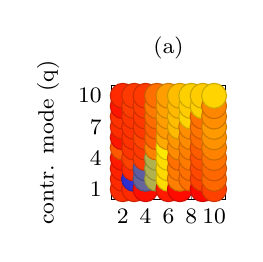
\begin{tikzpicture}
\begin{axis}
[
width=0.25\textwidth,
height=0.25\textwidth,
style={font=\footnotesize},
grid=major,
grid style={dotted},
align=center,
%xlabel={tensor order},
ylabel={contr. mode (q)},
title={{(a)}}, %  ompfor<slice>, asymmetric, row-major
scaled ticks=false,
zlabel={GFlops/core},
view={0}{90}, 
%view={-45}{45}, 
ytick={1,4,7,10},
xtick={2,4,6,8,10},
xmin=1, xmax=11,
ymin=0, ymax=11,
try min ticks=8,
zmin=0, zmax=50,
point meta min=0, point meta max=50,
colormap/hot, 
samples=50,
]
\addplot3[contour filled={number=100},scatter,shader=flat,samples=50]
coordinates{

(2.000,1.000,43.896) (2.000,2.000,44.316) (2.000,3.000,45.340) (2.000,4.000,46.159) (2.000,5.000,38.284) (2.000,6.000,46.700) (2.000,7.000,43.782) (2.000,8.000,43.238) (2.000,9.000,46.586) (2.000,10.000,44.445) 

(3.000,1.000,44.157) (3.000,2.000,3.488) (3.000,3.000,44.009) (3.000,4.000,41.443) (3.000,5.000,42.540) (3.000,6.000,43.421) (3.000,7.000,43.343) (3.000,8.000,42.638) (3.000,9.000,41.938) (3.000,10.000,42.175) 

(4.000,1.000,47.610) (4.000,2.000,6.548) (4.000,3.000,6.497) (4.000,4.000,41.914) (4.000,5.000,42.480) (4.000,6.000,40.513) (4.000,7.000,42.150) (4.000,8.000,42.362) (4.000,9.000,41.508) (4.000,10.000,42.485) 

(5.000,1.000,51.579) (5.000,2.000,11.839) (5.000,3.000,11.713) (5.000,4.000,11.721) (5.000,5.000,32.597) (5.000,6.000,36.602) (5.000,7.000,37.323) (5.000,8.000,35.667) (5.000,9.000,33.893) (5.000,10.000,35.328) 

(6.000,1.000,46.209) (6.000,2.000,21.375) (6.000,3.000,21.542) (6.000,4.000,21.382) (6.000,5.000,19.695) (6.000,6.000,27.921) (6.000,7.000,29.645) (6.000,8.000,29.213) (6.000,9.000,28.661) (6.000,10.000,29.405) 

(7.000,1.000,48.068) (7.000,2.000,33.377) (7.000,3.000,33.695) (7.000,4.000,35.053) (7.000,5.000,31.593) (7.000,6.000,30.136) (7.000,7.000,25.612) (7.000,8.000,25.054) (7.000,9.000,25.955) (7.000,10.000,25.248) 

(8.000,1.000,50.865) (8.000,2.000,35.412) (8.000,3.000,35.133) (8.000,4.000,33.799) (8.000,5.000,33.342) (8.000,6.000,31.890) (8.000,7.000,31.426) (8.000,8.000,22.371) (8.000,9.000,23.403) (8.000,10.000,22.843) 

(9.000,1.000,48.543) (9.000,2.000,41.355) (9.000,3.000,40.444) (9.000,4.000,39.428) (9.000,5.000,37.619) (9.000,6.000,35.552) (9.000,7.000,34.559) (9.000,8.000,35.278) (9.000,9.000,22.785) (9.000,10.000,23.178) 

(10.000,1.000,41.434) (10.000,2.000,36.469) (10.000,3.000,36.005) (10.000,4.000,34.970) (10.000,5.000,32.842) (10.000,6.000,30.760) (10.000,7.000,29.786) (10.000,8.000,31.179) (10.000,9.000,32.441) (10.000,10.000,22.265) 

};
\end{axis}
\end{tikzpicture}
\hfill
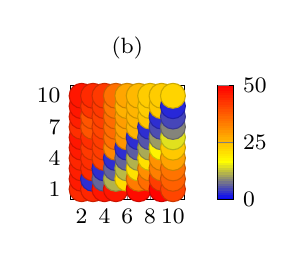
\begin{tikzpicture}
\begin{axis}
[
width=0.25\textwidth,
height=0.25\textwidth,
style={font=\footnotesize},
grid=major,
grid style={dotted},
align=center,
%xlabel={tensor order},
%ylabel={contr. mode (q)},
title={{(b)}}, %  ompfor<subtensor>, asymmetric, mkl
scaled ticks=false,
zlabel={GFlops},
view={0}{90}, 
ytick={1,4,7,10},
xtick={2,4,6,8,10},
xmin=1, xmax=11,
ymin=0, ymax=11,
try min ticks=8,
zmin=0, zmax=50,
point meta min=0, point meta max=50,
colormap/hot, 
samples=50,
colorbar sampled,
colorbar/width=0.2cm,
colorbar style={
	point meta min=0, point meta max=50,
	samples=50,
	font=\footnotesize,
	ytick={0,25,50},
	yticklabels={0,25,50},
	%title={\scriptsize Gflops},
	%ylabel={\scriptsize Gflops},
}
]
\addplot3[contour filled={number=100},scatter,shader=flat,samples=50]
coordinates{

(2.000,1.000,44.459) (2.000,2.000,46.351) (2.000,3.000,45.510) (2.000,4.000,44.636) (2.000,5.000,46.447) (2.000,6.000,46.641) (2.000,7.000,43.856) (2.000,8.000,45.859) (2.000,9.000,46.509) (2.000,10.000,46.686) 

(3.000,1.000,44.727) (3.000,2.000,3.490) (3.000,3.000,44.197) (3.000,4.000,43.861) (3.000,5.000,42.244) (3.000,6.000,43.848) (3.000,7.000,38.887) (3.000,8.000,38.650) (3.000,9.000,42.539) (3.000,10.000,44.223) 

(4.000,1.000,46.771) (4.000,2.000,6.537) (4.000,3.000,3.497) (4.000,4.000,41.114) (4.000,5.000,41.946) (4.000,6.000,41.889) (4.000,7.000,40.607) (4.000,8.000,41.455) (4.000,9.000,42.025) (4.000,10.000,41.998) 

(5.000,1.000,46.889) (5.000,2.000,11.964) (5.000,3.000,6.581) (5.000,4.000,3.465) (5.000,5.000,32.495) (5.000,6.000,35.170) (5.000,7.000,35.654) (5.000,8.000,35.862) (5.000,9.000,34.450) (5.000,10.000,35.248) 

(6.000,1.000,50.072) (6.000,2.000,21.383) (6.000,3.000,12.015) (6.000,4.000,6.500) (6.000,5.000,3.352) (6.000,6.000,30.066) (6.000,7.000,28.556) (6.000,8.000,29.463) (6.000,9.000,26.748) (6.000,10.000,28.155) 

(7.000,1.000,48.039) (7.000,2.000,33.621) (7.000,3.000,20.592) (7.000,4.000,11.558) (7.000,5.000,6.048) (7.000,6.000,3.278) (7.000,7.000,26.467) (7.000,8.000,26.394) (7.000,9.000,26.159) (7.000,10.000,25.519) 

(8.000,1.000,50.776) (8.000,2.000,35.546) (8.000,3.000,31.023) (8.000,4.000,20.828) (8.000,5.000,11.065) (8.000,6.000,5.837) (8.000,7.000,3.102) (8.000,8.000,24.096) (8.000,9.000,23.135) (8.000,10.000,23.270) 

(9.000,1.000,49.071) (9.000,2.000,41.747) (9.000,3.000,33.411) (9.000,4.000,30.777) (9.000,5.000,18.497) (9.000,6.000,10.262) (9.000,7.000,5.464) (9.000,8.000,3.133) (9.000,9.000,23.542) (9.000,10.000,23.357) 

(10.000,1.000,40.520) (10.000,2.000,37.272) (10.000,3.000,34.697) (10.000,4.000,28.652) (10.000,5.000,23.911) (10.000,6.000,14.900) (10.000,7.000,8.805) (10.000,8.000,4.918) (10.000,9.000,2.844) (10.000,10.000,22.469) 

};
\end{axis}
\end{tikzpicture}
\hfill
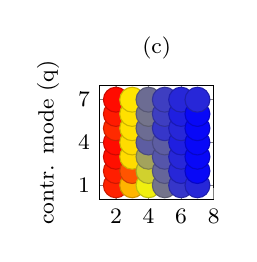
\begin{tikzpicture}
\begin{axis}
[
width=0.25\textwidth,
height=0.25\textwidth,
style={font=\footnotesize},
grid=major,
grid style={dotted},
align=center,
%xlabel={tensor order},
ylabel={contr. mode (q)},
title={{(c)}}, %  ompfor<slice>, symmetric, row-major
scaled ticks=false,
zlabel={GFlops},
view={0}{90}, 
ytick={1,4,7,10},
xtick={2,4,6,8},
xmin=1, xmax=8,
ymin=0, ymax=8,
try min ticks=8,
zmin=0, zmax=55,
point meta min=0, point meta max=55,
colormap/hot, 
samples=50,
]
\addplot3[contour filled={number=100},scatter,shader=flat,samples=50]
coordinates{

(2.000,1.000,49.884) (2.000,2.000,50.237) (2.000,3.000,52.259) (2.000,4.000,53.112) (2.000,5.000,48.642) (2.000,6.000,51.140) (2.000,7.000,53.264) 

(3.000,1.000,29.064) (3.000,2.000,42.832) (3.000,3.000,23.356) (3.000,4.000,23.347) (3.000,5.000,22.695) (3.000,6.000,22.978) (3.000,7.000,22.478) 

(4.000,1.000,17.083) (4.000,2.000,15.195) (4.000,3.000,12.081) (4.000,4.000,6.961) (4.000,5.000,8.128) (4.000,6.000,8.480) (4.000,7.000,8.210) 

(5.000,1.000,8.642) (5.000,2.000,7.699) (5.000,3.000,6.147) (5.000,4.000,6.635) (5.000,5.000,4.357) (5.000,6.000,4.476) (5.000,7.000,4.664) 

(6.000,1.000,4.335) (6.000,2.000,3.270) (6.000,3.000,2.956) (6.000,4.000,2.500) (6.000,5.000,2.807) (6.000,6.000,2.631) (6.000,7.000,2.772) 

(7.000,1.000,3.151) (7.000,2.000,0.567) (7.000,3.000,0.638) (7.000,4.000,0.650) (7.000,5.000,0.632) (7.000,6.000,0.649) (7.000,7.000,2.781) 


};
\end{axis}
\end{tikzpicture}
\hfill
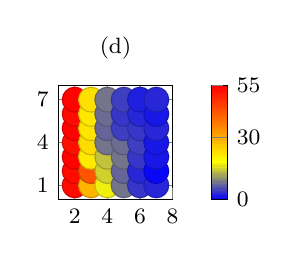
\begin{tikzpicture}
\begin{axis}
[
width=0.25\textwidth,
height=0.25\textwidth,
style={font=\footnotesize},
grid=major,
grid style={dotted},
align=center,
%xlabel={tensor order},
%ylabel={contr. mode (q)},
title={{(d)}}, %  ompfor<subtensor>, symmetric, row-major
scaled ticks=false,
zlabel={GFlops},
view={0}{90}, 
%view={-45}{45}, 
ytick={1,4,7,10},
xtick={2,4,6,8},
xmin=1, xmax=8,
ymin=0, ymax=8,
try min ticks=8,
zmin=0, zmax=55,
point meta min=0, point meta max=55,
colormap/hot, 
samples=50,
colorbar sampled,
colorbar/width=0.2cm,
colorbar style={
	point meta min=0, point meta max=55,
	samples=50,
	font=\footnotesize,
	ytick={0,30,55},
	yticklabels={0,30,55},
	%title={\scriptsize Gflops},
	%ylabel={\scriptsize Gflops},
}
]
\addplot3[contour filled={number=100},scatter,shader=flat,samples=50]
coordinates{

(2.000,1.000,52.847) (2.000,2.000,53.105) (2.000,3.000,54.140) (2.000,4.000,52.620) (2.000,5.000,53.976) (2.000,6.000,53.003) (2.000,7.000,53.953) 

(3.000,1.000,28.660) (3.000,2.000,42.680) (3.000,3.000,21.118) (3.000,4.000,23.419) (3.000,5.000,22.416) (3.000,6.000,21.925) (3.000,7.000,22.886) 

(4.000,1.000,17.375) (4.000,2.000,15.257) (4.000,3.000,13.767) (4.000,4.000,8.621) (4.000,5.000,7.667) (4.000,6.000,7.963) (4.000,7.000,8.423) 

(5.000,1.000,8.648) (5.000,2.000,7.667) (5.000,3.000,8.572) (5.000,4.000,7.742) (5.000,5.000,4.437) (5.000,6.000,4.127) (5.000,7.000,4.642) 

(6.000,1.000,4.295) (6.000,2.000,3.270) (6.000,3.000,4.016) (6.000,4.000,4.522) (6.000,5.000,3.888) (6.000,6.000,2.759) (6.000,7.000,2.713) 

(7.000,1.000,3.143) (7.000,2.000,0.571) (7.000,3.000,1.910) (7.000,4.000,1.785) (7.000,5.000,2.751) (7.000,6.000,1.807) (7.000,7.000,3.058) 


};
\end{axis}
\end{tikzpicture}  %parloop
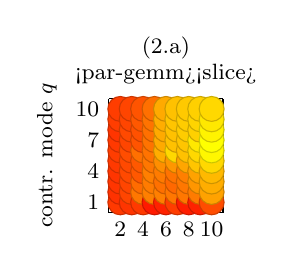
\begin{tikzpicture}
\begin{axis}
[
width=0.25\textwidth,
height=0.25\textwidth,
style={font=\footnotesize},
grid=major,
grid style={dotted},
align=center,
%xlabel={tensor order},
ylabel={contr. mode $q$},
title={(2.a)\\\tss{<par-gemm><slice>}}, %  pargemm<slice>, asymmetric, row-major, mkl
title style={yshift=-1ex},
scaled ticks=false,
zlabel={GFlops/core},
view={0}{90}, 
%view={-45}{45}, 
ytick={1,4,7,10},
xtick={2,4,6,8,10},
xmin=1, xmax=11,
ymin=0, ymax=11,
try min ticks=8,
zmin=0, zmax=55,
point meta min=0, point meta max=55,
colormap/hot, 
samples=55,
]
\addplot3[contour filled={number=100},scatter,shader=flat,samples=55]
coordinates{
(2.000,1.000,46.317) (2.000,2.000,47.467) (2.000,3.000,46.785) (2.000,4.000,46.908) (2.000,5.000,46.657) (2.000,6.000,45.822) (2.000,7.000,46.501) (2.000,8.000,47.166) (2.000,9.000,45.817) (2.000,10.000,45.838) 

(3.000,1.000,46.799) (3.000,2.000,44.592) (3.000,3.000,44.972) (3.000,4.000,44.132) (3.000,5.000,44.473) (3.000,6.000,43.555) (3.000,7.000,45.048) (3.000,8.000,44.306) (3.000,9.000,44.715) (3.000,10.000,44.711) 

(4.000,1.000,46.289) (4.000,2.000,37.746) (4.000,3.000,39.173) (4.000,4.000,42.161) (4.000,5.000,42.303) (4.000,6.000,39.003) (4.000,7.000,42.644) (4.000,8.000,43.034) (4.000,9.000,41.854) (4.000,10.000,42.895) 

(5.000,1.000,50.964) (5.000,2.000,36.480) (5.000,3.000,37.083) (5.000,4.000,36.474) (5.000,5.000,37.539) (5.000,6.000,38.234) (5.000,7.000,38.204) (5.000,8.000,38.503) (5.000,9.000,37.973) (5.000,10.000,38.626) 

(6.000,1.000,49.775) (6.000,2.000,36.594) (6.000,3.000,38.549) (6.000,4.000,37.212) (6.000,5.000,34.515) (6.000,6.000,30.085) (6.000,7.000,30.745) (6.000,8.000,30.647) (6.000,9.000,30.171) (6.000,10.000,30.565) 

(7.000,1.000,46.098) (7.000,2.000,37.478) (7.000,3.000,39.858) (7.000,4.000,38.195) (7.000,5.000,33.103) (7.000,6.000,23.667) (7.000,7.000,26.990) (7.000,8.000,27.232) (7.000,9.000,26.693) (7.000,10.000,27.254) 

(8.000,1.000,50.490) (8.000,2.000,37.502) (8.000,3.000,37.745) (8.000,4.000,36.398) (8.000,5.000,31.315) (8.000,6.000,27.314) (8.000,7.000,26.440) (8.000,8.000,25.665) (8.000,9.000,25.704) (8.000,10.000,25.867) 

(9.000,1.000,49.745) (9.000,2.000,37.042) (9.000,3.000,33.158) (9.000,4.000,31.522) (9.000,5.000,26.570) (9.000,6.000,23.876) (9.000,7.000,21.588) (9.000,8.000,24.772) (9.000,9.000,24.220) (9.000,10.000,24.867) 

(10.000,1.000,43.680) (10.000,2.000,31.533) (10.000,3.000,30.229) (10.000,4.000,28.157) (10.000,5.000,23.743) (10.000,6.000,19.455) (10.000,7.000,18.637) (10.000,8.000,19.922) (10.000,9.000,21.995) (10.000,10.000,23.892) 


};
\end{axis}
\end{tikzpicture}
\hfill
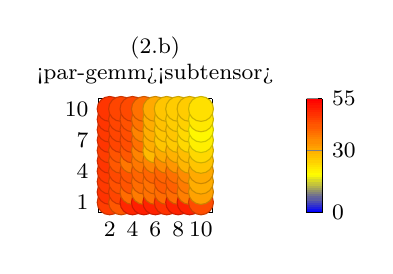
\begin{tikzpicture}
\begin{axis}
[
width=0.25\textwidth,
height=0.25\textwidth,
style={font=\footnotesize},
grid=major,
grid style={dotted},
align=center,
%xlabel={tensor order},
%ylabel={contr. mode (q)},
title={(2.b)\\\tss{<par-gemm><subtensor>}}, %  pargemm<subtensor>, asymmetric, mkl, row.major
title style={yshift=-1ex},
scaled ticks=false,
zlabel={GFlops},
view={0}{90}, 
ytick={1,4,7,10},
xtick={2,4,6,8,10},
xmin=1, xmax=11,
ymin=0, ymax=11,
try min ticks=8,
zmin=0, zmax=55,
point meta min=0, point meta max=55,
colormap/hot, 
samples=55,
colorbar sampled,
colorbar/width=0.2cm,
colorbar style={
point meta min=0, point meta max=55,
samples=55,
font=\footnotesize,
ytick={0,30,55},
yticklabels={0,30,55},
%title={\scriptsize Gflops},
%ylabel={\scriptsize Gflops},
}
]
\addplot3[contour filled={number=100},scatter,shader=flat,samples=55]
coordinates{

(2.000,1.000,46.024) (2.000,2.000,47.499) (2.000,3.000,46.518) (2.000,4.000,46.647) (2.000,5.000,46.939) (2.000,6.000,45.807) (2.000,7.000,46.788) (2.000,8.000,46.201) (2.000,9.000,46.824) (2.000,10.000,46.817) 

(3.000,1.000,41.968) (3.000,2.000,44.618) (3.000,3.000,43.239) (3.000,4.000,44.176) (3.000,5.000,42.190) (3.000,6.000,42.685) (3.000,7.000,44.634) (3.000,8.000,44.551) (3.000,9.000,45.078) (3.000,10.000,44.656) 

(4.000,1.000,49.206) (4.000,2.000,39.114) (4.000,3.000,42.621) (4.000,4.000,42.869) (4.000,5.000,37.872) (4.000,6.000,41.893) (4.000,7.000,43.549) (4.000,8.000,43.776) (4.000,9.000,43.074) (4.000,10.000,44.055) 

(5.000,1.000,50.432) (5.000,2.000,37.339) (5.000,3.000,39.583) (5.000,4.000,40.371) (5.000,5.000,37.481) (5.000,6.000,36.183) (5.000,7.000,38.874) (5.000,8.000,36.295) (5.000,9.000,38.334) (5.000,10.000,38.828) 

(6.000,1.000,49.563) (6.000,2.000,39.033) (6.000,3.000,38.729) (6.000,4.000,40.488) (6.000,5.000,35.766) (6.000,6.000,28.574) (6.000,7.000,30.137) (6.000,8.000,29.909) (6.000,9.000,30.071) (6.000,10.000,30.335) 

(7.000,1.000,47.837) (7.000,2.000,39.558) (7.000,3.000,41.754) (7.000,4.000,40.236) (7.000,5.000,34.661) (7.000,6.000,30.281) (7.000,7.000,26.674) (7.000,8.000,26.594) (7.000,9.000,27.319) (7.000,10.000,26.694) 

(8.000,1.000,49.852) (8.000,2.000,39.408) (8.000,3.000,41.192) (8.000,4.000,38.730) (8.000,5.000,33.342) (8.000,6.000,29.655) (8.000,7.000,26.196) (8.000,8.000,26.772) (8.000,9.000,25.778) (8.000,10.000,25.490) 

(9.000,1.000,49.752) (9.000,2.000,36.678) (9.000,3.000,36.985) (9.000,4.000,34.654) (9.000,5.000,29.039) (9.000,6.000,27.701) (9.000,7.000,24.123) (9.000,8.000,24.053) (9.000,9.000,25.007) (9.000,10.000,25.359) 

(10.000,1.000,43.556) (10.000,2.000,31.723) (10.000,3.000,30.114) (10.000,4.000,30.474) (10.000,5.000,26.695) (10.000,6.000,24.184) (10.000,7.000,20.683) (10.000,8.000,19.787) (10.000,9.000,21.875) (10.000,10.000,22.884) 


};
\end{axis}
\end{tikzpicture}
\hfill
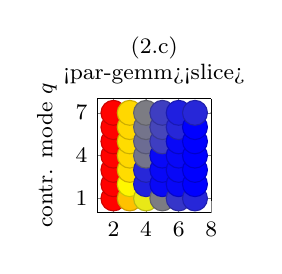
\begin{tikzpicture}
\begin{axis}
[
width=0.25\textwidth,
height=0.25\textwidth,
style={font=\footnotesize},
grid=major,
grid style={dotted},
align=center,
%xlabel={tensor order},
ylabel={contr. mode $q$},
title={(2.c)\\\tss{<par-gemm><slice>}}, %  pargemm<slice>, symmetric, row-major
title style={yshift=-1ex},
scaled ticks=false,
zlabel={GFlops},
view={0}{90}, 
ytick={1,4,7,10},
xtick={2,4,6,8},
xmin=1, xmax=8,
ymin=0, ymax=8,
try min ticks=8,
zmin=0, zmax=55,
point meta min=0, point meta max=55,
colormap/hot, 
samples=55
]
\addplot3[contour filled={number=100},scatter,shader=flat,samples=55]
coordinates{

(2.000,1.000,54.069) (2.000,2.000,54.524) (2.000,3.000,54.079) (2.000,4.000,54.441) (2.000,5.000,54.500) (2.000,6.000,54.168) (2.000,7.000,54.447) 

(3.000,1.000,27.294) (3.000,2.000,19.589) (3.000,3.000,23.485) (3.000,4.000,23.978) (3.000,5.000,23.522) (3.000,6.000,24.035) (3.000,7.000,23.660) 

(4.000,1.000,16.871) (4.000,2.000,2.541) (4.000,3.000,2.842) (4.000,4.000,8.714) (4.000,5.000,8.244) (4.000,6.000,8.648) (4.000,7.000,8.818) 

(5.000,1.000,8.873) (5.000,2.000,0.844) (5.000,3.000,0.856) (5.000,4.000,0.854) (5.000,5.000,4.875) (5.000,6.000,5.034) (5.000,7.000,4.445) 

(6.000,1.000,4.355) (6.000,2.000,0.570) (6.000,3.000,0.575) (6.000,4.000,0.623) (6.000,5.000,0.593) (6.000,6.000,2.899) (6.000,7.000,2.728) 

(7.000,1.000,3.255) (7.000,2.000,0.244) (7.000,3.000,0.159) (7.000,4.000,0.251) (7.000,5.000,0.264) (7.000,6.000,0.258) (7.000,7.000,3.065) 


};
\end{axis}
\end{tikzpicture}
\hfill
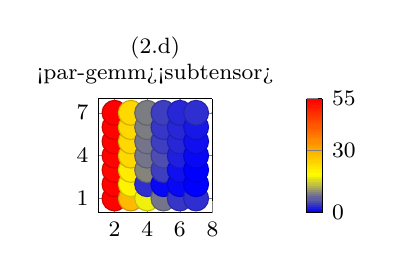
\begin{tikzpicture}
\begin{axis}
[
width=0.25\textwidth,
height=0.25\textwidth,
style={font=\footnotesize},
grid=major,
grid style={dotted},
align=center,
%xlabel={tensor order},
%ylabel={contr. mode (q)},
title={(2.d)\\\tss{<par-gemm><subtensor>}}, %  pargemm<subtensor>, symmetric, row-major
title style={yshift=-1ex},
scaled ticks=false,
zlabel={GFlops},
view={0}{90}, 
%view={-45}{45}, 
ytick={1,4,7,10},
xtick={2,4,6,8},
xmin=1, xmax=8,
ymin=0, ymax=8,
try min ticks=8,
zmin=0, zmax=55,
point meta min=0, point meta max=55,
colormap/hot, 
colorbar sampled,
colorbar/width=0.2cm,
colorbar style={
point meta min=0, point meta max=55,
font=\footnotesize,
ytick={0,30,55},
yticklabels={0,30,55},
samples=55
%title={\scriptsize Gflops},
%ylabel={\scriptsize Gflops},
}
]
\addplot3[contour filled={number=100},scatter,shader=flat,samples=55]
coordinates{

(2.000,1.000,54.044) (2.000,2.000,54.235) (2.000,3.000,53.780) (2.000,4.000,54.392) (2.000,5.000,54.142) (2.000,6.000,53.918) (2.000,7.000,54.583) 

(3.000,1.000,28.060) (3.000,2.000,19.851) (3.000,3.000,21.251) (3.000,4.000,23.673) (3.000,5.000,23.690) (3.000,6.000,23.943) (3.000,7.000,23.887) 

(4.000,1.000,17.114) (4.000,2.000,3.369) (4.000,3.000,9.529) (4.000,4.000,8.731) (4.000,5.000,8.373) (4.000,6.000,8.989) (4.000,7.000,8.866) 

(5.000,1.000,8.728) (5.000,2.000,0.898) (5.000,3.000,4.591) (5.000,4.000,5.693) (5.000,5.000,4.813) (5.000,6.000,4.240) (5.000,7.000,4.917) 

(6.000,1.000,4.370) (6.000,2.000,0.573) (6.000,3.000,1.397) (6.000,4.000,2.626) (6.000,5.000,2.874) (6.000,6.000,2.815) (6.000,7.000,2.828) 

(7.000,1.000,3.777) (7.000,2.000,0.243) (7.000,3.000,0.303) (7.000,4.000,0.649) (7.000,5.000,1.255) (7.000,6.000,1.973) (7.000,7.000,3.407) 



};
\end{axis}
\end{tikzpicture}  
%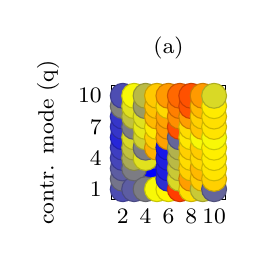
\begin{tikzpicture}
\begin{axis}
[
width=0.25\textwidth,
height=0.25\textwidth,
style={font=\footnotesize},
grid=major,
grid style={dotted},
align=center,
%xlabel={tensor order},
ylabel={contr. mode (q)},
title={{(a)}}, %  ompfor<slice>, asymmetric, row-major
scaled ticks=false,
zlabel={GFlops/core},
view={0}{90}, 
%view={-45}{45}, 
ytick={1,4,7,10},
xtick={2,4,6,8,10},
xmin=1, xmax=11,
ymin=0, ymax=11,
try min ticks=8,
zmin=10, zmax=50,
point meta min=10, point meta max=50,
colormap/hot, 
samples=50,
]
\addplot3[contour filled={number=100},scatter,shader=flat,samples=50]
coordinates{

(2.000,1.000,14.177) (2.000,2.000,16.358) (2.000,3.000,14.869) (2.000,4.000,13.784) (2.000,5.000,13.218) (2.000,6.000,12.389) (2.000,7.000,12.811) (2.000,8.000,13.152) (2.000,9.000,17.167) (2.000,10.000,14.058) 

(3.000,1.000,14.928) (3.000,2.000,1.784) (3.000,3.000,16.681) (3.000,4.000,18.809) (3.000,5.000,20.087) (3.000,6.000,21.317) (3.000,7.000,16.786) (3.000,8.000,20.171) (3.000,9.000,21.800) (3.000,10.000,22.919) 

(4.000,1.000,16.621) (4.000,2.000,3.476) (4.000,3.000,3.324) (4.000,4.000,21.715) (4.000,5.000,16.734) (4.000,6.000,20.909) (4.000,7.000,22.252) (4.000,8.000,21.890) (4.000,9.000,18.106) (4.000,10.000,19.650) 

(5.000,1.000,23.063) (5.000,2.000,6.656) (5.000,3.000,6.354) (5.000,4.000,6.245) (5.000,5.000,31.276) (5.000,6.000,28.747) (5.000,7.000,25.870) (5.000,8.000,30.670) (5.000,9.000,29.994) (5.000,10.000,28.934) 

(6.000,1.000,24.099) (6.000,2.000,12.542) (6.000,3.000,11.879) (6.000,4.000,11.622) (6.000,5.000,11.371) (6.000,6.000,33.174) (6.000,7.000,33.505) (6.000,8.000,33.144) (6.000,9.000,27.321) (6.000,10.000,33.741) 

(7.000,1.000,43.545) (7.000,2.000,21.351) (7.000,3.000,20.534) (7.000,4.000,19.951) (7.000,5.000,19.439) (7.000,6.000,15.298) (7.000,7.000,41.259) (7.000,8.000,35.160) (7.000,9.000,36.637) (7.000,10.000,38.996) 

(8.000,1.000,26.764) (8.000,2.000,33.491) (8.000,3.000,28.294) (8.000,4.000,26.895) (8.000,5.000,28.272) (8.000,6.000,25.903) (8.000,7.000,26.818) (8.000,8.000,33.547) (8.000,9.000,40.813) (8.000,10.000,41.255) 

(9.000,1.000,20.798) (9.000,2.000,28.583) (9.000,3.000,30.483) (9.000,4.000,27.264) (9.000,5.000,28.433) (9.000,6.000,22.847) (9.000,7.000,29.367) (9.000,8.000,28.364) (9.000,9.000,30.574) (9.000,10.000,33.672) 

(10.000,1.000,15.559) (10.000,2.000,28.090) (10.000,3.000,26.263) (10.000,4.000,25.477) (10.000,5.000,24.815) (10.000,6.000,22.805) (10.000,7.000,26.381) (10.000,8.000,26.505) (10.000,9.000,25.500) (10.000,10.000,21.425) 

};
\end{axis}
\end{tikzpicture}
\hfill
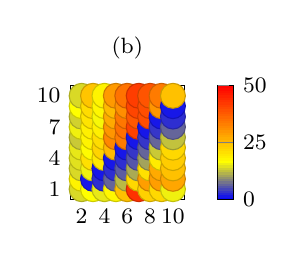
\begin{tikzpicture}
\begin{axis}
[
width=0.25\textwidth,
height=0.25\textwidth,
style={font=\footnotesize},
grid=major,
grid style={dotted},
align=center,
%xlabel={tensor order},
%ylabel={contr. mode (q)},
title={{(b)}}, %  ompfor<subtensor>, asymmetric, row-major
scaled ticks=false,
zlabel={GFlops},
view={0}{90}, 
ytick={1,4,7,10},
xtick={2,4,6,8,10},
xmin=1, xmax=11,
ymin=0, ymax=11,
try min ticks=8,
zmin=0, zmax=50,
point meta min=0, point meta max=50,
colormap/hot, 
samples=50,
colorbar sampled,
colorbar/width=0.2cm,
colorbar style={
point meta min=0, point meta max=50,
samples=50,
font=\footnotesize,
ytick={0,25,50},
yticklabels={0,25,50},
%title={\scriptsize Gflops},
%ylabel={\scriptsize Gflops},
}
]
\addplot3[contour filled={number=100},scatter,shader=flat,samples=50]
coordinates{

(2.000,1.000,14.150) (2.000,2.000,18.168) (2.000,3.000,14.380) (2.000,4.000,14.818) (2.000,5.000,15.416) (2.000,6.000,13.081) (2.000,7.000,15.551) (2.000,8.000,13.981) (2.000,9.000,16.961) (2.000,10.000,14.297) 

(3.000,1.000,16.658) (3.000,2.000,1.780) (3.000,3.000,15.940) (3.000,4.000,20.908) (3.000,5.000,17.001) (3.000,6.000,18.151) (3.000,7.000,18.853) (3.000,8.000,20.356) (3.000,9.000,21.150) (3.000,10.000,24.034) 

(4.000,1.000,15.470) (4.000,2.000,3.473) (4.000,3.000,1.763) (4.000,4.000,19.978) (4.000,5.000,22.019) (4.000,6.000,21.370) (4.000,7.000,18.694) (4.000,8.000,16.418) (4.000,9.000,17.892) (4.000,10.000,18.183) 

(5.000,1.000,17.885) (5.000,2.000,6.625) (5.000,3.000,3.373) (5.000,4.000,1.701) (5.000,5.000,25.808) (5.000,6.000,32.283) (5.000,7.000,30.427) (5.000,8.000,27.599) (5.000,9.000,25.759) (5.000,10.000,29.893) 

(6.000,1.000,24.716) (6.000,2.000,12.440) (6.000,3.000,6.321) (6.000,4.000,3.193) (6.000,5.000,1.782) (6.000,6.000,33.517) (6.000,7.000,35.466) (6.000,8.000,34.242) (6.000,9.000,31.231) (6.000,10.000,34.605) 

(7.000,1.000,43.408) (7.000,2.000,21.521) (7.000,3.000,11.123) (7.000,4.000,5.561) (7.000,5.000,3.508) (7.000,6.000,1.784) (7.000,7.000,41.398) (7.000,8.000,38.079) (7.000,9.000,40.652) (7.000,10.000,41.770) 

(8.000,1.000,22.875) (8.000,2.000,29.491) (8.000,3.000,20.653) (8.000,4.000,10.787) (8.000,5.000,6.814) (8.000,6.000,3.511) (8.000,7.000,1.788) (8.000,8.000,39.967) (8.000,9.000,39.718) (8.000,10.000,38.518) 

(9.000,1.000,21.665) (9.000,2.000,29.387) (9.000,3.000,27.538) (9.000,4.000,19.369) (9.000,5.000,13.041) (9.000,6.000,6.810) (9.000,7.000,3.504) (9.000,8.000,1.769) (9.000,9.000,30.494) (9.000,10.000,33.784) 

(10.000,1.000,15.677) (10.000,2.000,28.056) (10.000,3.000,24.845) (10.000,4.000,23.423) (10.000,5.000,21.554) (10.000,6.000,12.533) (10.000,7.000,6.784) (10.000,8.000,3.476) (10.000,9.000,1.758) (10.000,10.000,24.585) 


};
\end{axis}
\end{tikzpicture}
\hfill
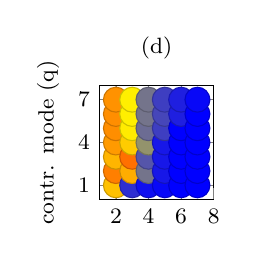
\begin{tikzpicture}
\begin{axis}
[
width=0.25\textwidth,
height=0.25\textwidth,
style={font=\footnotesize},
grid=major,
grid style={dotted},
align=center,
%xlabel={tensor order},
ylabel={contr. mode (q)},
title={{(d)}}, %  ompfor<slice>, symmetric, row-major
scaled ticks=false,
zlabel={GFlops},
view={0}{90}, 
ytick={1,4,7,10},
xtick={2,4,6,8},
xmin=1, xmax=8,
ymin=0, ymax=8,
try min ticks=8,
zmin=0, zmax=55,
point meta min=0, point meta max=55,
colormap/hot, 
samples=50,
]
\addplot3[contour filled={number=100},scatter,shader=flat,samples=50]
coordinates{

(2.000,1.000,27.090) (2.000,2.000,36.633) (2.000,3.000,28.737) (2.000,4.000,32.791) (2.000,5.000,34.606) (2.000,6.000,34.332) (2.000,7.000,33.607) 

(3.000,1.000,3.535) (3.000,2.000,30.198) (3.000,3.000,38.963) (3.000,4.000,25.423) (3.000,5.000,21.062) (3.000,6.000,20.381) (3.000,7.000,20.382) 

(4.000,1.000,1.243) (4.000,2.000,8.485) (4.000,3.000,6.219) (4.000,4.000,10.477) (4.000,5.000,8.056) (4.000,6.000,8.354) (4.000,7.000,8.337) 

(5.000,1.000,0.702) (5.000,2.000,1.700) (5.000,3.000,1.650) (5.000,4.000,1.662) (5.000,5.000,4.782) (5.000,6.000,5.217) (5.000,7.000,4.731) 

(6.000,1.000,0.391) (6.000,2.000,0.218) (6.000,3.000,0.219) (6.000,4.000,0.219) (6.000,5.000,0.220) (6.000,6.000,2.476) (6.000,7.000,2.653) 

(7.000,1.000,0.307) (7.000,2.000,0.026) (7.000,3.000,0.027) (7.000,4.000,0.027) (7.000,5.000,0.027) (7.000,6.000,0.027) (7.000,7.000,0.839) 


};
\end{axis}
\end{tikzpicture}
\hfill
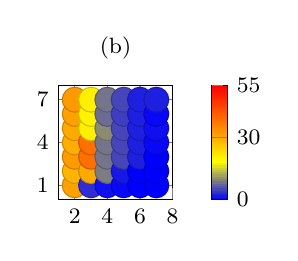
\begin{tikzpicture}
\begin{axis}
[
width=0.25\textwidth,
height=0.25\textwidth,
style={font=\footnotesize},
grid=major,
grid style={dotted},
align=center,
%xlabel={tensor order},
%ylabel={contr. mode (q)},
title={{(b)}}, %  ompfor<subtensor>, symmetric, row-major
scaled ticks=false,
zlabel={GFlops},
view={0}{90}, 
%view={-45}{45}, 
ytick={1,4,7,10},
xtick={2,4,6,8},
xmin=1, xmax=8,
ymin=0, ymax=8,
try min ticks=8,
zmin=0, zmax=55,
point meta min=0, point meta max=55,
colormap/hot, 
samples=50,
colorbar sampled,
colorbar/width=0.2cm,
colorbar style={
point meta min=0, point meta max=55,
samples=50,
font=\footnotesize,
ytick={0,30,55},
yticklabels={0,30,55},
%title={\scriptsize Gflops},
%ylabel={\scriptsize Gflops},
}
]
\addplot3[contour filled={number=100},scatter,shader=flat,samples=50]
coordinates{

(2.000,1.000,31.720) (2.000,2.000,28.835) (2.000,3.000,32.560) (2.000,4.000,29.729) (2.000,5.000,30.367) (2.000,6.000,31.442) (2.000,7.000,32.686) 

(3.000,1.000,3.525) (3.000,2.000,30.655) (3.000,3.000,38.818) (3.000,4.000,38.927) (3.000,5.000,20.463) (3.000,6.000,20.182) (3.000,7.000,20.852) 

(4.000,1.000,1.205) (4.000,2.000,9.073) (4.000,3.000,8.324) (4.000,4.000,8.252) (4.000,5.000,9.954) (4.000,6.000,7.973) (4.000,7.000,8.301) 

(5.000,1.000,0.658) (5.000,2.000,1.760) (5.000,3.000,5.100) (5.000,4.000,5.138) (5.000,5.000,5.269) (5.000,6.000,4.879) (5.000,7.000,4.964) 

(6.000,1.000,0.331) (6.000,2.000,0.219) (6.000,3.000,2.300) (6.000,4.000,2.632) (6.000,5.000,2.349) (6.000,6.000,2.437) (6.000,7.000,2.383) 

(7.000,1.000,0.310) (7.000,2.000,0.026) (7.000,3.000,0.360) (7.000,4.000,0.846) (7.000,5.000,1.135) (7.000,6.000,0.930) (7.000,7.000,2.590) 


};
\end{axis}
\end{tikzpicture}
\caption{%
\footnotesize %
Performance contour plots in double-precision Gflops per core of the proposed TTM algorithms \tf{<par-loop>} and \tf{<par-gemm>} with varying tensor orders $p$ and contraction modes $q$. 
The top row of maps (1.x) depict measurements of the \tf{<par-loop>} versions while bottom row of maps with number (2.x) contain measurements of the \tf{<par-gemm>} versions.
Tensors are asymmetrically shaped on the left four maps (a,b) and symmetrically shaped on the right four maps (c,d).
Tensor $\mubA$ and $\mubC$ have the first-order while matrix $\mbB$ has the row-major ordering.
All functions have been measured on the Intel Xeon Gold 5318Y processor.
\label{fig:performance.tlib.contour}
}
\end{figure*}


\begin{figure*}[t]
\centering
%\tikzset{every mark/.append style={scale=1.5}}
\begin{tikzpicture}
\begin{axis}[
height=0.2\textheight,
width=0.25\textwidth,
style={font=\footnotesize},
grid=major,
grid style={dotted},
align=center,
%xlabel={Tflops},
ylabel={Cumulative Probability},
ylabel near ticks,
title={(a)}, % intel(mkl) - (ttm<rm>) asymmetric
xtick={0,15,30,45},
xticklabels={0,15,30,45},
xmax=47,
ytick={0,0.25,0.5,0.75,1},
yticklabels={0,0.25,0.5,0.75,1},
mark repeat={16},
cycle list name=compare case 8 for mkl
]

\addplot
coordinates{(5.766,0.000) (5.766,0.004) (6.030,0.009) (6.453,0.013) (6.651,0.018) (6.727,0.022) (6.839,0.027) (6.936,0.031) (6.981,0.036) (9.199,0.040) (9.441,0.045) (9.971,0.049) (11.274,0.054) (11.278,0.058) (11.307,0.062) (11.328,0.067) (11.358,0.071) (11.365,0.076) (11.839,0.080) (11.949,0.085) (12.239,0.089) (12.252,0.094) (12.280,0.098) (12.347,0.103) (12.588,0.107) (12.712,0.112) (12.745,0.116) (12.844,0.121) (12.856,0.125) (12.895,0.129) (13.825,0.134) (14.730,0.138) (18.446,0.143) (20.022,0.147) (20.256,0.152) (20.607,0.156) (20.884,0.161) (21.001,0.165) (21.017,0.170) (21.047,0.174) (21.068,0.179) (21.126,0.183) (21.248,0.188) (21.297,0.192) (21.389,0.196) (21.406,0.201) (21.428,0.205) (21.454,0.210) (21.495,0.214) (21.586,0.219) (21.730,0.223) (21.755,0.228) (21.769,0.232) (21.917,0.237) (22.008,0.241) (22.153,0.246) (22.515,0.250) (22.729,0.254) (22.831,0.259) (22.948,0.263) (22.961,0.268) (23.647,0.272) (23.801,0.277) (24.716,0.281) (25.609,0.286) (26.002,0.290) (26.941,0.295) (27.022,0.299) (27.268,0.304) (27.294,0.308) (28.215,0.312) (28.495,0.317) (28.672,0.321) (28.776,0.326) (28.825,0.330) (29.563,0.335) (29.601,0.339) (29.603,0.344) (30.221,0.348) (31.020,0.353) (31.034,0.357) (31.193,0.362) (31.269,0.366) (31.318,0.371) (31.395,0.375) (31.742,0.379) (31.844,0.384) (31.857,0.388) (31.973,0.393) (32.142,0.397) (32.384,0.402) (32.387,0.406) (32.448,0.411) (32.593,0.415) (32.770,0.420) (32.778,0.424) (32.811,0.429) (32.862,0.433) (32.880,0.437) (33.267,0.442) (33.314,0.446) (33.360,0.451) (33.365,0.455) (33.749,0.460) (33.763,0.464) (33.766,0.469) (33.807,0.473) (33.845,0.478) (33.919,0.482) (34.028,0.487) (34.040,0.491) (34.060,0.496) (34.118,0.500) (34.132,0.504) (34.172,0.509) (34.183,0.513) (34.215,0.518) (34.250,0.522) (34.290,0.527) (34.344,0.531) (34.432,0.536) (34.514,0.540) (34.547,0.545) (34.598,0.549) (34.614,0.554) (34.636,0.558) (34.692,0.562) (34.870,0.567) (34.924,0.571) (34.966,0.576) (34.984,0.580) (34.999,0.585) (35.155,0.589) (35.246,0.594) (35.284,0.598) (35.320,0.603) (35.329,0.607) (35.391,0.612) (35.456,0.616) (35.571,0.621) (35.604,0.625) (35.631,0.629) (35.716,0.634) (35.770,0.638) (35.804,0.643) (35.812,0.647) (35.830,0.652) (35.889,0.656) (35.941,0.661) (35.947,0.665) (36.080,0.670) (36.154,0.674) (36.164,0.679) (36.302,0.683) (36.418,0.688) (36.430,0.692) (36.468,0.696) (36.500,0.701) (36.640,0.705) (36.691,0.710) (36.728,0.714) (36.803,0.719) (36.824,0.723) (36.846,0.728) (36.895,0.732) (36.920,0.737) (36.993,0.741) (37.164,0.746) (37.385,0.750) (37.413,0.754) (37.476,0.759) (37.485,0.763) (38.161,0.768) (38.271,0.772) (38.279,0.777) (38.394,0.781) (38.663,0.786) (38.688,0.790) (38.817,0.795) (38.886,0.799) (39.055,0.804) (39.148,0.808) (39.166,0.812) (39.449,0.817) (39.964,0.821) (40.031,0.826) (40.105,0.830) (40.150,0.835) (40.200,0.839) (40.263,0.844) (40.442,0.848) (40.577,0.853) (40.638,0.857) (40.675,0.862) (40.749,0.866) (40.888,0.871) (40.915,0.875) (41.161,0.879) (41.204,0.884) (41.360,0.888) (41.370,0.893) (41.482,0.897) (41.750,0.902) (41.989,0.906) (42.097,0.911) (42.111,0.915) (42.441,0.920) (42.544,0.924) (42.574,0.929) (42.767,0.933) (42.944,0.938) (43.450,0.942) (43.574,0.946) (43.909,0.951) (44.220,0.955) (44.360,0.960) (44.687,0.964) (44.725,0.969) (44.791,0.973) (45.280,0.978) (45.396,0.982) (45.464,0.987) (46.146,0.991) (46.254,0.996) (46.354,1.000) };

\addplot
coordinates{(2.500,0.000) (2.500,0.004) (3.892,0.009) (3.907,0.013) (3.913,0.018) (4.807,0.022) (4.910,0.027) (4.928,0.031) (5.090,0.036) (5.268,0.040) (5.290,0.045) (5.325,0.049) (5.371,0.054) (5.627,0.058) (5.629,0.062) (5.653,0.067) (5.660,0.071) (5.741,0.076) (5.756,0.080) (5.771,0.085) (5.872,0.089) (5.872,0.094) (5.874,0.098) (5.947,0.103) (5.960,0.107) (5.963,0.112) (6.002,0.116) (6.004,0.121) (6.019,0.125) (6.042,0.129) (6.044,0.134) (6.077,0.138) (6.119,0.143) (6.131,0.147) (6.188,0.152) (6.211,0.156) (6.262,0.161) (6.318,0.165) (6.333,0.170) (6.337,0.174) (6.352,0.179) (6.359,0.183) (6.452,0.188) (6.491,0.192) (6.523,0.196) (6.539,0.201) (6.653,0.205) (6.688,0.210) (6.793,0.214) (6.859,0.219) (6.863,0.223) (6.864,0.228) (6.921,0.232) (6.951,0.237) (6.954,0.241) (6.981,0.246) (7.006,0.250) (7.013,0.254) (7.018,0.259) (7.046,0.263) (7.546,0.268) (8.353,0.272) (8.956,0.277) (9.275,0.281) (9.480,0.286) (9.578,0.290) (9.882,0.295) (9.961,0.299) (9.980,0.304) (10.113,0.308) (10.277,0.312) (10.326,0.317) (10.341,0.321) (10.447,0.326) (10.469,0.330) (10.588,0.335) (10.730,0.339) (10.860,0.344) (10.901,0.348) (10.967,0.353) (11.004,0.357) (11.136,0.362) (11.139,0.366) (11.298,0.371) (11.305,0.375) (11.329,0.379) (11.439,0.384) (11.455,0.388) (11.573,0.393) (11.624,0.397) (11.838,0.402) (11.906,0.406) (11.984,0.411) (11.988,0.415) (11.995,0.420) (12.085,0.424) (12.144,0.429) (12.227,0.433) (12.277,0.437) (12.337,0.442) (12.599,0.446) (12.699,0.451) (12.702,0.455) (12.802,0.460) (12.816,0.464) (12.864,0.469) (12.885,0.473) (13.004,0.478) (13.033,0.482) (13.043,0.487) (13.165,0.491) (14.699,0.496) (15.026,0.500) (15.792,0.504) (16.215,0.509) (16.800,0.513) (17.282,0.518) (17.434,0.522) (17.829,0.527) (17.948,0.531) (18.055,0.536) (18.640,0.540) (18.707,0.545) (18.821,0.549) (18.828,0.554) (18.962,0.558) (18.992,0.562) (19.414,0.567) (20.041,0.571) (20.270,0.576) (20.530,0.580) (20.925,0.585) (20.989,0.589) (20.997,0.594) (21.115,0.598) (21.150,0.603) (21.345,0.607) (21.350,0.612) (21.396,0.616) (21.430,0.621) (21.475,0.625) (21.479,0.629) (21.530,0.634) (21.555,0.638) (21.571,0.643) (21.630,0.647) (21.745,0.652) (22.175,0.656) (22.187,0.661) (22.592,0.665) (22.674,0.670) (22.947,0.674) (22.999,0.679) (23.433,0.683) (24.031,0.688) (25.491,0.692) (27.218,0.696) (28.008,0.701) (28.048,0.705) (28.062,0.710) (28.222,0.714) (28.392,0.719) (28.611,0.723) (29.029,0.728) (29.519,0.732) (29.840,0.737) (30.146,0.741) (30.205,0.746) (30.387,0.750) (30.435,0.754) (30.994,0.759) (31.364,0.763) (32.003,0.768) (32.162,0.772) (32.226,0.777) (32.315,0.781) (32.404,0.786) (32.456,0.790) (32.475,0.795) (32.518,0.799) (33.032,0.804) (33.155,0.808) (33.393,0.812) (33.422,0.817) (33.482,0.821) (33.700,0.826) (33.707,0.830) (33.806,0.835) (33.854,0.839) (34.213,0.844) (34.230,0.848) (34.559,0.853) (35.115,0.857) (35.265,0.862) (35.447,0.866) (35.700,0.871) (35.741,0.875) (35.814,0.879) (35.830,0.884) (35.850,0.888) (36.116,0.893) (36.323,0.897) (36.445,0.902) (36.477,0.906) (36.554,0.911) (36.826,0.915) (37.426,0.920) (37.527,0.924) (39.169,0.929) (39.341,0.933) (39.737,0.938) (40.501,0.942) (41.286,0.946) (41.354,0.951) (41.405,0.955) (41.453,0.960) (42.487,0.964) (43.527,0.969) (44.154,0.973) (44.434,0.978) (44.444,0.982) (45.491,0.987) (46.167,0.991) (46.550,0.996) (46.603,1.000) };

\addplot
coordinates{(7.746,0.000) (7.746,0.004) (8.112,0.009) (9.126,0.013) (10.315,0.018) (11.281,0.022) (11.544,0.027) (11.910,0.031) (15.132,0.036) (15.795,0.040) (17.836,0.045) (17.852,0.049) (18.259,0.054) (18.294,0.058) (18.467,0.062) (18.998,0.067) (19.068,0.071) (19.723,0.076) (19.948,0.080) (20.549,0.085) (20.619,0.089) (20.628,0.094) (21.065,0.098) (21.218,0.103) (21.288,0.107) (21.367,0.112) (22.386,0.116) (22.698,0.121) (22.967,0.125) (23.420,0.129) (23.470,0.134) (23.686,0.138) (23.775,0.143) (23.838,0.147) (23.862,0.152) (24.067,0.156) (24.078,0.161) (24.195,0.165) (24.280,0.170) (24.414,0.174) (25.213,0.179) (25.526,0.183) (25.677,0.188) (26.228,0.192) (26.299,0.196) (26.761,0.201) (27.353,0.205) (27.562,0.210) (27.599,0.214) (27.853,0.219) (27.994,0.223) (28.022,0.228) (28.139,0.232) (28.189,0.237) (28.259,0.241) (28.347,0.246) (28.414,0.250) (28.537,0.254) (28.896,0.259) (29.145,0.263) (29.153,0.268) (29.390,0.272) (29.503,0.277) (29.576,0.281) (29.641,0.286) (29.664,0.290) (29.826,0.295) (29.885,0.299) (29.930,0.304) (30.082,0.308) (30.158,0.312) (30.238,0.317) (30.239,0.321) (30.327,0.326) (30.757,0.330) (30.923,0.335) (30.974,0.339) (31.077,0.344) (31.229,0.348) (31.539,0.353) (31.582,0.357) (31.819,0.362) (31.832,0.366) (32.024,0.371) (32.030,0.375) (32.293,0.379) (32.731,0.384) (32.881,0.388) (32.945,0.393) (32.946,0.397) (32.972,0.402) (33.137,0.406) (33.283,0.411) (33.320,0.415) (33.745,0.420) (33.797,0.424) (33.799,0.429) (33.807,0.433) (33.946,0.437) (34.322,0.442) (34.353,0.446) (34.468,0.451) (34.587,0.455) (34.602,0.460) (34.668,0.464) (34.695,0.469) (34.959,0.473) (34.965,0.478) (34.997,0.482) (35.011,0.487) (35.067,0.491) (35.236,0.496) (35.411,0.500) (35.416,0.504) (35.448,0.509) (35.554,0.513) (35.561,0.518) (35.565,0.522) (35.640,0.527) (35.700,0.531) (35.949,0.536) (36.275,0.540) (36.377,0.545) (36.572,0.549) (36.683,0.554) (36.898,0.558) (37.006,0.562) (37.008,0.567) (37.235,0.571) (37.254,0.576) (37.281,0.580) (37.335,0.585) (37.458,0.589) (37.507,0.594) (37.539,0.598) (37.661,0.603) (37.687,0.607) (37.699,0.612) (37.883,0.616) (37.945,0.621) (38.031,0.625) (38.134,0.629) (38.134,0.634) (38.146,0.638) (38.427,0.643) (38.431,0.647) (38.513,0.652) (38.954,0.656) (38.995,0.661) (39.021,0.665) (39.027,0.670) (39.081,0.674) (39.083,0.679) (39.090,0.683) (39.116,0.688) (39.161,0.692) (39.176,0.696) (39.261,0.701) (39.316,0.705) (39.333,0.710) (39.382,0.714) (39.446,0.719) (39.472,0.723) (39.479,0.728) (39.533,0.732) (39.547,0.737) (39.609,0.741) (39.668,0.746) (39.683,0.750) (39.715,0.754) (39.739,0.759) (39.748,0.763) (39.753,0.768) (39.763,0.772) (39.900,0.777) (40.091,0.781) (40.122,0.786) (40.230,0.790) (40.232,0.795) (40.273,0.799) (40.283,0.804) (40.308,0.808) (40.352,0.812) (40.357,0.817) (40.360,0.821) (40.405,0.826) (40.491,0.830) (40.595,0.835) (40.616,0.839) (40.642,0.844) (40.701,0.848) (40.767,0.853) (40.774,0.857) (40.780,0.862) (40.800,0.866) (40.831,0.871) (40.882,0.875) (40.917,0.879) (40.948,0.884) (41.017,0.888) (41.027,0.893) (41.047,0.897) (41.047,0.902) (41.050,0.906) (41.112,0.911) (41.130,0.915) (41.136,0.920) (41.149,0.924) (41.152,0.929) (41.163,0.933) (41.188,0.938) (41.270,0.942) (41.362,0.946) (41.421,0.951) (41.526,0.955) (41.598,0.960) (41.609,0.964) (41.617,0.969) (41.693,0.973) (41.722,0.978) (41.724,0.982) (41.847,0.987) (42.051,0.991) (42.334,0.996) (42.870,1.000) };

\addplot
coordinates{(6.535,0.000) (6.535,0.004) (7.368,0.009) (7.383,0.013) (8.237,0.018) (9.112,0.022) (10.366,0.027) (10.597,0.031) (11.354,0.036) (11.739,0.040) (11.762,0.045) (12.113,0.049) (13.547,0.054) (13.805,0.058) (14.162,0.062) (14.350,0.067) (14.712,0.071) (14.929,0.076) (15.221,0.080) (15.396,0.085) (16.421,0.089) (16.880,0.094) (17.151,0.098) (17.394,0.103) (17.947,0.107) (18.789,0.112) (18.824,0.116) (19.176,0.121) (19.391,0.125) (19.476,0.129) (19.816,0.134) (20.000,0.138) (20.053,0.143) (20.126,0.147) (20.129,0.152) (20.402,0.156) (20.562,0.161) (21.041,0.165) (21.259,0.170) (21.305,0.174) (21.434,0.179) (21.547,0.183) (21.604,0.188) (21.876,0.192) (21.912,0.196) (22.140,0.201) (22.235,0.205) (22.344,0.210) (22.554,0.214) (22.672,0.219) (22.715,0.223) (22.770,0.228) (22.974,0.232) (23.219,0.237) (23.221,0.241) (23.392,0.246) (23.463,0.250) (23.659,0.254) (23.703,0.259) (23.726,0.263) (23.888,0.268) (23.909,0.272) (24.612,0.277) (24.634,0.281) (24.685,0.286) (25.040,0.290) (25.115,0.295) (25.165,0.299) (25.165,0.304) (25.182,0.308) (25.331,0.312) (25.419,0.317) (25.657,0.321) (25.797,0.326) (25.908,0.330) (26.616,0.335) (26.747,0.339) (26.774,0.344) (26.819,0.348) (27.047,0.353) (27.413,0.357) (27.417,0.362) (28.458,0.366) (28.477,0.371) (28.534,0.375) (28.677,0.379) (29.028,0.384) (29.188,0.388) (29.628,0.393) (29.643,0.397) (29.675,0.402) (29.676,0.406) (29.977,0.411) (30.466,0.415) (30.489,0.420) (30.656,0.424) (30.749,0.429) (30.843,0.433) (31.168,0.437) (31.299,0.442) (31.325,0.446) (31.352,0.451) (31.416,0.455) (31.584,0.460) (31.712,0.464) (31.928,0.469) (32.079,0.473) (32.243,0.478) (32.283,0.482) (32.456,0.487) (32.535,0.491) (32.690,0.496) (32.698,0.500) (33.064,0.504) (33.081,0.509) (33.148,0.513) (33.335,0.518) (33.365,0.522) (33.440,0.527) (33.441,0.531) (33.689,0.536) (33.753,0.540) (33.952,0.545) (34.013,0.549) (34.014,0.554) (34.027,0.558) (34.058,0.562) (34.118,0.567) (34.410,0.571) (34.462,0.576) (34.692,0.580) (34.742,0.585) (34.781,0.589) (34.877,0.594) (34.954,0.598) (35.051,0.603) (35.056,0.607) (35.094,0.612) (35.170,0.616) (35.231,0.621) (35.657,0.625) (35.974,0.629) (36.674,0.634) (36.777,0.638) (36.885,0.643) (37.152,0.647) (37.289,0.652) (37.344,0.656) (37.412,0.661) (37.502,0.665) (37.611,0.670) (37.647,0.674) (37.663,0.679) (37.703,0.683) (37.716,0.688) (37.760,0.692) (37.791,0.696) (37.807,0.701) (37.919,0.705) (37.936,0.710) (38.003,0.714) (38.029,0.719) (38.035,0.723) (38.036,0.728) (38.077,0.732) (38.083,0.737) (38.090,0.741) (38.259,0.746) (38.291,0.750) (38.322,0.754) (38.323,0.759) (38.366,0.763) (38.445,0.768) (38.458,0.772) (38.459,0.777) (38.537,0.781) (38.546,0.786) (38.567,0.790) (38.574,0.795) (38.601,0.799) (38.667,0.804) (38.687,0.808) (38.689,0.812) (38.740,0.817) (38.769,0.821) (38.777,0.826) (38.854,0.830) (38.881,0.835) (38.935,0.839) (38.960,0.844) (38.964,0.848) (39.017,0.853) (39.023,0.857) (39.065,0.862) (39.072,0.866) (39.075,0.871) (39.120,0.875) (39.125,0.879) (39.134,0.884) (39.164,0.888) (39.168,0.893) (39.176,0.897) (39.190,0.902) (39.196,0.906) (39.250,0.911) (39.320,0.915) (39.368,0.920) (39.394,0.924) (39.400,0.929) (39.421,0.933) (39.469,0.938) (39.630,0.942) (39.916,0.946) (39.991,0.951) (40.023,0.955) (40.237,0.960) (40.558,0.964) (40.768,0.969) (40.894,0.973) (41.194,0.978) (41.596,0.982) (42.061,0.987) (42.442,0.991) (42.506,0.996) (43.208,1.000) };

\addplot
coordinates{(5.206,0.000) (5.206,0.004) (5.219,0.009) (5.233,0.013) (5.985,0.018) (6.421,0.022) (6.519,0.027) (6.621,0.031) (6.661,0.036) (6.949,0.040) (7.000,0.045) (7.052,0.049) (7.109,0.054) (7.183,0.058) (7.399,0.062) (7.458,0.067) (7.665,0.071) (7.700,0.076) (7.822,0.080) (7.828,0.085) (7.960,0.089) (8.097,0.094) (8.124,0.098) (8.145,0.103) (8.176,0.107) (8.270,0.112) (8.380,0.116) (8.381,0.121) (8.428,0.125) (8.494,0.129) (8.559,0.134) (8.569,0.138) (8.570,0.143) (8.721,0.147) (8.841,0.152) (8.897,0.156) (8.901,0.161) (8.972,0.165) (8.977,0.170) (9.015,0.174) (9.036,0.179) (9.051,0.183) (9.106,0.188) (9.152,0.192) (9.210,0.196) (9.214,0.201) (9.266,0.205) (9.381,0.210) (9.404,0.214) (9.514,0.219) (9.537,0.223) (9.556,0.228) (9.606,0.232) (9.644,0.237) (9.683,0.241) (9.768,0.246) (9.803,0.250) (9.856,0.254) (9.873,0.259) (9.910,0.263) (10.068,0.268) (10.151,0.272) (10.161,0.277) (10.232,0.281) (10.305,0.286) (10.325,0.290) (10.348,0.295) (10.358,0.299) (10.370,0.304) (10.456,0.308) (10.472,0.312) (10.555,0.317) (10.619,0.321) (10.664,0.326) (10.680,0.330) (10.717,0.335) (10.731,0.339) (10.854,0.344) (10.861,0.348) (10.901,0.353) (10.904,0.357) (10.940,0.362) (10.945,0.366) (10.947,0.371) (10.972,0.375) (10.978,0.379) (10.984,0.384) (11.004,0.388) (11.025,0.393) (11.069,0.397) (11.104,0.402) (11.111,0.406) (11.118,0.411) (11.139,0.415) (11.252,0.420) (11.293,0.424) (11.338,0.429) (11.353,0.433) (11.398,0.437) (11.471,0.442) (11.503,0.446) (11.538,0.451) (11.610,0.455) (11.656,0.460) (11.680,0.464) (11.724,0.469) (11.737,0.473) (11.771,0.478) (11.810,0.482) (11.905,0.487) (11.926,0.491) (12.072,0.496) (12.186,0.500) (12.500,0.504) (12.532,0.509) (12.658,0.513) (12.825,0.518) (13.140,0.522) (13.311,0.527) (13.411,0.531) (13.505,0.536) (13.602,0.540) (14.320,0.545) (14.365,0.549) (14.638,0.554) (15.506,0.558) (15.566,0.562) (15.596,0.567) (15.773,0.571) (16.575,0.576) (16.647,0.580) (16.895,0.585) (16.994,0.589) (17.235,0.594) (17.563,0.598) (17.877,0.603) (18.434,0.607) (18.703,0.612) (19.936,0.616) (20.109,0.621) (21.067,0.625) (21.793,0.629) (22.423,0.634) (22.703,0.638) (24.948,0.643) (25.196,0.647) (25.592,0.652) (25.877,0.656) (25.887,0.661) (26.995,0.665) (27.265,0.670) (27.389,0.674) (27.491,0.679) (27.599,0.683) (27.680,0.688) (27.822,0.692) (27.827,0.696) (27.844,0.701) (27.853,0.705) (27.866,0.710) (27.891,0.714) (28.132,0.719) (28.459,0.723) (28.671,0.728) (28.741,0.732) (29.461,0.737) (29.518,0.741) (29.606,0.746) (29.683,0.750) (29.885,0.754) (30.019,0.759) (30.151,0.763) (30.217,0.768) (30.595,0.772) (30.646,0.777) (30.829,0.781) (31.016,0.786) (31.235,0.790) (31.278,0.795) (31.459,0.799) (31.522,0.804) (31.651,0.808) (31.761,0.812) (31.875,0.817) (32.728,0.821) (32.874,0.826) (33.032,0.830) (33.233,0.835) (33.385,0.839) (33.739,0.844) (33.797,0.848) (33.899,0.853) (33.968,0.857) (34.005,0.862) (34.106,0.866) (34.224,0.871) (34.292,0.875) (34.460,0.879) (34.661,0.884) (34.687,0.888) (34.691,0.893) (34.808,0.897) (35.174,0.902) (35.234,0.906) (35.811,0.911) (35.950,0.915) (35.997,0.920) (36.078,0.924) (36.348,0.929) (36.506,0.933) (36.585,0.938) (36.618,0.942) (36.629,0.946) (36.838,0.951) (37.081,0.955) (37.148,0.960) (37.256,0.964) (37.276,0.969) (37.930,0.973) (38.321,0.978) (38.593,0.982) (38.798,0.987) (38.831,0.991) (41.115,0.996) (42.947,1.000) };


\end{axis}
\end{tikzpicture}
\hfill
\begin{tikzpicture}
\begin{axis}[
height=0.2\textheight,
width=0.25\textwidth,
style={font=\footnotesize},
grid=major,
grid style={dotted},
align=center,
%xlabel={Tflops},
%ylabel={Cumulative Probability},
%ylabel near ticks,
title={(b)}, % intel(mkl) - (ttm<rm>) symmetric
ytick={0,0.25,0.5,0.75,1},
yticklabels={0,0.25,0.5,0.75,1},
xtick={0,5,10,15,20},
xticklabels={0,5,10,15,20},
xmax=21,
mark repeat={4},
cycle list name=compare case 8 for mkl
]

\addplot
coordinates{(0.154,0.000) (0.154,0.011) (0.161,0.022) (0.183,0.033) (0.190,0.044) (0.223,0.056) (0.225,0.067) (0.252,0.078) (0.262,0.089) (0.302,0.100) (0.311,0.111) (0.350,0.122) (0.361,0.133) (0.394,0.144) (0.409,0.156) (0.454,0.167) (0.469,0.178) (0.475,0.189) (0.548,0.200) (0.577,0.211) (0.577,0.222) (0.650,0.233) (0.728,0.244) (0.743,0.256) (0.748,0.267) (0.814,0.278) (0.906,0.289) (0.920,0.300) (0.926,0.311) (0.970,0.322) (1.083,0.333) (1.093,0.344) (1.109,0.356) (1.125,0.367) (1.147,0.378) (1.151,0.389) (1.217,0.400) (1.239,0.411) (1.282,0.422) (1.307,0.433) (1.605,0.444) (1.742,0.456) (1.823,0.467) (1.987,0.478) (2.123,0.489) (2.239,0.500) (2.240,0.511) (2.408,0.522) (2.471,0.533) (2.658,0.544) (2.799,0.556) (3.137,0.567) (3.169,0.578) (3.250,0.589) (3.301,0.600) (3.474,0.611) (3.682,0.622) (3.894,0.633) (3.956,0.644) (3.970,0.656) (4.046,0.667) (4.175,0.678) (4.425,0.689) (4.843,0.700) (4.927,0.711) (5.348,0.722) (5.425,0.733) (5.469,0.744) (5.815,0.756) (5.943,0.767) (6.018,0.778) (6.624,0.789) (6.704,0.800) (6.853,0.811) (7.177,0.822) (7.716,0.833) (7.747,0.844) (8.058,0.856) (8.209,0.867) (8.873,0.878) (9.248,0.889) (9.922,0.900) (10.569,0.911) (11.414,0.922) (12.581,0.933) (13.493,0.944) (14.938,0.956) (16.139,0.967) (18.019,0.978) (19.598,0.989) (19.999,1.000) };

\addplot
coordinates{(0.154,0.000) (0.154,0.011) (0.182,0.022) (0.222,0.033) (0.301,0.044) (0.393,0.056) (0.503,0.067) (0.586,0.078) (0.639,0.089) (0.811,0.100) (0.926,0.111) (0.976,0.122) (1.137,0.133) (1.160,0.144) (1.160,0.156) (1.606,0.167) (1.777,0.178) (1.804,0.189) (1.823,0.200) (1.910,0.211) (1.979,0.222) (1.993,0.233) (2.020,0.244) (2.090,0.256) (2.130,0.267) (2.254,0.278) (2.299,0.289) (2.336,0.300) (2.361,0.311) (2.395,0.322) (2.413,0.333) (2.473,0.344) (2.492,0.356) (2.675,0.367) (2.678,0.378) (2.698,0.389) (2.719,0.400) (2.783,0.411) (2.825,0.422) (2.913,0.433) (3.033,0.444) (3.060,0.456) (3.114,0.467) (3.255,0.478) (3.521,0.489) (3.522,0.500) (3.581,0.511) (3.631,0.522) (3.843,0.533) (3.844,0.544) (3.866,0.556) (4.244,0.567) (4.366,0.578) (4.394,0.589) (4.427,0.600) (4.668,0.611) (4.812,0.622) (4.895,0.633) (4.934,0.644) (5.199,0.656) (5.373,0.667) (5.404,0.678) (5.470,0.689) (5.742,0.700) (5.961,0.711) (6.041,0.722) (6.160,0.733) (6.300,0.744) (6.617,0.756) (7.110,0.767) (7.151,0.778) (7.751,0.789) (7.998,0.800) (8.229,0.811) (8.711,0.822) (8.914,0.833) (9.192,0.844) (9.431,0.856) (9.555,0.867) (9.984,0.878) (10.451,0.889) (10.721,0.900) (11.230,0.911) (11.574,0.922) (12.603,0.933) (13.642,0.944) (14.964,0.956) (16.457,0.967) (18.096,0.978) (19.416,0.989) (19.837,1.000) };

\addplot
coordinates{(0.114,0.000) (0.114,0.011) (0.133,0.022) (0.138,0.033) (0.168,0.044) (0.204,0.056) (0.236,0.067) (0.237,0.078) (0.238,0.089) (0.250,0.100) (0.258,0.111) (0.280,0.122) (0.289,0.133) (0.315,0.144) (0.318,0.156) (0.324,0.167) (0.335,0.178) (0.335,0.189) (0.351,0.200) (0.353,0.211) (0.367,0.222) (0.368,0.233) (0.371,0.244) (0.374,0.256) (0.394,0.267) (0.395,0.278) (0.401,0.289) (0.409,0.300) (0.429,0.311) (0.447,0.322) (0.458,0.333) (0.483,0.344) (0.486,0.356) (0.498,0.367) (0.501,0.378) (0.570,0.389) (0.575,0.400) (0.577,0.411) (0.616,0.422) (0.666,0.433) (0.689,0.444) (0.695,0.456) (0.701,0.467) (0.730,0.478) (0.749,0.489) (0.794,0.500) (0.823,0.511) (0.882,0.522) (0.886,0.533) (0.890,0.544) (0.891,0.556) (0.972,0.567) (1.000,0.578) (1.058,0.589) (1.091,0.600) (1.092,0.611) (1.107,0.622) (1.192,0.633) (1.216,0.644) (1.243,0.656) (1.301,0.667) (1.387,0.678) (1.645,0.689) (1.653,0.700) (1.654,0.711) (1.713,0.722) (1.753,0.733) (1.791,0.744) (1.804,0.756) (1.852,0.767) (1.899,0.778) (1.979,0.789) (2.185,0.800) (2.305,0.811) (2.704,0.822) (2.772,0.833) (3.084,0.844) (3.233,0.856) (3.440,0.867) (3.629,0.878) (3.653,0.889) (4.010,0.900) (4.256,0.911) (4.455,0.922) (4.883,0.933) (4.887,0.944) (4.936,0.956) (5.032,0.967) (5.083,0.978) (5.660,0.989) (6.616,1.000) };

\addplot
coordinates{(0.073,0.000) (0.073,0.011) (0.082,0.022) (0.084,0.033) (0.088,0.044) (0.090,0.056) (0.104,0.067) (0.120,0.078) (0.120,0.089) (0.125,0.100) (0.136,0.111) (0.140,0.122) (0.161,0.133) (0.166,0.144) (0.168,0.156) (0.176,0.167) (0.194,0.178) (0.198,0.189) (0.205,0.200) (0.215,0.211) (0.216,0.222) (0.238,0.233) (0.248,0.244) (0.249,0.256) (0.279,0.267) (0.299,0.278) (0.308,0.289) (0.313,0.300) (0.314,0.311) (0.316,0.322) (0.331,0.333) (0.342,0.344) (0.348,0.356) (0.350,0.367) (0.357,0.378) (0.359,0.389) (0.359,0.400) (0.365,0.411) (0.371,0.422) (0.373,0.433) (0.394,0.444) (0.403,0.456) (0.428,0.467) (0.438,0.478) (0.497,0.489) (0.548,0.500) (0.561,0.511) (0.573,0.522) (0.581,0.533) (0.588,0.544) (0.613,0.556) (0.613,0.567) (0.620,0.578) (0.654,0.589) (0.663,0.600) (0.670,0.611) (0.670,0.622) (0.675,0.633) (0.693,0.644) (0.698,0.656) (0.698,0.667) (0.699,0.678) (0.718,0.689) (0.724,0.700) (0.731,0.711) (0.740,0.722) (0.747,0.733) (0.748,0.744) (0.750,0.756) (0.754,0.767) (0.761,0.778) (0.772,0.789) (0.795,0.800) (0.798,0.811) (0.809,0.822) (0.886,0.833) (0.889,0.844) (0.890,0.856) (0.926,0.867) (1.000,0.878) (1.150,0.889) (1.217,0.900) (1.356,0.911) (1.872,0.922) (2.006,0.933) (2.410,0.944) (3.088,0.956) (3.618,0.967) (4.409,0.978) (5.622,0.989) (5.714,1.000) };

\addplot
coordinates{(0.309,0.000) (0.309,0.011) (0.399,0.022) (0.520,0.033) (0.529,0.044) (0.625,0.056) (0.738,0.067) (0.810,0.078) (1.075,0.089) (1.214,0.100) (1.322,0.111) (1.380,0.122) (1.477,0.133) (1.535,0.144) (1.644,0.156) (1.707,0.167) (1.711,0.178) (1.817,0.189) (1.895,0.200) (1.959,0.211) (1.963,0.222) (1.978,0.233) (1.984,0.244) (2.034,0.256) (2.107,0.267) (2.116,0.278) (2.179,0.289) (2.191,0.300) (2.244,0.311) (2.246,0.322) (2.300,0.333) (2.302,0.344) (2.334,0.356) (2.424,0.367) (2.441,0.378) (2.513,0.389) (2.588,0.400) (2.635,0.411) (2.684,0.422) (2.715,0.433) (2.802,0.444) (2.941,0.456) (3.015,0.467) (3.065,0.478) (3.159,0.489) (3.200,0.500) (3.265,0.511) (3.289,0.522) (3.336,0.533) (3.551,0.544) (3.632,0.556) (3.811,0.567) (3.833,0.578) (3.888,0.589) (4.044,0.600) (4.072,0.611) (4.112,0.622) (4.126,0.633) (4.498,0.644) (4.637,0.656) (4.654,0.667) (4.823,0.678) (4.900,0.689) (4.912,0.700) (5.015,0.711) (5.234,0.722) (5.795,0.733) (6.060,0.744) (6.063,0.756) (6.264,0.767) (6.479,0.778) (6.821,0.789) (6.875,0.800) (7.013,0.811) (7.433,0.822) (7.604,0.833) (8.209,0.844) (8.474,0.856) (8.939,0.867) (9.022,0.878) (9.076,0.889) (9.403,0.900) (10.547,0.911) (11.606,0.922) (11.968,0.933) (12.472,0.944) (13.339,0.956) (14.031,0.967) (14.426,0.978) (18.055,0.989) (18.757,1.000) };


\end{axis}
\end{tikzpicture}
\hfill %%%%%%%%%%%%%%%%%%%%%%%%%%%%%%%%%%% cm
\begin{tikzpicture}
\begin{axis}[
height=0.2\textheight,
width=0.25\textwidth,
style={font=\footnotesize},
grid=major,
grid style={dotted},
align=center,
%xlabel={Gflops},
%ylabel={Cumulative Probability},
%ylabel near ticks,
title={(c)}, % intel(mkl) - (ttm<cm>) asymmetric
xtick={0,10,20,30},
xticklabels={0,10,20,30},
xmax=30,
ytick={0,0.25,0.5,0.75,1},
yticklabels={0,0.25,0.5,0.75,1},
mark repeat={16},
cycle list name=compare case 8 for mkl
]

\addplot
coordinates{(3.587,0.000) (3.587,0.004) (3.668,0.009) (3.703,0.013) (3.732,0.018) (3.733,0.022) (3.735,0.027) (3.736,0.031) (3.752,0.036) (6.010,0.040) (6.376,0.045) (6.453,0.049) (6.714,0.054) (6.778,0.058) (6.781,0.062) (6.956,0.067) (6.960,0.071) (7.046,0.076) (7.154,0.080) (7.211,0.085) (7.217,0.089) (7.328,0.094) (7.329,0.098) (7.330,0.103) (7.360,0.107) (7.360,0.112) (7.443,0.116) (7.478,0.121) (7.493,0.125) (7.528,0.129) (7.537,0.134) (7.702,0.138) (7.973,0.143) (8.201,0.147) (8.465,0.152) (8.561,0.156) (8.586,0.161) (8.773,0.165) (8.779,0.170) (8.849,0.174) (8.861,0.179) (8.873,0.183) (8.932,0.188) (8.935,0.192) (8.982,0.196) (9.006,0.201) (9.007,0.205) (9.025,0.210) (9.044,0.214) (9.055,0.219) (9.292,0.223) (9.326,0.228) (9.437,0.232) (9.498,0.237) (9.563,0.241) (11.336,0.246) (11.497,0.250) (11.628,0.254) (11.660,0.259) (11.713,0.263) (11.819,0.268) (11.858,0.272) (11.959,0.277) (12.001,0.281) (12.090,0.286) (12.103,0.290) (12.181,0.295) (12.245,0.299) (12.405,0.304) (12.499,0.308) (12.614,0.312) (12.646,0.317) (12.797,0.321) (12.877,0.326) (13.044,0.330) (13.105,0.335) (13.115,0.339) (13.116,0.344) (13.224,0.348) (13.333,0.353) (13.424,0.357) (13.470,0.362) (13.505,0.366) (13.561,0.371) (13.613,0.375) (13.670,0.379) (13.758,0.384) (13.985,0.388) (14.081,0.393) (14.108,0.397) (14.167,0.402) (14.172,0.406) (14.223,0.411) (14.257,0.415) (14.267,0.420) (14.287,0.424) (14.290,0.429) (14.326,0.433) (14.348,0.437) (14.364,0.442) (14.381,0.446) (14.388,0.451) (14.423,0.455) (14.435,0.460) (14.493,0.464) (14.501,0.469) (14.517,0.473) (14.524,0.478) (14.524,0.482) (14.536,0.487) (14.538,0.491) (14.541,0.496) (14.575,0.500) (14.607,0.504) (14.640,0.509) (14.652,0.513) (14.666,0.518) (14.671,0.522) (14.673,0.527) (14.687,0.531) (14.689,0.536) (14.717,0.540) (14.787,0.545) (14.852,0.549) (14.867,0.554) (14.893,0.558) (14.911,0.562) (14.976,0.567) (15.204,0.571) (15.226,0.576) (15.320,0.580) (15.342,0.585) (15.363,0.589) (15.368,0.594) (15.386,0.598) (15.461,0.603) (15.549,0.607) (15.584,0.612) (15.618,0.616) (15.669,0.621) (15.705,0.625) (15.772,0.629) (15.790,0.634) (15.873,0.638) (16.011,0.643) (16.063,0.647) (16.064,0.652) (16.301,0.656) (16.437,0.661) (16.514,0.665) (16.621,0.670) (16.631,0.674) (16.676,0.679) (16.723,0.683) (16.847,0.688) (16.850,0.692) (17.047,0.696) (17.139,0.701) (17.195,0.705) (17.371,0.710) (17.419,0.714) (17.423,0.719) (17.463,0.723) (17.502,0.728) (17.510,0.732) (17.538,0.737) (17.571,0.741) (17.631,0.746) (17.849,0.750) (17.852,0.754) (17.860,0.759) (17.863,0.763) (17.941,0.768) (17.949,0.772) (17.989,0.777) (18.081,0.781) (18.117,0.786) (18.134,0.790) (18.139,0.795) (18.141,0.799) (18.201,0.804) (18.232,0.808) (18.266,0.812) (18.272,0.817) (18.311,0.821) (18.321,0.826) (18.327,0.830) (18.340,0.835) (18.436,0.839) (18.474,0.844) (18.484,0.848) (18.497,0.853) (18.530,0.857) (18.546,0.862) (18.576,0.866) (18.605,0.871) (18.666,0.875) (18.679,0.879) (18.685,0.884) (18.764,0.888) (18.771,0.893) (18.790,0.897) (18.808,0.902) (18.832,0.906) (18.855,0.911) (18.945,0.915) (18.952,0.920) (18.957,0.924) (19.010,0.929) (19.026,0.933) (19.051,0.938) (19.052,0.942) (19.081,0.946) (19.128,0.951) (19.138,0.955) (19.212,0.960) (19.220,0.964) (19.318,0.969) (19.327,0.973) (19.443,0.978) (19.469,0.982) (19.484,0.987) (19.565,0.991) (19.603,0.996) (19.859,1.000) };

\addplot
coordinates{(3.299,0.000) (3.299,0.004) (3.638,0.009) (3.697,0.013) (3.702,0.018) (3.737,0.022) (3.738,0.027) (3.738,0.031) (3.746,0.036) (3.808,0.040) (3.911,0.045) (3.916,0.049) (3.918,0.054) (3.993,0.058) (4.053,0.062) (4.117,0.067) (4.136,0.071) (4.144,0.076) (4.169,0.080) (4.181,0.085) (4.182,0.089) (4.191,0.094) (4.192,0.098) (4.206,0.103) (4.233,0.107) (4.236,0.112) (4.243,0.116) (4.249,0.121) (4.268,0.125) (4.289,0.129) (4.319,0.134) (4.323,0.138) (4.334,0.143) (4.343,0.147) (4.355,0.152) (4.381,0.156) (4.381,0.161) (4.409,0.165) (4.410,0.170) (4.416,0.174) (4.417,0.179) (4.421,0.183) (4.423,0.188) (4.429,0.192) (4.466,0.196) (4.472,0.201) (4.499,0.205) (4.502,0.210) (4.512,0.214) (4.525,0.219) (4.534,0.223) (4.546,0.228) (4.553,0.232) (4.556,0.237) (4.557,0.241) (4.564,0.246) (4.579,0.250) (5.021,0.254) (5.937,0.259) (5.958,0.263) (6.153,0.268) (6.405,0.272) (6.430,0.277) (6.777,0.281) (6.875,0.286) (7.052,0.290) (7.141,0.295) (7.177,0.299) (7.207,0.304) (7.228,0.308) (7.278,0.312) (7.289,0.317) (7.384,0.321) (7.442,0.326) (7.447,0.330) (7.590,0.335) (7.617,0.339) (7.776,0.344) (7.892,0.348) (7.934,0.353) (7.977,0.357) (7.985,0.362) (8.069,0.366) (8.130,0.371) (8.150,0.375) (8.158,0.379) (8.169,0.384) (8.182,0.388) (8.237,0.393) (8.257,0.397) (8.338,0.402) (8.347,0.406) (8.348,0.411) (8.402,0.415) (8.434,0.420) (8.451,0.424) (8.482,0.429) (8.484,0.433) (8.497,0.437) (8.589,0.442) (8.589,0.446) (8.603,0.451) (8.633,0.455) (8.682,0.460) (8.713,0.464) (8.717,0.469) (8.733,0.473) (8.757,0.478) (8.773,0.482) (8.818,0.487) (9.826,0.491) (10.177,0.496) (10.188,0.500) (10.366,0.504) (11.569,0.509) (11.570,0.513) (11.616,0.518) (11.652,0.522) (11.963,0.527) (12.157,0.531) (12.417,0.536) (12.527,0.540) (12.696,0.545) (12.721,0.549) (13.214,0.554) (13.443,0.558) (13.538,0.562) (13.598,0.567) (13.687,0.571) (13.736,0.576) (13.873,0.580) (13.957,0.585) (14.071,0.589) (14.138,0.594) (14.296,0.598) (14.340,0.603) (14.401,0.607) (14.403,0.612) (14.487,0.616) (14.547,0.621) (14.559,0.625) (14.563,0.629) (14.570,0.634) (14.581,0.638) (14.603,0.643) (14.681,0.647) (14.686,0.652) (14.694,0.656) (14.764,0.661) (14.787,0.665) (14.795,0.670) (14.862,0.674) (14.880,0.679) (14.881,0.683) (14.884,0.688) (15.049,0.692) (15.100,0.696) (15.203,0.701) (15.232,0.705) (15.291,0.710) (15.312,0.714) (15.370,0.719) (15.475,0.723) (15.598,0.728) (15.605,0.732) (15.645,0.737) (15.732,0.741) (15.753,0.746) (15.789,0.750) (15.859,0.754) (15.932,0.759) (15.941,0.763) (15.993,0.768) (16.003,0.772) (16.013,0.777) (16.099,0.781) (16.099,0.786) (16.139,0.790) (16.143,0.795) (16.152,0.799) (16.213,0.804) (16.252,0.808) (16.350,0.812) (16.370,0.817) (16.377,0.821) (16.377,0.826) (16.491,0.830) (16.679,0.835) (16.683,0.839) (16.716,0.844) (16.870,0.848) (16.884,0.853) (16.959,0.857) (17.264,0.862) (17.305,0.866) (17.656,0.871) (17.800,0.875) (17.893,0.879) (18.080,0.884) (18.146,0.888) (18.181,0.893) (18.230,0.897) (18.315,0.902) (18.363,0.906) (18.426,0.911) (18.538,0.915) (18.719,0.920) (18.838,0.924) (18.874,0.929) (18.893,0.933) (18.941,0.938) (19.063,0.942) (19.074,0.946) (19.080,0.951) (19.088,0.955) (19.091,0.960) (19.167,0.964) (19.335,0.969) (19.478,0.973) (19.560,0.978) (19.629,0.982) (19.642,0.987) (19.779,0.991) (20.027,0.996) (20.505,1.000) };

\addplot
coordinates{(4.502,0.000) (4.502,0.004) (4.879,0.009) (5.165,0.013) (5.691,0.018) (5.723,0.022) (5.785,0.027) (5.992,0.031) (6.007,0.036) (6.323,0.040) (6.330,0.045) (6.784,0.049) (6.899,0.054) (7.113,0.058) (7.251,0.062) (7.276,0.067) (7.286,0.071) (7.408,0.076) (7.478,0.080) (7.484,0.085) (7.557,0.089) (7.564,0.094) (7.630,0.098) (7.648,0.103) (7.728,0.107) (7.730,0.112) (7.740,0.116) (7.821,0.121) (7.848,0.125) (7.852,0.129) (7.880,0.134) (7.987,0.138) (9.007,0.143) (9.017,0.147) (9.051,0.152) (9.137,0.156) (9.222,0.161) (9.348,0.165) (9.478,0.170) (9.763,0.174) (9.785,0.179) (9.797,0.183) (9.869,0.188) (10.108,0.192) (10.330,0.196) (10.383,0.201) (10.432,0.205) (10.524,0.210) (10.531,0.214) (10.556,0.219) (10.594,0.223) (10.670,0.228) (10.721,0.232) (10.725,0.237) (10.828,0.241) (10.874,0.246) (10.888,0.250) (10.965,0.254) (11.063,0.259) (11.102,0.263) (11.104,0.268) (11.105,0.272) (11.112,0.277) (11.178,0.281) (11.189,0.286) (11.190,0.290) (11.190,0.295) (11.194,0.299) (11.228,0.304) (11.237,0.308) (11.239,0.312) (11.262,0.317) (11.272,0.321) (11.328,0.326) (11.404,0.330) (11.420,0.335) (11.459,0.339) (11.471,0.344) (11.472,0.348) (11.569,0.353) (11.637,0.357) (11.641,0.362) (11.658,0.366) (11.664,0.371) (11.700,0.375) (11.773,0.379) (11.893,0.384) (11.935,0.388) (11.971,0.393) (12.005,0.397) (12.038,0.402) (12.051,0.406) (12.228,0.411) (12.237,0.415) (12.286,0.420) (12.307,0.424) (12.349,0.429) (12.378,0.433) (12.426,0.437) (12.429,0.442) (12.472,0.446) (12.536,0.451) (12.866,0.455) (12.880,0.460) (12.881,0.464) (12.882,0.469) (12.986,0.473) (13.025,0.478) (13.124,0.482) (13.150,0.487) (13.169,0.491) (13.211,0.496) (13.237,0.500) (13.279,0.504) (13.292,0.509) (13.306,0.513) (13.323,0.518) (13.331,0.522) (13.342,0.527) (13.351,0.531) (13.380,0.536) (13.419,0.540) (13.426,0.545) (13.443,0.549) (13.453,0.554) (13.472,0.558) (13.493,0.562) (13.500,0.567) (13.501,0.571) (13.508,0.576) (13.539,0.580) (13.561,0.585) (13.571,0.589) (13.576,0.594) (13.584,0.598) (13.603,0.603) (13.606,0.607) (13.637,0.612) (13.638,0.616) (13.671,0.621) (14.003,0.625) (14.108,0.629) (14.133,0.634) (14.215,0.638) (14.380,0.643) (14.582,0.647) (14.585,0.652) (14.630,0.656) (14.671,0.661) (14.928,0.665) (14.933,0.670) (14.935,0.674) (15.111,0.679) (15.114,0.683) (15.138,0.688) (15.237,0.692) (15.349,0.696) (15.565,0.701) (15.651,0.705) (15.712,0.710) (15.835,0.714) (15.908,0.719) (16.098,0.723) (16.224,0.728) (16.249,0.732) (16.306,0.737) (16.382,0.741) (16.468,0.746) (16.497,0.750) (16.584,0.754) (16.626,0.759) (16.663,0.763) (16.672,0.768) (16.689,0.772) (16.691,0.777) (16.738,0.781) (16.780,0.786) (16.804,0.790) (16.808,0.795) (16.840,0.799) (16.881,0.804) (16.889,0.808) (16.916,0.812) (16.969,0.817) (16.979,0.821) (16.980,0.826) (16.986,0.830) (16.998,0.835) (17.014,0.839) (17.041,0.844) (17.044,0.848) (17.112,0.853) (17.140,0.857) (17.198,0.862) (17.213,0.866) (17.215,0.871) (17.246,0.875) (17.360,0.879) (17.432,0.884) (17.968,0.888) (17.976,0.893) (18.009,0.897) (18.093,0.902) (18.104,0.906) (18.221,0.911) (18.240,0.915) (18.428,0.920) (18.888,0.924) (18.926,0.929) (19.055,0.933) (19.154,0.938) (19.157,0.942) (19.210,0.946) (19.262,0.951) (19.276,0.955) (19.350,0.960) (19.557,0.964) (19.611,0.969) (19.702,0.973) (19.706,0.978) (19.815,0.982) (19.979,0.987) (20.716,0.991) (21.058,0.996) (21.140,1.000) };

\addplot
coordinates{(2.714,0.000) (2.714,0.004) (3.128,0.009) (3.143,0.013) (3.155,0.018) (3.179,0.022) (3.212,0.027) (3.218,0.031) (3.253,0.036) (3.263,0.040) (3.273,0.045) (3.284,0.049) (3.295,0.054) (3.299,0.058) (3.329,0.062) (3.343,0.067) (3.351,0.071) (3.373,0.076) (3.390,0.080) (3.413,0.085) (3.435,0.089) (3.443,0.094) (3.464,0.098) (3.472,0.103) (3.482,0.107) (4.315,0.112) (4.947,0.116) (4.957,0.121) (5.138,0.125) (5.366,0.129) (5.672,0.134) (6.405,0.138) (6.439,0.143) (6.957,0.147) (7.130,0.152) (7.311,0.156) (7.500,0.161) (7.502,0.165) (7.514,0.170) (7.528,0.174) (7.600,0.179) (7.623,0.183) (7.636,0.188) (7.739,0.192) (7.747,0.196) (7.758,0.201) (7.793,0.205) (7.815,0.210) (7.858,0.214) (7.858,0.219) (7.861,0.223) (7.904,0.228) (7.941,0.232) (7.978,0.237) (8.139,0.241) (8.149,0.246) (8.233,0.250) (8.255,0.254) (8.281,0.259) (8.287,0.263) (8.289,0.268) (8.322,0.272) (8.328,0.277) (8.330,0.281) (8.359,0.286) (8.471,0.290) (8.593,0.295) (8.654,0.299) (8.928,0.304) (9.173,0.308) (9.232,0.312) (9.383,0.317) (9.447,0.321) (9.910,0.326) (9.985,0.330) (10.012,0.335) (10.041,0.339) (10.150,0.344) (10.181,0.348) (10.191,0.353) (10.296,0.357) (10.312,0.362) (10.385,0.366) (10.564,0.371) (10.571,0.375) (10.587,0.379) (10.745,0.384) (10.956,0.388) (10.988,0.393) (11.109,0.397) (11.123,0.402) (11.224,0.406) (11.225,0.411) (11.237,0.415) (11.295,0.420) (11.358,0.424) (11.377,0.429) (11.405,0.433) (11.426,0.437) (11.469,0.442) (11.490,0.446) (11.498,0.451) (11.511,0.455) (11.628,0.460) (11.663,0.464) (11.666,0.469) (11.666,0.473) (11.693,0.478) (11.695,0.482) (11.745,0.487) (11.752,0.491) (11.781,0.496) (11.850,0.500) (11.873,0.504) (11.885,0.509) (11.894,0.513) (11.899,0.518) (11.935,0.522) (11.941,0.527) (11.999,0.531) (12.053,0.536) (12.060,0.540) (12.093,0.545) (12.134,0.549) (12.141,0.554) (12.144,0.558) (12.196,0.562) (12.198,0.567) (12.210,0.571) (12.213,0.576) (12.230,0.580) (12.246,0.585) (12.251,0.589) (12.257,0.594) (12.265,0.598) (12.280,0.603) (12.281,0.607) (12.283,0.612) (12.293,0.616) (12.298,0.621) (12.302,0.625) (12.306,0.629) (12.344,0.634) (12.346,0.638) (12.355,0.643) (12.356,0.647) (12.368,0.652) (12.368,0.656) (12.374,0.661) (12.406,0.665) (12.431,0.670) (12.439,0.674) (12.461,0.679) (12.471,0.683) (12.499,0.688) (12.506,0.692) (12.514,0.696) (12.557,0.701) (12.576,0.705) (12.592,0.710) (12.594,0.714) (12.605,0.719) (12.609,0.723) (12.660,0.728) (12.666,0.732) (12.707,0.737) (12.748,0.741) (12.751,0.746) (12.752,0.750) (12.787,0.754) (12.793,0.759) (12.829,0.763) (12.833,0.768) (12.843,0.772) (12.887,0.777) (12.891,0.781) (12.898,0.786) (12.902,0.790) (12.917,0.795) (12.919,0.799) (12.928,0.804) (12.960,0.808) (13.024,0.812) (13.031,0.817) (13.038,0.821) (13.055,0.826) (13.080,0.830) (13.084,0.835) (13.119,0.839) (13.166,0.844) (13.169,0.848) (13.181,0.853) (13.217,0.857) (13.240,0.862) (13.255,0.866) (13.256,0.871) (13.258,0.875) (13.287,0.879) (13.297,0.884) (13.301,0.888) (13.342,0.893) (13.356,0.897) (13.361,0.902) (13.366,0.906) (13.376,0.911) (13.424,0.915) (13.436,0.920) (13.441,0.924) (13.445,0.929) (13.460,0.933) (13.469,0.938) (13.469,0.942) (13.488,0.946) (13.491,0.951) (13.527,0.955) (13.560,0.960) (13.569,0.964) (13.584,0.969) (13.599,0.973) (13.603,0.978) (13.604,0.982) (13.631,0.987) (13.645,0.991) (13.647,0.996) (13.674,1.000) };

\addplot
coordinates{(5.827,0.000) (5.827,0.004) (5.999,0.009) (6.045,0.013) (6.046,0.018) (6.050,0.022) (6.093,0.027) (6.336,0.031) (6.357,0.036) (6.359,0.040) (6.445,0.045) (6.602,0.049) (6.632,0.054) (6.642,0.058) (6.694,0.062) (6.702,0.067) (6.711,0.071) (6.732,0.076) (6.752,0.080) (6.784,0.085) (6.785,0.089) (6.792,0.094) (6.803,0.098) (6.804,0.103) (6.823,0.107) (6.826,0.112) (6.885,0.116) (6.902,0.121) (6.905,0.125) (6.906,0.129) (6.909,0.134) (6.911,0.138) (6.913,0.143) (6.945,0.147) (7.135,0.152) (7.204,0.156) (7.229,0.161) (7.233,0.165) (7.233,0.170) (7.265,0.174) (7.271,0.179) (7.300,0.183) (7.337,0.188) (7.347,0.192) (7.348,0.196) (7.351,0.201) (7.353,0.205) (7.357,0.210) (7.358,0.214) (7.380,0.219) (7.387,0.223) (7.390,0.228) (7.391,0.232) (7.419,0.237) (7.478,0.241) (9.918,0.246) (9.977,0.250) (11.019,0.254) (11.078,0.259) (11.155,0.263) (11.240,0.268) (11.286,0.272) (11.375,0.277) (11.382,0.281) (11.403,0.286) (11.540,0.290) (11.569,0.295) (11.590,0.299) (11.619,0.304) (11.643,0.308) (11.646,0.312) (11.680,0.317) (11.680,0.321) (11.692,0.326) (11.700,0.330) (11.758,0.335) (11.763,0.339) (11.771,0.344) (11.778,0.348) (11.806,0.353) (11.824,0.357) (11.825,0.362) (11.838,0.366) (11.866,0.371) (11.879,0.375) (11.881,0.379) (11.922,0.384) (11.930,0.388) (11.930,0.393) (11.958,0.397) (11.964,0.402) (12.018,0.406) (12.022,0.411) (12.022,0.415) (12.027,0.420) (12.041,0.424) (12.144,0.429) (12.221,0.433) (12.222,0.437) (12.541,0.442) (12.582,0.446) (12.600,0.451) (12.646,0.455) (12.742,0.460) (12.749,0.464) (12.766,0.469) (12.770,0.473) (12.797,0.478) (12.808,0.482) (12.838,0.487) (12.840,0.491) (12.861,0.496) (12.881,0.500) (12.962,0.504) (12.991,0.509) (12.999,0.513) (13.025,0.518) (13.077,0.522) (13.122,0.527) (13.130,0.531) (13.149,0.536) (13.167,0.540) (13.168,0.545) (13.235,0.549) (13.309,0.554) (13.327,0.558) (13.380,0.562) (13.499,0.567) (13.547,0.571) (13.548,0.576) (13.552,0.580) (13.575,0.585) (13.610,0.589) (13.634,0.594) (13.711,0.598) (13.729,0.603) (13.755,0.607) (13.756,0.612) (13.798,0.616) (13.995,0.621) (13.997,0.625) (14.061,0.629) (14.085,0.634) (14.108,0.638) (14.110,0.643) (14.239,0.647) (14.282,0.652) (14.300,0.656) (14.322,0.661) (14.403,0.665) (14.435,0.670) (14.500,0.674) (14.507,0.679) (14.518,0.683) (14.555,0.688) (14.561,0.692) (14.606,0.696) (14.630,0.701) (14.640,0.705) (14.645,0.710) (14.688,0.714) (14.714,0.719) (14.790,0.723) (14.831,0.728) (14.875,0.732) (14.889,0.737) (14.894,0.741) (14.922,0.746) (14.952,0.750) (14.974,0.754) (15.011,0.759) (15.101,0.763) (15.227,0.768) (15.242,0.772) (15.246,0.777) (15.326,0.781) (15.353,0.786) (15.418,0.790) (15.861,0.795) (15.944,0.799) (16.087,0.804) (16.310,0.808) (16.562,0.812) (16.603,0.817) (16.705,0.821) (16.729,0.826) (16.797,0.830) (16.974,0.835) (16.993,0.839) (17.161,0.844) (17.294,0.848) (17.360,0.853) (17.397,0.857) (17.412,0.862) (17.430,0.866) (17.436,0.871) (17.436,0.875) (17.630,0.879) (17.649,0.884) (17.693,0.888) (17.914,0.893) (17.953,0.897) (18.004,0.902) (18.027,0.906) (18.033,0.911) (18.160,0.915) (18.310,0.920) (18.327,0.924) (18.477,0.929) (18.753,0.933) (18.758,0.938) (19.006,0.942) (19.072,0.946) (19.329,0.951) (19.507,0.955) (20.091,0.960) (20.113,0.964) (21.155,0.969) (21.161,0.973) (21.408,0.978) (21.472,0.982) (22.321,0.987) (22.644,0.991) (22.876,0.996) (24.264,1.000) };

\end{axis}
\end{tikzpicture}
\hfill
\begin{tikzpicture}
\begin{axis}[
height=0.2\textheight,
width=0.25\textwidth,
style={font=\footnotesize},
grid=major,
grid style={dotted},
align=center,
%xlabel={Gflops},
%ylabel={Cumulative Probability},
%ylabel near ticks,
title={(d)}, % intel(mkl) - (ttm<cm>) symmetric
ytick={0,0.25,0.5,0.75,1},
yticklabels={0,0.25,0.5,0.75,1},
xtick={0,5,10,15,20},
xticklabels={0,5,10,15,20},
xmax=21,
mark repeat={4},
cycle list name=compare case 8 for mkl
]

\addplot
coordinates{(0.150,0.000) (0.150,0.011) (0.155,0.022) (0.160,0.033) (0.190,0.044) (0.191,0.056) (0.220,0.067) (0.223,0.078) (0.262,0.089) (0.265,0.100) (0.300,0.111) (0.301,0.122) (0.348,0.133) (0.355,0.144) (0.391,0.156) (0.395,0.167) (0.458,0.178) (0.475,0.189) (0.502,0.200) (0.503,0.211) (0.590,0.222) (0.632,0.233) (0.640,0.244) (0.644,0.256) (0.740,0.267) (0.781,0.278) (0.807,0.289) (0.815,0.300) (0.923,0.311) (0.934,0.322) (0.971,0.333) (0.985,0.344) (1.059,0.356) (1.103,0.367) (1.104,0.378) (1.133,0.389) (1.148,0.400) (1.159,0.411) (1.161,0.422) (1.164,0.433) (1.615,0.444) (1.660,0.456) (1.672,0.467) (1.953,0.478) (2.069,0.489) (2.174,0.500) (2.244,0.511) (2.456,0.522) (2.491,0.533) (2.601,0.544) (2.744,0.556) (2.954,0.567) (3.113,0.578) (3.239,0.589) (3.353,0.600) (3.360,0.611) (3.547,0.622) (3.812,0.633) (3.839,0.644) (3.916,0.656) (3.997,0.667) (4.036,0.678) (4.455,0.689) (4.784,0.700) (4.957,0.711) (5.265,0.722) (5.300,0.733) (5.545,0.744) (5.708,0.756) (5.826,0.767) (5.873,0.778) (5.997,0.789) (6.153,0.800) (6.572,0.811) (7.083,0.822) (7.504,0.833) (7.749,0.844) (7.876,0.856) (8.257,0.867) (8.846,0.878) (9.217,0.889) (9.849,0.900) (10.335,0.911) (11.524,0.922) (12.456,0.933) (13.507,0.944) (15.073,0.956) (16.030,0.967) (17.996,0.978) (19.520,0.989) (19.692,1.000) };
\label{coord:par_loops_seq_gemm_slice}
%\label{coord_performance_double:1_1}

\addplot
coordinates{(0.157,0.000) (0.157,0.011) (0.222,0.022) (0.299,0.033) (0.384,0.044) (0.504,0.056) (0.643,0.067) (0.803,0.078) (0.968,0.089) (1.008,0.100) (1.153,0.111) (1.157,0.122) (1.195,0.133) (1.226,0.144) (1.522,0.156) (1.591,0.167) (1.784,0.178) (1.871,0.189) (1.885,0.200) (1.985,0.211) (2.101,0.222) (2.168,0.233) (2.197,0.244) (2.204,0.256) (2.214,0.267) (2.257,0.278) (2.289,0.289) (2.297,0.300) (2.403,0.311) (2.415,0.322) (2.449,0.333) (2.494,0.344) (2.582,0.356) (2.602,0.367) (2.658,0.378) (2.734,0.389) (2.878,0.400) (2.938,0.411) (2.953,0.422) (2.993,0.433) (3.023,0.444) (3.050,0.456) (3.163,0.467) (3.329,0.478) (3.350,0.489) (3.485,0.500) (3.582,0.511) (3.815,0.522) (3.826,0.533) (3.888,0.544) (3.889,0.556) (4.129,0.567) (4.351,0.578) (4.381,0.589) (4.491,0.600) (4.712,0.611) (4.732,0.622) (4.839,0.633) (4.933,0.644) (5.158,0.656) (5.348,0.667) (5.431,0.678) (5.487,0.689) (5.672,0.700) (5.683,0.711) (5.885,0.722) (6.026,0.733) (6.481,0.744) (6.628,0.756) (7.000,0.767) (7.130,0.778) (7.733,0.789) (8.031,0.800) (8.212,0.811) (8.512,0.822) (8.571,0.833) (8.858,0.844) (9.173,0.856) (9.283,0.867) (9.783,0.878) (10.134,0.889) (10.520,0.900) (10.895,0.911) (11.471,0.922) (12.176,0.933) (13.574,0.944) (14.725,0.956) (16.195,0.967) (17.968,0.978) (19.169,0.989) (19.674,1.000) };
\label{coord:par_loops_seq_gemm_subtensor}
%\label{coord_performance_double:2_1}

\addplot
coordinates{(0.116,0.000) (0.116,0.011) (0.132,0.022) (0.163,0.033) (0.164,0.044) (0.201,0.056) (0.231,0.067) (0.233,0.078) (0.236,0.089) (0.252,0.100) (0.257,0.111) (0.269,0.122) (0.279,0.133) (0.284,0.144) (0.318,0.156) (0.321,0.167) (0.328,0.178) (0.329,0.189) (0.350,0.200) (0.362,0.211) (0.366,0.222) (0.372,0.233) (0.382,0.244) (0.386,0.256) (0.413,0.267) (0.416,0.278) (0.440,0.289) (0.459,0.300) (0.463,0.311) (0.478,0.322) (0.480,0.333) (0.481,0.344) (0.495,0.356) (0.516,0.367) (0.535,0.378) (0.566,0.389) (0.575,0.400) (0.582,0.411) (0.609,0.422) (0.619,0.433) (0.668,0.444) (0.685,0.456) (0.700,0.467) (0.712,0.478) (0.724,0.489) (0.740,0.500) (0.838,0.511) (0.870,0.522) (0.883,0.533) (0.890,0.544) (0.945,0.556) (0.995,0.567) (0.997,0.578) (1.031,0.589) (1.052,0.600) (1.130,0.611) (1.160,0.622) (1.229,0.633) (1.253,0.644) (1.323,0.656) (1.396,0.667) (1.636,0.678) (1.666,0.689) (1.673,0.700) (1.675,0.711) (1.758,0.722) (1.766,0.733) (1.936,0.744) (2.037,0.756) (2.115,0.767) (2.270,0.778) (2.344,0.789) (2.377,0.800) (2.449,0.811) (2.476,0.822) (2.665,0.833) (2.802,0.844) (2.877,0.856) (3.223,0.867) (3.382,0.878) (3.708,0.889) (3.716,0.900) (4.002,0.911) (4.037,0.922) (4.244,0.933) (4.719,0.944) (4.840,0.956) (4.958,0.967) (5.497,0.978) (6.085,0.989) (6.875,1.000) };
\label{coord:seq_loops_par_gemm_subtensor}
%\label{coord_performance_double:3_1}

\addplot
coordinates{(0.081,0.000) (0.081,0.011) (0.086,0.022) (0.089,0.033) (0.090,0.044) (0.090,0.056) (0.100,0.067) (0.116,0.078) (0.120,0.089) (0.126,0.100) (0.136,0.111) (0.138,0.122) (0.158,0.133) (0.164,0.144) (0.164,0.156) (0.170,0.167) (0.192,0.178) (0.198,0.189) (0.202,0.200) (0.214,0.211) (0.214,0.222) (0.233,0.233) (0.242,0.244) (0.245,0.256) (0.276,0.267) (0.281,0.278) (0.304,0.289) (0.309,0.300) (0.313,0.311) (0.317,0.322) (0.322,0.333) (0.323,0.344) (0.350,0.356) (0.351,0.367) (0.357,0.378) (0.357,0.389) (0.361,0.400) (0.362,0.411) (0.363,0.422) (0.372,0.433) (0.402,0.444) (0.406,0.456) (0.415,0.467) (0.429,0.478) (0.496,0.489) (0.529,0.500) (0.550,0.511) (0.561,0.522) (0.563,0.533) (0.569,0.544) (0.575,0.556) (0.585,0.567) (0.586,0.578) (0.599,0.589) (0.605,0.600) (0.607,0.611) (0.621,0.622) (0.632,0.633) (0.639,0.644) (0.663,0.656) (0.668,0.667) (0.680,0.678) (0.686,0.689) (0.687,0.700) (0.699,0.711) (0.704,0.722) (0.705,0.733) (0.716,0.744) (0.724,0.756) (0.733,0.767) (0.742,0.778) (0.742,0.789) (0.748,0.800) (0.800,0.811) (0.830,0.822) (0.881,0.833) (0.891,0.844) (0.966,0.856) (0.979,0.867) (0.995,0.878) (1.094,0.889) (1.231,0.900) (1.311,0.911) (1.866,0.922) (2.385,0.933) (2.877,0.944) (3.487,0.956) (3.980,0.967) (4.091,0.978) (4.318,0.989) (5.381,1.000) };
\label{coord:seq_loops_par_gemm_slice}
%\label{coord_performance_double:4_1}

\addplot
coordinates{(0.304,0.000) (0.304,0.011) (0.450,0.022) (0.459,0.033) (0.562,0.044) (0.608,0.056) (0.726,0.067) (0.889,0.078) (1.041,0.089) (1.044,0.100) (1.349,0.111) (1.432,0.122) (1.464,0.133) (1.692,0.144) (1.706,0.156) (1.741,0.167) (1.853,0.178) (1.891,0.189) (1.910,0.200) (1.910,0.211) (1.960,0.222) (1.971,0.233) (1.991,0.244) (2.068,0.256) (2.151,0.267) (2.200,0.278) (2.212,0.289) (2.262,0.300) (2.270,0.311) (2.309,0.322) (2.314,0.333) (2.342,0.344) (2.401,0.356) (2.416,0.367) (2.418,0.378) (2.454,0.389) (2.493,0.400) (2.666,0.411) (2.718,0.422) (2.766,0.433) (2.923,0.444) (2.952,0.456) (3.024,0.467) (3.076,0.478) (3.145,0.489) (3.224,0.500) (3.248,0.511) (3.284,0.522) (3.570,0.533) (3.670,0.544) (3.749,0.556) (3.907,0.567) (3.940,0.578) (4.174,0.589) (4.201,0.600) (4.206,0.611) (4.259,0.622) (4.619,0.633) (4.658,0.644) (4.665,0.656) (4.847,0.667) (4.902,0.678) (4.945,0.689) (5.014,0.700) (5.049,0.711) (5.123,0.722) (5.176,0.733) (5.225,0.744) (5.281,0.756) (5.297,0.767) (5.871,0.778) (6.036,0.789) (6.087,0.800) (6.385,0.811) (6.878,0.822) (7.261,0.833) (7.980,0.844) (8.448,0.856) (8.454,0.867) (8.478,0.878) (8.811,0.889) (9.952,0.900) (9.982,0.911) (10.738,0.922) (11.386,0.933) (11.798,0.944) (12.572,0.956) (13.732,0.967) (14.961,0.978) (15.740,0.989) (17.394,1.000) };
\label{coord:gemm_batch}
%\label{coord_performance_double:5_1}

\end{axis}
\end{tikzpicture}
\centering
%\tikzset{every mark/.append style={scale=1.5}}
\begin{tikzpicture}
\begin{axis}[
height=0.2\textheight,
width=0.25\textwidth,
style={font=\footnotesize},
grid=major,
grid style={dotted},
align=center,
xlabel={Gflops/core},
ylabel={Cumulative Probability},
ylabel near ticks,
title={(e)}, % amd(aocl) - (ttm<rm>) asymmetric
xtick={0,15,30,45},
xticklabels={0,15,30,45},
xmax=47,
ytick={0,0.25,0.5,0.75,1},
yticklabels={0,0.25,0.5,0.75,1},
mark repeat={16},
cycle list name=compare case 8 for aocl
]
\addplot
coordinates{(3.107,0.000) (3.107,0.004) (3.451,0.009) (3.499,0.013) (3.521,0.018) (3.547,0.022) (3.560,0.027) (3.560,0.031) (3.560,0.036) (5.441,0.040) (5.789,0.045) (5.930,0.049) (6.006,0.054) (6.527,0.058) (6.571,0.062) (6.581,0.067) (6.618,0.071) (6.638,0.076) (6.670,0.080) (6.744,0.085) (6.809,0.089) (6.857,0.094) (6.923,0.098) (6.954,0.103) (7.022,0.107) (7.838,0.112) (8.599,0.116) (8.940,0.121) (9.280,0.125) (9.292,0.129) (9.325,0.134) (9.345,0.138) (9.591,0.143) (10.493,0.147) (10.551,0.152) (10.845,0.156) (10.852,0.161) (10.897,0.165) (11.107,0.170) (11.180,0.174) (11.479,0.179) (11.518,0.183) (11.690,0.188) (11.828,0.192) (12.605,0.196) (12.636,0.201) (12.667,0.205) (12.854,0.210) (12.897,0.214) (12.934,0.219) (12.945,0.223) (12.959,0.228) (13.289,0.232) (13.376,0.237) (13.397,0.241) (13.401,0.246) (13.451,0.250) (13.522,0.254) (13.633,0.259) (14.366,0.263) (14.617,0.268) (15.094,0.272) (15.278,0.277) (15.281,0.281) (15.456,0.286) (16.428,0.290) (16.593,0.295) (16.774,0.299) (17.070,0.304) (17.072,0.308) (17.145,0.312) (17.299,0.317) (17.440,0.321) (17.450,0.326) (17.833,0.330) (18.239,0.335) (18.515,0.339) (18.655,0.344) (18.916,0.348) (19.501,0.353) (19.664,0.357) (19.896,0.362) (20.057,0.366) (20.137,0.371) (20.169,0.375) (20.549,0.379) (20.622,0.384) (20.681,0.388) (20.711,0.393) (20.778,0.397) (20.833,0.402) (20.899,0.406) (21.043,0.411) (21.133,0.415) (21.186,0.420) (21.223,0.424) (21.276,0.429) (21.437,0.433) (21.484,0.437) (21.616,0.442) (21.617,0.446) (21.636,0.451) (21.733,0.455) (21.783,0.460) (21.807,0.464) (21.845,0.469) (22.031,0.473) (22.076,0.478) (22.443,0.482) (22.460,0.487) (22.542,0.491) (22.594,0.496) (22.710,0.500) (22.789,0.504) (23.008,0.509) (23.178,0.513) (23.369,0.518) (23.542,0.522) (23.759,0.527) (23.953,0.531) (24.101,0.536) (24.343,0.540) (24.391,0.545) (24.693,0.549) (24.887,0.554) (24.925,0.558) (25.212,0.562) (25.366,0.567) (25.366,0.571) (25.481,0.576) (25.494,0.580) (25.604,0.585) (25.979,0.589) (25.980,0.594) (26.088,0.598) (26.121,0.603) (26.604,0.607) (26.944,0.612) (27.085,0.616) (27.169,0.621) (27.182,0.625) (27.250,0.629) (27.598,0.634) (27.666,0.638) (27.673,0.643) (27.683,0.647) (27.793,0.652) (27.824,0.656) (27.919,0.661) (28.292,0.665) (28.309,0.670) (28.353,0.674) (28.376,0.679) (28.470,0.683) (28.494,0.688) (28.498,0.692) (28.532,0.696) (28.625,0.701) (28.714,0.705) (28.927,0.710) (29.039,0.714) (29.053,0.719) (29.178,0.723) (29.202,0.728) (29.219,0.732) (29.365,0.737) (29.404,0.741) (29.471,0.746) (29.579,0.750) (29.923,0.754) (29.996,0.759) (30.185,0.763) (30.208,0.768) (30.245,0.772) (30.280,0.777) (30.458,0.781) (30.996,0.786) (31.307,0.790) (31.496,0.795) (31.504,0.799) (31.602,0.804) (31.664,0.808) (31.740,0.812) (31.763,0.817) (31.955,0.821) (31.973,0.826) (32.042,0.830) (32.127,0.835) (32.371,0.839) (32.382,0.844) (32.792,0.848) (33.368,0.853) (33.442,0.857) (33.537,0.862) (33.572,0.866) (33.670,0.871) (33.912,0.875) (33.942,0.879) (34.175,0.884) (34.255,0.888) (34.792,0.893) (34.949,0.897) (35.314,0.902) (35.365,0.906) (35.473,0.911) (35.530,0.915) (35.542,0.920) (35.610,0.924) (35.776,0.929) (35.999,0.933) (36.006,0.938) (36.033,0.942) (36.112,0.946) (36.177,0.951) (36.494,0.955) (36.577,0.960) (36.628,0.964) (37.072,0.969) (37.086,0.973) (37.163,0.978) (38.101,0.982) (38.504,0.987) (38.537,0.991) (39.109,0.996) (43.024,1.000) };

\addplot
coordinates{(2.785,0.000) (2.785,0.004) (2.829,0.009) (2.833,0.013) (2.841,0.018) (2.843,0.022) (2.908,0.027) (3.036,0.031) (3.237,0.036) (3.319,0.040) (3.348,0.045) (3.377,0.049) (3.401,0.054) (3.447,0.058) (3.468,0.062) (3.473,0.067) (3.474,0.071) (3.496,0.076) (3.498,0.080) (3.502,0.085) (3.508,0.089) (3.512,0.094) (3.512,0.098) (3.513,0.103) (3.519,0.107) (3.520,0.112) (3.521,0.116) (3.523,0.121) (3.529,0.125) (3.533,0.129) (3.535,0.134) (3.544,0.138) (3.545,0.143) (3.545,0.147) (3.545,0.152) (3.546,0.156) (3.546,0.161) (3.547,0.165) (3.547,0.170) (3.547,0.174) (3.548,0.179) (3.552,0.183) (3.554,0.188) (3.556,0.192) (3.557,0.196) (3.557,0.201) (3.559,0.205) (3.560,0.210) (3.564,0.214) (3.564,0.219) (3.565,0.223) (3.565,0.228) (3.567,0.232) (3.569,0.237) (3.572,0.241) (3.575,0.246) (3.579,0.250) (5.148,0.254) (5.542,0.259) (5.578,0.263) (5.591,0.268) (5.598,0.272) (5.627,0.277) (5.631,0.281) (5.649,0.286) (5.653,0.290) (5.702,0.295) (5.702,0.299) (5.794,0.304) (5.802,0.308) (5.970,0.312) (6.024,0.317) (6.066,0.321) (6.238,0.326) (6.548,0.330) (6.690,0.335) (6.716,0.339) (6.718,0.344) (6.739,0.348) (6.760,0.353) (6.824,0.357) (6.848,0.362) (6.863,0.366) (6.879,0.371) (6.912,0.375) (6.917,0.379) (6.924,0.384) (6.935,0.388) (6.940,0.393) (6.946,0.397) (6.946,0.402) (6.958,0.406) (6.969,0.411) (6.970,0.415) (6.976,0.420) (6.979,0.424) (6.981,0.429) (6.984,0.433) (6.987,0.437) (6.988,0.442) (7.002,0.446) (7.004,0.451) (7.016,0.455) (7.022,0.460) (7.070,0.464) (7.823,0.469) (8.191,0.473) (8.278,0.478) (9.040,0.482) (9.081,0.487) (9.670,0.491) (10.016,0.496) (10.292,0.500) (10.740,0.504) (10.842,0.509) (10.944,0.513) (10.971,0.518) (11.033,0.522) (11.064,0.527) (11.104,0.531) (11.124,0.536) (11.144,0.540) (11.217,0.545) (11.242,0.549) (11.278,0.554) (11.377,0.558) (11.397,0.562) (11.503,0.567) (11.522,0.571) (11.661,0.576) (11.856,0.580) (12.179,0.585) (12.494,0.589) (12.498,0.594) (12.548,0.598) (13.009,0.603) (13.206,0.607) (13.300,0.612) (13.306,0.616) (13.403,0.621) (13.429,0.625) (13.465,0.629) (13.551,0.634) (13.566,0.638) (13.573,0.643) (13.588,0.647) (13.729,0.652) (13.732,0.656) (13.748,0.661) (13.797,0.665) (14.475,0.670) (14.685,0.674) (15.056,0.679) (15.566,0.683) (15.960,0.688) (17.242,0.692) (17.280,0.696) (17.290,0.701) (17.596,0.705) (18.593,0.710) (19.212,0.714) (19.712,0.719) (19.902,0.723) (20.453,0.728) (20.576,0.732) (20.692,0.737) (21.116,0.741) (21.170,0.746) (21.296,0.750) (21.324,0.754) (21.362,0.759) (21.411,0.763) (21.480,0.768) (21.726,0.772) (21.951,0.777) (21.969,0.781) (21.981,0.786) (21.993,0.790) (22.291,0.795) (22.381,0.799) (22.766,0.804) (22.821,0.808) (23.193,0.812) (23.543,0.817) (23.957,0.821) (24.608,0.826) (24.610,0.830) (25.381,0.835) (25.737,0.839) (25.848,0.844) (26.113,0.848) (26.156,0.853) (26.218,0.857) (26.295,0.862) (26.409,0.866) (26.445,0.871) (26.882,0.875) (26.916,0.879) (27.448,0.884) (27.538,0.888) (28.125,0.893) (28.358,0.897) (28.427,0.902) (28.818,0.906) (29.231,0.911) (29.272,0.915) (29.945,0.920) (30.300,0.924) (30.713,0.929) (31.213,0.933) (31.599,0.938) (31.719,0.942) (32.215,0.946) (32.225,0.951) (33.171,0.955) (33.363,0.960) (33.564,0.964) (34.323,0.969) (35.638,0.973) (36.851,0.978) (37.368,0.982) (38.149,0.987) (38.444,0.991) (39.771,0.996) (40.136,1.000) };

\addplot
coordinates{(0.849,0.000) (0.849,0.004) (1.933,0.009) (2.524,0.013) (2.687,0.018) (2.757,0.022) (3.283,0.027) (3.288,0.031) (4.474,0.036) (4.499,0.040) (4.540,0.045) (4.650,0.049) (4.768,0.054) (5.183,0.058) (5.208,0.062) (5.280,0.067) (5.337,0.071) (5.531,0.076) (5.534,0.080) (5.819,0.085) (5.875,0.089) (6.046,0.094) (6.207,0.098) (6.231,0.103) (6.232,0.107) (6.531,0.112) (6.642,0.116) (6.742,0.121) (6.807,0.125) (6.920,0.129) (7.129,0.134) (7.407,0.138) (7.523,0.143) (7.527,0.147) (7.547,0.152) (7.572,0.156) (7.575,0.161) (7.651,0.165) (7.673,0.170) (7.747,0.174) (7.865,0.179) (7.897,0.183) (8.413,0.188) (8.506,0.192) (8.776,0.196) (8.815,0.201) (8.998,0.205) (9.062,0.210) (9.444,0.214) (9.474,0.219) (9.568,0.223) (9.815,0.228) (9.837,0.232) (9.967,0.237) (9.971,0.241) (10.209,0.246) (10.338,0.250) (10.449,0.254) (10.655,0.259) (10.699,0.263) (10.767,0.268) (10.798,0.272) (10.852,0.277) (10.884,0.281) (11.019,0.286) (11.088,0.290) (11.278,0.295) (11.742,0.299) (11.777,0.304) (11.804,0.308) (11.883,0.312) (11.914,0.317) (12.474,0.321) (12.604,0.326) (12.608,0.330) (12.681,0.335) (12.755,0.339) (12.948,0.344) (12.956,0.348) (13.046,0.353) (13.122,0.357) (13.131,0.362) (13.207,0.366) (13.226,0.371) (13.408,0.375) (13.446,0.379) (13.481,0.384) (13.521,0.388) (13.585,0.393) (13.603,0.397) (13.668,0.402) (13.676,0.406) (13.788,0.411) (13.824,0.415) (13.864,0.420) (13.930,0.424) (13.948,0.429) (13.952,0.433) (14.006,0.437) (14.263,0.442) (14.266,0.446) (14.269,0.451) (14.316,0.455) (14.328,0.460) (14.346,0.464) (14.356,0.469) (14.501,0.473) (14.508,0.478) (14.540,0.482) (14.605,0.487) (14.675,0.491) (14.702,0.496) (14.705,0.500) (14.708,0.504) (14.783,0.509) (14.887,0.513) (14.900,0.518) (14.920,0.522) (14.948,0.527) (14.985,0.531) (14.995,0.536) (15.048,0.540) (15.147,0.545) (15.172,0.549) (15.306,0.554) (15.313,0.558) (15.667,0.562) (15.673,0.567) (15.674,0.571) (15.725,0.576) (15.845,0.580) (15.885,0.585) (16.078,0.589) (16.251,0.594) (16.280,0.598) (16.307,0.603) (16.324,0.607) (16.356,0.612) (16.359,0.616) (16.362,0.621) (16.395,0.625) (16.430,0.629) (16.447,0.634) (16.452,0.638) (16.493,0.643) (16.514,0.647) (16.560,0.652) (16.831,0.656) (17.043,0.661) (17.087,0.665) (17.106,0.670) (17.160,0.674) (17.163,0.679) (17.327,0.683) (17.337,0.688) (17.548,0.692) (17.590,0.696) (17.603,0.701) (17.619,0.705) (17.631,0.710) (17.708,0.714) (17.750,0.719) (17.768,0.723) (17.779,0.728) (17.876,0.732) (18.106,0.737) (18.134,0.741) (18.216,0.746) (18.263,0.750) (18.284,0.754) (18.390,0.759) (18.628,0.763) (18.635,0.768) (18.645,0.772) (18.704,0.777) (18.717,0.781) (18.720,0.786) (18.723,0.790) (18.733,0.795) (18.845,0.799) (19.236,0.804) (19.278,0.808) (19.627,0.812) (19.763,0.817) (19.773,0.821) (19.887,0.826) (20.011,0.830) (20.039,0.835) (20.139,0.839) (20.150,0.844) (20.300,0.848) (20.523,0.853) (20.691,0.857) (20.719,0.862) (20.804,0.866) (20.864,0.871) (21.174,0.875) (21.691,0.879) (24.685,0.884) (25.411,0.888) (25.521,0.893) (26.517,0.897) (26.640,0.902) (26.730,0.906) (28.391,0.911) (29.330,0.915) (29.420,0.920) (29.520,0.924) (29.605,0.929) (29.683,0.933) (31.712,0.938) (32.103,0.942) (32.385,0.946) (32.448,0.951) (32.944,0.955) (33.131,0.960) (34.621,0.964) (34.730,0.969) (35.119,0.973) (35.294,0.978) (36.308,0.982) (37.583,0.987) (37.608,0.991) (38.179,0.996) (42.852,1.000) };

\addplot
coordinates{(0.372,0.000) (0.372,0.004) (0.384,0.009) (0.624,0.013) (1.346,0.018) (1.381,0.022) (1.442,0.027) (1.444,0.031) (1.617,0.036) (1.618,0.040) (1.618,0.045) (1.871,0.049) (2.119,0.054) (2.570,0.058) (2.584,0.062) (2.600,0.067) (2.745,0.071) (2.816,0.076) (2.965,0.080) (3.373,0.085) (3.608,0.089) (3.706,0.094) (3.896,0.098) (3.987,0.103) (4.048,0.107) (4.148,0.112) (4.280,0.116) (4.418,0.121) (4.701,0.125) (4.745,0.129) (4.747,0.134) (4.805,0.138) (4.924,0.143) (5.152,0.147) (5.205,0.152) (5.271,0.156) (5.396,0.161) (5.788,0.165) (5.871,0.170) (6.007,0.174) (6.211,0.179) (6.268,0.183) (6.527,0.188) (7.002,0.192) (7.111,0.196) (7.247,0.201) (7.520,0.205) (7.528,0.210) (7.539,0.214) (7.967,0.219) (8.001,0.223) (8.003,0.228) (8.021,0.232) (8.150,0.237) (8.175,0.241) (8.238,0.246) (8.585,0.250) (8.701,0.254) (8.757,0.259) (8.774,0.263) (8.825,0.268) (8.843,0.272) (8.887,0.277) (9.150,0.281) (9.162,0.286) (9.174,0.290) (9.325,0.295) (9.354,0.299) (9.371,0.304) (9.494,0.308) (9.503,0.312) (9.564,0.317) (9.599,0.321) (9.621,0.326) (9.622,0.330) (9.798,0.335) (9.866,0.339) (10.252,0.344) (10.513,0.348) (10.621,0.353) (10.857,0.357) (10.870,0.362) (10.889,0.366) (10.907,0.371) (10.919,0.375) (11.042,0.379) (11.089,0.384) (11.100,0.388) (11.128,0.393) (11.190,0.397) (11.197,0.402) (11.284,0.406) (11.422,0.411) (11.507,0.415) (11.596,0.420) (11.642,0.424) (11.684,0.429) (11.688,0.433) (11.834,0.437) (11.885,0.442) (11.914,0.446) (11.928,0.451) (12.005,0.455) (12.076,0.460) (12.134,0.464) (12.244,0.469) (12.257,0.473) (12.333,0.478) (12.464,0.482) (12.474,0.487) (12.477,0.491) (12.543,0.496) (12.617,0.500) (12.631,0.504) (12.634,0.509) (12.788,0.513) (12.816,0.518) (12.877,0.522) (12.923,0.527) (13.014,0.531) (13.028,0.536) (13.033,0.540) (13.036,0.545) (13.088,0.549) (13.109,0.554) (13.140,0.558) (13.172,0.562) (13.178,0.567) (13.189,0.571) (13.259,0.576) (13.281,0.580) (13.320,0.585) (13.399,0.589) (13.501,0.594) (13.537,0.598) (13.540,0.603) (13.543,0.607) (13.567,0.612) (13.646,0.616) (13.666,0.621) (13.695,0.625) (13.701,0.629) (13.713,0.634) (13.783,0.638) (13.875,0.643) (13.912,0.647) (13.923,0.652) (13.999,0.656) (14.079,0.661) (14.123,0.665) (14.164,0.670) (14.321,0.674) (14.409,0.679) (14.425,0.683) (14.449,0.688) (14.459,0.692) (14.539,0.696) (14.624,0.701) (14.632,0.705) (14.681,0.710) (14.691,0.714) (14.721,0.719) (14.741,0.723) (14.806,0.728) (14.853,0.732) (14.944,0.737) (15.068,0.741) (15.097,0.746) (15.228,0.750) (15.288,0.754) (15.322,0.759) (15.335,0.763) (15.457,0.768) (15.458,0.772) (15.471,0.777) (15.499,0.781) (15.517,0.786) (15.592,0.790) (15.672,0.795) (15.741,0.799) (15.753,0.804) (15.819,0.808) (15.866,0.812) (15.870,0.817) (15.893,0.821) (15.911,0.826) (15.919,0.830) (16.014,0.835) (16.091,0.839) (16.194,0.844) (16.200,0.848) (16.246,0.853) (16.247,0.857) (16.301,0.862) (16.313,0.866) (16.322,0.871) (16.483,0.875) (16.504,0.879) (16.513,0.884) (16.523,0.888) (16.545,0.893) (16.809,0.897) (16.823,0.902) (16.854,0.906) (16.885,0.911) (16.947,0.915) (17.009,0.920) (17.011,0.924) (17.154,0.929) (17.234,0.933) (17.274,0.938) (17.371,0.942) (17.430,0.946) (17.503,0.951) (17.621,0.955) (17.931,0.960) (18.052,0.964) (18.135,0.969) (18.157,0.973) (18.419,0.978) (18.681,0.982) (18.699,0.987) (18.741,0.991) (19.082,0.996) (19.411,1.000) };

\end{axis}
\end{tikzpicture}
\hfill
\begin{tikzpicture}
\begin{axis}[
height=0.2\textheight,
width=0.25\textwidth,
style={font=\footnotesize},
grid=major,
grid style={dotted},
align=center,
xlabel={Gflops/core},
title={(f)}, % amd(aocl) - (ttm<rm>) symmetric
ytick={0,0.25,0.5,0.75,1},
yticklabels={0,0.25,0.5,0.75,1},
xtick={0,5,10,15,20},
xticklabels={0,5,10,15,20},
xmax=21,
mark repeat={4},
cycle list name=compare case 8 for aocl
]
\addplot
coordinates{(0.006,0.000) (0.006,0.011) (0.006,0.022) (0.007,0.033) (0.007,0.044) (0.009,0.056) (0.010,0.067) (0.010,0.078) (0.010,0.089) (0.013,0.100) (0.013,0.111) (0.013,0.122) (0.013,0.133) (0.018,0.144) (0.018,0.156) (0.018,0.167) (0.018,0.178) (0.023,0.189) (0.023,0.200) (0.024,0.211) (0.024,0.222) (0.029,0.233) (0.030,0.244) (0.030,0.256) (0.030,0.267) (0.037,0.278) (0.037,0.289) (0.038,0.300) (0.038,0.311) (0.045,0.322) (0.046,0.333) (0.046,0.344) (0.046,0.356) (0.051,0.367) (0.055,0.378) (0.055,0.389) (0.056,0.400) (0.056,0.411) (0.057,0.422) (0.057,0.433) (0.080,0.444) (0.081,0.456) (0.082,0.467) (0.110,0.478) (0.111,0.489) (0.113,0.500) (0.147,0.511) (0.149,0.522) (0.150,0.533) (0.192,0.544) (0.194,0.556) (0.195,0.567) (0.244,0.578) (0.245,0.589) (0.245,0.600) (0.304,0.611) (0.305,0.622) (0.306,0.633) (0.374,0.644) (0.374,0.656) (0.377,0.667) (0.434,0.678) (0.447,0.689) (0.456,0.700) (0.456,0.711) (0.458,0.722) (0.620,0.733) (0.650,0.744) (0.887,0.756) (0.899,0.767) (1.169,0.778) (1.171,0.789) (1.483,0.800) (1.503,0.811) (1.875,0.822) (1.889,0.833) (1.963,0.844) (2.306,0.856) (2.381,0.867) (2.855,0.878) (2.892,0.889) (3.206,0.900) (3.474,0.911) (3.480,0.922) (4.517,0.933) (7.466,0.944) (10.170,0.956) (10.977,0.967) (11.890,0.978) (12.615,0.989) (13.295,1.000) };

\addplot
coordinates{(0.007,0.000) (0.007,0.011) (0.009,0.022) (0.013,0.033) (0.018,0.044) (0.023,0.056) (0.029,0.067) (0.037,0.078) (0.045,0.089) (0.054,0.100) (0.055,0.111) (0.055,0.122) (0.080,0.133) (0.088,0.144) (0.104,0.156) (0.110,0.167) (0.136,0.178) (0.146,0.189) (0.173,0.200) (0.192,0.211) (0.198,0.222) (0.217,0.233) (0.244,0.244) (0.279,0.256) (0.279,0.267) (0.305,0.278) (0.376,0.289) (0.388,0.300) (0.432,0.311) (0.448,0.322) (0.460,0.333) (0.523,0.344) (0.568,0.356) (0.659,0.367) (0.678,0.378) (0.731,0.389) (0.781,0.400) (0.819,0.411) (0.898,0.422) (0.904,0.433) (0.989,0.444) (1.029,0.456) (1.178,0.467) (1.201,0.478) (1.361,0.489) (1.385,0.500) (1.492,0.511) (1.508,0.522) (1.544,0.533) (1.610,0.544) (1.632,0.556) (1.646,0.567) (1.703,0.578) (1.744,0.589) (1.879,0.600) (1.954,0.611) (1.976,0.622) (2.017,0.633) (2.107,0.644) (2.146,0.656) (2.159,0.667) (2.248,0.678) (2.482,0.689) (2.553,0.700) (2.667,0.711) (2.680,0.722) (2.839,0.733) (2.862,0.744) (3.019,0.756) (3.054,0.767) (3.073,0.778) (3.228,0.789) (3.273,0.800) (3.515,0.811) (3.538,0.822) (3.590,0.833) (3.999,0.844) (4.016,0.856) (4.477,0.867) (4.938,0.878) (5.325,0.889) (5.828,0.900) (6.009,0.911) (6.556,0.922) (7.979,0.933) (9.253,0.944) (9.875,0.956) (10.220,0.967) (11.896,0.978) (14.605,0.989) (15.651,1.000) };

\addplot
coordinates{(0.014,0.000) (0.014,0.011) (0.018,0.022) (0.019,0.033) (0.023,0.044) (0.026,0.056) (0.026,0.067) (0.034,0.078) (0.035,0.089) (0.036,0.100) (0.045,0.111) (0.048,0.122) (0.058,0.133) (0.059,0.144) (0.065,0.156) (0.069,0.167) (0.071,0.178) (0.073,0.189) (0.077,0.200) (0.082,0.211) (0.086,0.222) (0.088,0.233) (0.102,0.244) (0.103,0.256) (0.106,0.267) (0.107,0.278) (0.112,0.289) (0.112,0.300) (0.127,0.311) (0.130,0.322) (0.135,0.333) (0.139,0.344) (0.141,0.356) (0.164,0.367) (0.164,0.378) (0.165,0.389) (0.171,0.400) (0.206,0.411) (0.225,0.422) (0.231,0.433) (0.256,0.444) (0.283,0.456) (0.286,0.467) (0.303,0.478) (0.341,0.489) (0.348,0.500) (0.369,0.511) (0.379,0.522) (0.384,0.533) (0.401,0.544) (0.440,0.556) (0.454,0.567) (0.455,0.578) (0.469,0.589) (0.499,0.600) (0.585,0.611) (0.596,0.622) (0.628,0.633) (0.661,0.644) (0.698,0.656) (0.699,0.667) (0.705,0.678) (0.714,0.689) (0.720,0.700) (0.737,0.711) (0.803,0.722) (0.903,0.733) (0.932,0.744) (0.938,0.756) (0.971,0.767) (0.975,0.778) (1.003,0.789) (1.102,0.800) (1.117,0.811) (1.142,0.822) (1.258,0.833) (1.332,0.844) (1.359,0.856) (1.448,0.867) (1.452,0.878) (1.550,0.889) (1.654,0.900) (1.759,0.911) (1.984,0.922) (2.183,0.933) (2.255,0.944) (2.400,0.956) (2.525,0.967) (2.553,0.978) (2.704,0.989) (3.845,1.000) };

\addplot
coordinates{(0.014,0.000) (0.014,0.011) (0.014,0.022) (0.015,0.033) (0.015,0.044) (0.018,0.056) (0.019,0.067) (0.020,0.078) (0.020,0.089) (0.022,0.100) (0.026,0.111) (0.026,0.122) (0.027,0.133) (0.029,0.144) (0.034,0.156) (0.034,0.167) (0.035,0.178) (0.037,0.189) (0.042,0.200) (0.043,0.211) (0.045,0.222) (0.045,0.233) (0.052,0.244) (0.052,0.256) (0.052,0.267) (0.054,0.278) (0.054,0.289) (0.058,0.300) (0.058,0.311) (0.060,0.322) (0.061,0.333) (0.064,0.344) (0.066,0.356) (0.068,0.367) (0.071,0.378) (0.073,0.389) (0.074,0.400) (0.077,0.411) (0.078,0.422) (0.080,0.433) (0.081,0.444) (0.082,0.456) (0.083,0.467) (0.085,0.478) (0.086,0.489) (0.089,0.500) (0.091,0.511) (0.091,0.522) (0.092,0.533) (0.097,0.544) (0.101,0.556) (0.103,0.567) (0.103,0.578) (0.106,0.589) (0.115,0.600) (0.118,0.611) (0.122,0.622) (0.123,0.633) (0.125,0.644) (0.127,0.656) (0.127,0.667) (0.133,0.678) (0.149,0.689) (0.157,0.700) (0.159,0.711) (0.159,0.722) (0.163,0.733) (0.168,0.744) (0.170,0.756) (0.205,0.767) (0.221,0.778) (0.246,0.789) (0.264,0.800) (0.270,0.811) (0.327,0.822) (0.371,0.833) (0.371,0.844) (0.380,0.856) (0.412,0.867) (0.438,0.878) (0.468,0.889) (0.513,0.900) (0.582,0.911) (0.597,0.922) (0.701,0.933) (0.817,0.944) (0.937,0.956) (1.009,0.967) (1.316,0.978) (1.359,0.989) (1.483,1.000) };

\end{axis}
\end{tikzpicture}
\hfill %%%%%%%%%%%%%%%%%%%%%%%%%%%%%%%%%%% cm
\begin{tikzpicture}
\begin{axis}[
height=0.2\textheight,
width=0.25\textwidth,
style={font=\footnotesize},
grid=major,
grid style={dotted},
align=center,
xlabel={Gflops/core},
title={(g)}, % amd(aocl) - (ttm<cm>) asymmetric
xtick={0,15,30,45},
xticklabels={0,15,30,45},
xmax=45,
ytick={0,0.25,0.5,0.75,1},
yticklabels={0,0.25,0.5,0.75,1},
mark repeat={16},
cycle list name=compare case 8 for aocl
]

\addplot
coordinates{(2.813,0.000) (2.813,0.004) (3.435,0.009) (3.443,0.013) (3.468,0.018) (3.469,0.022) (3.480,0.027) (3.482,0.031) (3.487,0.036) (5.153,0.040) (5.238,0.045) (5.438,0.049) (5.500,0.054) (6.399,0.058) (6.473,0.062) (6.507,0.067) (6.549,0.071) (6.567,0.076) (6.588,0.080) (6.694,0.085) (6.770,0.089) (6.831,0.094) (6.862,0.098) (6.891,0.103) (6.892,0.107) (7.095,0.112) (8.014,0.116) (8.187,0.121) (8.395,0.125) (8.669,0.129) (8.754,0.134) (9.350,0.138) (9.911,0.143) (9.970,0.147) (10.090,0.152) (10.177,0.156) (10.206,0.161) (10.220,0.165) (10.327,0.170) (10.379,0.174) (10.406,0.179) (10.537,0.183) (10.788,0.188) (10.859,0.192) (12.632,0.196) (12.656,0.201) (12.729,0.205) (12.767,0.210) (12.787,0.214) (12.808,0.219) (12.814,0.223) (12.861,0.228) (12.920,0.232) (13.183,0.237) (13.344,0.241) (13.415,0.246) (13.470,0.250) (14.115,0.254) (14.182,0.259) (14.195,0.263) (14.606,0.268) (14.782,0.272) (14.841,0.277) (14.847,0.281) (15.055,0.286) (15.188,0.290) (15.264,0.295) (15.479,0.299) (15.538,0.304) (15.580,0.308) (15.693,0.312) (15.748,0.317) (15.750,0.321) (15.918,0.326) (15.925,0.330) (16.026,0.335) (16.033,0.339) (16.196,0.344) (16.392,0.348) (16.558,0.353) (16.751,0.357) (16.920,0.362) (18.474,0.366) (18.725,0.371) (18.795,0.375) (19.007,0.379) (19.078,0.384) (19.463,0.388) (19.665,0.393) (19.723,0.397) (19.881,0.402) (19.892,0.406) (19.968,0.411) (20.086,0.415) (20.165,0.420) (20.174,0.424) (20.487,0.429) (20.533,0.433) (20.593,0.437) (20.613,0.442) (20.669,0.446) (21.115,0.451) (21.127,0.455) (21.154,0.460) (21.212,0.464) (21.332,0.469) (21.427,0.473) (21.514,0.478) (21.721,0.482) (21.848,0.487) (22.082,0.491) (22.283,0.496) (22.611,0.500) (22.650,0.504) (22.965,0.509) (22.992,0.513) (23.228,0.518) (23.303,0.522) (23.765,0.527) (23.828,0.531) (24.034,0.536) (24.448,0.540) (24.574,0.545) (24.815,0.549) (24.941,0.554) (24.987,0.558) (25.518,0.562) (25.579,0.567) (25.710,0.571) (25.829,0.576) (25.959,0.580) (26.041,0.585) (26.104,0.589) (26.317,0.594) (26.421,0.598) (26.425,0.603) (26.473,0.607) (26.567,0.612) (26.789,0.616) (26.802,0.621) (26.848,0.625) (26.932,0.629) (27.068,0.634) (27.186,0.638) (27.265,0.643) (27.414,0.647) (27.483,0.652) (27.553,0.656) (27.644,0.661) (27.734,0.665) (27.850,0.670) (27.878,0.674) (27.878,0.679) (28.013,0.683) (28.074,0.688) (28.077,0.692) (28.365,0.696) (28.560,0.701) (28.714,0.705) (28.869,0.710) (29.008,0.714) (29.061,0.719) (29.070,0.723) (29.085,0.728) (29.298,0.732) (29.325,0.737) (29.585,0.741) (29.612,0.746) (29.635,0.750) (29.717,0.754) (29.866,0.759) (30.036,0.763) (30.045,0.768) (30.286,0.772) (30.460,0.777) (30.571,0.781) (30.811,0.786) (30.837,0.790) (30.965,0.795) (30.972,0.799) (30.981,0.804) (31.215,0.808) (31.261,0.812) (31.313,0.817) (31.363,0.821) (31.633,0.826) (31.670,0.830) (31.726,0.835) (31.787,0.839) (31.924,0.844) (32.174,0.848) (32.291,0.853) (32.453,0.857) (32.677,0.862) (32.697,0.866) (32.711,0.871) (32.759,0.875) (32.759,0.879) (32.842,0.884) (33.025,0.888) (33.179,0.893) (33.388,0.897) (33.400,0.902) (33.638,0.906) (34.352,0.911) (34.423,0.915) (34.834,0.920) (35.087,0.924) (35.533,0.929) (35.695,0.933) (36.062,0.938) (36.256,0.942) (36.492,0.946) (36.797,0.951) (37.085,0.955) (37.277,0.960) (37.866,0.964) (38.010,0.969) (38.171,0.973) (38.326,0.978) (38.381,0.982) (38.494,0.987) (39.000,0.991) (40.639,0.996) (41.288,1.000) };

\addplot
coordinates{(1.699,0.000) (1.699,0.004) (1.737,0.009) (1.738,0.013) (1.747,0.018) (1.750,0.022) (1.754,0.027) (1.755,0.031) (1.755,0.036) (1.757,0.040) (1.759,0.045) (1.760,0.049) (1.767,0.054) (1.780,0.058) (1.783,0.062) (1.783,0.067) (1.783,0.071) (1.785,0.076) (1.785,0.080) (1.786,0.085) (1.792,0.089) (1.792,0.094) (1.794,0.098) (1.795,0.103) (1.798,0.107) (1.799,0.112) (1.799,0.116) (1.800,0.121) (1.802,0.125) (1.804,0.129) (1.807,0.134) (1.807,0.138) (1.815,0.143) (2.667,0.147) (2.679,0.152) (2.688,0.156) (2.689,0.161) (2.706,0.165) (2.711,0.170) (2.736,0.174) (3.208,0.179) (3.353,0.183) (3.384,0.188) (3.390,0.192) (3.405,0.196) (3.436,0.201) (3.457,0.205) (3.469,0.210) (3.472,0.214) (3.478,0.219) (3.480,0.223) (3.483,0.228) (3.485,0.232) (3.487,0.237) (3.488,0.241) (3.488,0.246) (3.488,0.250) (3.489,0.254) (3.491,0.259) (3.496,0.263) (3.499,0.268) (3.502,0.272) (3.517,0.277) (3.535,0.281) (3.543,0.286) (3.545,0.290) (3.548,0.295) (3.548,0.299) (3.550,0.304) (3.552,0.308) (3.552,0.312) (3.554,0.317) (3.556,0.321) (3.560,0.326) (3.561,0.330) (3.564,0.335) (3.571,0.339) (3.582,0.344) (3.585,0.348) (3.587,0.353) (3.601,0.357) (5.071,0.362) (5.286,0.366) (5.289,0.371) (5.307,0.375) (5.323,0.379) (5.336,0.384) (5.359,0.388) (5.389,0.393) (5.419,0.397) (5.431,0.402) (5.432,0.406) (5.443,0.411) (5.465,0.415) (5.474,0.420) (5.946,0.424) (6.343,0.429) (6.621,0.433) (6.657,0.437) (6.742,0.442) (6.763,0.446) (6.811,0.451) (6.812,0.455) (6.849,0.460) (6.858,0.464) (6.888,0.469) (6.897,0.473) (6.901,0.478) (6.915,0.482) (6.919,0.487) (6.951,0.491) (6.964,0.496) (6.964,0.500) (6.967,0.504) (6.981,0.509) (7.000,0.513) (7.019,0.518) (7.028,0.522) (7.064,0.527) (7.099,0.531) (7.115,0.536) (8.433,0.540) (8.820,0.545) (9.022,0.549) (9.083,0.554) (9.401,0.558) (9.458,0.562) (9.594,0.567) (9.907,0.571) (10.269,0.576) (10.345,0.580) (10.429,0.585) (10.458,0.589) (10.480,0.594) (10.495,0.598) (10.541,0.603) (10.541,0.607) (10.557,0.612) (10.571,0.616) (10.623,0.621) (10.652,0.625) (10.700,0.629) (10.713,0.634) (10.832,0.638) (10.873,0.643) (12.226,0.647) (12.935,0.652) (13.222,0.656) (13.353,0.661) (13.359,0.665) (13.437,0.670) (13.443,0.674) (13.517,0.679) (13.555,0.683) (13.564,0.688) (13.705,0.692) (13.852,0.696) (14.750,0.701) (14.978,0.705) (15.065,0.710) (15.992,0.714) (16.683,0.719) (16.711,0.723) (17.628,0.728) (17.734,0.732) (17.764,0.737) (17.811,0.741) (19.159,0.746) (19.272,0.750) (19.394,0.754) (19.621,0.759) (19.668,0.763) (19.685,0.768) (19.902,0.772) (20.027,0.777) (20.043,0.781) (20.335,0.786) (20.737,0.790) (20.765,0.795) (20.816,0.799) (20.860,0.804) (20.931,0.808) (21.033,0.812) (21.396,0.817) (21.444,0.821) (21.479,0.826) (21.731,0.830) (23.438,0.835) (24.670,0.839) (24.842,0.844) (25.221,0.848) (25.231,0.853) (25.352,0.857) (25.812,0.862) (25.886,0.866) (25.982,0.871) (26.072,0.875) (27.282,0.879) (28.396,0.884) (28.783,0.888) (28.999,0.893) (29.288,0.897) (30.193,0.902) (30.692,0.906) (31.444,0.911) (31.549,0.915) (31.717,0.920) (31.746,0.924) (32.082,0.929) (32.382,0.933) (34.021,0.938) (34.060,0.942) (34.930,0.946) (35.035,0.951) (35.139,0.955) (35.418,0.960) (35.739,0.964) (35.958,0.969) (36.169,0.973) (36.945,0.978) (37.390,0.982) (37.588,0.987) (38.606,0.991) (39.107,0.996) (40.236,1.000) };

\addplot
coordinates{(1.655,0.000) (1.655,0.004) (2.068,0.009) (2.411,0.013) (2.682,0.018) (3.560,0.022) (3.704,0.027) (3.850,0.031) (4.234,0.036) (4.643,0.040) (4.963,0.045) (5.372,0.049) (5.416,0.054) (5.997,0.058) (6.356,0.062) (6.458,0.067) (7.160,0.071) (7.329,0.076) (7.369,0.080) (7.536,0.085) (7.714,0.089) (7.890,0.094) (8.120,0.098) (9.381,0.103) (9.493,0.107) (9.660,0.112) (10.000,0.116) (10.067,0.121) (10.240,0.125) (10.380,0.129) (10.644,0.134) (10.690,0.138) (10.696,0.143) (10.787,0.147) (10.817,0.152) (10.851,0.156) (11.034,0.161) (11.108,0.165) (11.134,0.170) (11.234,0.174) (11.272,0.179) (11.480,0.183) (11.817,0.188) (11.871,0.192) (11.977,0.196) (12.006,0.201) (12.478,0.205) (12.494,0.210) (12.654,0.214) (12.704,0.219) (12.749,0.223) (12.796,0.228) (12.834,0.232) (12.855,0.237) (12.866,0.241) (13.023,0.246) (13.055,0.250) (13.146,0.254) (13.180,0.259) (13.207,0.263) (13.335,0.268) (13.387,0.272) (13.395,0.277) (13.572,0.281) (13.602,0.286) (13.648,0.290) (13.820,0.295) (13.850,0.299) (13.886,0.304) (13.974,0.308) (14.196,0.312) (14.236,0.317) (14.320,0.321) (14.340,0.326) (14.354,0.330) (14.374,0.335) (14.384,0.339) (14.394,0.344) (14.399,0.348) (14.411,0.353) (14.504,0.357) (14.517,0.362) (14.532,0.366) (14.571,0.371) (14.588,0.375) (14.614,0.379) (14.679,0.384) (14.753,0.388) (14.839,0.393) (14.870,0.397) (14.881,0.402) (14.959,0.406) (14.992,0.411) (15.005,0.415) (15.055,0.420) (15.164,0.424) (15.189,0.429) (15.443,0.433) (15.487,0.437) (15.512,0.442) (15.828,0.446) (15.849,0.451) (15.852,0.455) (15.853,0.460) (15.960,0.464) (15.964,0.469) (16.001,0.473) (16.067,0.478) (16.409,0.482) (16.409,0.487) (16.467,0.491) (16.513,0.496) (16.517,0.500) (16.612,0.504) (16.661,0.509) (16.728,0.513) (16.742,0.518) (16.758,0.522) (17.138,0.527) (17.374,0.531) (17.377,0.536) (17.407,0.540) (17.460,0.545) (17.541,0.549) (17.553,0.554) (17.564,0.558) (17.667,0.562) (17.761,0.567) (17.880,0.571) (17.905,0.576) (17.956,0.580) (18.115,0.585) (18.199,0.589) (18.248,0.594) (18.318,0.598) (18.420,0.603) (18.623,0.607) (18.865,0.612) (18.878,0.616) (19.020,0.621) (19.036,0.625) (19.084,0.629) (19.131,0.634) (19.140,0.638) (19.180,0.643) (19.243,0.647) (19.276,0.652) (19.302,0.656) (19.304,0.661) (19.308,0.665) (19.424,0.670) (19.479,0.674) (19.592,0.679) (19.608,0.683) (19.698,0.688) (19.715,0.692) (19.755,0.696) (19.767,0.701) (19.778,0.705) (19.839,0.710) (19.852,0.714) (19.874,0.719) (19.899,0.723) (20.143,0.728) (20.323,0.732) (20.820,0.737) (20.883,0.741) (20.994,0.746) (21.005,0.750) (21.079,0.754) (21.485,0.759) (22.380,0.763) (23.588,0.768) (23.716,0.772) (23.908,0.777) (24.004,0.781) (24.361,0.786) (25.789,0.790) (26.309,0.795) (26.362,0.799) (26.643,0.804) (26.665,0.808) (27.013,0.812) (27.914,0.817) (30.766,0.821) (30.924,0.826) (30.986,0.830) (30.993,0.835) (31.109,0.839) (31.938,0.844) (32.201,0.848) (32.468,0.853) (32.661,0.857) (32.860,0.862) (32.971,0.866) (33.426,0.871) (33.441,0.875) (33.616,0.879) (33.858,0.884) (34.048,0.888) (34.154,0.893) (34.432,0.897) (34.981,0.902) (35.117,0.906) (35.162,0.911) (35.181,0.915) (35.474,0.920) (35.779,0.924) (35.806,0.929) (35.906,0.933) (37.489,0.938) (37.759,0.942) (37.829,0.946) (38.057,0.951) (38.301,0.955) (38.860,0.960) (39.460,0.964) (39.902,0.969) (40.071,0.973) (40.090,0.978) (40.223,0.982) (41.286,0.987) (41.573,0.991) (42.693,0.996) (43.204,1.000) };

\addplot
coordinates{(0.383,0.000) (0.383,0.004) (0.749,0.009) (0.986,0.013) (1.231,0.018) (1.256,0.022) (1.278,0.027) (1.839,0.031) (2.009,0.036) (2.663,0.040) (2.679,0.045) (2.691,0.049) (2.710,0.054) (3.006,0.058) (3.298,0.062) (3.315,0.067) (3.501,0.071) (3.818,0.076) (3.864,0.080) (4.327,0.085) (4.385,0.089) (4.679,0.094) (4.722,0.098) (5.542,0.103) (5.778,0.107) (6.202,0.112) (6.939,0.116) (7.300,0.121) (7.804,0.125) (8.121,0.129) (8.428,0.134) (8.542,0.138) (8.548,0.143) (8.626,0.147) (8.707,0.152) (8.730,0.156) (9.125,0.161) (9.157,0.165) (9.334,0.170) (9.391,0.174) (9.429,0.179) (9.429,0.183) (9.459,0.188) (9.706,0.192) (9.712,0.196) (9.847,0.201) (9.943,0.205) (10.132,0.210) (10.521,0.214) (10.603,0.219) (10.700,0.223) (10.974,0.228) (11.024,0.232) (11.024,0.237) (11.209,0.241) (11.223,0.246) (11.300,0.250) (11.377,0.254) (11.439,0.259) (11.564,0.263) (11.619,0.268) (11.626,0.272) (11.661,0.277) (11.726,0.281) (11.797,0.286) (11.834,0.290) (11.867,0.295) (12.021,0.299) (12.120,0.304) (12.147,0.308) (12.213,0.312) (12.297,0.317) (12.374,0.321) (12.377,0.326) (12.468,0.330) (12.487,0.335) (12.500,0.339) (12.510,0.344) (12.580,0.348) (12.591,0.353) (12.593,0.357) (12.608,0.362) (12.627,0.366) (12.666,0.371) (12.668,0.375) (12.772,0.379) (12.794,0.384) (12.795,0.388) (12.800,0.393) (12.838,0.397) (12.875,0.402) (12.894,0.406) (12.983,0.411) (13.032,0.415) (13.047,0.420) (13.050,0.424) (13.052,0.429) (13.076,0.433) (13.077,0.437) (13.095,0.442) (13.122,0.446) (13.171,0.451) (13.186,0.455) (13.196,0.460) (13.264,0.464) (13.272,0.469) (13.278,0.473) (13.299,0.478) (13.300,0.482) (13.318,0.487) (13.378,0.491) (13.428,0.496) (13.429,0.500) (13.429,0.504) (13.456,0.509) (13.556,0.513) (13.571,0.518) (13.600,0.522) (13.602,0.527) (13.613,0.531) (13.645,0.536) (13.656,0.540) (13.712,0.545) (13.863,0.549) (13.880,0.554) (13.906,0.558) (13.918,0.562) (13.926,0.567) (13.931,0.571) (13.984,0.576) (14.045,0.580) (14.059,0.585) (14.069,0.589) (14.104,0.594) (14.113,0.598) (14.149,0.603) (14.175,0.607) (14.185,0.612) (14.279,0.616) (14.284,0.621) (14.286,0.625) (14.307,0.629) (14.328,0.634) (14.330,0.638) (14.422,0.643) (14.432,0.647) (14.491,0.652) (14.518,0.656) (14.609,0.661) (14.616,0.665) (14.633,0.670) (14.665,0.674) (14.673,0.679) (14.702,0.683) (14.822,0.688) (14.835,0.692) (14.897,0.696) (14.934,0.701) (14.940,0.705) (14.969,0.710) (14.977,0.714) (15.011,0.719) (15.015,0.723) (15.017,0.728) (15.020,0.732) (15.032,0.737) (15.087,0.741) (15.110,0.746) (15.124,0.750) (15.174,0.754) (15.181,0.759) (15.211,0.763) (15.221,0.768) (15.251,0.772) (15.304,0.777) (15.481,0.781) (15.495,0.786) (15.536,0.790) (15.596,0.795) (15.611,0.799) (15.630,0.804) (15.690,0.808) (15.709,0.812) (15.843,0.817) (15.854,0.821) (15.884,0.826) (15.982,0.830) (16.046,0.835) (16.061,0.839) (16.199,0.844) (16.230,0.848) (16.245,0.853) (16.293,0.857) (16.336,0.862) (16.352,0.866) (16.395,0.871) (16.401,0.875) (16.413,0.879) (16.508,0.884) (16.542,0.888) (16.663,0.893) (16.708,0.897) (16.720,0.902) (16.733,0.906) (16.745,0.911) (16.859,0.915) (16.954,0.920) (17.140,0.924) (17.194,0.929) (17.219,0.933) (17.294,0.938) (17.311,0.942) (17.367,0.946) (17.414,0.951) (17.441,0.955) (17.449,0.960) (17.541,0.964) (17.705,0.969) (18.086,0.973) (18.087,0.978) (18.195,0.982) (18.357,0.987) (18.643,0.991) (19.948,0.996) (20.417,1.000) };

\end{axis}
\end{tikzpicture}
\hfill
\begin{tikzpicture}
\begin{axis}[
height=0.2\textheight,
width=0.25\textwidth,
style={font=\footnotesize},
grid=major,
grid style={dotted},
align=center,
xlabel={Gflops/core},
%ylabel={Cumulative Probability},
%ylabel near ticks,
title={(h)}, % intel(mkl) - (ttm<cm>) symmetric
ytick={0,0.25,0.5,0.75,1},
yticklabels={0,0.25,0.5,0.75,1},
xtick={0,5,10,15,20},
xticklabels={0,5,10,15,20},
xmax=21,
mark repeat={4},
cycle list name=compare case 8 for aocl
]

\addplot
coordinates{(0.006,0.000) (0.006,0.011) (0.006,0.022) (0.007,0.033) (0.007,0.044) (0.009,0.056) (0.010,0.067) (0.010,0.078) (0.010,0.089) (0.013,0.100) (0.013,0.111) (0.013,0.122) (0.013,0.133) (0.018,0.144) (0.018,0.156) (0.018,0.167) (0.018,0.178) (0.023,0.189) (0.023,0.200) (0.023,0.211) (0.023,0.222) (0.030,0.233) (0.030,0.244) (0.030,0.256) (0.030,0.267) (0.037,0.278) (0.037,0.289) (0.038,0.300) (0.038,0.311) (0.045,0.322) (0.046,0.333) (0.046,0.344) (0.046,0.356) (0.054,0.367) (0.055,0.378) (0.055,0.389) (0.056,0.400) (0.057,0.411) (0.057,0.422) (0.057,0.433) (0.080,0.444) (0.081,0.456) (0.081,0.467) (0.109,0.478) (0.112,0.489) (0.113,0.500) (0.144,0.511) (0.149,0.522) (0.149,0.533) (0.189,0.544) (0.192,0.556) (0.194,0.567) (0.243,0.578) (0.245,0.589) (0.245,0.600) (0.307,0.611) (0.307,0.622) (0.308,0.633) (0.377,0.644) (0.378,0.656) (0.379,0.667) (0.437,0.678) (0.439,0.689) (0.455,0.700) (0.455,0.711) (0.458,0.722) (0.645,0.733) (0.660,0.744) (0.878,0.756) (0.896,0.767) (1.168,0.778) (1.203,0.789) (1.491,0.800) (1.560,0.811) (1.866,0.822) (1.925,0.833) (2.094,0.844) (2.322,0.856) (2.405,0.867) (2.826,0.878) (2.926,0.889) (3.339,0.900) (3.496,0.911) (4.473,0.922) (5.217,0.933) (6.852,0.944) (8.473,0.956) (10.478,0.967) (12.299,0.978) (13.414,0.989) (13.775,1.000) };
\label{coord:par_loops_seq_gemm_slice}

\addplot
coordinates{(0.007,0.000) (0.007,0.011) (0.009,0.022) (0.013,0.033) (0.018,0.044) (0.023,0.056) (0.030,0.067) (0.037,0.078) (0.046,0.089) (0.053,0.100) (0.054,0.111) (0.055,0.122) (0.064,0.133) (0.079,0.144) (0.109,0.156) (0.127,0.167) (0.144,0.178) (0.189,0.189) (0.200,0.200) (0.245,0.211) (0.278,0.222) (0.308,0.233) (0.379,0.244) (0.386,0.256) (0.392,0.267) (0.447,0.278) (0.448,0.289) (0.454,0.300) (0.459,0.311) (0.502,0.322) (0.530,0.333) (0.569,0.344) (0.611,0.356) (0.652,0.367) (0.658,0.378) (0.693,0.389) (0.771,0.400) (0.794,0.411) (0.874,0.422) (0.886,0.433) (0.901,0.444) (0.949,0.456) (1.165,0.467) (1.171,0.478) (1.208,0.489) (1.390,0.500) (1.450,0.511) (1.499,0.522) (1.543,0.533) (1.550,0.544) (1.623,0.556) (1.669,0.567) (1.681,0.578) (1.831,0.589) (1.832,0.600) (1.886,0.611) (2.004,0.622) (2.027,0.633) (2.176,0.644) (2.221,0.656) (2.386,0.667) (2.406,0.678) (2.448,0.689) (2.590,0.700) (2.654,0.711) (2.750,0.722) (2.863,0.733) (2.932,0.744) (3.054,0.756) (3.065,0.767) (3.068,0.778) (3.087,0.789) (3.286,0.800) (3.477,0.811) (3.541,0.822) (3.554,0.833) (4.102,0.844) (4.462,0.856) (4.905,0.867) (4.959,0.878) (5.064,0.889) (5.616,0.900) (5.791,0.911) (6.077,0.922) (6.670,0.933) (7.188,0.944) (8.749,0.956) (11.130,0.967) (11.581,0.978) (12.331,0.989) (18.290,1.000) };
\label{coord:par_loops_seq_gemm_subtensor}

\addplot
coordinates{(0.015,0.000) (0.015,0.011) (0.016,0.022) (0.020,0.033) (0.025,0.044) (0.027,0.056) (0.031,0.067) (0.036,0.078) (0.043,0.089) (0.046,0.100) (0.054,0.111) (0.058,0.122) (0.067,0.133) (0.072,0.144) (0.074,0.156) (0.076,0.167) (0.086,0.178) (0.086,0.189) (0.087,0.200) (0.096,0.211) (0.104,0.222) (0.105,0.233) (0.109,0.244) (0.112,0.256) (0.122,0.267) (0.123,0.278) (0.123,0.289) (0.129,0.300) (0.130,0.311) (0.137,0.322) (0.148,0.333) (0.149,0.344) (0.157,0.356) (0.159,0.367) (0.165,0.378) (0.184,0.389) (0.220,0.400) (0.229,0.411) (0.245,0.422) (0.262,0.433) (0.266,0.444) (0.272,0.456) (0.306,0.467) (0.322,0.478) (0.344,0.489) (0.372,0.500) (0.395,0.511) (0.433,0.522) (0.435,0.533) (0.439,0.544) (0.442,0.556) (0.472,0.567) (0.475,0.578) (0.479,0.589) (0.483,0.600) (0.510,0.611) (0.513,0.622) (0.547,0.633) (0.572,0.644) (0.595,0.656) (0.622,0.667) (0.623,0.678) (0.633,0.689) (0.715,0.700) (0.737,0.711) (0.749,0.722) (0.783,0.733) (0.812,0.744) (0.841,0.756) (0.900,0.767) (0.994,0.778) (1.124,0.789) (1.189,0.800) (1.219,0.811) (1.270,0.822) (1.306,0.833) (1.333,0.844) (1.406,0.856) (1.412,0.867) (1.426,0.878) (1.469,0.889) (1.565,0.900) (1.653,0.911) (1.694,0.922) (1.800,0.933) (1.842,0.944) (1.957,0.956) (2.105,0.967) (2.146,0.978) (2.535,0.989) (4.083,1.000) };
\label{coord:seq_loops_par_gemm_subtensor}

\addplot
coordinates{(0.015,0.000) (0.015,0.011) (0.015,0.022) (0.015,0.033) (0.015,0.044) (0.018,0.056) (0.020,0.067) (0.020,0.078) (0.020,0.089) (0.023,0.100) (0.027,0.111) (0.027,0.122) (0.027,0.133) (0.030,0.144) (0.035,0.156) (0.035,0.167) (0.036,0.178) (0.038,0.189) (0.044,0.200) (0.044,0.211) (0.045,0.222) (0.047,0.233) (0.052,0.244) (0.053,0.256) (0.055,0.267) (0.057,0.278) (0.059,0.289) (0.060,0.300) (0.061,0.311) (0.061,0.322) (0.062,0.333) (0.065,0.344) (0.068,0.356) (0.069,0.367) (0.072,0.378) (0.075,0.389) (0.077,0.400) (0.078,0.411) (0.079,0.422) (0.082,0.433) (0.083,0.444) (0.085,0.456) (0.085,0.467) (0.086,0.478) (0.089,0.489) (0.089,0.500) (0.091,0.511) (0.096,0.522) (0.096,0.533) (0.105,0.544) (0.105,0.556) (0.105,0.567) (0.106,0.578) (0.112,0.589) (0.112,0.600) (0.117,0.611) (0.118,0.622) (0.119,0.633) (0.122,0.644) (0.130,0.656) (0.132,0.667) (0.139,0.678) (0.150,0.689) (0.160,0.700) (0.165,0.711) (0.169,0.722) (0.170,0.733) (0.175,0.744) (0.182,0.756) (0.193,0.767) (0.232,0.778) (0.245,0.789) (0.285,0.800) (0.289,0.811) (0.308,0.822) (0.347,0.833) (0.348,0.844) (0.424,0.856) (0.437,0.867) (0.478,0.878) (0.510,0.889) (0.559,0.900) (0.567,0.911) (0.570,0.922) (0.611,0.933) (0.616,0.944) (0.878,0.956) (1.030,0.967) (1.218,0.978) (1.326,0.989) (1.403,1.000) };
\label{coord:seq_loops_par_gemm_slice}

\end{axis}
\end{tikzpicture}
\caption{ %
\footnotesize%
Cumulative performance distributions of the proposed algorithms for the eighth case.
Each distribution line belongs to one algorithm:
\tf{<gemm\_batch>} (\ref{coord:gemm_batch}) , %
\tf{<par-gemm>} (\ref{coord:seq_loops_par_gemm_slice}) and
\tf{<par-loop>} (\ref{coord:par_loops_seq_gemm_slice}) using tensor slices,
\tf{<par-gemm>} (\ref{coord:seq_loops_par_gemm_subtensor}) and
\tf{<par-loop>} (\ref{coord:par_loops_seq_gemm_subtensor}) using subtensors.
Tensors are asymmetrically (left plot) and symmetrically shaped (right plot).
}
\label{fig:performance.tlib.case8}
\end{figure*}


\begin{figure*}[t]
\begin{tikzpicture}
\begin{axis}[
boxplot/draw direction=y,
width=0.5\textwidth,
height=0.2\textheight,
style={font=\footnotesize},
grid=major,
grid style={dotted},
align=center,
xlabel={$k$-order layout},
ylabel={Tflops/s},
ylabel near ticks,
title={Intel MKL (rm) },
xtick={1,2,3,4,5,6,7},
xticklabels={1,2,3,4,5,6,7},
ymin=0,
ymax=8,
ytick={0,2,4,6,8},
yticklabels={0,2,4,6,8},
cycle list={{black}},
boxplot/variable width,
boxplot/box extend=0.5,
boxplot/every box/.style={fill=black,thick},
boxplot/every median/.style={draw=white,thin},
]
\addplot+[boxplot prepared={lower whisker = 0.222311, lower quartile = 1.062817, median = 2.095423, upper quartile = 2.445500, upper whisker = 6.630949} ] coordinates{};
\addplot+[boxplot prepared={lower whisker = 0.245183, lower quartile = 1.163115, median = 2.066062, upper quartile = 2.514304, upper whisker = 4.921195} ] coordinates{};
\addplot+[boxplot prepared={lower whisker = 0.235031, lower quartile = 1.195775, median = 2.095329, upper quartile = 2.645421, upper whisker = 6.517069} ] coordinates{};
\addplot+[boxplot prepared={lower whisker = 0.223277, lower quartile = 1.025390, median = 2.138559, upper quartile = 2.454309, upper whisker = 4.802512} ] coordinates{};
\addplot+[boxplot prepared={lower whisker = 0.224844, lower quartile = 1.051605, median = 2.117759, upper quartile = 2.482665, upper whisker = 4.752532} ] coordinates{};
\addplot+[boxplot prepared={lower whisker = 0.215008, lower quartile = 1.179416, median = 2.117941, upper quartile = 2.470308, upper whisker = 6.787822} ] coordinates{};
\addplot+[boxplot prepared={lower whisker = 0.215662, lower quartile = 1.080059, median = 1.980501, upper quartile = 2.410754, upper whisker = 6.431995} ] coordinates{};
\end{axis}
\end{tikzpicture}
\hfill
\begin{tikzpicture}
\begin{axis}[
boxplot/draw direction=y,
width=0.5\textwidth,
height=0.2\textheight,
style={font=\footnotesize},
grid=major,
grid style={dotted},
align=center,
xlabel={$k$-order layout},
ylabel={TFlops},
ylabel near ticks,
title={Intel MKL (cm) },
xtick={1,2,3,4,5,6,7},
xticklabels={1,2,3,4,5,6,7},
ymin=0,
ymax=8,
ytick={0,2,4,6,8},
yticklabels={0,2,4,6,8},
cycle list={{black}},
boxplot/variable width,
boxplot/box extend=0.5,
boxplot/every box/.style={fill=black,thick},
boxplot/every median/.style={draw=white,thin},
]
\addplot+[boxplot prepared={lower whisker = 0.211438, lower quartile = 1.157492, median = 2.169335, upper quartile = 2.574061, upper whisker = 7.382679} ] coordinates{};
\addplot+[boxplot prepared={lower whisker = 0.253487, lower quartile = 1.339416, median = 2.200520, upper quartile = 2.714294, upper whisker = 6.801558} ] coordinates{};
\addplot+[boxplot prepared={lower whisker = 0.247239, lower quartile = 1.307572, median = 2.178256, upper quartile = 2.450358, upper whisker = 7.147759} ] coordinates{};
\addplot+[boxplot prepared={lower whisker = 0.250218, lower quartile = 1.196322, median = 2.155946, upper quartile = 2.466837, upper whisker = 6.800138} ] coordinates{};
\addplot+[boxplot prepared={lower whisker = 0.253739, lower quartile = 1.305761, median = 2.197693, upper quartile = 2.575710, upper whisker = 7.810185} ] coordinates{};
\addplot+[boxplot prepared={lower whisker = 0.208201, lower quartile = 1.166692, median = 2.179619, upper quartile = 2.514617, upper whisker = 7.605348} ] coordinates{};
\addplot+[boxplot prepared={lower whisker = 0.173366, lower quartile = 1.161815, median = 2.193905, upper quartile = 2.501870, upper whisker = 7.191211} ] coordinates{};
\end{axis}
\end{tikzpicture}
\begin{tikzpicture}
\begin{axis}[
boxplot/draw direction=y,
width=0.5\textwidth,
height=0.2\textheight,
style={font=\footnotesize},
grid=major,
grid style={dotted},
align=center,
xlabel={$k$-order layout},
ylabel={Gflops/core},
ylabel near ticks,
title={AMD AOCL (rm) },
xtick={1,2,3,4,5,6,7},
xticklabels={1,2,3,4,5,6,7},
ymin=0,
ymax=10,
ytick={0,2,4,6,8,10},
yticklabels={0,2,4,6,8,10},
cycle list={{black}},
boxplot/variable width,
boxplot/box extend=0.5,
boxplot/every box/.style={fill=black,thick},
boxplot/every median/.style={draw=white,thin},
]
\addplot+[boxplot prepared={lower whisker = 0.017638, lower quartile = 0.197808, median = 0.700823, upper quartile = 1.558298, upper whisker = 5.750793} ] coordinates{};
\addplot+[boxplot prepared={lower whisker = 0.017728, lower quartile = 0.202116, median = 0.531791, upper quartile = 1.428076, upper whisker = 1.791317} ] coordinates{};
\addplot+[boxplot prepared={lower whisker = 0.017811, lower quartile = 0.328616, median = 0.934536, upper quartile = 1.546815, upper whisker = 6.273393} ] coordinates{};
\addplot+[boxplot prepared={lower whisker = 0.017738, lower quartile = 0.204019, median = 0.522302, upper quartile = 1.348515, upper whisker = 1.775661} ] coordinates{};
\addplot+[boxplot prepared={lower whisker = 0.017756, lower quartile = 0.202238, median = 0.700340, upper quartile = 1.600296, upper whisker = 7.185700} ] coordinates{};
\addplot+[boxplot prepared={lower whisker = 0.017760, lower quartile = 0.200640, median = 0.531063, upper quartile = 1.402741, upper whisker = 1.822836} ] coordinates{};
\addplot+[boxplot prepared={lower whisker = 0.017724, lower quartile = 0.201667, median = 0.481415, upper quartile = 1.203351, upper whisker = 1.901511} ] coordinates{};
\end{axis}
\end{tikzpicture}
\hfill
\begin{tikzpicture}
\begin{axis}[
boxplot/draw direction=y,
width=0.5\textwidth,
height=0.2\textheight,
style={font=\footnotesize},
grid=major,
grid style={dotted},
align=center,
xlabel={$k$-order layout},
ylabel={TFlops},
ylabel near ticks,
title={AMD AOCL (cm) },
xtick={1,2,3,4,5,6,7},
xticklabels={1,2,3,4,5,6,7},
ymin=0,
ymax=10,
ytick={0,2,4,6,8,10},
yticklabels={0,2,4,6,8,10},
cycle list={{black}},
boxplot/variable width,
boxplot/box extend=0.5,
boxplot/every box/.style={fill=black,thick},
boxplot/every median/.style={draw=white,thin},
]
\addplot+[boxplot prepared={lower whisker = 0.056610, lower quartile = 0.355304, median = 1.604772, upper quartile = 1.854768, upper whisker = 9.564341} ] coordinates{};
\addplot+[boxplot prepared={lower whisker = 0.053224, lower quartile = 0.204302, median = 1.015842, upper quartile = 1.644501, upper whisker = 2.116184} ] coordinates{};
\addplot+[boxplot prepared={lower whisker = 0.053392, lower quartile = 0.230051, median = 1.581577, upper quartile = 1.795145, upper whisker = 8.407662} ] coordinates{};
\addplot+[boxplot prepared={lower whisker = 0.057285, lower quartile = 0.203801, median = 0.947029, upper quartile = 1.617604, upper whisker = 2.294445} ] coordinates{};
\addplot+[boxplot prepared={lower whisker = 0.054296, lower quartile = 0.271849, median = 1.586519, upper quartile = 1.791003, upper whisker = 9.359328} ] coordinates{};
\addplot+[boxplot prepared={lower whisker = 0.057361, lower quartile = 0.230950, median = 1.492804, upper quartile = 1.717333, upper whisker = 5.833667} ] coordinates{};
\addplot+[boxplot prepared={lower whisker = 0.052985, lower quartile = 0.229488, median = 1.577828, upper quartile = 1.827169, upper whisker = 9.032054} ] coordinates{};

\end{axis}
\end{tikzpicture}
%\begin{tikzpicture}
\begin{axis}[
boxplot/draw direction=y,
width=0.37\textwidth,
height=0.3\textheight,
style={font=\footnotesize},
grid=major,
grid style={dotted},
align=center,
xlabel={$k$-order layout},
ylabel={TFlops},
ylabel near ticks,
%title={Performance (Tflops/s)},
xtick={1,2,3,4,5,6,7},
xticklabels={1,2,3,4,5,6,7},
ymin=0,
ymax=200,
ytick={0,100,200},
yticklabels={0,0.1,0.2},
cycle list={{black}},
boxplot/variable width,
boxplot/box extend=0.5,
boxplot/every box/.style={fill=black,thick},
boxplot/every median/.style={draw=white,thin},
]
\addplot+[boxplot prepared={lower whisker = 12.953287, lower quartile = 60.316441, median = 75.006325, upper quartile = 89.433827, upper whisker = 117.121454} ] coordinates{};
\addplot+[boxplot prepared={lower whisker = 12.640045, lower quartile = 48.857803, median = 71.928801, upper quartile = 83.642690, upper whisker = 129.266128} ] coordinates{};
\addplot+[boxplot prepared={lower whisker = 11.285366, lower quartile = 38.052710, median = 47.911392, upper quartile = 58.133262, upper whisker = 82.945640} ] coordinates{};
\addplot+[boxplot prepared={lower whisker = 15.226172, lower quartile = 57.231846, median = 80.633181, upper quartile = 93.816564, upper whisker = 183.850079} ] coordinates{};
\addplot+[boxplot prepared={lower whisker = 14.986315, lower quartile = 49.549662, median = 65.947492, upper quartile = 82.637276, upper whisker = 134.213232} ] coordinates{};
\addplot+[boxplot prepared={lower whisker = 10.126218, lower quartile = 48.886168, median = 65.468008, upper quartile = 78.704242, upper whisker = 142.986427} ] coordinates{};
\addplot+[boxplot prepared={lower whisker = 9.920391, lower quartile = 46.556304, median = 53.812431, upper quartile = 67.449759, upper whisker = 97.531103} ] coordinates{};
\end{axis}
\end{tikzpicture}
\begin{tikzpicture}
\begin{axis}[
boxplot/draw direction=y,
width=0.37\textwidth,
height=0.3\textheight,
style={font=\footnotesize},
grid=major,
grid style={dotted},
align=center,
xlabel={$k$-order layout},
%xlabel={Function},
%ylabel={GFlops},
%ylabel near ticks,
%title={Performance (Tflops/s)},
xtick={1,2,3,4,5,6,7},
xticklabels={1,2,3,4,5,6,7},
ymin=0,
ymax=200,
ytick={0,100,200},
yticklabels={0,0.1,0.2},
cycle list={{black}},
boxplot/variable width,
boxplot/box extend=0.5,
boxplot/every box/.style={fill=black,thick},
boxplot/every median/.style={draw=white,thin},
]
\addplot+[boxplot prepared={lower whisker = 9.972735, lower quartile = 50.927006, median = 64.426586, upper quartile = 79.210059, upper whisker = 102.890428} ] coordinates{};
\addplot+[boxplot prepared={lower whisker = 9.924992, lower quartile = 53.823097, median = 66.585367, upper quartile = 76.424392, upper whisker = 126.976560} ] coordinates{};
\addplot+[boxplot prepared={lower whisker = 9.870402, lower quartile = 40.752707, median = 53.587394, upper quartile = 66.305725, upper whisker = 101.453234} ] coordinates{};
\addplot+[boxplot prepared={lower whisker = 14.708473, lower quartile = 68.924818, median = 80.163598, upper quartile = 97.636473, upper whisker = 172.275314} ] coordinates{};
\addplot+[boxplot prepared={lower whisker = 13.901132, lower quartile = 56.095772, median = 71.850410, upper quartile = 87.921333, upper whisker = 133.760673} ] coordinates{};
\addplot+[boxplot prepared={lower whisker = 9.637782, lower quartile = 64.849736, median = 77.669292, upper quartile = 95.936764, upper whisker = 142.318829} ] coordinates{};
\addplot+[boxplot prepared={lower whisker = 8.748652, lower quartile = 51.209701, median = 67.054182, upper quartile = 87.504879, upper whisker = 115.340741} ] coordinates{};
\end{axis}
\end{tikzpicture}
\begin{tikzpicture}
\begin{axis}[
boxplot/draw direction=y,
width=0.37\textwidth,
height=0.3\textheight,
style={font=\footnotesize},
grid=major,
grid style={dotted},
align=center,
xlabel={$k$-order layout},
%xlabel={Function},
%ylabel={Gflops},
%ylabel near ticks,
%title={},
xtick={1,2,3,4,5,6,7},
xticklabels={1,2,3,4,5,6,7},
ymin=0,
ymax=200,
ytick={0,100,200},
yticklabels={0,0.1,0.2},
cycle list={{black}},
boxplot/variable width,
boxplot/box extend=0.5,
boxplot/every box/.style={fill=black,thick},
boxplot/every median/.style={draw=white,thin},
]
\addplot+[boxplot prepared={lower whisker = 7.132722, lower quartile = 11.482166, median = 22.426546, upper quartile = 34.658759, upper whisker = 102.949746} ] coordinates{};
\addplot+[boxplot prepared={lower whisker = 6.479361, lower quartile = 14.151379, median = 27.103188, upper quartile = 40.479719, upper whisker = 97.896991} ] coordinates{};
\addplot+[boxplot prepared={lower whisker = 6.588109, lower quartile = 14.269192, median = 27.672456, upper quartile = 47.110864, upper whisker = 76.267702} ] coordinates{};
\addplot+[boxplot prepared={lower whisker = 10.384620, lower quartile = 19.559000, median = 36.409643, upper quartile = 56.801437, upper whisker = 115.192574} ] coordinates{};
\addplot+[boxplot prepared={lower whisker = 9.428007, lower quartile = 18.814353, median = 35.234564, upper quartile = 50.282299, upper whisker = 93.764754} ] coordinates{};
\addplot+[boxplot prepared={lower whisker = 8.495888, lower quartile = 18.190874, median = 34.228483, upper quartile = 68.448730, upper whisker = 110.241613} ] coordinates{};
\addplot+[boxplot prepared={lower whisker = 7.307545, lower quartile = 16.797509, median = 31.145092, upper quartile = 47.293157, upper whisker = 95.475018} ] coordinates{};
\end{axis}
\end{tikzpicture}
\caption{ %
\footnotesize%
Box plots visualizing performance statics in double-precision Tflops of \tf{<gemm\_batch>} (left) and \tf{<par-loop>} with subtensors (right).
Box plot number $k$ denotes the $k$-order tensor layout of symmetrically shaped tensors with order $7$.
% where the $1$-order and $7$-order layouts are the first- and last-order storage formats, respectively.
}
\label{fig:performance.tlib.format}
\end{figure*}

\begin{figure*}[t]
\centering
\tikzset{every mark/.append style={scale=1.5}}
\begin{tikzpicture}
\begin{axis}[
height=0.3\textheight,
width=0.5\textwidth,
style={font=\footnotesize},
grid=major,
grid style={dotted},
align=center,
xlabel={Gflops/core},
ylabel={Cumulative Probability},
ylabel near ticks,
%title={Empirical CDF},
xtick={0,10,20,30,40,50,60},
xticklabels={0,10,20,30,40,50,60},
ytick={0,0.25,0.5,0.75,1},
yticklabels={0,0.25,0.5,0.75,1},
mark repeat={16},
cycle list name=my exotic compare 1,
]
\addplot%%+[const plo, line width=1,mark options={scale=2}]
coordinates{(3.135,0.000) (3.135,0.002) (3.423,0.003) (3.570,0.005) (3.625,0.006) (3.726,0.008) (3.727,0.009) (3.756,0.011) (3.758,0.012) (5.937,0.014) (5.943,0.015) (5.992,0.017) (6.013,0.019) (6.643,0.020) (6.654,0.022) (6.751,0.023) (6.872,0.025) (7.018,0.026) (7.036,0.028) (7.100,0.029) (7.131,0.031) (7.161,0.032) (7.173,0.034) (7.178,0.035) (7.208,0.037) (9.981,0.039) (10.060,0.040) (10.900,0.042) (10.925,0.043) (11.013,0.045) (11.266,0.046) (11.325,0.048) (11.477,0.049) (11.562,0.051) (11.567,0.052) (11.633,0.054) (11.671,0.056) (11.676,0.057) (11.752,0.059) (11.759,0.060) (11.773,0.062) (12.217,0.063) (12.405,0.065) (12.665,0.066) (12.755,0.068) (12.764,0.069) (12.929,0.071) (12.989,0.073) (13.016,0.074) (13.045,0.076) (13.104,0.077) (13.180,0.079) (13.263,0.080) (13.301,0.082) (13.498,0.083) (13.610,0.085) (13.687,0.086) (14.541,0.088) (16.319,0.090) (16.448,0.091) (17.906,0.093) (18.745,0.094) (18.800,0.096) (19.086,0.097) (19.426,0.099) (19.514,0.100) (20.073,0.102) (20.075,0.103) (20.471,0.105) (20.621,0.106) (20.738,0.108) (20.956,0.110) (21.012,0.111) (21.067,0.113) (21.230,0.114) (21.253,0.116) (21.277,0.117) (21.302,0.119) (21.460,0.120) (21.480,0.122) (21.520,0.123) (21.541,0.125) (21.590,0.127) (21.612,0.128) (21.651,0.130) (21.673,0.131) (21.705,0.133) (21.719,0.134) (21.738,0.136) (21.791,0.137) (21.807,0.139) (21.821,0.140) (21.833,0.142) (21.851,0.144) (21.950,0.145) (22.084,0.147) (22.098,0.148) (22.099,0.150) (22.120,0.151) (22.136,0.153) (22.332,0.154) (22.359,0.156) (22.382,0.157) (22.498,0.159) (22.570,0.160) (22.669,0.162) (22.707,0.164) (22.766,0.165) (22.798,0.167) (22.887,0.168) (23.080,0.170) (23.159,0.171) (23.174,0.173) (23.212,0.174) (23.260,0.176) (23.290,0.177) (23.362,0.179) (23.417,0.181) (23.473,0.182) (23.595,0.184) (23.625,0.185) (23.642,0.187) (23.657,0.188) (23.692,0.190) (23.773,0.191) (23.789,0.193) (23.903,0.194) (24.025,0.196) (24.075,0.198) (24.243,0.199) (24.320,0.201) (24.322,0.202) (24.365,0.204) (24.370,0.205) (24.435,0.207) (24.484,0.208) (24.584,0.210) (24.598,0.211) (24.604,0.213) (24.614,0.215) (24.707,0.216) (24.758,0.218) (24.766,0.219) (24.775,0.221) (24.913,0.222) (24.969,0.224) (25.054,0.225) (25.072,0.227) (25.186,0.228) (25.218,0.230) (25.371,0.231) (25.403,0.233) (25.425,0.235) (25.458,0.236) (25.587,0.238) (25.640,0.239) (25.695,0.241) (25.709,0.242) (25.724,0.244) (25.744,0.245) (25.790,0.247) (25.858,0.248) (25.862,0.250) (25.863,0.252) (25.898,0.253) (25.928,0.255) (25.953,0.256) (25.968,0.258) (25.986,0.259) (26.003,0.261) (26.020,0.262) (26.045,0.264) (26.047,0.265) (26.073,0.267) (26.088,0.269) (26.117,0.270) (26.181,0.272) (26.182,0.273) (26.241,0.275) (26.286,0.276) (26.288,0.278) (26.296,0.279) (26.376,0.281) (26.447,0.282) (26.468,0.284) (26.487,0.285) (26.528,0.287) (26.539,0.289) (26.546,0.290) (26.590,0.292) (26.626,0.293) (26.657,0.295) (26.666,0.296) (26.743,0.298) (26.759,0.299) (26.762,0.301) (26.810,0.302) (26.834,0.304) (26.841,0.306) (26.845,0.307) (26.874,0.309) (26.920,0.310) (26.935,0.312) (26.943,0.313) (27.002,0.315) (27.092,0.316) (27.220,0.318) (27.228,0.319) (27.232,0.321) (27.267,0.323) (27.304,0.324) (27.307,0.326) (27.319,0.327) (27.439,0.329) (27.576,0.330) (27.633,0.332) (27.684,0.333) (27.716,0.335) (27.835,0.336) (27.847,0.338) (27.853,0.340) (28.027,0.341) (28.034,0.343) (28.148,0.344) (28.149,0.346) (28.395,0.347) (28.754,0.349) (28.779,0.350) (28.924,0.352) (29.059,0.353) (29.504,0.355) (29.572,0.356) (29.572,0.358) (29.766,0.360) (29.793,0.361) (29.918,0.363) (30.481,0.364) (30.789,0.366) (30.798,0.367) (31.079,0.369) (31.135,0.370) (31.175,0.372) (31.183,0.373) (31.332,0.375) (31.400,0.377) (31.412,0.378) (31.476,0.380) (31.530,0.381) (31.591,0.383) (31.597,0.384) (31.614,0.386) (31.639,0.387) (31.725,0.389) (31.848,0.390) (31.967,0.392) (31.991,0.394) (32.115,0.395) (32.166,0.397) (32.340,0.398) (32.601,0.400) (32.607,0.401) (32.649,0.403) (32.674,0.404) (32.689,0.406) (32.753,0.407) (32.815,0.409) (32.839,0.410) (32.871,0.412) (32.967,0.414) (33.026,0.415) (33.122,0.417) (33.131,0.418) (33.138,0.420) (33.232,0.421) (33.239,0.423) (33.445,0.424) (33.471,0.426) (33.510,0.427) (33.525,0.429) (33.553,0.431) (33.667,0.432) (33.672,0.434) (33.701,0.435) (33.708,0.437) (33.823,0.438) (33.830,0.440) (33.966,0.441) (33.974,0.443) (34.010,0.444) (34.051,0.446) (34.121,0.448) (34.127,0.449) (34.197,0.451) (34.238,0.452) (34.305,0.454) (34.319,0.455) (34.392,0.457) (34.449,0.458) (34.601,0.460) (34.628,0.461) (34.655,0.463) (34.750,0.465) (34.792,0.466) (34.802,0.468) (34.919,0.469) (34.981,0.471) (35.040,0.472) (35.051,0.474) (35.102,0.475) (35.150,0.477) (35.154,0.478) (35.197,0.480) (35.205,0.481) (35.221,0.483) (35.221,0.485) (35.273,0.486) (35.347,0.488) (35.466,0.489) (35.491,0.491) (35.564,0.492) (35.696,0.494) (35.773,0.495) (35.774,0.497) (35.838,0.498) (35.857,0.500) (35.882,0.502) (35.888,0.503) (35.899,0.505) (35.913,0.506) (35.922,0.508) (35.986,0.509) (36.018,0.511) (36.061,0.512) (36.072,0.514) (36.076,0.515) (36.087,0.517) (36.159,0.519) (36.227,0.520) (36.306,0.522) (36.310,0.523) (36.311,0.525) (36.315,0.526) (36.358,0.528) (36.418,0.529) (36.429,0.531) (36.438,0.532) (36.470,0.534) (36.491,0.535) (36.508,0.537) (36.509,0.539) (36.519,0.540) (36.584,0.542) (36.612,0.543) (36.675,0.545) (36.687,0.546) (36.691,0.548) (36.696,0.549) (36.741,0.551) (36.748,0.552) (36.855,0.554) (36.886,0.556) (36.904,0.557) (36.933,0.559) (36.943,0.560) (36.978,0.562) (37.014,0.563) (37.033,0.565) (37.047,0.566) (37.179,0.568) (37.193,0.569) (37.205,0.571) (37.212,0.573) (37.237,0.574) (37.239,0.576) (37.243,0.577) (37.348,0.579) (37.418,0.580) (37.432,0.582) (37.678,0.583) (37.702,0.585) (37.745,0.586) (37.768,0.588) (37.812,0.590) (37.841,0.591) (37.935,0.593) (38.026,0.594) (38.045,0.596) (38.111,0.597) (38.285,0.599) (38.318,0.600) (38.321,0.602) (38.638,0.603) (38.672,0.605) (38.683,0.606) (38.737,0.608) (38.767,0.610) (38.891,0.611) (38.952,0.613) (38.978,0.614) (39.099,0.616) (39.110,0.617) (39.130,0.619) (39.276,0.620) (39.349,0.622) (39.441,0.623) (39.496,0.625) (39.523,0.627) (39.541,0.628) (39.552,0.630) (39.566,0.631) (39.609,0.633) (39.653,0.634) (39.695,0.636) (39.707,0.637) (39.719,0.639) (39.728,0.640) (39.761,0.642) (39.783,0.644) (39.803,0.645) (39.818,0.647) (39.833,0.648) (39.917,0.650) (39.965,0.651) (40.028,0.653) (40.044,0.654) (40.255,0.656) (40.393,0.657) (40.406,0.659) (40.584,0.660) (40.622,0.662) (40.642,0.664) (40.665,0.665) (40.666,0.667) (40.682,0.668) (40.799,0.670) (40.801,0.671) (40.818,0.673) (40.818,0.674) (40.888,0.676) (40.921,0.677) (41.064,0.679) (41.066,0.681) (41.131,0.682) (41.155,0.684) (41.161,0.685) (41.234,0.687) (41.257,0.688) (41.290,0.690) (41.337,0.691) (41.345,0.693) (41.357,0.694) (41.359,0.696) (41.359,0.698) (41.379,0.699) (41.389,0.701) (41.462,0.702) (41.574,0.704) (41.628,0.705) (41.646,0.707) (41.686,0.708) (41.757,0.710) (41.865,0.711) (41.911,0.713) (41.950,0.715) (41.998,0.716) (42.039,0.718) (42.157,0.719) (42.163,0.721) (42.308,0.722) (42.310,0.724) (42.329,0.725) (42.340,0.727) (42.529,0.728) (42.550,0.730) (42.613,0.731) (42.711,0.733) (42.712,0.735) (42.735,0.736) (42.755,0.738) (42.825,0.739) (42.858,0.741) (42.859,0.742) (42.909,0.744) (43.065,0.745) (43.152,0.747) (43.217,0.748) (43.286,0.750) (43.294,0.752) (43.339,0.753) (43.352,0.755) (43.359,0.756) (43.375,0.758) (43.378,0.759) (43.403,0.761) (43.522,0.762) (43.550,0.764) (43.603,0.765) (43.685,0.767) (43.729,0.769) (43.752,0.770) (43.818,0.772) (43.837,0.773) (43.864,0.775) (43.864,0.776) (44.007,0.778) (44.024,0.779) (44.046,0.781) (44.048,0.782) (44.107,0.784) (44.150,0.785) (44.272,0.787) (44.296,0.789) (44.320,0.790) (44.348,0.792) (44.416,0.793) (44.474,0.795) (44.622,0.796) (44.626,0.798) (44.692,0.799) (44.760,0.801) (44.761,0.802) (44.832,0.804) (44.855,0.806) (44.869,0.807) (44.903,0.809) (44.940,0.810) (45.002,0.812) (45.048,0.813) (45.068,0.815) (45.085,0.816) (45.086,0.818) (45.138,0.819) (45.166,0.821) (45.170,0.823) (45.184,0.824) (45.324,0.826) (45.359,0.827) (45.366,0.829) (45.426,0.830) (45.441,0.832) (45.567,0.833) (45.634,0.835) (45.644,0.836) (45.735,0.838) (45.744,0.840) (45.772,0.841) (45.842,0.843) (45.958,0.844) (45.982,0.846) (46.118,0.847) (46.142,0.849) (46.212,0.850) (46.231,0.852) (46.285,0.853) (46.308,0.855) (46.312,0.856) (46.435,0.858) (46.525,0.860) (46.546,0.861) (46.569,0.863) (46.714,0.864) (46.719,0.866) (46.832,0.867) (46.846,0.869) (46.849,0.870) (46.905,0.872) (46.905,0.873) (46.907,0.875) (47.227,0.877) (47.237,0.878) (47.336,0.880) (47.375,0.881) (47.609,0.883) (47.731,0.884) (47.806,0.886) (47.826,0.887) (47.837,0.889) (47.900,0.890) (47.934,0.892) (47.965,0.894) (48.009,0.895) (48.009,0.897) (48.017,0.898) (48.032,0.900) (48.076,0.901) (48.171,0.903) (48.332,0.904) (48.353,0.906) (48.399,0.907) (48.454,0.909) (48.520,0.910) (48.574,0.912) (48.686,0.914) (48.765,0.915) (48.802,0.917) (48.813,0.918) (48.821,0.920) (48.947,0.921) (48.990,0.923) (49.019,0.924) (49.072,0.926) (49.111,0.927) (49.209,0.929) (49.461,0.931) (49.524,0.932) (49.571,0.934) (49.572,0.935) (49.600,0.937) (49.704,0.938) (49.704,0.940) (49.769,0.941) (49.815,0.943) (49.848,0.944) (50.178,0.946) (50.222,0.948) (50.297,0.949) (50.357,0.951) (50.358,0.952) (50.421,0.954) (50.430,0.955) (50.504,0.957) (50.614,0.958) (50.628,0.960) (50.684,0.961) (50.752,0.963) (50.762,0.965) (50.797,0.966) (51.075,0.968) (51.184,0.969) (51.337,0.971) (51.432,0.972) (51.495,0.974) (51.500,0.975) (51.653,0.977) (51.655,0.978) (51.697,0.980) (51.949,0.981) (52.115,0.983) (52.199,0.985) (52.325,0.986) (52.421,0.988) (53.134,0.989) (53.355,0.991) (54.160,0.992) (54.631,0.994) (55.014,0.995) (55.904,0.997) (56.250,0.998) (57.360,1.000) };
\label{coord:nonsymmetric.tlib.slice}

\addplot
coordinates{(0.980,0.000) (0.980,0.002) (1.004,0.003) (1.005,0.005) (1.008,0.006) (1.009,0.008) (1.011,0.009) (1.355,0.011) (1.407,0.012) (1.410,0.014) (1.410,0.015) (1.412,0.017) (1.423,0.019) (1.454,0.020) (1.483,0.022) (1.495,0.023) (1.495,0.025) (1.499,0.026) (1.500,0.028) (1.501,0.029) (1.519,0.031) (1.526,0.032) (1.539,0.034) (1.547,0.035) (1.554,0.037) (1.581,0.039) (1.598,0.040) (1.608,0.042) (1.636,0.043) (1.638,0.045) (1.640,0.046) (1.640,0.048) (1.643,0.049) (1.643,0.051) (1.644,0.052) (1.648,0.054) (1.649,0.056) (1.649,0.057) (1.649,0.059) (1.650,0.060) (1.652,0.062) (1.653,0.063) (1.655,0.065) (1.656,0.066) (1.659,0.068) (1.659,0.069) (1.664,0.071) (1.666,0.073) (1.669,0.074) (1.677,0.076) (1.681,0.077) (1.684,0.079) (1.690,0.080) (1.697,0.082) (1.697,0.083) (1.698,0.085) (1.701,0.086) (1.703,0.088) (1.705,0.090) (1.706,0.091) (1.707,0.093) (1.709,0.094) (1.710,0.096) (1.712,0.097) (1.713,0.099) (1.713,0.100) (1.717,0.102) (1.717,0.103) (1.717,0.105) (1.719,0.106) (1.719,0.108) (1.719,0.110) (1.721,0.111) (1.723,0.113) (1.730,0.114) (1.736,0.116) (1.740,0.117) (1.743,0.119) (1.745,0.120) (1.745,0.122) (1.746,0.123) (1.748,0.125) (1.748,0.127) (1.749,0.128) (1.749,0.130) (1.749,0.131) (1.750,0.133) (1.751,0.134) (1.755,0.136) (1.757,0.137) (1.758,0.139) (1.759,0.140) (1.760,0.142) (1.760,0.144) (1.761,0.145) (1.761,0.147) (1.762,0.148) (1.763,0.150) (1.765,0.151) (1.765,0.153) (1.766,0.154) (1.766,0.156) (1.767,0.157) (1.767,0.159) (1.767,0.160) (1.767,0.162) (1.768,0.164) (1.770,0.165) (1.770,0.167) (1.770,0.168) (1.771,0.170) (1.771,0.171) (1.772,0.173) (1.773,0.174) (1.773,0.176) (1.774,0.177) (1.775,0.179) (1.775,0.181) (1.775,0.182) (1.776,0.184) (1.776,0.185) (1.778,0.187) (1.778,0.188) (1.779,0.190) (1.780,0.191) (1.780,0.193) (1.781,0.194) (1.781,0.196) (1.783,0.198) (1.785,0.199) (1.790,0.201) (1.792,0.202) (1.792,0.204) (1.794,0.205) (1.794,0.207) (1.795,0.208) (1.795,0.210) (1.796,0.211) (1.797,0.213) (1.798,0.215) (1.798,0.216) (1.799,0.218) (1.799,0.219) (1.799,0.221) (1.800,0.222) (1.800,0.224) (1.802,0.225) (1.804,0.227) (1.804,0.228) (1.806,0.230) (1.806,0.231) (1.806,0.233) (1.807,0.235) (1.807,0.236) (1.808,0.238) (1.809,0.239) (1.811,0.241) (1.812,0.242) (1.813,0.244) (1.814,0.245) (1.814,0.247) (1.815,0.248) (1.815,0.250) (1.816,0.252) (1.818,0.253) (1.818,0.255) (1.818,0.256) (1.820,0.258) (1.820,0.259) (1.822,0.261) (1.823,0.262) (1.824,0.264) (1.825,0.265) (1.826,0.267) (1.830,0.269) (1.830,0.270) (1.832,0.272) (1.832,0.273) (1.834,0.275) (1.834,0.276) (1.837,0.278) (1.840,0.279) (1.841,0.281) (1.844,0.282) (1.846,0.284) (1.850,0.285) (1.851,0.287) (1.856,0.289) (1.863,0.290) (1.893,0.292) (1.894,0.293) (1.894,0.295) (1.895,0.296) (1.895,0.298) (1.898,0.299) (1.898,0.301) (1.901,0.302) (1.902,0.304) (1.902,0.306) (1.902,0.307) (1.904,0.309) (1.904,0.310) (1.904,0.312) (1.904,0.313) (1.906,0.315) (1.907,0.316) (1.907,0.318) (1.907,0.319) (1.907,0.321) (1.907,0.323) (1.907,0.324) (1.907,0.326) (1.907,0.327) (1.907,0.329) (1.907,0.330) (1.907,0.332) (1.907,0.333) (1.908,0.335) (1.908,0.336) (1.908,0.338) (1.908,0.340) (1.908,0.341) (1.908,0.343) (1.908,0.344) (1.908,0.346) (1.909,0.347) (1.909,0.349) (1.909,0.350) (1.909,0.352) (1.910,0.353) (1.910,0.355) (1.910,0.356) (1.910,0.358) (1.911,0.360) (1.912,0.361) (1.912,0.363) (1.912,0.364) (1.912,0.366) (1.912,0.367) (1.912,0.369) (1.912,0.370) (1.912,0.372) (1.912,0.373) (1.913,0.375) (1.913,0.377) (1.913,0.378) (1.914,0.380) (1.914,0.381) (1.914,0.383) (5.852,0.384) (9.721,0.386) (10.493,0.387) (10.637,0.389) (13.517,0.390) (13.596,0.392) (13.672,0.394) (14.586,0.395) (14.924,0.397) (15.133,0.398) (15.181,0.400) (15.755,0.401) (16.312,0.403) (16.359,0.404) (16.479,0.406) (16.586,0.407) (16.746,0.409) (16.882,0.410) (18.042,0.412) (18.217,0.414) (18.235,0.415) (18.503,0.417) (18.690,0.418) (19.232,0.420) (19.489,0.421) (19.545,0.423) (19.576,0.424) (19.723,0.426) (19.907,0.427) (19.913,0.429) (21.031,0.431) (21.424,0.432) (21.469,0.434) (21.492,0.435) (21.524,0.437) (21.562,0.438) (21.679,0.440) (21.724,0.441) (21.773,0.443) (21.886,0.444) (21.911,0.446) (22.181,0.448) (22.204,0.449) (22.298,0.451) (22.356,0.452) (22.403,0.454) (22.476,0.455) (22.607,0.457) (22.675,0.458) (22.781,0.460) (22.868,0.461) (22.965,0.463) (23.096,0.465) (23.160,0.466) (23.163,0.468) (23.168,0.469) (23.214,0.471) (23.233,0.472) (23.359,0.474) (23.402,0.475) (23.460,0.477) (23.463,0.478) (23.485,0.480) (23.492,0.481) (23.517,0.483) (23.586,0.485) (23.616,0.486) (23.634,0.488) (23.711,0.489) (23.816,0.491) (23.842,0.492) (23.850,0.494) (23.895,0.495) (23.951,0.497) (24.112,0.498) (24.150,0.500) (24.176,0.502) (24.207,0.503) (24.230,0.505) (24.350,0.506) (24.370,0.508) (24.375,0.509) (24.381,0.511) (24.453,0.512) (24.506,0.514) (24.507,0.515) (24.534,0.517) (24.620,0.519) (24.624,0.520) (24.749,0.522) (24.898,0.523) (25.145,0.525) (25.177,0.526) (25.295,0.528) (25.401,0.529) (25.419,0.531) (25.430,0.532) (25.469,0.534) (25.502,0.535) (25.552,0.537) (25.602,0.539) (25.714,0.540) (25.735,0.542) (25.765,0.543) (25.779,0.545) (25.782,0.546) (25.787,0.548) (25.787,0.549) (25.810,0.551) (25.833,0.552) (25.834,0.554) (25.882,0.556) (25.900,0.557) (25.904,0.559) (25.910,0.560) (25.920,0.562) (25.927,0.563) (25.929,0.565) (25.941,0.566) (25.977,0.568) (25.995,0.569) (26.011,0.571) (26.034,0.573) (26.039,0.574) (26.065,0.576) (26.125,0.577) (26.131,0.579) (26.155,0.580) (26.204,0.582) (26.233,0.583) (26.285,0.585) (26.321,0.586) (26.360,0.588) (26.367,0.590) (26.371,0.591) (26.387,0.593) (26.388,0.594) (26.390,0.596) (26.447,0.597) (26.456,0.599) (26.469,0.600) (26.516,0.602) (26.557,0.603) (26.558,0.605) (26.578,0.606) (26.585,0.608) (26.588,0.610) (26.658,0.611) (26.688,0.613) (26.701,0.614) (26.765,0.616) (26.805,0.617) (26.811,0.619) (26.895,0.620) (27.305,0.622) (27.446,0.623) (27.557,0.625) (27.786,0.627) (28.067,0.628) (28.886,0.630) (29.228,0.631) (29.240,0.633) (29.335,0.634) (29.337,0.636) (29.503,0.637) (29.547,0.639) (29.753,0.640) (29.772,0.642) (30.289,0.644) (30.319,0.645) (30.394,0.647) (30.660,0.648) (31.035,0.650) (31.041,0.651) (32.159,0.653) (32.568,0.654) (32.789,0.656) (33.262,0.657) (33.547,0.659) (33.734,0.660) (33.798,0.662) (33.802,0.664) (33.841,0.665) (34.040,0.667) (34.148,0.668) (34.184,0.670) (34.263,0.671) (34.433,0.673) (34.446,0.674) (34.453,0.676) (34.806,0.677) (35.033,0.679) (35.097,0.681) (35.459,0.682) (35.636,0.684) (35.675,0.685) (35.734,0.687) (35.874,0.688) (35.931,0.690) (36.137,0.691) (36.167,0.693) (36.177,0.694) (36.263,0.696) (36.330,0.698) (36.374,0.699) (36.393,0.701) (36.395,0.702) (36.398,0.704) (36.434,0.705) (36.494,0.707) (36.518,0.708) (36.549,0.710) (36.574,0.711) (36.621,0.713) (36.675,0.715) (36.692,0.716) (36.781,0.718) (36.849,0.719) (36.875,0.721) (36.927,0.722) (37.000,0.724) (37.060,0.725) (37.111,0.727) (37.126,0.728) (37.255,0.730) (37.272,0.731) (37.328,0.733) (37.444,0.735) (37.462,0.736) (37.471,0.738) (37.539,0.739) (37.655,0.741) (37.671,0.742) (37.863,0.744) (37.880,0.745) (38.137,0.747) (38.139,0.748) (38.178,0.750) (38.573,0.752) (38.578,0.753) (38.612,0.755) (38.641,0.756) (38.665,0.758) (38.669,0.759) (38.670,0.761) (38.851,0.762) (38.902,0.764) (39.081,0.765) (39.098,0.767) (39.137,0.769) (39.137,0.770) (39.504,0.772) (39.694,0.773) (39.906,0.775) (40.097,0.776) (40.198,0.778) (40.230,0.779) (40.279,0.781) (40.293,0.782) (40.293,0.784) (40.296,0.785) (40.366,0.787) (40.402,0.789) (40.522,0.790) (40.997,0.792) (41.001,0.793) (41.152,0.795) (41.271,0.796) (41.274,0.798) (41.343,0.799) (41.471,0.801) (41.487,0.802) (41.528,0.804) (41.682,0.806) (41.697,0.807) (41.848,0.809) (42.065,0.810) (42.308,0.812) (42.330,0.813) (42.506,0.815) (42.544,0.816) (42.772,0.818) (42.818,0.819) (42.834,0.821) (42.835,0.823) (42.906,0.824) (42.920,0.826) (42.950,0.827) (42.952,0.829) (43.036,0.830) (43.178,0.832) (43.197,0.833) (43.219,0.835) (43.261,0.836) (43.342,0.838) (43.350,0.840) (43.357,0.841) (43.698,0.843) (43.713,0.844) (43.715,0.846) (43.749,0.847) (43.805,0.849) (43.814,0.850) (43.896,0.852) (43.980,0.853) (44.201,0.855) (44.217,0.856) (44.244,0.858) (44.319,0.860) (44.330,0.861) (44.364,0.863) (44.383,0.864) (44.442,0.866) (44.522,0.867) (44.689,0.869) (44.738,0.870) (44.753,0.872) (44.785,0.873) (44.808,0.875) (44.814,0.877) (44.861,0.878) (44.919,0.880) (45.085,0.881) (45.183,0.883) (45.329,0.884) (45.486,0.886) (45.515,0.887) (45.559,0.889) (45.586,0.890) (45.871,0.892) (45.876,0.894) (45.879,0.895) (45.897,0.897) (45.969,0.898) (46.166,0.900) (46.189,0.901) (46.194,0.903) (46.343,0.904) (46.515,0.906) (46.583,0.907) (46.632,0.909) (46.657,0.910) (46.689,0.912) (46.899,0.914) (46.925,0.915) (47.199,0.917) (47.434,0.918) (47.484,0.920) (47.484,0.921) (47.530,0.923) (47.739,0.924) (48.013,0.926) (48.024,0.927) (48.210,0.929) (48.398,0.931) (48.535,0.932) (48.579,0.934) (48.841,0.935) (48.997,0.937) (49.218,0.938) (49.306,0.940) (49.400,0.941) (49.551,0.943) (49.608,0.944) (49.747,0.946) (49.757,0.948) (49.784,0.949) (49.959,0.951) (49.993,0.952) (50.010,0.954) (50.102,0.955) (50.236,0.957) (50.246,0.958) (50.392,0.960) (50.461,0.961) (50.563,0.963) (50.608,0.965) (50.642,0.966) (50.977,0.968) (51.015,0.969) (51.018,0.971) (51.090,0.972) (51.106,0.974) (51.167,0.975) (51.173,0.977) (51.285,0.978) (51.324,0.980) (51.480,0.981) (51.482,0.983) (51.510,0.985) (51.755,0.986) (51.816,0.988) (51.922,0.989) (52.004,0.991) (52.510,0.992) (53.060,0.994) (54.045,0.995) (54.995,0.997) (55.757,0.998) (56.292,1.000) };
\label{coord:nonsymmetric.tcl}

\addplot
coordinates{(6.158,0.000) (6.158,0.002) (6.729,0.003) (6.923,0.005) (7.455,0.006) (7.518,0.008) (7.710,0.009) (7.774,0.011) (8.616,0.012) (8.622,0.014) (9.316,0.015) (9.698,0.017) (9.777,0.019) (10.081,0.020) (10.563,0.022) (10.858,0.023) (11.144,0.025) (11.483,0.026) (11.675,0.028) (11.761,0.029) (11.888,0.031) (11.971,0.032) (12.201,0.034) (12.305,0.035) (12.492,0.037) (12.678,0.039) (12.813,0.040) (13.054,0.042) (13.766,0.043) (13.829,0.045) (13.910,0.046) (13.937,0.048) (13.966,0.049) (14.065,0.051) (14.220,0.052) (14.281,0.054) (14.496,0.056) (14.568,0.057) (14.568,0.059) (14.633,0.060) (14.658,0.062) (14.662,0.063) (15.132,0.065) (15.194,0.066) (15.219,0.068) (15.275,0.069) (15.373,0.071) (15.435,0.073) (15.633,0.074) (15.667,0.076) (15.730,0.077) (15.806,0.079) (15.848,0.080) (15.916,0.082) (16.187,0.083) (16.296,0.085) (16.300,0.086) (16.347,0.088) (16.373,0.090) (16.412,0.091) (16.454,0.093) (16.458,0.094) (16.465,0.096) (16.489,0.097) (16.503,0.099) (16.505,0.100) (16.524,0.102) (16.587,0.103) (16.597,0.105) (16.808,0.106) (16.811,0.108) (16.818,0.110) (16.835,0.111) (16.910,0.113) (16.923,0.114) (16.970,0.116) (16.978,0.117) (16.993,0.119) (17.011,0.120) (17.075,0.122) (17.084,0.123) (17.098,0.125) (17.140,0.127) (17.160,0.128) (17.174,0.130) (17.282,0.131) (17.330,0.133) (17.374,0.134) (17.423,0.136) (17.432,0.137) (17.487,0.139) (17.494,0.140) (17.517,0.142) (17.542,0.144) (17.557,0.145) (17.619,0.147) (17.643,0.148) (17.675,0.150) (17.761,0.151) (17.864,0.153) (17.895,0.154) (17.941,0.156) (17.964,0.157) (17.984,0.159) (18.040,0.160) (18.046,0.162) (18.099,0.164) (18.144,0.165) (18.196,0.167) (18.241,0.168) (18.266,0.170) (18.285,0.171) (18.309,0.173) (18.310,0.174) (18.312,0.176) (18.340,0.177) (18.352,0.179) (18.388,0.181) (18.402,0.182) (18.405,0.184) (18.492,0.185) (18.505,0.187) (18.514,0.188) (18.527,0.190) (18.549,0.191) (18.590,0.193) (18.614,0.194) (18.629,0.196) (18.644,0.198) (18.653,0.199) (18.696,0.201) (18.784,0.202) (18.789,0.204) (18.824,0.205) (18.829,0.207) (18.832,0.208) (18.840,0.210) (18.852,0.211) (18.878,0.213) (18.888,0.215) (18.904,0.216) (18.925,0.218) (18.960,0.219) (18.963,0.221) (18.972,0.222) (18.984,0.224) (19.002,0.225) (19.016,0.227) (19.030,0.228) (19.039,0.230) (19.043,0.231) (19.044,0.233) (19.050,0.235) (19.067,0.236) (19.069,0.238) (19.071,0.239) (19.098,0.241) (19.112,0.242) (19.122,0.244) (19.133,0.245) (19.185,0.247) (19.187,0.248) (19.191,0.250) (19.195,0.252) (19.197,0.253) (19.212,0.255) (19.213,0.256) (19.226,0.258) (19.230,0.259) (19.237,0.261) (19.243,0.262) (19.245,0.264) (19.276,0.265) (19.277,0.267) (19.281,0.269) (19.285,0.270) (19.304,0.272) (19.319,0.273) (19.347,0.275) (19.351,0.276) (19.357,0.278) (19.369,0.279) (19.386,0.281) (19.418,0.282) (19.431,0.284) (19.465,0.285) (19.467,0.287) (19.493,0.289) (19.515,0.290) (19.517,0.292) (19.535,0.293) (19.540,0.295) (19.542,0.296) (19.570,0.298) (19.581,0.299) (19.602,0.301) (19.638,0.302) (19.651,0.304) (19.678,0.306) (19.689,0.307) (19.695,0.309) (19.698,0.310) (19.702,0.312) (19.715,0.313) (19.724,0.315) (19.731,0.316) (19.735,0.318) (19.749,0.319) (19.750,0.321) (19.766,0.323) (19.784,0.324) (19.807,0.326) (19.811,0.327) (19.819,0.329) (19.841,0.330) (19.842,0.332) (19.847,0.333) (19.852,0.335) (19.871,0.336) (19.901,0.338) (19.931,0.340) (19.934,0.341) (19.938,0.343) (19.945,0.344) (19.964,0.346) (19.973,0.347) (19.974,0.349) (19.980,0.350) (19.983,0.352) (19.991,0.353) (20.014,0.355) (20.020,0.356) (20.046,0.358) (20.046,0.360) (20.047,0.361) (20.052,0.363) (20.059,0.364) (20.083,0.366) (20.105,0.367) (20.117,0.369) (20.119,0.370) (20.135,0.372) (20.154,0.373) (20.164,0.375) (20.178,0.377) (20.212,0.378) (20.214,0.380) (20.216,0.381) (20.217,0.383) (20.247,0.384) (20.248,0.386) (20.292,0.387) (20.304,0.389) (20.308,0.390) (20.309,0.392) (20.338,0.394) (20.358,0.395) (20.388,0.397) (20.410,0.398) (20.412,0.400) (20.415,0.401) (20.420,0.403) (20.470,0.404) (20.471,0.406) (20.477,0.407) (20.482,0.409) (20.492,0.410) (20.496,0.412) (20.506,0.414) (20.511,0.415) (20.534,0.417) (20.563,0.418) (20.579,0.420) (20.582,0.421) (20.607,0.423) (20.629,0.424) (20.666,0.426) (20.675,0.427) (20.688,0.429) (20.704,0.431) (20.715,0.432) (20.731,0.434) (20.776,0.435) (20.783,0.437) (20.818,0.438) (20.820,0.440) (20.822,0.441) (20.825,0.443) (20.828,0.444) (20.862,0.446) (20.867,0.448) (20.871,0.449) (20.874,0.451) (20.874,0.452) (20.875,0.454) (20.903,0.455) (20.907,0.457) (20.918,0.458) (20.920,0.460) (20.930,0.461) (20.937,0.463) (20.938,0.465) (20.965,0.466) (20.965,0.468) (20.968,0.469) (20.983,0.471) (20.996,0.472) (20.997,0.474) (21.007,0.475) (21.026,0.477) (21.029,0.478) (21.036,0.480) (21.048,0.481) (21.056,0.483) (21.083,0.485) (21.101,0.486) (21.108,0.488) (21.110,0.489) (21.115,0.491) (21.131,0.492) (21.146,0.494) (21.150,0.495) (21.155,0.497) (21.166,0.498) (21.178,0.500) (21.203,0.502) (21.204,0.503) (21.205,0.505) (21.214,0.506) (21.216,0.508) (21.226,0.509) (21.227,0.511) (21.280,0.512) (21.306,0.514) (21.315,0.515) (21.334,0.517) (21.342,0.519) (21.361,0.520) (21.370,0.522) (21.393,0.523) (21.406,0.525) (21.410,0.526) (21.415,0.528) (21.429,0.529) (21.431,0.531) (21.466,0.532) (21.466,0.534) (21.474,0.535) (21.484,0.537) (21.489,0.539) (21.493,0.540) (21.507,0.542) (21.508,0.543) (21.518,0.545) (21.538,0.546) (21.551,0.548) (21.578,0.549) (21.580,0.551) (21.589,0.552) (21.615,0.554) (21.616,0.556) (21.622,0.557) (21.630,0.559) (21.643,0.560) (21.690,0.562) (21.698,0.563) (21.708,0.565) (21.755,0.566) (21.808,0.568) (21.870,0.569) (21.872,0.571) (21.906,0.573) (21.915,0.574) (22.004,0.576) (22.014,0.577) (22.037,0.579) (22.044,0.580) (22.062,0.582) (22.082,0.583) (22.083,0.585) (22.178,0.586) (22.214,0.588) (22.246,0.590) (22.249,0.591) (22.250,0.593) (22.250,0.594) (22.251,0.596) (22.275,0.597) (22.309,0.599) (22.317,0.600) (22.410,0.602) (22.419,0.603) (22.420,0.605) (22.420,0.606) (22.511,0.608) (22.541,0.610) (22.548,0.611) (22.552,0.613) (22.554,0.614) (22.582,0.616) (22.621,0.617) (22.632,0.619) (22.661,0.620) (22.672,0.622) (22.696,0.623) (22.698,0.625) (22.710,0.627) (22.725,0.628) (22.727,0.630) (22.729,0.631) (22.733,0.633) (22.740,0.634) (22.772,0.636) (22.775,0.637) (22.777,0.639) (22.780,0.640) (22.783,0.642) (22.789,0.644) (22.794,0.645) (22.804,0.647) (22.807,0.648) (22.811,0.650) (22.839,0.651) (22.845,0.653) (22.863,0.654) (22.864,0.656) (22.866,0.657) (22.901,0.659) (22.904,0.660) (22.928,0.662) (22.939,0.664) (22.945,0.665) (22.946,0.667) (22.956,0.668) (22.979,0.670) (23.029,0.671) (23.030,0.673) (23.042,0.674) (23.056,0.676) (23.057,0.677) (23.094,0.679) (23.118,0.681) (23.121,0.682) (23.150,0.684) (23.168,0.685) (23.169,0.687) (23.171,0.688) (23.196,0.690) (23.203,0.691) (23.216,0.693) (23.217,0.694) (23.230,0.696) (23.244,0.698) (23.248,0.699) (23.269,0.701) (23.270,0.702) (23.277,0.704) (23.281,0.705) (23.312,0.707) (23.320,0.708) (23.336,0.710) (23.349,0.711) (23.374,0.713) (23.376,0.715) (23.389,0.716) (23.434,0.718) (23.437,0.719) (23.501,0.721) (23.512,0.722) (23.523,0.724) (23.527,0.725) (23.608,0.727) (23.626,0.728) (23.648,0.730) (23.658,0.731) (23.659,0.733) (23.675,0.735) (23.694,0.736) (23.711,0.738) (23.721,0.739) (23.742,0.741) (23.744,0.742) (23.756,0.744) (23.774,0.745) (23.784,0.747) (23.788,0.748) (23.795,0.750) (23.822,0.752) (23.862,0.753) (23.914,0.755) (23.928,0.756) (23.956,0.758) (23.993,0.759) (24.005,0.761) (24.028,0.762) (24.032,0.764) (24.038,0.765) (24.041,0.767) (24.105,0.769) (24.110,0.770) (24.141,0.772) (24.169,0.773) (24.173,0.775) (24.176,0.776) (24.180,0.778) (24.212,0.779) (24.220,0.781) (24.242,0.782) (24.242,0.784) (24.258,0.785) (24.275,0.787) (24.279,0.789) (24.336,0.790) (24.346,0.792) (24.392,0.793) (24.463,0.795) (24.488,0.796) (24.573,0.798) (24.612,0.799) (24.630,0.801) (24.657,0.802) (24.697,0.804) (24.705,0.806) (24.741,0.807) (24.804,0.809) (24.833,0.810) (24.908,0.812) (24.926,0.813) (24.937,0.815) (25.068,0.816) (25.085,0.818) (25.096,0.819) (25.098,0.821) (25.121,0.823) (25.153,0.824) (25.198,0.826) (25.231,0.827) (25.233,0.829) (25.248,0.830) (25.281,0.832) (25.302,0.833) (25.314,0.835) (25.327,0.836) (25.364,0.838) (25.398,0.840) (25.410,0.841) (25.418,0.843) (25.469,0.844) (25.487,0.846) (25.488,0.847) (25.553,0.849) (25.561,0.850) (25.596,0.852) (25.648,0.853) (25.669,0.855) (25.683,0.856) (25.688,0.858) (25.690,0.860) (25.719,0.861) (25.721,0.863) (25.726,0.864) (25.738,0.866) (25.739,0.867) (25.743,0.869) (25.760,0.870) (25.789,0.872) (25.800,0.873) (25.806,0.875) (25.825,0.877) (25.854,0.878) (25.861,0.880) (25.902,0.881) (25.959,0.883) (26.035,0.884) (26.054,0.886) (26.122,0.887) (26.125,0.889) (26.137,0.890) (26.150,0.892) (26.155,0.894) (26.169,0.895) (26.193,0.897) (26.204,0.898) (26.207,0.900) (26.218,0.901) (26.250,0.903) (26.256,0.904) (26.263,0.906) (26.277,0.907) (26.284,0.909) (26.306,0.910) (26.314,0.912) (26.326,0.914) (26.366,0.915) (26.415,0.917) (26.449,0.918) (26.457,0.920) (26.484,0.921) (26.493,0.923) (26.513,0.924) (26.560,0.926) (26.606,0.927) (26.643,0.929) (26.669,0.931) (26.669,0.932) (26.678,0.934) (26.691,0.935) (26.728,0.937) (26.747,0.938) (26.908,0.940) (26.919,0.941) (26.939,0.943) (27.034,0.944) (27.051,0.946) (27.065,0.948) (27.065,0.949) (27.082,0.951) (27.200,0.952) (27.228,0.954) (27.312,0.955) (27.405,0.957) (27.423,0.958) (27.482,0.960) (27.519,0.961) (27.698,0.963) (28.024,0.965) (28.065,0.966) (28.244,0.968) (28.346,0.969) (28.656,0.971) (29.020,0.972) (29.258,0.974) (29.292,0.975) (29.602,0.977) (30.078,0.978) (30.501,0.980) (31.443,0.981) (31.819,0.983) (31.897,0.985) (32.282,0.986) (32.287,0.988) (32.330,0.989) (32.333,0.991) (32.359,0.992) (32.415,0.994) (32.460,0.995) (33.049,0.997) (33.144,0.998) (33.542,1.000) };
\label{coord:nonsymmetric.tblis}

\addplot
coordinates{(1.049,0.000) (1.049,0.002) (1.053,0.003) (1.062,0.005) (1.066,0.006) (1.067,0.008) (1.070,0.009) (1.483,0.011) (1.484,0.012) (1.485,0.014) (1.486,0.015) (1.489,0.017) (1.493,0.019) (1.496,0.020) (1.496,0.022) (1.496,0.023) (1.503,0.025) (1.503,0.026) (1.649,0.028) (1.650,0.029) (1.651,0.031) (1.652,0.032) (1.653,0.034) (1.653,0.035) (1.705,0.037) (1.708,0.039) (1.713,0.040) (1.713,0.042) (1.714,0.043) (1.715,0.045) (1.716,0.046) (1.718,0.048) (1.719,0.049) (1.721,0.051) (1.725,0.052) (1.728,0.054) (1.730,0.056) (1.730,0.057) (1.737,0.059) (1.773,0.060) (1.776,0.062) (1.779,0.063) (1.782,0.065) (1.785,0.066) (1.786,0.068) (1.786,0.069) (1.791,0.071) (1.792,0.073) (1.795,0.074) (1.795,0.076) (1.796,0.077) (1.798,0.079) (1.806,0.080) (1.807,0.082) (1.810,0.083) (1.810,0.085) (1.812,0.086) (1.812,0.088) (1.812,0.090) (1.812,0.091) (1.813,0.093) (1.816,0.094) (1.817,0.096) (1.817,0.097) (1.819,0.099) (1.819,0.100) (1.821,0.102) (1.821,0.103) (1.824,0.105) (1.824,0.106) (1.825,0.108) (1.826,0.110) (1.826,0.111) (1.829,0.113) (1.829,0.114) (1.829,0.116) (1.830,0.117) (1.830,0.119) (1.830,0.120) (1.837,0.122) (1.852,0.123) (1.853,0.125) (1.854,0.127) (1.859,0.128) (1.866,0.130) (1.874,0.131) (1.877,0.133) (1.878,0.134) (1.880,0.136) (1.880,0.137) (1.882,0.139) (1.884,0.140) (1.885,0.142) (1.887,0.144) (1.887,0.145) (1.888,0.147) (1.888,0.148) (1.890,0.150) (1.891,0.151) (1.893,0.153) (1.893,0.154) (1.895,0.156) (1.897,0.157) (1.899,0.159) (1.899,0.160) (1.900,0.162) (1.900,0.164) (1.901,0.165) (1.903,0.167) (1.904,0.168) (1.904,0.170) (1.905,0.171) (1.906,0.173) (1.907,0.174) (1.909,0.176) (1.911,0.177) (1.920,0.179) (1.922,0.181) (1.923,0.182) (1.926,0.184) (1.927,0.185) (1.928,0.187) (1.929,0.188) (1.929,0.190) (1.931,0.191) (1.931,0.193) (1.932,0.194) (1.933,0.196) (1.934,0.198) (1.934,0.199) (1.934,0.201) (1.935,0.202) (1.935,0.204) (1.936,0.205) (1.937,0.207) (1.938,0.208) (1.939,0.210) (1.939,0.211) (1.940,0.213) (1.940,0.215) (1.940,0.216) (1.940,0.218) (1.940,0.219) (1.942,0.221) (1.942,0.222) (1.943,0.224) (1.943,0.225) (1.944,0.227) (1.945,0.228) (1.945,0.230) (1.947,0.231) (1.949,0.233) (1.950,0.235) (1.951,0.236) (1.951,0.238) (1.952,0.239) (1.952,0.241) (1.953,0.242) (1.954,0.244) (1.954,0.245) (1.955,0.247) (1.956,0.248) (1.957,0.250) (1.957,0.252) (1.958,0.253) (1.958,0.255) (1.959,0.256) (1.959,0.258) (1.959,0.259) (1.961,0.261) (1.961,0.262) (1.961,0.264) (1.962,0.265) (1.963,0.267) (1.963,0.269) (1.963,0.270) (1.963,0.272) (1.964,0.273) (1.964,0.275) (1.964,0.276) (1.964,0.278) (1.965,0.279) (1.965,0.281) (1.965,0.282) (1.966,0.284) (1.966,0.285) (1.967,0.287) (1.967,0.289) (1.967,0.290) (1.967,0.292) (1.967,0.293) (1.968,0.295) (1.968,0.296) (1.968,0.298) (1.968,0.299) (1.969,0.301) (1.969,0.302) (1.969,0.304) (1.970,0.306) (1.970,0.307) (1.970,0.309) (1.970,0.310) (1.971,0.312) (1.971,0.313) (1.971,0.315) (1.971,0.316) (1.971,0.318) (1.973,0.319) (1.973,0.321) (1.974,0.323) (1.974,0.324) (1.975,0.326) (1.977,0.327) (1.978,0.329) (1.978,0.330) (1.978,0.332) (1.978,0.333) (1.978,0.335) (1.979,0.336) (1.979,0.338) (1.979,0.340) (1.980,0.341) (1.980,0.343) (1.980,0.344) (1.981,0.346) (1.981,0.347) (1.981,0.349) (1.981,0.350) (1.982,0.352) (1.982,0.353) (1.982,0.355) (1.982,0.356) (1.983,0.358) (1.984,0.360) (1.984,0.361) (1.984,0.363) (1.985,0.364) (1.985,0.366) (1.985,0.367) (1.986,0.369) (1.986,0.370) (1.986,0.372) (1.986,0.373) (1.988,0.375) (1.989,0.377) (1.990,0.378) (1.991,0.380) (1.995,0.381) (1.995,0.383) (14.221,0.384) (17.568,0.386) (17.624,0.387) (19.418,0.389) (19.632,0.390) (19.816,0.392) (19.823,0.394) (19.972,0.395) (20.062,0.397) (20.223,0.398) (20.292,0.400) (20.810,0.401) (21.506,0.403) (21.722,0.404) (21.808,0.406) (22.044,0.407) (22.670,0.409) (22.833,0.410) (22.922,0.412) (23.162,0.414) (23.280,0.415) (23.409,0.417) (24.028,0.418) (24.098,0.420) (24.189,0.421) (24.196,0.423) (24.205,0.424) (24.266,0.426) (24.332,0.427) (24.542,0.429) (24.579,0.431) (24.621,0.432) (24.952,0.434) (24.969,0.435) (25.149,0.437) (25.304,0.438) (25.357,0.440) (25.501,0.441) (25.527,0.443) (25.933,0.444) (26.102,0.446) (26.114,0.448) (26.126,0.449) (26.153,0.451) (26.178,0.452) (26.198,0.454) (26.200,0.455) (26.276,0.457) (26.540,0.458) (26.615,0.460) (26.898,0.461) (26.929,0.463) (26.948,0.465) (27.143,0.466) (27.241,0.468) (27.319,0.469) (27.352,0.471) (27.396,0.472) (27.420,0.474) (27.592,0.475) (27.642,0.477) (27.657,0.478) (27.752,0.480) (27.833,0.481) (28.112,0.483) (28.134,0.485) (28.207,0.486) (28.303,0.488) (28.410,0.489) (28.437,0.491) (28.486,0.492) (28.504,0.494) (28.559,0.495) (28.575,0.497) (28.591,0.498) (28.593,0.500) (28.744,0.502) (28.749,0.503) (28.758,0.505) (28.803,0.506) (28.867,0.508) (28.954,0.509) (28.979,0.511) (29.055,0.512) (29.134,0.514) (29.155,0.515) (29.216,0.517) (30.128,0.519) (30.217,0.520) (30.453,0.522) (30.472,0.523) (30.483,0.525) (30.690,0.526) (30.767,0.528) (31.145,0.529) (31.299,0.531) (31.337,0.532) (31.683,0.534) (31.837,0.535) (31.895,0.537) (31.910,0.539) (31.922,0.540) (32.027,0.542) (32.178,0.543) (32.320,0.545) (32.457,0.546) (32.525,0.548) (32.530,0.549) (32.600,0.551) (32.658,0.552) (32.942,0.554) (33.489,0.556) (33.664,0.557) (33.737,0.559) (34.009,0.560) (34.199,0.562) (34.230,0.563) (34.576,0.565) (34.653,0.566) (34.949,0.568) (35.153,0.569) (35.319,0.571) (35.431,0.573) (35.644,0.574) (35.655,0.576) (35.770,0.577) (35.915,0.579) (35.987,0.580) (36.231,0.582) (36.247,0.583) (36.353,0.585) (36.544,0.586) (36.838,0.588) (36.872,0.590) (36.916,0.591) (36.927,0.593) (36.933,0.594) (37.103,0.596) (37.122,0.597) (37.403,0.599) (37.628,0.600) (37.675,0.602) (37.776,0.603) (37.815,0.605) (37.874,0.606) (37.984,0.608) (38.050,0.610) (38.068,0.611) (38.104,0.613) (38.338,0.614) (38.463,0.616) (38.509,0.617) (38.527,0.619) (38.597,0.620) (38.619,0.622) (38.768,0.623) (38.788,0.625) (38.839,0.627) (38.890,0.628) (39.175,0.630) (39.271,0.631) (39.285,0.633) (39.397,0.634) (39.464,0.636) (39.477,0.637) (39.604,0.639) (39.816,0.640) (39.817,0.642) (39.821,0.644) (39.821,0.645) (39.825,0.647) (39.837,0.648) (39.846,0.650) (39.920,0.651) (39.996,0.653) (40.016,0.654) (40.146,0.656) (40.265,0.657) (40.291,0.659) (40.448,0.660) (40.652,0.662) (40.662,0.664) (40.664,0.665) (40.690,0.667) (40.845,0.668) (40.995,0.670) (41.015,0.671) (41.078,0.673) (41.105,0.674) (41.107,0.676) (41.115,0.677) (41.138,0.679) (41.178,0.681) (41.259,0.682) (41.306,0.684) (41.363,0.685) (41.472,0.687) (41.631,0.688) (41.639,0.690) (41.641,0.691) (41.679,0.693) (41.697,0.694) (41.725,0.696) (41.728,0.698) (41.758,0.699) (41.777,0.701) (41.827,0.702) (41.862,0.704) (41.865,0.705) (41.873,0.707) (41.888,0.708) (41.908,0.710) (41.922,0.711) (41.945,0.713) (41.954,0.715) (41.959,0.716) (41.977,0.718) (41.990,0.719) (42.079,0.721) (42.108,0.722) (42.113,0.724) (42.123,0.725) (42.230,0.727) (42.251,0.728) (42.271,0.730) (42.289,0.731) (42.306,0.733) (42.325,0.735) (42.327,0.736) (42.333,0.738) (42.392,0.739) (42.421,0.741) (42.443,0.742) (42.468,0.744) (42.482,0.745) (42.515,0.747) (42.532,0.748) (42.533,0.750) (42.540,0.752) (42.542,0.753) (42.578,0.755) (42.585,0.756) (42.588,0.758) (42.613,0.759) (42.682,0.761) (42.697,0.762) (42.718,0.764) (42.726,0.765) (42.758,0.767) (42.810,0.769) (42.818,0.770) (42.837,0.772) (42.838,0.773) (42.890,0.775) (42.893,0.776) (42.899,0.778) (42.923,0.779) (42.926,0.781) (42.930,0.782) (42.932,0.784) (42.941,0.785) (42.999,0.787) (43.000,0.789) (43.033,0.790) (43.045,0.792) (43.053,0.793) (43.075,0.795) (43.095,0.796) (43.109,0.798) (43.110,0.799) (43.111,0.801) (43.166,0.802) (43.181,0.804) (43.219,0.806) (43.313,0.807) (43.348,0.809) (43.349,0.810) (43.350,0.812) (43.418,0.813) (43.450,0.815) (43.477,0.816) (43.504,0.818) (43.531,0.819) (43.560,0.821) (43.596,0.823) (43.621,0.824) (43.725,0.826) (43.745,0.827) (43.746,0.829) (43.756,0.830) (43.831,0.832) (43.832,0.833) (43.843,0.835) (43.865,0.836) (43.898,0.838) (43.952,0.840) (43.966,0.841) (44.003,0.843) (44.114,0.844) (44.181,0.846) (44.205,0.847) (44.206,0.849) (44.213,0.850) (44.230,0.852) (44.248,0.853) (44.334,0.855) (44.348,0.856) (44.380,0.858) (44.382,0.860) (44.386,0.861) (44.400,0.863) (44.424,0.864) (44.505,0.866) (44.529,0.867) (44.533,0.869) (44.540,0.870) (44.562,0.872) (44.577,0.873) (44.624,0.875) (44.628,0.877) (44.642,0.878) (44.642,0.880) (44.645,0.881) (44.675,0.883) (44.677,0.884) (44.680,0.886) (44.681,0.887) (44.684,0.889) (44.692,0.890) (44.700,0.892) (44.721,0.894) (44.738,0.895) (44.742,0.897) (44.751,0.898) (44.757,0.900) (44.774,0.901) (44.787,0.903) (44.841,0.904) (44.865,0.906) (44.883,0.907) (44.889,0.909) (44.890,0.910) (44.924,0.912) (44.952,0.914) (44.953,0.915) (44.956,0.917) (45.039,0.918) (45.040,0.920) (45.106,0.921) (45.128,0.923) (45.129,0.924) (45.136,0.926) (45.151,0.927) (45.190,0.929) (45.344,0.931) (45.380,0.932) (45.382,0.934) (45.406,0.935) (45.425,0.937) (45.453,0.938) (45.457,0.940) (45.468,0.941) (45.478,0.943) (45.522,0.944) (45.528,0.946) (45.531,0.948) (45.551,0.949) (45.564,0.951) (45.571,0.952) (45.592,0.954) (45.604,0.955) (45.625,0.957) (45.626,0.958) (45.635,0.960) (45.648,0.961) (45.658,0.963) (45.716,0.965) (45.738,0.966) (45.747,0.968) (45.747,0.969) (45.750,0.971) (45.777,0.972) (45.789,0.974) (45.795,0.975) (45.829,0.977) (45.834,0.978) (45.912,0.980) (45.942,0.981) (45.947,0.983) (45.951,0.985) (45.958,0.986) (45.980,0.988) (46.005,0.989) (46.036,0.991) (46.047,0.992) (46.160,0.994) (46.212,0.995) (46.402,0.997) (46.459,0.998) (46.582,1.000) };
\label{coord:nonsymmetric.libtorch}

\addplot
coordinates{(5.850,0.000) (5.850,0.002) (6.373,0.003) (6.430,0.005) (6.453,0.006) (6.518,0.008) (6.520,0.009) (6.597,0.011) (6.661,0.012) (6.782,0.014) (7.721,0.015) (8.349,0.017) (8.665,0.019) (8.718,0.020) (8.762,0.022) (8.826,0.023) (8.864,0.025) (8.982,0.026) (9.024,0.028) (9.030,0.029) (9.040,0.031) (9.093,0.032) (9.166,0.034) (9.170,0.035) (9.191,0.037) (9.220,0.039) (9.240,0.040) (9.290,0.042) (9.331,0.043) (9.349,0.045) (9.362,0.046) (9.583,0.048) (9.892,0.049) (9.972,0.051) (10.159,0.052) (10.211,0.054) (10.218,0.056) (10.270,0.057) (10.300,0.059) (10.311,0.060) (10.321,0.062) (10.335,0.063) (10.364,0.065) (10.377,0.066) (10.386,0.068) (10.410,0.069) (10.432,0.071) (10.441,0.073) (10.446,0.074) (10.452,0.076) (10.469,0.077) (10.507,0.079) (10.550,0.080) (10.578,0.082) (10.588,0.083) (10.595,0.085) (10.608,0.086) (10.615,0.088) (10.625,0.090) (10.641,0.091) (10.649,0.093) (10.657,0.094) (10.694,0.096) (10.726,0.097) (10.727,0.099) (10.811,0.100) (10.930,0.102) (11.172,0.103) (11.473,0.105) (11.761,0.106) (11.798,0.108) (11.852,0.110) (11.895,0.111) (11.904,0.113) (11.919,0.114) (11.933,0.116) (11.938,0.117) (11.985,0.119) (12.020,0.120) (12.044,0.122) (12.094,0.123) (12.132,0.125) (12.162,0.127) (12.163,0.128) (12.187,0.130) (12.199,0.131) (12.227,0.133) (12.247,0.134) (12.264,0.136) (12.274,0.137) (12.304,0.139) (12.316,0.140) (12.340,0.142) (12.359,0.144) (12.360,0.145) (12.404,0.147) (12.416,0.148) (12.474,0.150) (12.521,0.151) (12.538,0.153) (12.683,0.154) (12.727,0.156) (12.751,0.157) (12.753,0.159) (12.829,0.160) (12.852,0.162) (12.859,0.164) (12.881,0.165) (12.886,0.167) (12.950,0.168) (12.993,0.170) (13.003,0.171) (13.015,0.173) (13.020,0.174) (13.047,0.176) (13.092,0.177) (13.097,0.179) (13.107,0.181) (13.126,0.182) (13.130,0.184) (13.134,0.185) (13.171,0.187) (13.188,0.188) (13.192,0.190) (13.201,0.191) (13.202,0.193) (13.228,0.194) (13.234,0.196) (13.242,0.198) (13.253,0.199) (13.261,0.201) (13.265,0.202) (13.276,0.204) (13.279,0.205) (13.303,0.207) (13.311,0.208) (13.313,0.210) (13.345,0.211) (13.353,0.213) (13.355,0.215) (13.366,0.216) (13.388,0.218) (13.407,0.219) (13.407,0.221) (13.414,0.222) (13.427,0.224) (13.479,0.225) (13.503,0.227) (13.506,0.228) (13.518,0.230) (13.527,0.231) (13.548,0.233) (13.550,0.235) (13.573,0.236) (13.632,0.238) (13.636,0.239) (13.641,0.241) (13.649,0.242) (13.655,0.244) (13.686,0.245) (13.688,0.247) (13.693,0.248) (13.697,0.250) (13.708,0.252) (13.736,0.253) (13.753,0.255) (13.757,0.256) (13.792,0.258) (13.793,0.259) (13.794,0.261) (13.801,0.262) (13.801,0.264) (13.802,0.265) (13.807,0.267) (13.814,0.269) (13.821,0.270) (13.824,0.272) (13.825,0.273) (13.828,0.275) (13.840,0.276) (13.840,0.278) (13.845,0.279) (13.845,0.281) (13.886,0.282) (13.912,0.284) (13.914,0.285) (13.915,0.287) (13.918,0.289) (13.938,0.290) (13.947,0.292) (13.962,0.293) (13.964,0.295) (13.984,0.296) (13.990,0.298) (13.994,0.299) (14.010,0.301) (14.010,0.302) (14.018,0.304) (14.025,0.306) (14.039,0.307) (14.040,0.309) (14.041,0.310) (14.045,0.312) (14.056,0.313) (14.060,0.315) (14.061,0.316) (14.073,0.318) (14.086,0.319) (14.100,0.321) (14.104,0.323) (14.106,0.324) (14.152,0.326) (14.158,0.327) (14.161,0.329) (14.165,0.330) (14.168,0.332) (14.171,0.333) (14.171,0.335) (14.179,0.336) (14.185,0.338) (14.191,0.340) (14.193,0.341) (14.236,0.343) (14.299,0.344) (14.312,0.346) (14.325,0.347) (14.334,0.349) (14.338,0.350) (14.339,0.352) (14.341,0.353) (14.345,0.355) (14.351,0.356) (14.352,0.358) (14.371,0.360) (14.377,0.361) (14.382,0.363) (14.384,0.364) (14.401,0.366) (14.401,0.367) (14.429,0.369) (14.440,0.370) (14.460,0.372) (14.461,0.373) (14.476,0.375) (14.476,0.377) (14.483,0.378) (14.493,0.380) (14.499,0.381) (14.501,0.383) (14.503,0.384) (14.512,0.386) (14.513,0.387) (14.515,0.389) (14.518,0.390) (14.523,0.392) (14.547,0.394) (14.549,0.395) (14.551,0.397) (14.552,0.398) (14.557,0.400) (14.561,0.401) (14.561,0.403) (14.563,0.404) (14.564,0.406) (14.565,0.407) (14.570,0.409) (14.572,0.410) (14.576,0.412) (14.581,0.414) (14.581,0.415) (14.587,0.417) (14.593,0.418) (14.596,0.420) (14.597,0.421) (14.601,0.423) (14.610,0.424) (14.630,0.426) (14.635,0.427) (14.643,0.429) (14.644,0.431) (14.645,0.432) (14.652,0.434) (14.654,0.435) (14.661,0.437) (14.667,0.438) (14.684,0.440) (14.689,0.441) (14.697,0.443) (14.709,0.444) (14.711,0.446) (14.721,0.448) (14.731,0.449) (14.750,0.451) (14.753,0.452) (14.753,0.454) (14.755,0.455) (14.766,0.457) (14.767,0.458) (14.775,0.460) (14.777,0.461) (14.777,0.463) (14.778,0.465) (14.779,0.466) (14.782,0.468) (14.782,0.469) (14.785,0.471) (14.785,0.472) (14.789,0.474) (14.794,0.475) (14.799,0.477) (14.820,0.478) (14.821,0.480) (14.822,0.481) (14.827,0.483) (14.831,0.485) (14.832,0.486) (14.840,0.488) (14.841,0.489) (14.851,0.491) (14.852,0.492) (14.856,0.494) (14.860,0.495) (14.863,0.497) (14.866,0.498) (14.868,0.500) (14.869,0.502) (14.871,0.503) (14.872,0.505) (14.872,0.506) (14.875,0.508) (14.876,0.509) (14.879,0.511) (14.882,0.512) (14.882,0.514) (14.884,0.515) (14.892,0.517) (14.893,0.519) (14.896,0.520) (14.902,0.522) (14.903,0.523) (14.909,0.525) (14.910,0.526) (14.910,0.528) (14.911,0.529) (14.912,0.531) (14.914,0.532) (14.915,0.534) (14.917,0.535) (14.918,0.537) (14.921,0.539) (14.924,0.540) (14.929,0.542) (14.929,0.543) (14.931,0.545) (14.932,0.546) (14.933,0.548) (14.936,0.549) (14.941,0.551) (14.944,0.552) (14.944,0.554) (14.945,0.556) (14.946,0.557) (14.956,0.559) (14.957,0.560) (14.957,0.562) (14.961,0.563) (14.965,0.565) (14.965,0.566) (14.966,0.568) (14.966,0.569) (14.967,0.571) (14.970,0.573) (14.974,0.574) (14.974,0.576) (14.976,0.577) (14.979,0.579) (14.979,0.580) (14.982,0.582) (14.986,0.583) (14.986,0.585) (14.987,0.586) (14.988,0.588) (14.988,0.590) (14.990,0.591) (14.991,0.593) (14.992,0.594) (14.995,0.596) (14.999,0.597) (15.000,0.599) (15.000,0.600) (15.002,0.602) (15.003,0.603) (15.006,0.605) (15.006,0.606) (15.007,0.608) (15.008,0.610) (15.008,0.611) (15.013,0.613) (15.016,0.614) (15.017,0.616) (15.018,0.617) (15.019,0.619) (15.022,0.620) (15.022,0.622) (15.023,0.623) (15.025,0.625) (15.027,0.627) (15.030,0.628) (15.030,0.630) (15.030,0.631) (15.033,0.633) (15.034,0.634) (15.037,0.636) (15.041,0.637) (15.041,0.639) (15.043,0.640) (15.043,0.642) (15.044,0.644) (15.045,0.645) (15.045,0.647) (15.050,0.648) (15.051,0.650) (15.052,0.651) (15.056,0.653) (15.060,0.654) (15.060,0.656) (15.063,0.657) (15.063,0.659) (15.066,0.660) (15.066,0.662) (15.067,0.664) (15.069,0.665) (15.070,0.667) (15.070,0.668) (15.070,0.670) (15.078,0.671) (15.081,0.673) (15.081,0.674) (15.082,0.676) (15.083,0.677) (15.089,0.679) (15.090,0.681) (15.092,0.682) (15.095,0.684) (15.098,0.685) (15.099,0.687) (15.099,0.688) (15.100,0.690) (15.100,0.691) (15.102,0.693) (15.103,0.694) (15.103,0.696) (15.103,0.698) (15.104,0.699) (15.105,0.701) (15.112,0.702) (15.112,0.704) (15.115,0.705) (15.115,0.707) (15.116,0.708) (15.123,0.710) (15.124,0.711) (15.125,0.713) (15.125,0.715) (15.131,0.716) (15.131,0.718) (15.131,0.719) (15.132,0.721) (15.133,0.722) (15.139,0.724) (15.142,0.725) (15.144,0.727) (15.145,0.728) (15.146,0.730) (15.147,0.731) (15.153,0.733) (15.156,0.735) (15.158,0.736) (15.158,0.738) (15.163,0.739) (15.164,0.741) (15.166,0.742) (15.174,0.744) (15.175,0.745) (15.175,0.747) (15.176,0.748) (15.178,0.750) (15.184,0.752) (15.184,0.753) (15.187,0.755) (15.188,0.756) (15.193,0.758) (15.194,0.759) (15.195,0.761) (15.197,0.762) (15.199,0.764) (15.200,0.765) (15.200,0.767) (15.200,0.769) (15.201,0.770) (15.208,0.772) (15.208,0.773) (15.210,0.775) (15.211,0.776) (15.213,0.778) (15.216,0.779) (15.218,0.781) (15.220,0.782) (15.221,0.784) (15.223,0.785) (15.225,0.787) (15.227,0.789) (15.228,0.790) (15.229,0.792) (15.229,0.793) (15.231,0.795) (15.238,0.796) (15.239,0.798) (15.244,0.799) (15.246,0.801) (15.247,0.802) (15.247,0.804) (15.251,0.806) (15.257,0.807) (15.257,0.809) (15.258,0.810) (15.259,0.812) (15.264,0.813) (15.266,0.815) (15.267,0.816) (15.267,0.818) (15.271,0.819) (15.273,0.821) (15.274,0.823) (15.275,0.824) (15.276,0.826) (15.277,0.827) (15.278,0.829) (15.279,0.830) (15.283,0.832) (15.283,0.833) (15.284,0.835) (15.285,0.836) (15.285,0.838) (15.287,0.840) (15.288,0.841) (15.289,0.843) (15.291,0.844) (15.291,0.846) (15.295,0.847) (15.295,0.849) (15.297,0.850) (15.298,0.852) (15.300,0.853) (15.300,0.855) (15.300,0.856) (15.303,0.858) (15.304,0.860) (15.308,0.861) (15.309,0.863) (15.309,0.864) (15.312,0.866) (15.315,0.867) (15.321,0.869) (15.321,0.870) (15.326,0.872) (15.326,0.873) (15.327,0.875) (15.341,0.877) (15.341,0.878) (15.344,0.880) (15.346,0.881) (15.350,0.883) (15.351,0.884) (15.353,0.886) (15.353,0.887) (15.360,0.889) (15.362,0.890) (15.371,0.892) (15.378,0.894) (15.383,0.895) (15.392,0.897) (15.393,0.898) (15.393,0.900) (15.394,0.901) (15.395,0.903) (15.396,0.904) (15.398,0.906) (15.401,0.907) (15.402,0.909) (15.402,0.910) (15.403,0.912) (15.404,0.914) (15.412,0.915) (15.414,0.917) (15.416,0.918) (15.420,0.920) (15.423,0.921) (15.428,0.923) (15.442,0.924) (15.442,0.926) (15.442,0.927) (15.447,0.929) (15.448,0.931) (15.449,0.932) (15.456,0.934) (15.457,0.935) (15.459,0.937) (15.459,0.938) (15.460,0.940) (15.472,0.941) (15.474,0.943) (15.474,0.944) (15.482,0.946) (15.485,0.948) (15.492,0.949) (15.508,0.951) (15.511,0.952) (15.512,0.954) (15.533,0.955) (15.538,0.957) (15.540,0.958) (15.542,0.960) (15.559,0.961) (15.568,0.963) (15.568,0.965) (15.568,0.966) (15.570,0.968) (15.573,0.969) (15.576,0.971) (15.583,0.972) (15.589,0.974) (15.589,0.975) (15.594,0.977) (15.616,0.978) (15.624,0.980) (15.626,0.981) (15.626,0.983) (15.631,0.985) (15.631,0.986) (15.636,0.988) (15.636,0.989) (15.646,0.991) (15.646,0.992) (15.648,0.994) (15.648,0.995) (15.662,0.997) (15.667,0.998) (15.677,1.000) };
\label{coord:nonsymmetric.eigen}
\end{axis}
\end{tikzpicture}
\hfill
\begin{tikzpicture}
\begin{axis}[
height=0.3\textheight,
width=0.5\textwidth,
style={font=\footnotesize},
grid=major,
grid style={dotted},
align=center,
xlabel={Gflops/core},
ylabel={Cumulative Probability},
ylabel near ticks,
ytick={0,0.25,0.5,0.75,1},
yticklabels={0,0.25,0.5,0.75,1},
title={},
xtick={0,10,20,30,40,50,60},
xticklabels={0,10,20,30,40,50,60},
mark repeat={4},
cycle list name=my exotic compare 1,
]
\addplot
coordinates{(0.316,0.000) (0.316,0.004) (0.348,0.007) (0.430,0.011) (0.451,0.015) (0.458,0.019) (0.569,0.022) (0.629,0.026) (0.662,0.030) (0.683,0.033) (0.772,0.037) (0.772,0.041) (0.786,0.044) (0.813,0.048) (0.817,0.052) (0.835,0.056) (0.855,0.059) (0.865,0.063) (0.888,0.067) (0.913,0.070) (1.138,0.074) (1.141,0.078) (1.170,0.081) (1.185,0.085) (1.185,0.089) (1.186,0.093) (1.203,0.096) (1.212,0.100) (1.224,0.104) (1.227,0.107) (1.297,0.111) (1.323,0.115) (1.445,0.119) (1.447,0.122) (1.472,0.126) (1.554,0.130) (1.620,0.133) (1.629,0.137) (1.666,0.141) (1.778,0.144) (1.778,0.148) (1.781,0.152) (1.785,0.156) (1.805,0.159) (1.857,0.163) (1.860,0.167) (1.883,0.170) (1.999,0.174) (2.017,0.178) (2.042,0.181) (2.060,0.185) (2.143,0.189) (2.160,0.193) (2.162,0.196) (2.180,0.200) (2.196,0.204) (2.270,0.207) (2.277,0.211) (2.312,0.215) (2.335,0.219) (2.369,0.222) (2.388,0.226) (2.407,0.230) (2.455,0.233) (2.525,0.237) (2.583,0.241) (2.686,0.244) (2.699,0.248) (2.721,0.252) (2.729,0.256) (2.781,0.259) (2.781,0.263) (2.789,0.267) (2.908,0.270) (2.914,0.274) (2.976,0.278) (2.978,0.281) (3.013,0.285) (3.048,0.289) (3.084,0.293) (3.207,0.296) (3.217,0.300) (3.240,0.304) (3.326,0.307) (3.379,0.311) (3.438,0.315) (3.445,0.319) (3.458,0.322) (3.532,0.326) (3.590,0.330) (3.637,0.333) (3.708,0.337) (3.848,0.341) (3.891,0.344) (3.952,0.348) (4.000,0.352) (4.013,0.356) (4.071,0.359) (4.074,0.363) (4.118,0.367) (4.198,0.370) (4.366,0.374) (4.402,0.378) (4.460,0.381) (4.493,0.385) (4.547,0.389) (4.609,0.393) (4.635,0.396) (4.642,0.400) (4.700,0.404) (4.753,0.407) (4.767,0.411) (4.945,0.415) (5.003,0.419) (5.005,0.422) (5.049,0.426) (5.148,0.430) (5.281,0.433) (5.652,0.437) (5.875,0.441) (5.911,0.444) (5.922,0.448) (6.080,0.452) (6.118,0.456) (6.455,0.459) (6.636,0.463) (6.719,0.467) (6.720,0.470) (7.081,0.474) (7.142,0.478) (7.159,0.481) (7.316,0.485) (7.539,0.489) (7.599,0.493) (7.621,0.496) (7.683,0.500) (7.709,0.504) (7.740,0.507) (8.148,0.511) (8.178,0.515) (8.311,0.519) (8.327,0.522) (8.362,0.526) (8.815,0.530) (9.236,0.533) (9.353,0.537) (9.426,0.541) (9.482,0.544) (9.583,0.548) (9.781,0.552) (9.849,0.556) (9.924,0.559) (9.993,0.563) (10.066,0.567) (10.067,0.570) (10.177,0.574) (10.224,0.578) (10.259,0.581) (10.271,0.585) (10.292,0.589) (10.343,0.593) (10.354,0.596) (10.527,0.600) (10.643,0.604) (11.026,0.607) (11.050,0.611) (11.491,0.615) (11.524,0.619) (12.047,0.622) (13.381,0.626) (14.126,0.630) (14.921,0.633) (15.766,0.637) (16.587,0.641) (17.205,0.644) (17.946,0.648) (18.196,0.652) (18.574,0.656) (18.638,0.659) (19.032,0.663) (19.419,0.667) (19.426,0.670) (19.554,0.674) (19.669,0.678) (19.738,0.681) (19.971,0.685) (22.538,0.689) (22.635,0.693) (22.721,0.696) (22.890,0.700) (22.982,0.704) (23.386,0.707) (23.440,0.711) (23.713,0.715) (23.839,0.719) (23.840,0.722) (23.859,0.726) (24.185,0.730) (24.367,0.733) (25.078,0.737) (25.294,0.741) (25.386,0.744) (25.508,0.748) (25.686,0.752) (25.720,0.756) (26.779,0.759) (28.325,0.763) (28.480,0.767) (29.042,0.770) (29.156,0.774) (29.386,0.778) (29.855,0.781) (29.929,0.785) (29.995,0.789) (30.035,0.793) (30.151,0.796) (30.223,0.800) (30.394,0.804) (30.678,0.807) (30.700,0.811) (30.894,0.815) (30.911,0.819) (31.488,0.822) (31.712,0.826) (32.027,0.830) (32.183,0.833) (32.339,0.837) (32.621,0.841) (32.654,0.844) (32.677,0.848) (32.683,0.852) (32.706,0.856) (32.898,0.859) (32.917,0.863) (33.141,0.867) (33.170,0.870) (33.308,0.874) (33.391,0.878) (33.468,0.881) (33.670,0.885) (33.836,0.889) (34.080,0.893) (34.211,0.896) (34.343,0.900) (35.072,0.904) (35.688,0.907) (35.874,0.911) (36.109,0.915) (36.169,0.919) (36.261,0.922) (36.834,0.926) (37.033,0.930) (37.763,0.933) (38.093,0.937) (38.231,0.941) (38.765,0.944) (38.851,0.948) (39.295,0.952) (39.394,0.956) (41.193,0.959) (41.333,0.963) (42.559,0.967) (43.057,0.970) (43.801,0.974) (45.108,0.978) (45.422,0.981) (46.200,0.985) (46.383,0.989) (50.000,0.993) (54.616,0.996) (55.685,1.000) };
\label{coord:symmetric.tlib.subtensor}

\addplot
coordinates{(0.038,0.000) (0.038,0.004) (0.039,0.007) (0.039,0.011) (0.048,0.015) (0.049,0.019) (0.052,0.022) (0.053,0.026) (0.053,0.030) (0.057,0.033) (0.071,0.037) (0.071,0.041) (0.072,0.044) (0.103,0.048) (0.111,0.052) (0.114,0.056) (0.115,0.059) (0.123,0.063) (0.125,0.067) (0.125,0.070) (0.126,0.074) (0.127,0.078) (0.134,0.081) (0.134,0.085) (0.138,0.089) (0.146,0.093) (0.149,0.096) (0.153,0.100) (0.175,0.104) (0.179,0.107) (0.203,0.111) (0.211,0.115) (0.219,0.119) (0.226,0.122) (0.233,0.126) (0.238,0.130) (0.238,0.133) (0.241,0.137) (0.250,0.141) (0.252,0.144) (0.259,0.148) (0.262,0.152) (0.262,0.156) (0.263,0.159) (0.279,0.163) (0.287,0.167) (0.291,0.170) (0.296,0.174) (0.297,0.178) (0.310,0.181) (0.311,0.185) (0.315,0.189) (0.316,0.193) (0.319,0.196) (0.330,0.200) (0.333,0.204) (0.334,0.207) (0.338,0.211) (0.344,0.215) (0.349,0.219) (0.356,0.222) (0.378,0.226) (0.387,0.230) (0.389,0.233) (0.390,0.237) (0.397,0.241) (0.400,0.244) (0.402,0.248) (0.405,0.252) (0.419,0.256) (0.444,0.259) (0.446,0.263) (0.464,0.267) (0.499,0.270) (0.504,0.274) (0.510,0.278) (0.512,0.281) (0.514,0.285) (0.516,0.289) (0.525,0.293) (0.529,0.296) (0.585,0.300) (0.630,0.304) (0.661,0.307) (0.668,0.311) (0.689,0.315) (0.713,0.319) (0.715,0.322) (0.719,0.326) (0.726,0.330) (0.935,0.333) (1.109,0.337) (1.109,0.341) (1.113,0.344) (1.135,0.348) (1.139,0.352) (1.143,0.356) (1.145,0.359) (1.154,0.363) (1.156,0.367) (1.157,0.370) (1.158,0.374) (1.159,0.378) (1.160,0.381) (1.169,0.385) (1.171,0.389) (1.174,0.393) (1.175,0.396) (1.177,0.400) (1.177,0.404) (1.192,0.407) (1.193,0.411) (1.195,0.415) (1.195,0.419) (1.197,0.422) (1.198,0.426) (1.200,0.430) (1.200,0.433) (1.203,0.437) (1.214,0.441) (1.285,0.444) (1.296,0.448) (1.448,0.452) (1.448,0.456) (1.578,0.459) (1.620,0.463) (1.767,0.467) (1.780,0.470) (1.870,0.474) (2.121,0.478) (2.143,0.481) (2.160,0.485) (2.254,0.489) (2.397,0.493) (2.514,0.496) (2.544,0.500) (2.871,0.504) (2.929,0.507) (2.957,0.511) (3.170,0.515) (3.181,0.519) (3.197,0.522) (3.272,0.526) (3.303,0.530) (3.358,0.533) (3.421,0.537) (3.428,0.541) (3.503,0.544) (3.640,0.548) (3.916,0.552) (3.943,0.556) (3.962,0.559) (4.003,0.563) (4.039,0.567) (4.108,0.570) (4.128,0.574) (4.211,0.578) (4.346,0.581) (4.436,0.585) (4.634,0.589) (4.681,0.593) (4.979,0.596) (5.000,0.600) (5.016,0.604) (5.078,0.607) (5.223,0.611) (5.377,0.615) (5.414,0.619) (5.861,0.622) (5.884,0.626) (6.083,0.630) (6.262,0.633) (6.311,0.637) (6.388,0.641) (6.509,0.644) (6.821,0.648) (6.842,0.652) (7.059,0.656) (7.127,0.659) (7.224,0.663) (7.400,0.667) (7.471,0.670) (7.670,0.674) (8.547,0.678) (8.915,0.681) (9.028,0.685) (9.280,0.689) (9.308,0.693) (9.469,0.696) (9.748,0.700) (9.921,0.704) (9.972,0.707) (10.280,0.711) (10.290,0.715) (10.309,0.719) (10.359,0.722) (10.416,0.726) (10.422,0.730) (11.180,0.733) (11.433,0.737) (11.886,0.741) (11.926,0.744) (13.289,0.748) (14.828,0.752) (16.868,0.756) (17.117,0.759) (17.894,0.763) (18.349,0.767) (18.475,0.770) (18.734,0.774) (18.917,0.778) (19.092,0.781) (19.290,0.785) (19.491,0.789) (19.496,0.793) (19.649,0.796) (19.670,0.800) (19.892,0.804) (20.288,0.807) (20.357,0.811) (20.675,0.815) (22.530,0.819) (22.737,0.822) (22.783,0.826) (22.793,0.830) (22.827,0.833) (22.846,0.837) (22.867,0.841) (22.995,0.844) (23.777,0.848) (23.780,0.852) (23.847,0.856) (23.947,0.859) (25.001,0.863) (25.284,0.867) (25.454,0.870) (25.921,0.874) (28.470,0.878) (31.795,0.881) (31.914,0.885) (32.553,0.889) (32.928,0.893) (33.146,0.896) (33.299,0.900) (33.308,0.904) (33.525,0.907) (33.818,0.911) (34.176,0.915) (34.279,0.919) (34.527,0.922) (34.772,0.926) (34.830,0.930) (35.853,0.933) (36.217,0.937) (37.980,0.941) (38.176,0.944) (38.363,0.948) (38.789,0.952) (39.465,0.956) (39.605,0.959) (39.832,0.963) (40.238,0.967) (40.747,0.970) (41.384,0.974) (42.505,0.978) (42.778,0.981) (43.254,0.985) (43.519,0.989) (46.202,0.993) (48.066,0.996) (56.627,1.000) };
\label{coord:symmetric.tcl}

\addplot
coordinates{(0.006,0.000) (0.006,0.004) (0.006,0.007) (0.008,0.011) (0.008,0.015) (0.015,0.019) (0.015,0.022) (0.022,0.026) (0.035,0.030) (0.036,0.033) (0.050,0.037) (0.076,0.041) (0.077,0.044) (0.094,0.048) (0.095,0.052) (0.098,0.056) (0.104,0.059) (0.155,0.063) (0.156,0.067) (0.209,0.070) (0.219,0.074) (0.228,0.078) (0.288,0.081) (0.291,0.085) (0.299,0.089) (0.395,0.093) (0.400,0.096) (0.404,0.100) (0.409,0.104) (0.422,0.107) (0.436,0.111) (0.436,0.115) (0.474,0.119) (0.477,0.122) (0.634,0.126) (0.678,0.130) (0.708,0.133) (0.722,0.137) (0.756,0.141) (0.763,0.144) (0.767,0.148) (0.812,0.152) (0.857,0.156) (0.922,0.159) (0.956,0.163) (0.962,0.167) (0.983,0.170) (1.165,0.174) (1.171,0.178) (1.203,0.181) (1.240,0.185) (1.292,0.189) (1.321,0.193) (1.364,0.196) (1.392,0.200) (1.533,0.204) (1.556,0.207) (1.579,0.211) (1.591,0.215) (1.672,0.219) (1.899,0.222) (2.007,0.226) (2.025,0.230) (2.031,0.233) (2.066,0.237) (2.110,0.241) (2.112,0.244) (2.126,0.248) (2.130,0.252) (2.150,0.256) (2.151,0.259) (2.188,0.263) (2.223,0.267) (2.312,0.270) (2.397,0.274) (2.427,0.278) (2.619,0.281) (2.648,0.285) (2.663,0.289) (2.706,0.293) (2.707,0.296) (2.735,0.300) (2.749,0.304) (2.773,0.307) (2.892,0.311) (2.949,0.315) (3.037,0.319) (3.117,0.322) (3.230,0.326) (3.241,0.330) (3.256,0.333) (3.257,0.337) (3.285,0.341) (3.298,0.344) (3.418,0.348) (3.425,0.352) (3.428,0.356) (3.445,0.359) (3.476,0.363) (3.508,0.367) (3.540,0.370) (3.557,0.374) (3.562,0.378) (3.632,0.381) (3.732,0.385) (3.746,0.389) (3.757,0.393) (3.808,0.396) (3.923,0.400) (3.927,0.404) (3.940,0.407) (4.010,0.411) (4.061,0.415) (4.085,0.419) (4.156,0.422) (4.208,0.426) (4.228,0.430) (4.295,0.433) (4.352,0.437) (4.502,0.441) (4.506,0.444) (4.525,0.448) (4.530,0.452) (4.603,0.456) (4.639,0.459) (4.703,0.463) (4.705,0.467) (4.758,0.470) (4.870,0.474) (5.080,0.478) (5.203,0.481) (5.291,0.485) (5.325,0.489) (5.381,0.493) (5.417,0.496) (5.436,0.500) (5.446,0.504) (5.460,0.507) (5.565,0.511) (5.646,0.515) (5.683,0.519) (5.690,0.522) (5.775,0.526) (5.806,0.530) (5.808,0.533) (6.115,0.537) (6.115,0.541) (6.294,0.544) (6.415,0.548) (6.425,0.552) (6.524,0.556) (6.562,0.559) (6.569,0.563) (6.609,0.567) (6.645,0.570) (6.835,0.574) (7.023,0.578) (7.096,0.581) (7.134,0.585) (7.259,0.589) (7.309,0.593) (7.369,0.596) (7.379,0.600) (7.409,0.604) (7.676,0.607) (7.794,0.611) (7.886,0.615) (7.898,0.619) (7.919,0.622) (7.959,0.626) (8.096,0.630) (8.137,0.633) (8.283,0.637) (8.385,0.641) (8.416,0.644) (8.561,0.648) (8.625,0.652) (8.643,0.656) (8.676,0.659) (8.699,0.663) (8.750,0.667) (8.773,0.670) (8.793,0.674) (8.796,0.678) (8.811,0.681) (8.862,0.685) (8.866,0.689) (8.966,0.693) (8.967,0.696) (8.969,0.700) (8.992,0.704) (9.004,0.707) (9.004,0.711) (9.017,0.715) (9.045,0.719) (9.052,0.722) (9.059,0.726) (9.077,0.730) (9.097,0.733) (9.138,0.737) (9.144,0.741) (9.150,0.744) (9.153,0.748) (9.166,0.752) (9.179,0.756) (9.212,0.759) (9.215,0.763) (9.225,0.767) (9.230,0.770) (9.231,0.774) (9.236,0.778) (9.249,0.781) (9.263,0.785) (9.275,0.789) (9.329,0.793) (9.332,0.796) (9.405,0.800) (9.405,0.804) (9.436,0.807) (9.453,0.811) (9.457,0.815) (9.457,0.819) (9.482,0.822) (9.584,0.826) (9.588,0.830) (9.592,0.833) (9.614,0.837) (9.618,0.841) (9.621,0.844) (9.631,0.848) (9.658,0.852) (9.658,0.856) (9.676,0.859) (9.677,0.863) (9.688,0.867) (9.747,0.870) (9.766,0.874) (9.783,0.878) (9.783,0.881) (9.791,0.885) (9.797,0.889) (9.801,0.893) (9.806,0.896) (9.806,0.900) (9.822,0.904) (9.826,0.907) (9.828,0.911) (9.863,0.915) (9.868,0.919) (9.868,0.922) (9.870,0.926) (9.879,0.930) (9.880,0.933) (9.882,0.937) (9.901,0.941) (9.903,0.944) (9.926,0.948) (9.934,0.952) (9.956,0.956) (9.959,0.959) (9.964,0.963) (9.970,0.967) (10.046,0.970) (10.047,0.974) (10.049,0.978) (10.065,0.981) (10.073,0.985) (10.085,0.989) (10.090,0.993) (10.159,0.996) (10.270,1.000) };
\label{coord:symmetric.tblis}

\addplot
coordinates{(0.069,0.000) (0.069,0.004) (0.079,0.007) (0.082,0.011) (0.083,0.015) (0.087,0.019) (0.089,0.022) (0.106,0.026) (0.106,0.030) (0.106,0.033) (0.110,0.037) (0.110,0.041) (0.110,0.044) (0.186,0.048) (0.187,0.052) (0.187,0.056) (0.195,0.059) (0.195,0.063) (0.195,0.067) (0.209,0.070) (0.210,0.074) (0.210,0.078) (0.215,0.081) (0.215,0.085) (0.220,0.089) (0.221,0.093) (0.222,0.096) (0.222,0.100) (0.222,0.104) (0.223,0.107) (0.223,0.111) (0.224,0.115) (0.228,0.119) (0.229,0.122) (0.230,0.126) (0.237,0.130) (0.238,0.133) (0.241,0.137) (0.247,0.141) (0.249,0.144) (0.249,0.148) (0.249,0.152) (0.338,0.156) (0.352,0.159) (0.352,0.163) (0.355,0.167) (0.355,0.170) (0.357,0.174) (0.358,0.178) (0.367,0.181) (0.374,0.185) (0.385,0.189) (0.386,0.193) (0.388,0.196) (0.390,0.200) (0.390,0.204) (0.393,0.207) (0.427,0.211) (0.427,0.215) (0.432,0.219) (0.456,0.222) (0.459,0.226) (0.460,0.230) (0.481,0.233) (0.486,0.237) (0.505,0.241) (0.526,0.244) (0.530,0.248) (0.530,0.252) (0.546,0.256) (0.549,0.259) (0.559,0.263) (0.568,0.267) (0.570,0.270) (0.576,0.274) (0.577,0.278) (0.611,0.281) (0.612,0.285) (0.613,0.289) (0.618,0.293) (0.620,0.296) (0.647,0.300) (0.659,0.304) (0.661,0.307) (0.670,0.311) (0.685,0.315) (0.738,0.319) (0.998,0.322) (1.193,0.326) (1.193,0.330) (1.197,0.333) (1.197,0.337) (1.198,0.341) (1.200,0.344) (1.202,0.348) (1.203,0.352) (1.203,0.356) (1.204,0.359) (1.205,0.363) (1.206,0.367) (1.206,0.370) (1.206,0.374) (1.206,0.378) (1.209,0.381) (1.210,0.385) (1.210,0.389) (1.210,0.393) (1.210,0.396) (1.210,0.400) (1.210,0.404) (1.210,0.407) (1.211,0.411) (1.215,0.415) (1.215,0.419) (1.215,0.422) (1.217,0.426) (1.304,0.430) (1.403,0.433) (1.638,0.437) (1.745,0.441) (1.782,0.444) (1.915,0.448) (2.022,0.452) (2.113,0.456) (2.150,0.459) (2.168,0.463) (2.186,0.467) (2.282,0.470) (2.474,0.474) (2.568,0.478) (2.654,0.481) (2.931,0.485) (3.117,0.489) (3.161,0.493) (3.216,0.496) (3.305,0.500) (3.742,0.504) (3.770,0.507) (3.812,0.511) (3.819,0.515) (3.838,0.519) (3.907,0.522) (3.978,0.526) (4.021,0.530) (4.226,0.533) (4.541,0.537) (4.611,0.541) (4.623,0.544) (4.668,0.548) (4.697,0.552) (4.919,0.556) (5.032,0.559) (5.439,0.563) (5.457,0.567) (5.711,0.570) (5.720,0.574) (5.783,0.578) (5.936,0.581) (6.099,0.585) (6.156,0.589) (6.425,0.593) (6.450,0.596) (6.533,0.600) (6.855,0.604) (6.917,0.607) (7.233,0.611) (7.313,0.615) (7.542,0.619) (7.597,0.622) (8.006,0.626) (8.312,0.630) (8.473,0.633) (8.741,0.637) (8.893,0.641) (9.035,0.644) (9.223,0.648) (9.265,0.652) (9.360,0.656) (9.489,0.659) (9.768,0.663) (9.860,0.667) (9.985,0.670) (10.193,0.674) (10.283,0.678) (10.536,0.681) (10.578,0.685) (10.622,0.689) (10.741,0.693) (11.113,0.696) (11.337,0.700) (11.690,0.704) (12.287,0.707) (12.506,0.711) (13.665,0.715) (13.923,0.719) (13.996,0.722) (14.122,0.726) (14.341,0.730) (14.366,0.733) (14.498,0.737) (14.572,0.741) (14.593,0.744) (14.689,0.748) (14.745,0.752) (15.088,0.756) (15.831,0.759) (17.157,0.763) (17.436,0.767) (17.881,0.770) (17.978,0.774) (18.856,0.778) (19.186,0.781) (19.436,0.785) (22.134,0.789) (22.647,0.793) (22.944,0.796) (23.266,0.800) (23.374,0.804) (23.653,0.807) (23.812,0.811) (24.218,0.815) (24.828,0.819) (24.874,0.822) (25.491,0.826) (26.072,0.830) (26.270,0.833) (26.382,0.837) (26.498,0.841) (26.746,0.844) (27.053,0.848) (27.092,0.852) (27.134,0.856) (27.371,0.859) (27.574,0.863) (27.849,0.867) (29.011,0.870) (29.158,0.874) (29.357,0.878) (29.422,0.881) (29.502,0.885) (30.278,0.889) (31.797,0.893) (32.710,0.896) (32.937,0.900) (33.399,0.904) (35.556,0.907) (37.795,0.911) (38.361,0.915) (38.516,0.919) (41.006,0.922) (41.187,0.926) (41.786,0.930) (42.254,0.933) (42.256,0.937) (45.103,0.941) (45.145,0.944) (46.687,0.948) (50.929,0.952) (51.018,0.956) (51.903,0.959) (52.006,0.963) (53.261,0.967) (54.141,0.970) (55.709,0.974) (56.601,0.978) (57.601,0.981) (58.462,0.985) (58.557,0.989) (60.132,0.993) (61.631,0.996) (62.201,1.000) };
\label{coord:symmetric.libtorch}

\addplot
coordinates{(0.206,0.000) (0.206,0.004) (0.254,0.007) (0.278,0.011) (0.307,0.015) (0.325,0.019) (0.336,0.022) (0.339,0.026) (0.370,0.030) (0.373,0.033) (0.374,0.037) (0.375,0.041) (0.375,0.044) (0.377,0.048) (0.393,0.052) (0.395,0.056) (0.395,0.059) (0.421,0.063) (0.422,0.067) (0.428,0.070) (0.449,0.074) (0.464,0.078) (0.473,0.081) (0.475,0.085) (0.483,0.089) (0.495,0.093) (0.499,0.096) (0.519,0.100) (0.534,0.104) (0.536,0.107) (0.541,0.111) (0.548,0.115) (0.550,0.119) (0.571,0.122) (0.581,0.126) (0.585,0.130) (0.590,0.133) (0.632,0.137) (0.632,0.141) (0.647,0.144) (0.652,0.148) (0.678,0.152) (0.692,0.156) (0.694,0.159) (0.702,0.163) (0.702,0.167) (0.704,0.170) (0.706,0.174) (0.708,0.178) (0.734,0.181) (0.735,0.185) (0.740,0.189) (0.745,0.193) (0.748,0.196) (0.760,0.200) (0.784,0.204) (0.804,0.207) (0.814,0.211) (0.872,0.215) (0.872,0.219) (0.910,0.222) (0.922,0.226) (0.938,0.230) (0.980,0.233) (1.000,0.237) (1.009,0.241) (1.020,0.244) (1.082,0.248) (1.085,0.252) (1.133,0.256) (1.133,0.259) (1.148,0.263) (1.210,0.267) (1.215,0.270) (1.221,0.274) (1.281,0.278) (1.308,0.281) (1.339,0.285) (1.345,0.289) (1.391,0.293) (1.412,0.296) (1.459,0.300) (1.477,0.304) (1.527,0.307) (1.528,0.311) (1.542,0.315) (1.616,0.319) (1.628,0.322) (1.679,0.326) (1.696,0.330) (1.705,0.333) (1.714,0.337) (1.746,0.341) (1.766,0.344) (1.796,0.348) (1.834,0.352) (1.837,0.356) (1.855,0.359) (2.031,0.363) (2.096,0.367) (2.125,0.370) (2.147,0.374) (2.210,0.378) (2.251,0.381) (2.408,0.385) (2.411,0.389) (2.450,0.393) (2.461,0.396) (2.462,0.400) (2.553,0.404) (2.555,0.407) (2.562,0.411) (2.575,0.415) (2.624,0.419) (2.666,0.422) (2.696,0.426) (2.703,0.430) (2.731,0.433) (2.853,0.437) (2.870,0.441) (2.877,0.444) (2.904,0.448) (2.910,0.452) (3.010,0.456) (3.037,0.459) (3.097,0.463) (3.156,0.467) (3.171,0.470) (3.250,0.474) (3.291,0.478) (3.502,0.481) (3.556,0.485) (3.650,0.489) (3.681,0.493) (3.727,0.496) (3.764,0.500) (3.840,0.504) (3.958,0.507) (4.085,0.511) (4.096,0.515) (4.121,0.519) (4.140,0.522) (4.215,0.526) (4.272,0.530) (4.288,0.533) (4.397,0.537) (4.399,0.541) (4.663,0.544) (5.087,0.548) (5.130,0.552) (5.290,0.556) (5.319,0.559) (5.327,0.563) (5.364,0.567) (5.508,0.570) (5.646,0.574) (5.647,0.578) (5.711,0.581) (5.714,0.585) (6.029,0.589) (6.031,0.593) (6.041,0.596) (6.053,0.600) (6.153,0.604) (6.285,0.607) (6.331,0.611) (6.349,0.615) (6.372,0.619) (6.443,0.622) (6.447,0.626) (6.490,0.630) (6.514,0.633) (6.630,0.637) (6.941,0.641) (6.990,0.644) (7.036,0.648) (7.224,0.652) (7.708,0.656) (7.754,0.659) (7.787,0.663) (8.014,0.667) (8.259,0.670) (8.630,0.674) (8.854,0.678) (8.908,0.681) (9.027,0.685) (9.193,0.689) (10.051,0.693) (10.135,0.696) (10.201,0.700) (10.276,0.704) (10.786,0.707) (10.846,0.711) (10.875,0.715) (11.439,0.719) (11.455,0.722) (11.475,0.726) (11.493,0.730) (11.584,0.733) (11.681,0.737) (12.048,0.741) (12.094,0.744) (12.101,0.748) (12.137,0.752) (12.286,0.756) (12.289,0.759) (12.340,0.763) (12.432,0.767) (12.534,0.770) (12.706,0.774) (12.723,0.778) (12.723,0.781) (12.780,0.785) (12.861,0.789) (13.188,0.793) (13.190,0.796) (13.202,0.800) (13.236,0.804) (13.253,0.807) (13.281,0.811) (13.284,0.815) (13.429,0.819) (13.749,0.822) (13.927,0.826) (13.930,0.830) (14.187,0.833) (15.261,0.837) (15.394,0.841) (15.406,0.844) (15.417,0.848) (15.438,0.852) (15.450,0.856) (15.454,0.859) (15.502,0.863) (15.520,0.867) (15.531,0.870) (15.625,0.874) (15.664,0.878) (15.683,0.881) (15.683,0.885) (15.686,0.889) (15.709,0.893) (15.757,0.896) (15.766,0.900) (15.792,0.904) (15.801,0.907) (15.870,0.911) (15.880,0.915) (15.889,0.919) (15.891,0.922) (15.915,0.926) (15.932,0.930) (15.934,0.933) (15.939,0.937) (15.940,0.941) (15.941,0.944) (15.949,0.948) (15.969,0.952) (15.972,0.956) (15.974,0.959) (15.976,0.963) (15.986,0.967) (15.987,0.970) (15.992,0.974) (15.994,0.978) (16.022,0.981) (16.027,0.985) (16.030,0.989) (16.057,0.993) (16.057,0.996) (16.065,1.000) };
\label{coord:symmetric.eigen}
\end{axis}
\end{tikzpicture}
\centering
\tikzset{every mark/.append style={scale=1.5}}
\begin{tikzpicture}
\begin{axis}[
height=0.3\textheight,
width=0.5\textwidth,
style={font=\footnotesize},
grid=major,
grid style={dotted},
align=center,
xlabel={Gflops/core},
ylabel={Cumulative Probability},
ylabel near ticks,
%title={Empirical CDF},
xtick={0,10,20,30,40,50,60},
xticklabels={0,10,20,30,40,50,60},
ytick={0,0.25,0.5,0.75,1},
yticklabels={0,0.25,0.5,0.75,1},
mark repeat={16},
cycle list name=my exotic compare 1,
]
\addplot
coordinates{(1.724,0.000) (1.724,0.001) (1.740,0.003) (1.751,0.004) (1.754,0.006) (1.755,0.007) (1.765,0.008) (1.765,0.010) (1.767,0.011) (2.719,0.013) (2.813,0.014) (3.282,0.015) (3.285,0.017) (3.301,0.018) (3.311,0.019) (3.332,0.021) (3.332,0.022) (3.334,0.024) (3.435,0.025) (3.443,0.026) (3.468,0.028) (3.469,0.029) (3.480,0.031) (3.482,0.032) (3.487,0.033) (4.094,0.035) (5.065,0.036) (5.149,0.038) (5.153,0.039) (5.238,0.040) (5.405,0.042) (5.438,0.043) (5.500,0.044) (5.518,0.046) (5.795,0.047) (6.161,0.049) (6.388,0.050) (6.393,0.051) (6.399,0.053) (6.473,0.054) (6.485,0.056) (6.507,0.057) (6.520,0.058) (6.522,0.060) (6.531,0.061) (6.549,0.062) (6.567,0.064) (6.588,0.065) (6.694,0.067) (6.770,0.068) (6.831,0.069) (6.862,0.071) (6.891,0.072) (6.892,0.074) (7.090,0.075) (7.095,0.076) (7.323,0.078) (7.436,0.079) (7.754,0.081) (8.014,0.082) (8.150,0.083) (8.187,0.085) (8.224,0.086) (8.240,0.087) (8.395,0.089) (8.553,0.090) (8.619,0.092) (8.627,0.093) (8.669,0.094) (8.754,0.096) (8.763,0.097) (9.211,0.099) (9.309,0.100) (9.350,0.101) (9.374,0.103) (9.762,0.104) (9.875,0.106) (9.909,0.107) (9.911,0.108) (9.970,0.110) (10.090,0.111) (10.177,0.113) (10.206,0.114) (10.220,0.115) (10.327,0.117) (10.379,0.118) (10.406,0.119) (10.537,0.121) (10.786,0.122) (10.788,0.124) (10.859,0.125) (10.876,0.126) (10.904,0.128) (10.929,0.129) (11.274,0.131) (11.519,0.132) (11.659,0.133) (11.889,0.135) (11.993,0.136) (12.037,0.138) (12.066,0.139) (12.070,0.140) (12.182,0.142) (12.318,0.143) (12.318,0.144) (12.415,0.146) (12.439,0.147) (12.470,0.149) (12.496,0.150) (12.530,0.151) (12.632,0.153) (12.656,0.154) (12.729,0.156) (12.767,0.157) (12.787,0.158) (12.808,0.160) (12.814,0.161) (12.847,0.163) (12.861,0.164) (12.865,0.165) (12.906,0.167) (12.920,0.168) (12.926,0.169) (13.031,0.171) (13.045,0.172) (13.087,0.174) (13.100,0.175) (13.183,0.176) (13.183,0.178) (13.187,0.179) (13.315,0.181) (13.344,0.182) (13.415,0.183) (13.470,0.185) (13.510,0.186) (13.524,0.188) (13.596,0.189) (13.604,0.190) (13.618,0.192) (13.687,0.193) (13.729,0.194) (13.792,0.196) (13.819,0.197) (13.912,0.199) (13.970,0.200) (13.985,0.201) (14.102,0.203) (14.115,0.204) (14.122,0.206) (14.182,0.207) (14.195,0.208) (14.213,0.210) (14.217,0.211) (14.233,0.212) (14.498,0.214) (14.508,0.215) (14.555,0.217) (14.606,0.218) (14.620,0.219) (14.648,0.221) (14.649,0.222) (14.782,0.224) (14.783,0.225) (14.841,0.226) (14.847,0.228) (14.852,0.229) (14.853,0.231) (14.908,0.232) (14.909,0.233) (14.912,0.235) (14.960,0.236) (15.008,0.238) (15.055,0.239) (15.056,0.240) (15.073,0.242) (15.121,0.243) (15.126,0.244) (15.188,0.246) (15.264,0.247) (15.287,0.249) (15.322,0.250) (15.397,0.251) (15.402,0.253) (15.420,0.254) (15.457,0.256) (15.479,0.257) (15.487,0.258) (15.489,0.260) (15.538,0.261) (15.580,0.263) (15.621,0.264) (15.652,0.265) (15.693,0.267) (15.748,0.268) (15.750,0.269) (15.783,0.271) (15.832,0.272) (15.917,0.274) (15.918,0.275) (15.925,0.276) (15.952,0.278) (16.001,0.279) (16.026,0.281) (16.028,0.282) (16.033,0.283) (16.075,0.285) (16.125,0.286) (16.152,0.288) (16.196,0.289) (16.252,0.290) (16.274,0.292) (16.299,0.293) (16.360,0.294) (16.379,0.296) (16.392,0.297) (16.402,0.299) (16.446,0.300) (16.478,0.301) (16.481,0.303) (16.510,0.304) (16.558,0.306) (16.580,0.307) (16.602,0.308) (16.614,0.310) (16.654,0.311) (16.695,0.312) (16.743,0.314) (16.751,0.315) (16.781,0.317) (16.797,0.318) (16.804,0.319) (16.811,0.321) (16.852,0.322) (16.904,0.324) (16.920,0.325) (16.945,0.326) (16.982,0.328) (17.065,0.329) (17.077,0.331) (17.102,0.332) (17.105,0.333) (17.161,0.335) (17.180,0.336) (17.182,0.338) (17.218,0.339) (17.225,0.340) (17.311,0.342) (17.321,0.343) (17.347,0.344) (17.370,0.346) (17.382,0.347) (17.387,0.349) (17.598,0.350) (17.613,0.351) (17.642,0.353) (17.672,0.354) (17.734,0.356) (17.755,0.357) (17.759,0.358) (17.766,0.360) (17.790,0.361) (17.828,0.362) (17.891,0.364) (17.898,0.365) (17.910,0.367) (17.914,0.368) (18.043,0.369) (18.089,0.371) (18.175,0.372) (18.176,0.374) (18.204,0.375) (18.220,0.376) (18.235,0.378) (18.268,0.379) (18.321,0.381) (18.325,0.382) (18.349,0.383) (18.357,0.385) (18.429,0.386) (18.461,0.388) (18.474,0.389) (18.493,0.390) (18.588,0.392) (18.609,0.393) (18.714,0.394) (18.725,0.396) (18.728,0.397) (18.795,0.399) (18.862,0.400) (18.864,0.401) (18.911,0.403) (19.006,0.404) (19.007,0.406) (19.030,0.407) (19.042,0.408) (19.048,0.410) (19.064,0.411) (19.078,0.413) (19.103,0.414) (19.106,0.415) (19.108,0.417) (19.135,0.418) (19.235,0.419) (19.329,0.421) (19.463,0.422) (19.566,0.424) (19.665,0.425) (19.676,0.426) (19.679,0.428) (19.723,0.429) (19.815,0.431) (19.881,0.432) (19.892,0.433) (19.902,0.435) (19.905,0.436) (19.967,0.438) (19.968,0.439) (19.970,0.440) (20.086,0.442) (20.122,0.443) (20.165,0.444) (20.174,0.446) (20.401,0.447) (20.403,0.449) (20.414,0.450) (20.447,0.451) (20.487,0.453) (20.533,0.454) (20.593,0.456) (20.613,0.457) (20.617,0.458) (20.645,0.460) (20.666,0.461) (20.669,0.463) (20.745,0.464) (20.767,0.465) (20.791,0.467) (20.795,0.468) (20.923,0.469) (21.064,0.471) (21.115,0.472) (21.116,0.474) (21.123,0.475) (21.127,0.476) (21.154,0.478) (21.212,0.479) (21.212,0.481) (21.281,0.482) (21.285,0.483) (21.286,0.485) (21.332,0.486) (21.342,0.487) (21.414,0.489) (21.418,0.490) (21.427,0.492) (21.450,0.493) (21.491,0.494) (21.498,0.496) (21.514,0.497) (21.535,0.499) (21.571,0.500) (21.604,0.501) (21.605,0.503) (21.661,0.504) (21.675,0.506) (21.721,0.507) (21.741,0.508) (21.758,0.510) (21.832,0.511) (21.848,0.512) (21.863,0.514) (21.925,0.515) (21.941,0.517) (22.032,0.518) (22.082,0.519) (22.100,0.521) (22.221,0.522) (22.246,0.524) (22.283,0.525) (22.332,0.526) (22.399,0.528) (22.428,0.529) (22.563,0.531) (22.611,0.532) (22.650,0.533) (22.692,0.535) (22.706,0.536) (22.724,0.537) (22.793,0.539) (22.829,0.540) (22.841,0.542) (22.906,0.543) (22.921,0.544) (22.935,0.546) (22.965,0.547) (22.990,0.549) (22.992,0.550) (23.030,0.551) (23.060,0.553) (23.065,0.554) (23.107,0.556) (23.192,0.557) (23.196,0.558) (23.228,0.560) (23.262,0.561) (23.303,0.562) (23.332,0.564) (23.355,0.565) (23.371,0.567) (23.437,0.568) (23.446,0.569) (23.499,0.571) (23.501,0.572) (23.555,0.574) (23.604,0.575) (23.608,0.576) (23.759,0.578) (23.765,0.579) (23.796,0.581) (23.810,0.582) (23.817,0.583) (23.828,0.585) (24.034,0.586) (24.074,0.587) (24.114,0.589) (24.122,0.590) (24.176,0.592) (24.201,0.593) (24.208,0.594) (24.381,0.596) (24.413,0.597) (24.448,0.599) (24.567,0.600) (24.574,0.601) (24.815,0.603) (24.890,0.604) (24.941,0.606) (24.987,0.607) (25.005,0.608) (25.059,0.610) (25.088,0.611) (25.133,0.613) (25.206,0.614) (25.250,0.615) (25.306,0.617) (25.347,0.618) (25.518,0.619) (25.579,0.621) (25.710,0.622) (25.829,0.624) (25.849,0.625) (25.959,0.626) (26.006,0.628) (26.041,0.629) (26.050,0.631) (26.104,0.632) (26.221,0.633) (26.317,0.635) (26.421,0.636) (26.425,0.637) (26.473,0.639) (26.567,0.640) (26.667,0.642) (26.731,0.643) (26.789,0.644) (26.802,0.646) (26.848,0.647) (26.918,0.649) (26.932,0.650) (27.007,0.651) (27.044,0.653) (27.047,0.654) (27.068,0.656) (27.186,0.657) (27.265,0.658) (27.302,0.660) (27.346,0.661) (27.414,0.662) (27.483,0.664) (27.553,0.665) (27.644,0.667) (27.734,0.668) (27.850,0.669) (27.878,0.671) (27.878,0.672) (28.013,0.674) (28.074,0.675) (28.077,0.676) (28.365,0.678) (28.380,0.679) (28.501,0.681) (28.512,0.682) (28.560,0.683) (28.696,0.685) (28.714,0.686) (28.723,0.688) (28.867,0.689) (28.869,0.690) (28.895,0.692) (28.904,0.693) (28.920,0.694) (28.950,0.696) (29.001,0.697) (29.008,0.699) (29.017,0.700) (29.035,0.701) (29.061,0.703) (29.065,0.704) (29.068,0.706) (29.070,0.707) (29.085,0.708) (29.157,0.710) (29.250,0.711) (29.274,0.712) (29.282,0.714) (29.298,0.715) (29.322,0.717) (29.325,0.718) (29.398,0.719) (29.472,0.721) (29.491,0.722) (29.512,0.724) (29.572,0.725) (29.576,0.726) (29.585,0.728) (29.612,0.729) (29.612,0.731) (29.624,0.732) (29.635,0.733) (29.673,0.735) (29.698,0.736) (29.707,0.738) (29.710,0.739) (29.717,0.740) (29.792,0.742) (29.796,0.743) (29.809,0.744) (29.821,0.746) (29.866,0.747) (29.902,0.749) (29.988,0.750) (30.036,0.751) (30.045,0.753) (30.174,0.754) (30.184,0.756) (30.286,0.757) (30.381,0.758) (30.389,0.760) (30.452,0.761) (30.460,0.762) (30.571,0.764) (30.782,0.765) (30.811,0.767) (30.818,0.768) (30.837,0.769) (30.965,0.771) (30.972,0.772) (30.981,0.774) (31.127,0.775) (31.215,0.776) (31.229,0.778) (31.254,0.779) (31.261,0.781) (31.285,0.782) (31.313,0.783) (31.340,0.785) (31.363,0.786) (31.633,0.787) (31.670,0.789) (31.726,0.790) (31.787,0.792) (31.924,0.793) (31.970,0.794) (32.174,0.796) (32.247,0.797) (32.268,0.799) (32.291,0.800) (32.330,0.801) (32.453,0.803) (32.488,0.804) (32.525,0.806) (32.530,0.807) (32.589,0.808) (32.640,0.810) (32.673,0.811) (32.677,0.812) (32.680,0.814) (32.681,0.815) (32.697,0.817) (32.711,0.818) (32.759,0.819) (32.759,0.821) (32.822,0.822) (32.842,0.824) (32.922,0.825) (33.025,0.826) (33.179,0.828) (33.211,0.829) (33.388,0.831) (33.398,0.832) (33.400,0.833) (33.485,0.835) (33.544,0.836) (33.638,0.838) (33.750,0.839) (33.765,0.840) (33.775,0.842) (33.819,0.843) (33.853,0.844) (33.890,0.846) (33.945,0.847) (34.067,0.849) (34.087,0.850) (34.121,0.851) (34.129,0.853) (34.137,0.854) (34.217,0.856) (34.256,0.857) (34.306,0.858) (34.352,0.860) (34.423,0.861) (34.454,0.863) (34.549,0.864) (34.761,0.865) (34.834,0.867) (34.947,0.868) (34.965,0.869) (35.022,0.871) (35.087,0.872) (35.158,0.874) (35.174,0.875) (35.186,0.876) (35.201,0.878) (35.207,0.879) (35.252,0.881) (35.336,0.882) (35.442,0.883) (35.499,0.885) (35.533,0.886) (35.575,0.887) (35.695,0.889) (35.721,0.890) (35.779,0.892) (35.902,0.893) (35.922,0.894) (36.023,0.896) (36.062,0.897) (36.075,0.899) (36.181,0.900) (36.245,0.901) (36.256,0.903) (36.492,0.904) (36.797,0.906) (36.814,0.907) (36.821,0.908) (37.085,0.910) (37.277,0.911) (37.412,0.912) (37.513,0.914) (37.684,0.915) (37.819,0.917) (37.845,0.918) (37.866,0.919) (37.896,0.921) (37.909,0.922) (37.979,0.924) (38.010,0.925) (38.020,0.926) (38.035,0.928) (38.045,0.929) (38.171,0.931) (38.254,0.932) (38.326,0.933) (38.381,0.935) (38.494,0.936) (38.544,0.938) (38.645,0.939) (38.702,0.940) (38.819,0.942) (38.917,0.943) (39.000,0.944) (39.163,0.946) (39.189,0.947) (39.339,0.949) (39.668,0.950) (39.733,0.951) (39.968,0.953) (40.639,0.954) (40.803,0.956) (40.812,0.957) (40.880,0.958) (41.009,0.960) (41.012,0.961) (41.044,0.963) (41.084,0.964) (41.111,0.965) (41.192,0.967) (41.288,0.968) (41.448,0.969) (41.909,0.971) (42.088,0.972) (42.297,0.974) (42.465,0.975) (42.602,0.976) (42.698,0.978) (42.887,0.979) (42.965,0.981) (43.022,0.982) (43.075,0.983) (43.078,0.985) (43.283,0.986) (43.390,0.988) (43.720,0.989) (43.753,0.990) (43.779,0.992) (43.927,0.993) (44.707,0.994) (46.721,0.996) (47.568,0.997) (48.954,0.999) (49.588,1.000) };
\label{coord:nonsymmetric.tlib.slice}

\addplot
coordinates{(0.612,0.000) (0.612,0.002) (0.618,0.003) (0.623,0.005) (0.627,0.006) (0.629,0.008) (0.633,0.009) (0.646,0.011) (0.664,0.012) (0.670,0.014) (0.681,0.015) (0.690,0.017) (0.697,0.019) (0.700,0.020) (0.703,0.022) (0.709,0.023) (0.712,0.025) (0.728,0.026) (0.731,0.028) (0.731,0.029) (0.731,0.031) (0.731,0.032) (0.731,0.034) (0.731,0.035) (0.731,0.037) (0.731,0.039) (0.731,0.040) (0.731,0.042) (0.732,0.043) (0.732,0.045) (0.732,0.046) (0.732,0.048) (0.732,0.049) (0.732,0.051) (0.732,0.052) (0.732,0.054) (0.732,0.056) (0.732,0.057) (0.732,0.059) (0.732,0.060) (0.732,0.062) (0.732,0.063) (0.732,0.065) (0.732,0.066) (0.732,0.068) (0.732,0.069) (0.732,0.071) (0.732,0.073) (0.732,0.074) (0.732,0.076) (0.732,0.077) (0.732,0.079) (0.732,0.080) (0.732,0.082) (0.732,0.083) (0.733,0.085) (0.733,0.086) (0.733,0.088) (0.733,0.090) (0.733,0.091) (0.733,0.093) (0.734,0.094) (0.734,0.096) (0.734,0.097) (0.734,0.099) (0.734,0.100) (0.734,0.102) (0.734,0.103) (0.734,0.105) (0.735,0.106) (0.735,0.108) (0.735,0.110) (0.737,0.111) (0.737,0.113) (0.737,0.114) (0.739,0.116) (0.740,0.117) (0.748,0.119) (0.751,0.120) (0.751,0.122) (0.753,0.123) (0.755,0.125) (0.755,0.127) (0.761,0.128) (0.762,0.130) (0.764,0.131) (0.769,0.133) (0.771,0.134) (0.772,0.136) (0.774,0.137) (0.777,0.139) (0.778,0.140) (0.778,0.142) (0.780,0.144) (0.782,0.145) (0.783,0.147) (0.785,0.148) (0.785,0.150) (0.786,0.151) (0.786,0.153) (0.786,0.154) (0.789,0.156) (0.790,0.157) (0.791,0.159) (0.791,0.160) (0.791,0.162) (0.791,0.164) (0.792,0.165) (0.792,0.167) (0.793,0.168) (0.793,0.170) (0.794,0.171) (0.795,0.173) (0.795,0.174) (0.795,0.176) (0.795,0.177) (0.795,0.179) (0.795,0.181) (0.795,0.182) (0.795,0.184) (0.796,0.185) (0.796,0.187) (0.797,0.188) (0.797,0.190) (0.797,0.191) (0.801,0.193) (0.801,0.194) (0.802,0.196) (0.802,0.198) (0.802,0.199) (0.805,0.201) (0.806,0.202) (0.808,0.204) (0.808,0.205) (0.809,0.207) (0.810,0.208) (0.810,0.210) (0.811,0.211) (0.812,0.213) (0.812,0.215) (0.812,0.216) (0.812,0.218) (0.816,0.219) (0.817,0.221) (0.818,0.222) (0.819,0.224) (0.821,0.225) (0.824,0.227) (0.825,0.228) (0.825,0.230) (0.829,0.231) (0.829,0.233) (0.831,0.235) (0.832,0.236) (0.833,0.238) (0.833,0.239) (0.833,0.241) (0.834,0.242) (0.835,0.244) (0.836,0.245) (0.837,0.247) (0.838,0.248) (0.839,0.250) (0.839,0.252) (0.840,0.253) (0.840,0.255) (0.841,0.256) (0.841,0.258) (0.842,0.259) (0.843,0.261) (0.844,0.262) (0.844,0.264) (0.845,0.265) (0.845,0.267) (0.845,0.269) (0.845,0.270) (0.847,0.272) (0.847,0.273) (0.848,0.275) (0.848,0.276) (0.848,0.278) (0.849,0.279) (0.849,0.281) (0.850,0.282) (0.850,0.284) (0.850,0.285) (0.850,0.287) (0.850,0.289) (0.851,0.290) (0.852,0.292) (0.852,0.293) (0.853,0.295) (0.853,0.296) (0.853,0.298) (0.853,0.299) (0.854,0.301) (0.854,0.302) (0.854,0.304) (0.855,0.306) (0.855,0.307) (0.855,0.309) (0.856,0.310) (0.856,0.312) (0.856,0.313) (0.856,0.315) (0.856,0.316) (0.856,0.318) (0.856,0.319) (0.857,0.321) (0.857,0.323) (0.857,0.324) (0.857,0.326) (0.858,0.327) (0.858,0.329) (0.858,0.330) (0.859,0.332) (0.859,0.333) (0.859,0.335) (0.859,0.336) (0.859,0.338) (0.859,0.340) (0.859,0.341) (0.860,0.343) (0.860,0.344) (0.860,0.346) (0.860,0.347) (0.861,0.349) (0.861,0.350) (0.861,0.352) (0.862,0.353) (0.862,0.355) (0.862,0.356) (0.863,0.358) (0.864,0.360) (0.865,0.361) (0.865,0.363) (0.867,0.364) (0.868,0.366) (0.868,0.367) (0.868,0.369) (0.868,0.370) (0.868,0.372) (0.869,0.373) (0.869,0.375) (0.870,0.377) (0.871,0.378) (0.871,0.380) (0.872,0.381) (0.872,0.383) (0.872,0.384) (0.872,0.386) (0.873,0.387) (0.875,0.389) (0.876,0.390) (0.879,0.392) (0.880,0.394) (0.884,0.395) (3.389,0.397) (4.250,0.398) (4.562,0.400) (5.111,0.401) (5.191,0.403) (5.417,0.404) (5.780,0.406) (5.850,0.407) (5.916,0.409) (5.995,0.410) (6.019,0.412) (6.037,0.414) (6.046,0.415) (6.080,0.417) (6.084,0.418) (6.097,0.420) (6.101,0.421) (6.248,0.423) (6.313,0.424) (6.323,0.426) (6.382,0.427) (6.386,0.429) (6.560,0.431) (6.598,0.432) (6.609,0.434) (6.653,0.435) (6.655,0.437) (6.657,0.438) (6.765,0.440) (6.772,0.441) (6.791,0.443) (6.797,0.444) (7.023,0.446) (7.026,0.448) (7.054,0.449) (7.071,0.451) (7.087,0.452) (7.089,0.454) (7.091,0.455) (7.097,0.457) (7.170,0.458) (7.269,0.460) (7.334,0.461) (7.421,0.463) (7.428,0.465) (7.451,0.466) (7.483,0.468) (7.505,0.469) (7.545,0.471) (7.669,0.472) (7.700,0.474) (7.748,0.475) (7.754,0.477) (7.792,0.478) (7.833,0.480) (7.867,0.481) (7.920,0.483) (7.921,0.485) (7.935,0.486) (7.942,0.488) (7.959,0.489) (7.972,0.491) (7.975,0.492) (7.996,0.494) (8.002,0.495) (8.003,0.497) (8.046,0.498) (8.051,0.500) (8.103,0.502) (8.105,0.503) (8.123,0.505) (8.125,0.506) (8.150,0.508) (8.182,0.509) (8.199,0.511) (8.203,0.512) (8.217,0.514) (8.257,0.515) (8.270,0.517) (8.298,0.519) (8.309,0.520) (8.335,0.522) (8.365,0.523) (8.368,0.525) (8.371,0.526) (8.382,0.528) (8.401,0.529) (8.423,0.531) (8.439,0.532) (8.444,0.534) (8.464,0.535) (8.470,0.537) (8.474,0.539) (8.488,0.540) (8.493,0.542) (8.535,0.543) (8.542,0.545) (8.593,0.546) (8.594,0.548) (8.597,0.549) (8.604,0.551) (8.611,0.552) (8.616,0.554) (8.616,0.556) (8.618,0.557) (8.629,0.559) (8.631,0.560) (8.651,0.562) (8.655,0.563) (8.663,0.565) (8.674,0.566) (8.697,0.568) (8.709,0.569) (8.728,0.571) (8.741,0.573) (8.753,0.574) (8.763,0.576) (8.764,0.577) (8.782,0.579) (8.790,0.580) (8.818,0.582) (8.826,0.583) (8.828,0.585) (8.938,0.586) (8.938,0.588) (8.942,0.590) (8.954,0.591) (8.960,0.593) (8.978,0.594) (8.986,0.596) (9.000,0.597) (9.056,0.599) (9.139,0.600) (9.192,0.602) (9.242,0.603) (9.405,0.605) (9.423,0.606) (9.467,0.608) (9.485,0.610) (9.521,0.611) (9.546,0.613) (9.727,0.614) (9.808,0.616) (9.922,0.617) (9.978,0.619) (10.010,0.620) (10.020,0.622) (10.037,0.623) (10.132,0.625) (10.205,0.627) (10.232,0.628) (10.278,0.630) (10.292,0.631) (10.307,0.633) (10.360,0.634) (10.383,0.636) (10.399,0.637) (10.418,0.639) (10.484,0.640) (10.492,0.642) (10.526,0.644) (10.635,0.645) (10.653,0.647) (10.675,0.648) (10.702,0.650) (10.761,0.651) (11.216,0.653) (11.284,0.654) (11.553,0.656) (11.719,0.657) (11.807,0.659) (11.917,0.660) (12.029,0.662) (12.050,0.664) (12.114,0.665) (12.290,0.667) (12.382,0.668) (12.438,0.670) (12.693,0.671) (12.855,0.673) (12.990,0.674) (13.163,0.676) (13.200,0.677) (13.214,0.679) (13.258,0.681) (13.265,0.682) (13.312,0.684) (13.319,0.685) (13.323,0.687) (13.328,0.688) (13.331,0.690) (13.336,0.691) (13.340,0.693) (13.367,0.694) (13.395,0.696) (13.421,0.698) (13.446,0.699) (13.455,0.701) (13.532,0.702) (13.553,0.704) (13.562,0.705) (13.575,0.707) (13.649,0.708) (13.698,0.710) (13.720,0.711) (13.849,0.713) (13.891,0.715) (14.551,0.716) (14.724,0.718) (14.761,0.719) (14.772,0.721) (14.887,0.722) (14.891,0.724) (14.993,0.725) (15.020,0.727) (15.042,0.728) (15.098,0.730) (15.116,0.731) (15.135,0.733) (15.196,0.735) (15.552,0.736) (15.580,0.738) (15.588,0.739) (15.603,0.741) (15.608,0.742) (15.655,0.744) (15.697,0.745) (15.705,0.747) (15.751,0.748) (15.910,0.750) (15.964,0.752) (15.979,0.753) (16.006,0.755) (16.018,0.756) (16.025,0.758) (16.094,0.759) (16.120,0.761) (16.201,0.762) (16.283,0.764) (16.333,0.765) (16.377,0.767) (16.392,0.769) (16.433,0.770) (16.882,0.772) (16.892,0.773) (16.894,0.775) (17.013,0.776) (17.020,0.778) (17.031,0.779) (17.149,0.781) (17.168,0.782) (17.228,0.784) (17.294,0.785) (17.437,0.787) (17.452,0.789) (17.523,0.790) (17.596,0.792) (17.639,0.793) (17.662,0.795) (17.777,0.796) (17.831,0.798) (17.841,0.799) (17.880,0.801) (17.933,0.802) (18.088,0.804) (18.251,0.806) (18.268,0.807) (18.293,0.809) (18.347,0.810) (18.393,0.812) (18.433,0.813) (18.569,0.815) (18.589,0.816) (18.649,0.818) (18.757,0.819) (18.842,0.821) (18.922,0.823) (19.033,0.824) (19.071,0.826) (19.251,0.827) (19.361,0.829) (19.503,0.830) (19.514,0.832) (19.668,0.833) (19.761,0.835) (19.767,0.836) (19.843,0.838) (19.851,0.840) (19.934,0.841) (20.033,0.843) (20.058,0.844) (20.144,0.846) (20.149,0.847) (20.168,0.849) (20.174,0.850) (20.180,0.852) (20.188,0.853) (20.201,0.855) (20.203,0.856) (20.216,0.858) (20.219,0.860) (20.227,0.861) (20.233,0.863) (20.248,0.864) (20.276,0.866) (20.308,0.867) (20.313,0.869) (20.370,0.870) (20.371,0.872) (20.372,0.873) (20.424,0.875) (20.456,0.877) (20.485,0.878) (20.579,0.880) (20.584,0.881) (20.598,0.883) (20.650,0.884) (20.704,0.886) (20.745,0.887) (20.746,0.889) (20.792,0.890) (20.822,0.892) (20.858,0.894) (20.863,0.895) (20.864,0.897) (20.866,0.898) (20.869,0.900) (20.890,0.901) (20.903,0.903) (20.928,0.904) (20.970,0.906) (20.975,0.907) (21.041,0.909) (21.069,0.910) (21.118,0.912) (21.128,0.914) (21.138,0.915) (21.210,0.917) (21.252,0.918) (21.324,0.920) (21.325,0.921) (21.495,0.923) (21.497,0.924) (21.541,0.926) (21.604,0.927) (21.607,0.929) (21.738,0.931) (21.901,0.932) (21.904,0.934) (21.958,0.935) (21.998,0.937) (22.011,0.938) (22.018,0.940) (22.162,0.941) (22.186,0.943) (22.187,0.944) (22.204,0.946) (22.248,0.948) (22.580,0.949) (22.726,0.951) (22.755,0.952) (22.782,0.954) (22.888,0.955) (22.922,0.957) (22.957,0.958) (23.119,0.960) (23.328,0.961) (28.954,0.963) (36.410,0.965) (37.046,0.966) (37.441,0.968) (37.589,0.969) (37.709,0.971) (38.081,0.972) (38.191,0.974) (38.702,0.975) (39.032,0.977) (39.498,0.978) (39.558,0.980) (39.778,0.981) (40.184,0.983) (40.467,0.985) (40.679,0.986) (40.682,0.988) (40.718,0.989) (40.725,0.991) (40.734,0.992) (40.749,0.994) (40.996,0.995) (41.102,0.997) (41.135,0.998) (41.822,1.000) };
\label{coord:nonsymmetric.tcl}

\addplot
coordinates{(0.376,0.000) (0.376,0.002) (0.565,0.003) (0.925,0.005) (1.190,0.006) (1.250,0.008) (1.257,0.009) (1.273,0.011) (1.360,0.012) (1.369,0.014) (1.416,0.015) (1.444,0.017) (1.447,0.019) (1.448,0.020) (1.475,0.022) (1.601,0.023) (1.687,0.025) (1.694,0.026) (1.699,0.028) (1.715,0.029) (1.763,0.031) (1.785,0.032) (1.878,0.034) (1.925,0.035) (1.968,0.037) (2.019,0.039) (2.026,0.040) (2.030,0.042) (2.050,0.043) (2.111,0.045) (2.112,0.046) (2.166,0.048) (2.169,0.049) (2.171,0.051) (2.185,0.052) (2.186,0.054) (2.205,0.056) (2.218,0.057) (2.219,0.059) (2.221,0.060) (2.229,0.062) (2.249,0.063) (2.261,0.065) (2.277,0.066) (2.288,0.068) (2.299,0.069) (2.309,0.071) (2.355,0.073) (2.420,0.074) (2.431,0.076) (2.456,0.077) (2.467,0.079) (2.474,0.080) (2.495,0.082) (2.518,0.083) (2.524,0.085) (2.581,0.086) (2.598,0.088) (2.610,0.090) (2.624,0.091) (2.626,0.093) (2.632,0.094) (2.634,0.096) (2.637,0.097) (2.638,0.099) (2.640,0.100) (2.671,0.102) (2.677,0.103) (2.690,0.105) (2.708,0.106) (2.722,0.108) (2.742,0.110) (2.753,0.111) (2.754,0.113) (2.760,0.114) (2.781,0.116) (2.782,0.117) (2.784,0.119) (2.795,0.120) (2.809,0.122) (2.820,0.123) (2.840,0.125) (2.849,0.127) (2.867,0.128) (2.867,0.130) (2.870,0.131) (2.875,0.133) (2.880,0.134) (2.887,0.136) (2.903,0.137) (2.910,0.139) (2.911,0.140) (2.914,0.142) (2.917,0.144) (2.925,0.145) (2.935,0.147) (2.948,0.148) (2.958,0.150) (2.981,0.151) (2.986,0.153) (3.007,0.154) (3.057,0.156) (3.131,0.157) (3.133,0.159) (3.183,0.160) (3.218,0.162) (3.230,0.164) (3.233,0.165) (3.282,0.167) (3.282,0.168) (3.291,0.170) (3.293,0.171) (3.400,0.173) (3.419,0.174) (3.464,0.176) (3.469,0.177) (3.489,0.179) (3.508,0.181) (3.532,0.182) (3.559,0.184) (3.705,0.185) (3.770,0.187) (3.911,0.188) (3.961,0.190) (3.965,0.191) (4.082,0.193) (4.197,0.194) (4.538,0.196) (4.609,0.198) (4.656,0.199) (4.661,0.201) (4.704,0.202) (4.738,0.204) (4.856,0.205) (4.868,0.207) (4.897,0.208) (4.907,0.210) (4.946,0.211) (4.956,0.213) (5.049,0.215) (5.068,0.216) (5.155,0.218) (5.170,0.219) (5.174,0.221) (5.192,0.222) (5.230,0.224) (5.292,0.225) (5.311,0.227) (5.381,0.228) (5.416,0.230) (5.435,0.231) (5.436,0.233) (5.495,0.235) (5.523,0.236) (5.530,0.238) (5.549,0.239) (5.588,0.241) (5.592,0.242) (5.615,0.244) (5.617,0.245) (5.618,0.247) (5.622,0.248) (5.637,0.250) (5.642,0.252) (5.645,0.253) (5.646,0.255) (5.647,0.256) (5.647,0.258) (5.652,0.259) (5.655,0.261) (5.663,0.262) (5.664,0.264) (5.666,0.265) (5.667,0.267) (5.667,0.269) (5.668,0.270) (5.674,0.272) (5.675,0.273) (5.676,0.275) (5.677,0.276) (5.677,0.278) (5.688,0.279) (5.689,0.281) (5.691,0.282) (5.693,0.284) (5.696,0.285) (5.696,0.287) (5.696,0.289) (5.697,0.290) (5.698,0.292) (5.699,0.293) (5.701,0.295) (5.702,0.296) (5.703,0.298) (5.706,0.299) (5.706,0.301) (5.709,0.302) (5.714,0.304) (5.716,0.306) (5.721,0.307) (5.725,0.309) (5.728,0.310) (5.745,0.312) (5.751,0.313) (5.754,0.315) (5.766,0.316) (5.775,0.318) (5.799,0.319) (5.799,0.321) (5.806,0.323) (5.806,0.324) (5.806,0.326) (5.808,0.327) (5.812,0.329) (5.813,0.330) (5.817,0.332) (5.820,0.333) (5.821,0.335) (5.824,0.336) (5.830,0.338) (5.833,0.340) (5.836,0.341) (5.840,0.343) (5.846,0.344) (5.849,0.346) (5.849,0.347) (5.853,0.349) (5.853,0.350) (5.861,0.352) (5.866,0.353) (5.869,0.355) (5.874,0.356) (5.878,0.358) (5.878,0.360) (5.878,0.361) (5.879,0.363) (5.885,0.364) (5.887,0.366) (5.889,0.367) (5.895,0.369) (5.898,0.370) (5.898,0.372) (5.902,0.373) (5.904,0.375) (5.906,0.377) (5.908,0.378) (5.911,0.380) (5.913,0.381) (5.913,0.383) (5.915,0.384) (5.915,0.386) (5.916,0.387) (5.916,0.389) (5.916,0.390) (5.916,0.392) (5.918,0.394) (5.921,0.395) (5.921,0.397) (5.926,0.398) (5.931,0.400) (5.932,0.401) (5.943,0.403) (5.943,0.404) (5.945,0.406) (5.947,0.407) (5.947,0.409) (5.952,0.410) (5.953,0.412) (5.953,0.414) (5.957,0.415) (5.957,0.417) (5.959,0.418) (5.965,0.420) (5.966,0.421) (5.967,0.423) (5.970,0.424) (5.973,0.426) (5.974,0.427) (5.974,0.429) (5.977,0.431) (5.983,0.432) (5.984,0.434) (5.987,0.435) (5.988,0.437) (5.990,0.438) (5.998,0.440) (6.000,0.441) (6.003,0.443) (6.005,0.444) (6.005,0.446) (6.005,0.448) (6.009,0.449) (6.010,0.451) (6.017,0.452) (6.020,0.454) (6.021,0.455) (6.022,0.457) (6.025,0.458) (6.027,0.460) (6.039,0.461) (6.040,0.463) (6.041,0.465) (6.042,0.466) (6.044,0.468) (6.044,0.469) (6.045,0.471) (6.045,0.472) (6.048,0.474) (6.048,0.475) (6.050,0.477) (6.055,0.478) (6.059,0.480) (6.062,0.481) (6.070,0.483) (6.071,0.485) (6.076,0.486) (6.077,0.488) (6.079,0.489) (6.080,0.491) (6.085,0.492) (6.086,0.494) (6.089,0.495) (6.089,0.497) (6.091,0.498) (6.094,0.500) (6.094,0.502) (6.097,0.503) (6.098,0.505) (6.100,0.506) (6.102,0.508) (6.104,0.509) (6.106,0.511) (6.109,0.512) (6.110,0.514) (6.113,0.515) (6.129,0.517) (6.142,0.519) (6.147,0.520) (6.149,0.522) (6.155,0.523) (6.160,0.525) (6.169,0.526) (6.170,0.528) (6.185,0.529) (6.190,0.531) (6.196,0.532) (6.212,0.534) (6.218,0.535) (6.220,0.537) (6.236,0.539) (6.236,0.540) (6.240,0.542) (6.240,0.543) (6.265,0.545) (6.268,0.546) (6.269,0.548) (6.281,0.549) (6.307,0.551) (6.310,0.552) (6.324,0.554) (6.325,0.556) (6.326,0.557) (6.333,0.559) (6.354,0.560) (6.359,0.562) (6.360,0.563) (6.367,0.565) (6.369,0.566) (6.371,0.568) (6.379,0.569) (6.383,0.571) (6.385,0.573) (6.391,0.574) (6.393,0.576) (6.395,0.577) (6.395,0.579) (6.400,0.580) (6.407,0.582) (6.411,0.583) (6.423,0.585) (6.423,0.586) (6.426,0.588) (6.438,0.590) (6.444,0.591) (6.448,0.593) (6.456,0.594) (6.475,0.596) (6.475,0.597) (6.480,0.599) (6.483,0.600) (6.484,0.602) (6.485,0.603) (6.487,0.605) (6.499,0.606) (6.506,0.608) (6.507,0.610) (6.511,0.611) (6.513,0.613) (6.520,0.614) (6.529,0.616) (6.536,0.617) (6.538,0.619) (6.548,0.620) (6.549,0.622) (6.554,0.623) (6.554,0.625) (6.556,0.627) (6.558,0.628) (6.560,0.630) (6.562,0.631) (6.565,0.633) (6.572,0.634) (6.574,0.636) (6.584,0.637) (6.590,0.639) (6.591,0.640) (6.599,0.642) (6.603,0.644) (6.615,0.645) (6.615,0.647) (6.630,0.648) (6.633,0.650) (6.642,0.651) (6.652,0.653) (6.690,0.654) (6.698,0.656) (6.703,0.657) (6.735,0.659) (6.749,0.660) (6.753,0.662) (6.761,0.664) (6.770,0.665) (6.781,0.667) (6.785,0.668) (6.787,0.670) (6.787,0.671) (6.788,0.673) (6.792,0.674) (6.799,0.676) (6.802,0.677) (6.808,0.679) (6.808,0.681) (6.816,0.682) (6.819,0.684) (6.821,0.685) (6.836,0.687) (6.839,0.688) (6.848,0.690) (6.856,0.691) (6.873,0.693) (6.886,0.694) (6.886,0.696) (6.892,0.698) (6.896,0.699) (6.904,0.701) (6.909,0.702) (6.911,0.704) (6.911,0.705) (6.916,0.707) (6.919,0.708) (6.926,0.710) (6.928,0.711) (6.931,0.713) (6.931,0.715) (6.933,0.716) (6.935,0.718) (6.935,0.719) (6.938,0.721) (6.943,0.722) (6.946,0.724) (6.955,0.725) (6.960,0.727) (6.962,0.728) (6.968,0.730) (6.970,0.731) (6.973,0.733) (6.974,0.735) (6.974,0.736) (6.977,0.738) (6.977,0.739) (6.981,0.741) (6.983,0.742) (6.983,0.744) (6.985,0.745) (6.991,0.747) (6.991,0.748) (6.995,0.750) (6.998,0.752) (7.000,0.753) (7.011,0.755) (7.018,0.756) (7.019,0.758) (7.019,0.759) (7.023,0.761) (7.028,0.762) (7.036,0.764) (7.039,0.765) (7.050,0.767) (7.052,0.769) (7.052,0.770) (7.057,0.772) (7.074,0.773) (7.094,0.775) (7.100,0.776) (7.108,0.778) (7.117,0.779) (7.129,0.781) (7.141,0.782) (7.161,0.784) (7.165,0.785) (7.175,0.787) (7.222,0.789) (7.227,0.790) (7.242,0.792) (7.245,0.793) (7.271,0.795) (7.275,0.796) (7.279,0.798) (7.285,0.799) (7.312,0.801) (7.317,0.802) (7.332,0.804) (7.335,0.806) (7.336,0.807) (7.341,0.809) (7.348,0.810) (7.349,0.812) (7.350,0.813) (7.360,0.815) (7.362,0.816) (7.363,0.818) (7.364,0.819) (7.365,0.821) (7.367,0.823) (7.368,0.824) (7.377,0.826) (7.378,0.827) (7.388,0.829) (7.392,0.830) (7.394,0.832) (7.394,0.833) (7.398,0.835) (7.400,0.836) (7.403,0.838) (7.407,0.840) (7.409,0.841) (7.410,0.843) (7.423,0.844) (7.435,0.846) (7.435,0.847) (7.436,0.849) (7.438,0.850) (7.440,0.852) (7.440,0.853) (7.442,0.855) (7.443,0.856) (7.445,0.858) (7.445,0.860) (7.447,0.861) (7.449,0.863) (7.450,0.864) (7.451,0.866) (7.453,0.867) (7.454,0.869) (7.455,0.870) (7.458,0.872) (7.461,0.873) (7.465,0.875) (7.465,0.877) (7.465,0.878) (7.465,0.880) (7.466,0.881) (7.467,0.883) (7.470,0.884) (7.471,0.886) (7.477,0.887) (7.477,0.889) (7.480,0.890) (7.483,0.892) (7.485,0.894) (7.488,0.895) (7.491,0.897) (7.491,0.898) (7.491,0.900) (7.499,0.901) (7.500,0.903) (7.500,0.904) (7.508,0.906) (7.509,0.907) (7.512,0.909) (7.513,0.910) (7.518,0.912) (7.519,0.914) (7.525,0.915) (7.528,0.917) (7.537,0.918) (7.538,0.920) (7.540,0.921) (7.541,0.923) (7.558,0.924) (7.559,0.926) (7.576,0.927) (7.586,0.929) (7.586,0.931) (7.591,0.932) (7.593,0.934) (7.595,0.935) (7.599,0.937) (7.600,0.938) (7.603,0.940) (7.607,0.941) (7.608,0.943) (7.609,0.944) (7.609,0.946) (7.616,0.948) (7.617,0.949) (7.619,0.951) (7.620,0.952) (7.622,0.954) (7.628,0.955) (7.632,0.957) (7.633,0.958) (7.642,0.960) (7.642,0.961) (7.645,0.963) (7.648,0.965) (7.656,0.966) (7.661,0.968) (7.661,0.969) (7.661,0.971) (7.679,0.972) (7.680,0.974) (7.689,0.975) (7.689,0.977) (7.690,0.978) (7.691,0.980) (7.703,0.981) (7.712,0.983) (7.712,0.985) (7.729,0.986) (7.738,0.988) (7.747,0.989) (7.750,0.991) (7.751,0.992) (7.752,0.994) (7.759,0.995) (7.772,0.997) (7.789,0.998) (7.797,1.000) };
\label{coord:nonsymmetric.tblis}

\addplot
coordinates{(0.632,0.000) (0.632,0.002) (0.633,0.003) (0.635,0.005) (0.635,0.006) (0.636,0.008) (0.636,0.009) (0.712,0.011) (0.716,0.012) (0.718,0.014) (0.720,0.015) (0.720,0.017) (0.720,0.019) (0.721,0.020) (0.737,0.022) (0.741,0.023) (0.742,0.025) (0.742,0.026) (0.742,0.028) (0.743,0.029) (0.745,0.031) (0.745,0.032) (0.745,0.034) (0.745,0.035) (0.747,0.037) (0.781,0.039) (0.792,0.040) (0.792,0.042) (0.792,0.043) (0.792,0.045) (0.792,0.046) (0.793,0.048) (0.794,0.049) (0.795,0.051) (0.796,0.052) (0.796,0.054) (0.797,0.056) (0.798,0.057) (0.800,0.059) (0.801,0.060) (0.801,0.062) (0.803,0.063) (0.803,0.065) (0.803,0.066) (0.804,0.068) (0.804,0.069) (0.804,0.071) (0.805,0.073) (0.805,0.074) (0.805,0.076) (0.805,0.077) (0.806,0.079) (0.807,0.080) (0.807,0.082) (0.807,0.083) (0.807,0.085) (0.807,0.086) (0.808,0.088) (0.808,0.090) (0.808,0.091) (0.809,0.093) (0.809,0.094) (0.810,0.096) (0.810,0.097) (0.810,0.099) (0.810,0.100) (0.811,0.102) (0.811,0.103) (0.811,0.105) (0.811,0.106) (0.812,0.108) (0.812,0.110) (0.812,0.111) (0.812,0.113) (0.813,0.114) (0.813,0.116) (0.814,0.117) (0.814,0.119) (0.814,0.120) (0.814,0.122) (0.815,0.123) (0.815,0.125) (0.816,0.127) (0.816,0.128) (0.816,0.130) (0.816,0.131) (0.818,0.133) (0.818,0.134) (0.818,0.136) (0.819,0.137) (0.820,0.139) (0.820,0.140) (0.821,0.142) (0.821,0.144) (0.822,0.145) (0.827,0.147) (0.828,0.148) (0.828,0.150) (0.829,0.151) (0.829,0.153) (0.833,0.154) (0.833,0.156) (0.833,0.157) (0.834,0.159) (0.834,0.160) (0.834,0.162) (0.834,0.164) (0.834,0.165) (0.834,0.167) (0.834,0.168) (0.835,0.170) (0.835,0.171) (0.835,0.173) (0.836,0.174) (0.836,0.176) (0.836,0.177) (0.836,0.179) (0.836,0.181) (0.837,0.182) (0.837,0.184) (0.837,0.185) (0.838,0.187) (0.838,0.188) (0.838,0.190) (0.838,0.191) (0.839,0.193) (0.839,0.194) (0.839,0.196) (0.839,0.198) (0.839,0.199) (0.840,0.201) (0.840,0.202) (0.840,0.204) (0.840,0.205) (0.840,0.207) (0.841,0.208) (0.841,0.210) (0.841,0.211) (0.841,0.213) (0.842,0.215) (0.843,0.216) (0.843,0.218) (0.843,0.219) (0.843,0.221) (0.844,0.222) (0.844,0.224) (0.844,0.225) (0.844,0.227) (0.845,0.228) (0.845,0.230) (0.845,0.231) (0.846,0.233) (0.846,0.235) (0.846,0.236) (0.846,0.238) (0.847,0.239) (0.847,0.241) (0.847,0.242) (0.847,0.244) (0.847,0.245) (0.847,0.247) (0.847,0.248) (0.847,0.250) (0.848,0.252) (0.848,0.253) (0.848,0.255) (0.848,0.256) (0.848,0.258) (0.849,0.259) (0.849,0.261) (0.850,0.262) (0.850,0.264) (0.850,0.265) (0.850,0.267) (0.851,0.269) (0.851,0.270) (0.852,0.272) (0.852,0.273) (0.852,0.275) (0.852,0.276) (0.853,0.278) (0.853,0.279) (0.853,0.281) (0.853,0.282) (0.854,0.284) (0.856,0.285) (0.856,0.287) (0.856,0.289) (0.857,0.290) (0.857,0.292) (0.857,0.293) (0.857,0.295) (0.857,0.296) (0.858,0.298) (0.858,0.299) (0.858,0.301) (0.858,0.302) (0.858,0.304) (0.858,0.306) (0.859,0.307) (0.859,0.309) (0.859,0.310) (0.864,0.312) (0.866,0.313) (0.869,0.315) (0.871,0.316) (0.871,0.318) (0.871,0.319) (0.871,0.321) (0.872,0.323) (0.872,0.324) (0.872,0.326) (0.873,0.327) (0.873,0.329) (0.875,0.330) (0.877,0.332) (0.877,0.333) (0.877,0.335) (0.877,0.336) (0.877,0.338) (0.878,0.340) (0.880,0.341) (0.883,0.343) (0.883,0.344) (0.883,0.346) (0.884,0.347) (0.885,0.349) (0.886,0.350) (0.886,0.352) (0.887,0.353) (0.887,0.355) (0.887,0.356) (0.889,0.358) (0.889,0.360) (0.890,0.361) (0.890,0.363) (0.891,0.364) (0.892,0.366) (0.892,0.367) (0.892,0.369) (0.893,0.370) (0.893,0.372) (0.893,0.373) (0.893,0.375) (0.893,0.377) (0.893,0.378) (0.894,0.380) (0.894,0.381) (0.894,0.383) (0.894,0.384) (0.894,0.386) (0.895,0.387) (0.895,0.389) (0.895,0.390) (0.896,0.392) (0.899,0.394) (0.901,0.395) (3.776,0.397) (5.048,0.398) (5.641,0.400) (5.788,0.401) (5.794,0.403) (6.036,0.404) (7.871,0.406) (7.943,0.407) (7.990,0.409) (8.668,0.410) (8.740,0.412) (8.783,0.414) (8.801,0.415) (8.827,0.417) (8.926,0.418) (8.928,0.420) (8.967,0.421) (9.045,0.423) (9.057,0.424) (9.093,0.426) (9.106,0.427) (9.116,0.429) (9.160,0.431) (9.894,0.432) (10.208,0.434) (10.395,0.435) (10.529,0.437) (10.710,0.438) (10.719,0.440) (10.728,0.441) (10.806,0.443) (10.835,0.444) (10.943,0.446) (10.960,0.448) (11.009,0.449) (11.079,0.451) (11.105,0.452) (11.167,0.454) (11.232,0.455) (11.550,0.457) (11.991,0.458) (11.996,0.460) (12.224,0.461) (12.436,0.463) (12.488,0.465) (12.518,0.466) (12.941,0.468) (13.042,0.469) (13.120,0.471) (13.183,0.472) (13.269,0.474) (13.375,0.475) (13.501,0.477) (13.595,0.478) (13.627,0.480) (13.787,0.481) (14.004,0.483) (14.330,0.485) (14.455,0.486) (14.483,0.488) (14.560,0.489) (14.627,0.491) (14.763,0.492) (14.795,0.494) (14.893,0.495) (15.332,0.497) (15.711,0.498) (15.734,0.500) (16.347,0.502) (16.380,0.503) (16.462,0.505) (16.506,0.506) (16.742,0.508) (16.862,0.509) (16.931,0.511) (16.950,0.512) (16.966,0.514) (17.068,0.515) (17.113,0.517) (17.176,0.519) (17.215,0.520) (17.245,0.522) (17.277,0.523) (17.292,0.525) (17.334,0.526) (17.393,0.528) (17.410,0.529) (17.515,0.531) (17.572,0.532) (17.598,0.534) (17.651,0.535) (17.758,0.537) (17.843,0.539) (17.937,0.540) (18.020,0.542) (18.060,0.543) (18.086,0.545) (18.105,0.546) (18.105,0.548) (18.162,0.549) (18.194,0.551) (18.223,0.552) (18.228,0.554) (18.316,0.556) (18.317,0.557) (18.363,0.559) (18.379,0.560) (18.431,0.562) (18.438,0.563) (18.548,0.565) (18.565,0.566) (18.587,0.568) (18.678,0.569) (18.724,0.571) (18.729,0.573) (18.836,0.574) (18.844,0.576) (18.855,0.577) (18.890,0.579) (18.901,0.580) (18.911,0.582) (18.923,0.583) (19.093,0.585) (19.097,0.586) (19.098,0.588) (19.160,0.590) (19.218,0.591) (19.260,0.593) (19.277,0.594) (19.451,0.596) (19.470,0.597) (19.492,0.599) (19.528,0.600) (19.538,0.602) (19.554,0.603) (19.629,0.605) (19.839,0.606) (20.060,0.608) (20.121,0.610) (20.164,0.611) (20.484,0.613) (20.514,0.614) (20.569,0.616) (20.596,0.617) (20.673,0.619) (20.675,0.620) (20.845,0.622) (20.845,0.623) (20.849,0.625) (21.004,0.627) (21.415,0.628) (21.462,0.630) (21.622,0.631) (21.623,0.633) (21.641,0.634) (21.946,0.636) (22.011,0.637) (22.036,0.639) (22.236,0.640) (22.364,0.642) (22.431,0.644) (22.517,0.645) (22.528,0.647) (22.794,0.648) (22.888,0.650) (22.910,0.651) (22.953,0.653) (22.998,0.654) (23.004,0.656) (23.199,0.657) (23.240,0.659) (23.288,0.660) (23.289,0.662) (23.362,0.664) (23.382,0.665) (23.393,0.667) (23.581,0.668) (23.589,0.670) (23.628,0.671) (23.691,0.673) (23.783,0.674) (23.914,0.676) (23.930,0.677) (24.088,0.679) (24.165,0.681) (24.235,0.682) (24.256,0.684) (24.288,0.685) (24.456,0.687) (24.498,0.688) (24.519,0.690) (24.569,0.691) (24.771,0.693) (24.771,0.694) (24.813,0.696) (24.850,0.698) (24.870,0.699) (25.034,0.701) (25.113,0.702) (25.136,0.704) (25.151,0.705) (25.154,0.707) (25.179,0.708) (25.180,0.710) (25.215,0.711) (25.222,0.713) (25.224,0.715) (25.328,0.716) (25.558,0.718) (25.565,0.719) (25.623,0.721) (25.632,0.722) (25.643,0.724) (25.661,0.725) (25.680,0.727) (25.806,0.728) (25.923,0.730) (26.012,0.731) (26.021,0.733) (26.040,0.735) (26.073,0.736) (26.118,0.738) (26.123,0.739) (26.160,0.741) (26.170,0.742) (26.196,0.744) (26.212,0.745) (26.221,0.747) (26.222,0.748) (26.394,0.750) (26.435,0.752) (26.498,0.753) (26.634,0.755) (26.793,0.756) (26.839,0.758) (26.954,0.759) (26.991,0.761) (27.069,0.762) (27.135,0.764) (27.162,0.765) (27.186,0.767) (27.189,0.769) (27.190,0.770) (27.278,0.772) (27.401,0.773) (27.448,0.775) (27.691,0.776) (27.851,0.778) (28.003,0.779) (28.024,0.781) (28.217,0.782) (28.374,0.784) (28.865,0.785) (28.980,0.787) (29.303,0.789) (29.364,0.790) (29.600,0.792) (29.822,0.793) (29.952,0.795) (30.221,0.796) (30.378,0.798) (30.571,0.799) (30.591,0.801) (30.689,0.802) (30.751,0.804) (30.863,0.806) (30.947,0.807) (31.157,0.809) (31.388,0.810) (31.588,0.812) (31.801,0.813) (31.961,0.815) (32.057,0.816) (32.069,0.818) (32.280,0.819) (32.418,0.821) (32.547,0.823) (32.829,0.824) (32.902,0.826) (33.129,0.827) (33.357,0.829) (33.546,0.830) (33.853,0.832) (33.864,0.833) (33.925,0.835) (33.996,0.836) (34.021,0.838) (34.171,0.840) (34.629,0.841) (34.864,0.843) (34.879,0.844) (35.089,0.846) (35.137,0.847) (35.265,0.849) (35.504,0.850) (35.565,0.852) (35.606,0.853) (35.649,0.855) (36.415,0.856) (36.526,0.858) (36.794,0.860) (36.806,0.861) (36.902,0.863) (37.698,0.864) (37.877,0.866) (38.057,0.867) (38.932,0.869) (38.997,0.870) (39.055,0.872) (39.061,0.873) (39.416,0.875) (39.604,0.877) (39.752,0.878) (39.763,0.880) (39.899,0.881) (39.931,0.883) (39.999,0.884) (40.659,0.886) (41.107,0.887) (41.191,0.889) (41.340,0.890) (41.368,0.892) (41.531,0.894) (41.566,0.895) (41.621,0.897) (41.751,0.898) (41.959,0.900) (42.291,0.901) (42.313,0.903) (42.381,0.904) (42.459,0.906) (42.606,0.907) (42.621,0.909) (42.642,0.910) (42.716,0.912) (42.790,0.914) (42.794,0.915) (42.863,0.917) (42.874,0.918) (42.906,0.920) (42.931,0.921) (42.948,0.923) (43.134,0.924) (43.183,0.926) (43.282,0.927) (43.333,0.929) (43.462,0.931) (43.878,0.932) (44.997,0.934) (45.388,0.935) (45.451,0.937) (45.649,0.938) (45.708,0.940) (45.868,0.941) (46.051,0.943) (46.095,0.944) (46.250,0.946) (46.364,0.948) (46.412,0.949) (46.646,0.951) (46.856,0.952) (46.902,0.954) (47.188,0.955) (47.231,0.957) (47.246,0.958) (47.380,0.960) (47.383,0.961) (47.507,0.963) (47.645,0.965) (47.705,0.966) (47.776,0.968) (47.892,0.969) (48.217,0.971) (48.753,0.972) (48.788,0.974) (48.955,0.975) (49.055,0.977) (49.146,0.978) (49.175,0.980) (49.186,0.981) (49.392,0.983) (49.410,0.985) (49.444,0.986) (49.512,0.988) (49.548,0.989) (49.559,0.991) (49.781,0.992) (49.932,0.994) (50.318,0.995) (50.331,0.997) (50.373,0.998) (50.840,1.000) };
\label{coord:nonsymmetric.libtorch}

\addplot
coordinates{(4.058,0.000) (4.058,0.002) (4.154,0.003) (4.160,0.005) (4.184,0.006) (5.766,0.008) (5.882,0.009) (5.952,0.011) (6.316,0.012) (6.571,0.014) (6.913,0.015) (6.929,0.017) (7.433,0.019) (7.465,0.020) (7.537,0.022) (7.559,0.023) (7.712,0.025) (7.743,0.026) (7.779,0.028) (7.851,0.029) (7.855,0.031) (7.870,0.032) (8.057,0.034) (8.061,0.035) (8.078,0.037) (8.147,0.039) (8.267,0.040) (8.333,0.042) (8.351,0.043) (8.358,0.045) (8.384,0.046) (8.450,0.048) (8.539,0.049) (8.553,0.051) (8.645,0.052) (8.681,0.054) (8.709,0.056) (8.733,0.057) (8.744,0.059) (8.763,0.060) (8.788,0.062) (8.808,0.063) (8.817,0.065) (8.892,0.066) (8.893,0.068) (8.903,0.069) (8.948,0.071) (8.967,0.073) (9.016,0.074) (9.037,0.076) (9.038,0.077) (9.041,0.079) (9.063,0.080) (9.088,0.082) (9.096,0.083) (9.142,0.085) (9.176,0.086) (9.212,0.088) (9.230,0.090) (9.256,0.091) (9.256,0.093) (9.280,0.094) (9.284,0.096) (9.285,0.097) (9.333,0.099) (9.340,0.100) (9.358,0.102) (9.370,0.103) (9.371,0.105) (9.379,0.106) (9.409,0.108) (9.433,0.110) (9.446,0.111) (9.447,0.113) (9.461,0.114) (9.466,0.116) (9.476,0.117) (9.483,0.119) (9.491,0.120) (9.495,0.122) (9.499,0.123) (9.505,0.125) (9.510,0.127) (9.526,0.128) (9.538,0.130) (9.542,0.131) (9.556,0.133) (9.566,0.134) (9.602,0.136) (9.610,0.137) (9.611,0.139) (9.611,0.140) (9.621,0.142) (9.624,0.144) (9.647,0.145) (9.653,0.147) (9.659,0.148) (9.678,0.150) (9.686,0.151) (9.700,0.153) (9.702,0.154) (9.711,0.156) (9.716,0.157) (9.718,0.159) (9.721,0.160) (9.727,0.162) (9.738,0.164) (9.746,0.165) (9.747,0.167) (9.751,0.168) (9.767,0.170) (9.771,0.171) (9.772,0.173) (9.784,0.174) (9.788,0.176) (9.794,0.177) (9.805,0.179) (9.810,0.181) (9.814,0.182) (9.817,0.184) (9.843,0.185) (9.848,0.187) (9.851,0.188) (9.852,0.190) (9.860,0.191) (9.875,0.193) (9.880,0.194) (9.882,0.196) (9.885,0.198) (9.895,0.199) (9.896,0.201) (9.899,0.202) (9.902,0.204) (9.911,0.205) (9.914,0.207) (9.928,0.208) (9.936,0.210) (9.952,0.211) (9.971,0.213) (9.979,0.215) (9.980,0.216) (10.001,0.218) (10.005,0.219) (10.005,0.221) (10.008,0.222) (10.014,0.224) (10.028,0.225) (10.030,0.227) (10.050,0.228) (10.052,0.230) (10.054,0.231) (10.061,0.233) (10.063,0.235) (10.069,0.236) (10.071,0.238) (10.078,0.239) (10.079,0.241) (10.090,0.242) (10.097,0.244) (10.101,0.245) (10.104,0.247) (10.108,0.248) (10.109,0.250) (10.110,0.252) (10.116,0.253) (10.119,0.255) (10.126,0.256) (10.132,0.258) (10.135,0.259) (10.159,0.261) (10.159,0.262) (10.177,0.264) (10.181,0.265) (10.185,0.267) (10.186,0.269) (10.186,0.270) (10.193,0.272) (10.200,0.273) (10.202,0.275) (10.209,0.276) (10.217,0.278) (10.222,0.279) (10.223,0.281) (10.225,0.282) (10.230,0.284) (10.231,0.285) (10.235,0.287) (10.237,0.289) (10.242,0.290) (10.244,0.292) (10.245,0.293) (10.246,0.295) (10.246,0.296) (10.250,0.298) (10.256,0.299) (10.280,0.301) (10.281,0.302) (10.299,0.304) (10.303,0.306) (10.330,0.307) (10.337,0.309) (10.343,0.310) (10.350,0.312) (10.373,0.313) (10.375,0.315) (10.376,0.316) (10.402,0.318) (10.410,0.319) (10.412,0.321) (10.418,0.323) (10.420,0.324) (10.431,0.326) (10.443,0.327) (10.465,0.329) (10.489,0.330) (10.494,0.332) (10.511,0.333) (10.511,0.335) (10.529,0.336) (10.533,0.338) (10.533,0.340) (10.556,0.341) (10.575,0.343) (10.581,0.344) (10.598,0.346) (10.623,0.347) (10.634,0.349) (10.637,0.350) (10.640,0.352) (10.644,0.353) (10.662,0.355) (10.666,0.356) (10.671,0.358) (10.673,0.360) (10.675,0.361) (10.677,0.363) (10.680,0.364) (10.682,0.366) (10.689,0.367) (10.690,0.369) (10.691,0.370) (10.692,0.372) (10.705,0.373) (10.706,0.375) (10.708,0.377) (10.712,0.378) (10.715,0.380) (10.718,0.381) (10.721,0.383) (10.722,0.384) (10.723,0.386) (10.749,0.387) (10.753,0.389) (10.754,0.390) (10.762,0.392) (10.782,0.394) (10.788,0.395) (10.791,0.397) (10.792,0.398) (10.819,0.400) (10.821,0.401) (10.824,0.403) (10.840,0.404) (10.851,0.406) (10.876,0.407) (10.881,0.409) (10.890,0.410) (10.925,0.412) (10.933,0.414) (10.956,0.415) (10.965,0.417) (10.979,0.418) (10.987,0.420) (10.989,0.421) (10.993,0.423) (10.999,0.424) (11.017,0.426) (11.038,0.427) (11.040,0.429) (11.049,0.431) (11.055,0.432) (11.095,0.434) (11.097,0.435) (11.102,0.437) (11.105,0.438) (11.109,0.440) (11.111,0.441) (11.120,0.443) (11.125,0.444) (11.127,0.446) (11.133,0.448) (11.162,0.449) (11.165,0.451) (11.172,0.452) (11.174,0.454) (11.180,0.455) (11.181,0.457) (11.189,0.458) (11.190,0.460) (11.219,0.461) (11.228,0.463) (11.235,0.465) (11.252,0.466) (11.255,0.468) (11.266,0.469) (11.271,0.471) (11.275,0.472) (11.306,0.474) (11.315,0.475) (11.320,0.477) (11.323,0.478) (11.327,0.480) (11.334,0.481) (11.367,0.483) (11.369,0.485) (11.389,0.486) (11.409,0.488) (11.419,0.489) (11.422,0.491) (11.423,0.492) (11.478,0.494) (11.481,0.495) (11.484,0.497) (11.489,0.498) (11.497,0.500) (11.501,0.502) (11.514,0.503) (11.515,0.505) (11.525,0.506) (11.528,0.508) (11.529,0.509) (11.535,0.511) (11.551,0.512) (11.559,0.514) (11.585,0.515) (11.585,0.517) (11.604,0.519) (11.609,0.520) (11.625,0.522) (11.635,0.523) (11.636,0.525) (11.637,0.526) (11.649,0.528) (11.656,0.529) (11.669,0.531) (11.729,0.532) (11.730,0.534) (11.735,0.535) (11.738,0.537) (11.745,0.539) (11.751,0.540) (11.775,0.542) (11.801,0.543) (11.828,0.545) (11.837,0.546) (11.839,0.548) (11.942,0.549) (11.957,0.551) (12.038,0.552) (12.048,0.554) (12.049,0.556) (12.082,0.557) (12.154,0.559) (12.171,0.560) (12.206,0.562) (12.253,0.563) (12.364,0.565) (12.368,0.566) (12.394,0.568) (12.396,0.569) (12.404,0.571) (12.426,0.573) (12.427,0.574) (12.445,0.576) (12.472,0.577) (12.476,0.579) (12.479,0.580) (12.486,0.582) (12.508,0.583) (12.576,0.585) (12.628,0.586) (12.645,0.588) (12.658,0.590) (12.674,0.591) (12.679,0.593) (12.702,0.594) (12.720,0.596) (12.741,0.597) (12.785,0.599) (12.797,0.600) (12.819,0.602) (12.834,0.603) (12.836,0.605) (12.838,0.606) (12.844,0.608) (12.851,0.610) (12.851,0.611) (12.851,0.613) (12.867,0.614) (12.891,0.616) (12.910,0.617) (12.916,0.619) (12.930,0.620) (12.969,0.622) (13.011,0.623) (13.032,0.625) (13.076,0.627) (13.140,0.628) (13.143,0.630) (13.224,0.631) (13.225,0.633) (13.268,0.634) (13.274,0.636) (13.275,0.637) (13.278,0.639) (13.280,0.640) (13.335,0.642) (13.360,0.644) (13.361,0.645) (13.385,0.647) (13.420,0.648) (13.436,0.650) (13.438,0.651) (13.448,0.653) (13.457,0.654) (13.482,0.656) (13.504,0.657) (13.516,0.659) (13.528,0.660) (13.536,0.662) (13.558,0.664) (13.593,0.665) (13.600,0.667) (13.631,0.668) (13.645,0.670) (13.668,0.671) (13.678,0.673) (13.694,0.674) (13.695,0.676) (13.720,0.677) (13.723,0.679) (13.725,0.681) (13.731,0.682) (13.734,0.684) (13.761,0.685) (13.782,0.687) (13.792,0.688) (13.825,0.690) (13.850,0.691) (13.853,0.693) (13.875,0.694) (13.882,0.696) (13.885,0.698) (13.910,0.699) (13.922,0.701) (13.934,0.702) (13.940,0.704) (13.944,0.705) (13.951,0.707) (13.956,0.708) (13.976,0.710) (14.042,0.711) (14.112,0.713) (14.137,0.715) (14.141,0.716) (14.210,0.718) (14.298,0.719) (14.320,0.721) (14.322,0.722) (14.323,0.724) (14.375,0.725) (14.418,0.727) (14.443,0.728) (14.480,0.730) (14.481,0.731) (14.516,0.733) (14.530,0.735) (14.543,0.736) (14.543,0.738) (14.620,0.739) (14.713,0.741) (14.739,0.742) (14.744,0.744) (14.748,0.745) (14.749,0.747) (14.754,0.748) (14.756,0.750) (14.818,0.752) (14.832,0.753) (14.845,0.755) (14.849,0.756) (14.855,0.758) (14.899,0.759) (14.928,0.761) (14.972,0.762) (14.989,0.764) (15.007,0.765) (15.078,0.767) (15.097,0.769) (15.119,0.770) (15.121,0.772) (15.123,0.773) (15.169,0.775) (15.174,0.776) (15.189,0.778) (15.208,0.779) (15.299,0.781) (15.304,0.782) (15.329,0.784) (15.411,0.785) (15.413,0.787) (15.509,0.789) (15.541,0.790) (15.576,0.792) (15.591,0.793) (15.613,0.795) (15.622,0.796) (15.625,0.798) (15.641,0.799) (15.656,0.801) (15.674,0.802) (15.970,0.804) (15.972,0.806) (16.128,0.807) (16.526,0.809) (16.628,0.810) (16.849,0.812) (16.872,0.813) (17.049,0.815) (17.054,0.816) (17.188,0.818) (17.385,0.819) (17.417,0.821) (17.429,0.823) (17.530,0.824) (17.555,0.826) (17.561,0.827) (17.617,0.829) (17.659,0.830) (17.793,0.832) (17.795,0.833) (17.882,0.835) (18.045,0.836) (18.170,0.838) (18.176,0.840) (18.279,0.841) (18.386,0.843) (18.462,0.844) (18.567,0.846) (18.664,0.847) (18.704,0.849) (18.717,0.850) (18.802,0.852) (18.897,0.853) (18.930,0.855) (19.052,0.856) (19.193,0.858) (19.336,0.860) (19.338,0.861) (19.610,0.863) (19.630,0.864) (19.653,0.866) (19.659,0.867) (19.661,0.869) (19.671,0.870) (19.791,0.872) (19.803,0.873) (19.845,0.875) (19.852,0.877) (19.890,0.878) (20.012,0.880) (20.334,0.881) (20.451,0.883) (20.572,0.884) (20.578,0.886) (20.666,0.887) (20.766,0.889) (21.089,0.890) (21.156,0.892) (21.189,0.894) (21.315,0.895) (21.362,0.897) (21.432,0.898) (21.533,0.900) (21.624,0.901) (21.768,0.903) (21.772,0.904) (21.814,0.906) (21.874,0.907) (21.944,0.909) (21.976,0.910) (21.989,0.912) (22.030,0.914) (22.043,0.915) (22.101,0.917) (22.171,0.918) (22.482,0.920) (22.494,0.921) (22.517,0.923) (22.735,0.924) (22.737,0.926) (23.294,0.927) (23.328,0.929) (23.340,0.931) (23.374,0.932) (23.414,0.934) (23.452,0.935) (23.607,0.937) (23.695,0.938) (23.701,0.940) (23.742,0.941) (23.812,0.943) (23.830,0.944) (23.871,0.946) (23.920,0.948) (24.050,0.949) (24.071,0.951) (24.132,0.952) (24.251,0.954) (24.296,0.955) (24.390,0.957) (24.393,0.958) (24.569,0.960) (24.893,0.961) (24.919,0.963) (25.035,0.965) (25.206,0.966) (25.224,0.968) (25.356,0.969) (25.424,0.971) (25.971,0.972) (26.106,0.974) (26.412,0.975) (26.544,0.977) (26.671,0.978) (26.921,0.980) (27.218,0.981) (27.359,0.983) (27.429,0.985) (27.677,0.986) (28.491,0.988) (28.827,0.989) (28.922,0.991) (28.931,0.992) (30.808,0.994) (31.018,0.995) (31.509,0.997) (33.251,0.998) (35.076,1.000) };
\label{coord:nonsymmetric.eigen}
\end{axis}
\end{tikzpicture}
\hfill
\begin{tikzpicture}
\begin{axis}[
height=0.3\textheight,
width=0.5\textwidth,
style={font=\footnotesize},
grid=major,
grid style={dotted},
align=center,
xlabel={Gflops/core},
ylabel={Cumulative Probability},
ylabel near ticks,
ytick={0,0.25,0.5,0.75,1},
yticklabels={0,0.25,0.5,0.75,1},
title={},
xtick={0,10,20,30,40,50,60},
xticklabels={0,10,20,30,40,50,60},
mark repeat={4},
cycle list name=my exotic compare 1,
]
\addplot
coordinates{(0.007,0.000) (0.007,0.003) (0.009,0.005) (0.013,0.008) (0.018,0.011) (0.023,0.013) (0.030,0.016) (0.037,0.019) (0.046,0.021) (0.048,0.024) (0.048,0.026) (0.053,0.029) (0.054,0.032) (0.055,0.034) (0.064,0.037) (0.079,0.040) (0.109,0.042) (0.123,0.045) (0.126,0.048) (0.127,0.050) (0.144,0.053) (0.189,0.056) (0.200,0.058) (0.245,0.061) (0.275,0.063) (0.278,0.066) (0.280,0.069) (0.308,0.071) (0.379,0.074) (0.386,0.077) (0.392,0.079) (0.441,0.082) (0.447,0.085) (0.448,0.087) (0.454,0.090) (0.459,0.093) (0.502,0.095) (0.530,0.098) (0.546,0.101) (0.558,0.103) (0.569,0.106) (0.590,0.108) (0.611,0.111) (0.646,0.114) (0.652,0.116) (0.658,0.119) (0.661,0.122) (0.686,0.124) (0.693,0.127) (0.746,0.130) (0.756,0.132) (0.771,0.135) (0.794,0.138) (0.874,0.140) (0.886,0.143) (0.901,0.146) (0.949,0.148) (0.992,0.151) (1.096,0.153) (1.148,0.156) (1.165,0.159) (1.171,0.161) (1.208,0.164) (1.282,0.167) (1.287,0.169) (1.289,0.172) (1.361,0.175) (1.384,0.177) (1.385,0.180) (1.390,0.183) (1.392,0.185) (1.449,0.188) (1.450,0.190) (1.491,0.193) (1.499,0.196) (1.505,0.198) (1.506,0.201) (1.510,0.204) (1.537,0.206) (1.542,0.209) (1.543,0.212) (1.550,0.214) (1.623,0.217) (1.623,0.220) (1.669,0.222) (1.681,0.225) (1.831,0.228) (1.832,0.230) (1.886,0.233) (1.943,0.235) (1.950,0.238) (1.954,0.241) (1.973,0.243) (2.004,0.246) (2.027,0.249) (2.068,0.251) (2.081,0.254) (2.111,0.257) (2.117,0.259) (2.176,0.262) (2.208,0.265) (2.221,0.267) (2.261,0.270) (2.265,0.272) (2.290,0.275) (2.302,0.278) (2.305,0.280) (2.386,0.283) (2.401,0.286) (2.406,0.288) (2.448,0.291) (2.468,0.294) (2.549,0.296) (2.559,0.299) (2.590,0.302) (2.654,0.304) (2.656,0.307) (2.681,0.310) (2.750,0.312) (2.758,0.315) (2.762,0.317) (2.770,0.320) (2.798,0.323) (2.802,0.325) (2.841,0.328) (2.845,0.331) (2.853,0.333) (2.863,0.336) (2.866,0.339) (2.919,0.341) (2.932,0.344) (2.972,0.347) (3.002,0.349) (3.038,0.352) (3.054,0.354) (3.065,0.357) (3.068,0.360) (3.087,0.362) (3.125,0.365) (3.129,0.368) (3.241,0.370) (3.286,0.373) (3.410,0.376) (3.471,0.378) (3.477,0.381) (3.541,0.384) (3.554,0.386) (3.574,0.389) (3.626,0.392) (3.879,0.394) (4.032,0.397) (4.102,0.399) (4.156,0.402) (4.187,0.405) (4.208,0.407) (4.219,0.410) (4.278,0.413) (4.353,0.415) (4.360,0.418) (4.383,0.421) (4.389,0.423) (4.403,0.426) (4.462,0.429) (4.576,0.431) (4.669,0.434) (4.691,0.437) (4.725,0.439) (4.730,0.442) (4.740,0.444) (4.749,0.447) (4.760,0.450) (4.772,0.452) (4.789,0.455) (4.807,0.458) (4.857,0.460) (4.905,0.463) (4.959,0.466) (4.995,0.468) (5.064,0.471) (5.154,0.474) (5.312,0.476) (5.382,0.479) (5.411,0.481) (5.462,0.484) (5.616,0.487) (5.646,0.489) (5.700,0.492) (5.766,0.495) (5.782,0.497) (5.791,0.500) (5.853,0.503) (5.955,0.505) (6.077,0.508) (6.091,0.511) (6.212,0.513) (6.221,0.516) (6.303,0.519) (6.442,0.521) (6.609,0.524) (6.636,0.526) (6.668,0.529) (6.670,0.532) (6.776,0.534) (6.814,0.537) (6.910,0.540) (7.073,0.542) (7.182,0.545) (7.188,0.548) (7.778,0.550) (7.791,0.553) (8.407,0.556) (8.413,0.558) (8.421,0.561) (8.447,0.563) (8.616,0.566) (8.664,0.569) (8.736,0.571) (8.749,0.574) (8.826,0.577) (8.840,0.579) (8.877,0.582) (8.970,0.585) (8.988,0.587) (9.037,0.590) (9.070,0.593) (9.120,0.595) (9.279,0.598) (9.534,0.601) (9.543,0.603) (9.694,0.606) (10.355,0.608) (10.418,0.611) (10.499,0.614) (10.657,0.616) (11.130,0.619) (11.134,0.622) (11.159,0.624) (11.160,0.627) (11.173,0.630) (11.575,0.632) (11.581,0.635) (11.597,0.638) (11.677,0.640) (11.682,0.643) (11.773,0.646) (11.879,0.648) (12.005,0.651) (12.025,0.653) (12.046,0.656) (12.058,0.659) (12.096,0.661) (12.134,0.664) (12.209,0.667) (12.217,0.669) (12.250,0.672) (12.331,0.675) (12.597,0.677) (12.752,0.680) (12.809,0.683) (13.023,0.685) (13.428,0.688) (13.925,0.690) (14.267,0.693) (14.644,0.696) (15.139,0.698) (15.189,0.701) (15.577,0.704) (17.283,0.706) (17.343,0.709) (17.674,0.712) (18.290,0.714) (18.545,0.717) (18.605,0.720) (18.685,0.722) (19.248,0.725) (20.914,0.728) (21.359,0.730) (21.508,0.733) (21.513,0.735) (21.741,0.738) (21.779,0.741) (22.448,0.743) (22.588,0.746) (22.750,0.749) (22.967,0.751) (23.035,0.754) (23.088,0.757) (23.922,0.759) (24.043,0.762) (24.053,0.765) (24.404,0.767) (24.808,0.770) (25.237,0.772) (25.401,0.775) (25.472,0.778) (25.909,0.780) (26.005,0.783) (26.461,0.786) (26.496,0.788) (26.575,0.791) (26.652,0.794) (26.665,0.796) (27.024,0.799) (27.046,0.802) (27.079,0.804) (27.295,0.807) (27.634,0.810) (27.746,0.812) (27.761,0.815) (27.776,0.817) (27.829,0.820) (28.080,0.823) (28.176,0.825) (28.268,0.828) (28.324,0.831) (28.352,0.833) (28.455,0.836) (28.609,0.839) (29.067,0.841) (29.209,0.844) (29.691,0.847) (29.810,0.849) (30.627,0.852) (31.015,0.854) (31.036,0.857) (31.049,0.860) (31.211,0.862) (31.766,0.865) (32.588,0.868) (33.194,0.870) (33.211,0.873) (33.260,0.876) (33.282,0.878) (34.079,0.881) (34.128,0.884) (34.194,0.886) (34.949,0.889) (34.988,0.892) (35.051,0.894) (36.649,0.897) (36.852,0.899) (37.347,0.902) (38.171,0.905) (38.387,0.907) (39.018,0.910) (39.158,0.913) (39.338,0.915) (39.757,0.918) (39.903,0.921) (40.115,0.923) (40.295,0.926) (40.316,0.929) (40.475,0.931) (40.885,0.934) (41.201,0.937) (41.392,0.939) (41.674,0.942) (42.177,0.944) (42.418,0.947) (42.561,0.950) (42.888,0.952) (43.046,0.955) (43.105,0.958) (43.368,0.960) (43.636,0.963) (43.748,0.966) (43.841,0.968) (44.198,0.971) (44.308,0.974) (44.337,0.976) (44.346,0.979) (44.646,0.981) (45.270,0.984) (45.658,0.987) (46.232,0.989) (46.507,0.992) (46.757,0.995) (48.632,0.997) (50.162,1.000) };
\label{coord:symmetric.tlib.subtensor}

\addplot
coordinates{(0.029,0.000) (0.029,0.003) (0.029,0.006) (0.029,0.009) (0.036,0.012) (0.037,0.015) (0.039,0.019) (0.040,0.022) (0.040,0.025) (0.043,0.028) (0.053,0.031) (0.054,0.034) (0.054,0.037) (0.078,0.040) (0.083,0.043) (0.085,0.046) (0.086,0.049) (0.092,0.052) (0.094,0.056) (0.094,0.059) (0.095,0.062) (0.095,0.065) (0.100,0.068) (0.101,0.071) (0.103,0.074) (0.110,0.077) (0.112,0.080) (0.115,0.083) (0.131,0.086) (0.134,0.090) (0.152,0.093) (0.158,0.096) (0.164,0.099) (0.170,0.102) (0.175,0.105) (0.179,0.108) (0.179,0.111) (0.181,0.114) (0.187,0.117) (0.189,0.120) (0.194,0.123) (0.196,0.127) (0.197,0.130) (0.197,0.133) (0.209,0.136) (0.215,0.139) (0.218,0.142) (0.222,0.145) (0.222,0.148) (0.232,0.151) (0.233,0.154) (0.236,0.157) (0.237,0.160) (0.239,0.164) (0.248,0.167) (0.250,0.170) (0.251,0.173) (0.253,0.176) (0.258,0.179) (0.262,0.182) (0.267,0.185) (0.284,0.188) (0.290,0.191) (0.292,0.194) (0.292,0.198) (0.298,0.201) (0.300,0.204) (0.301,0.207) (0.304,0.210) (0.315,0.213) (0.333,0.216) (0.334,0.219) (0.348,0.222) (0.375,0.225) (0.378,0.228) (0.383,0.231) (0.384,0.235) (0.385,0.238) (0.387,0.241) (0.393,0.244) (0.397,0.247) (0.439,0.250) (0.473,0.253) (0.495,0.256) (0.501,0.259) (0.517,0.262) (0.533,0.265) (0.535,0.269) (0.536,0.272) (0.539,0.275) (0.544,0.278) (0.683,0.281) (0.701,0.284) (0.831,0.287) (0.832,0.290) (0.835,0.293) (0.851,0.296) (0.854,0.299) (0.857,0.302) (0.859,0.306) (0.866,0.309) (0.867,0.312) (0.868,0.315) (0.869,0.318) (0.869,0.321) (0.870,0.324) (0.877,0.327) (0.878,0.330) (0.881,0.333) (0.881,0.336) (0.882,0.340) (0.883,0.343) (0.894,0.346) (0.895,0.349) (0.896,0.352) (0.896,0.355) (0.898,0.358) (0.899,0.361) (0.900,0.364) (0.900,0.367) (0.902,0.370) (0.910,0.373) (0.964,0.377) (0.972,0.380) (0.988,0.383) (1.086,0.386) (1.086,0.389) (1.089,0.392) (1.095,0.395) (1.114,0.398) (1.183,0.401) (1.215,0.404) (1.281,0.407) (1.284,0.410) (1.325,0.414) (1.335,0.417) (1.403,0.420) (1.447,0.423) (1.591,0.426) (1.607,0.429) (1.620,0.432) (1.690,0.435) (1.797,0.438) (1.864,0.441) (1.884,0.444) (1.886,0.448) (1.908,0.451) (2.153,0.454) (2.196,0.457) (2.218,0.460) (2.292,0.463) (2.378,0.466) (2.386,0.469) (2.398,0.472) (2.454,0.475) (2.477,0.478) (2.496,0.481) (2.518,0.485) (2.566,0.488) (2.571,0.491) (2.627,0.494) (2.695,0.497) (2.730,0.500) (2.937,0.503) (2.951,0.506) (2.957,0.509) (2.971,0.512) (3.003,0.515) (3.030,0.519) (3.081,0.522) (3.089,0.525) (3.096,0.528) (3.158,0.531) (3.163,0.534) (3.197,0.537) (3.260,0.540) (3.275,0.543) (3.327,0.546) (3.432,0.549) (3.475,0.552) (3.488,0.556) (3.495,0.559) (3.511,0.562) (3.735,0.565) (3.750,0.568) (3.762,0.571) (3.809,0.574) (3.819,0.577) (3.917,0.580) (4.032,0.583) (4.061,0.586) (4.396,0.590) (4.413,0.593) (4.522,0.596) (4.559,0.599) (4.562,0.602) (4.696,0.605) (4.733,0.608) (4.788,0.611) (4.791,0.614) (4.882,0.617) (4.968,0.620) (5.116,0.623) (5.131,0.627) (5.295,0.630) (5.345,0.633) (5.418,0.636) (5.550,0.639) (5.603,0.642) (5.752,0.645) (6.246,0.648) (6.410,0.651) (6.686,0.654) (6.771,0.657) (6.960,0.660) (6.981,0.664) (7.102,0.667) (7.311,0.670) (7.441,0.673) (7.479,0.676) (7.552,0.679) (7.659,0.682) (7.710,0.685) (7.717,0.688) (7.717,0.691) (7.732,0.694) (7.769,0.698) (7.812,0.701) (7.817,0.704) (7.917,0.707) (8.277,0.710) (8.385,0.713) (8.575,0.716) (8.864,0.719) (8.914,0.722) (8.945,0.725) (9.565,0.728) (9.967,0.731) (10.232,0.735) (11.121,0.738) (12.651,0.741) (12.838,0.744) (13.421,0.747) (13.762,0.750) (13.856,0.753) (14.051,0.756) (14.188,0.759) (14.319,0.762) (14.468,0.765) (14.618,0.769) (14.622,0.772) (14.689,0.775) (14.737,0.778) (14.753,0.781) (14.919,0.784) (15.216,0.787) (15.267,0.790) (15.506,0.793) (16.783,0.796) (16.784,0.799) (16.898,0.802) (17.052,0.806) (17.088,0.809) (17.095,0.812) (17.120,0.815) (17.134,0.818) (17.150,0.821) (17.246,0.824) (17.504,0.827) (17.833,0.830) (17.835,0.833) (17.885,0.836) (17.961,0.840) (18.703,0.843) (18.751,0.846) (18.963,0.849) (19.091,0.852) (19.441,0.855) (21.353,0.858) (23.040,0.861) (23.730,0.864) (23.847,0.867) (23.936,0.870) (24.415,0.873) (24.696,0.877) (24.860,0.880) (24.974,0.883) (24.981,0.886) (25.143,0.889) (25.182,0.892) (25.364,0.895) (25.632,0.898) (25.709,0.901) (25.799,0.904) (25.896,0.907) (26.079,0.910) (26.123,0.914) (26.632,0.917) (26.890,0.920) (27.163,0.923) (28.151,0.926) (28.485,0.929) (28.632,0.932) (28.772,0.935) (28.829,0.938) (28.897,0.941) (29.092,0.944) (29.599,0.948) (29.704,0.951) (29.874,0.954) (29.997,0.957) (30.161,0.960) (30.179,0.963) (30.560,0.966) (31.038,0.969) (31.878,0.972) (32.084,0.975) (32.441,0.978) (32.639,0.981) (32.963,0.985) (33.188,0.988) (33.768,0.991) (34.652,0.994) (36.049,0.997) (42.470,1.000) };
\label{coord:symmetric.tcl}

\addplot
coordinates{(0.004,0.000) (0.004,0.003) (0.004,0.006) (0.004,0.009) (0.006,0.012) (0.006,0.015) (0.011,0.019) (0.011,0.022) (0.011,0.025) (0.016,0.028) (0.026,0.031) (0.027,0.034) (0.027,0.037) (0.038,0.040) (0.057,0.043) (0.057,0.046) (0.058,0.049) (0.070,0.052) (0.071,0.056) (0.074,0.059) (0.078,0.062) (0.116,0.065) (0.117,0.068) (0.117,0.071) (0.157,0.074) (0.164,0.077) (0.171,0.080) (0.216,0.083) (0.218,0.086) (0.222,0.090) (0.224,0.093) (0.284,0.096) (0.297,0.099) (0.300,0.102) (0.301,0.105) (0.303,0.108) (0.307,0.111) (0.316,0.114) (0.327,0.117) (0.327,0.120) (0.327,0.123) (0.356,0.127) (0.358,0.130) (0.475,0.133) (0.509,0.136) (0.531,0.139) (0.536,0.142) (0.541,0.145) (0.565,0.148) (0.567,0.151) (0.572,0.154) (0.575,0.157) (0.608,0.160) (0.609,0.164) (0.643,0.167) (0.692,0.170) (0.717,0.173) (0.722,0.176) (0.737,0.179) (0.741,0.182) (0.874,0.185) (0.878,0.188) (0.902,0.191) (0.926,0.194) (0.930,0.198) (0.969,0.201) (0.991,0.204) (1.023,0.207) (1.044,0.210) (1.150,0.213) (1.167,0.216) (1.184,0.219) (1.193,0.222) (1.197,0.225) (1.214,0.228) (1.254,0.231) (1.383,0.235) (1.424,0.238) (1.505,0.241) (1.519,0.244) (1.523,0.247) (1.545,0.250) (1.550,0.253) (1.583,0.256) (1.584,0.259) (1.595,0.262) (1.598,0.265) (1.613,0.269) (1.614,0.272) (1.641,0.275) (1.668,0.278) (1.734,0.281) (1.778,0.284) (1.798,0.287) (1.820,0.290) (1.958,0.293) (1.965,0.296) (1.975,0.299) (1.986,0.302) (1.992,0.306) (1.998,0.309) (2.002,0.312) (2.030,0.315) (2.030,0.318) (2.051,0.321) (2.062,0.324) (2.080,0.327) (2.104,0.330) (2.169,0.333) (2.212,0.336) (2.230,0.340) (2.278,0.343) (2.308,0.346) (2.338,0.349) (2.423,0.352) (2.431,0.355) (2.442,0.358) (2.443,0.361) (2.464,0.364) (2.474,0.367) (2.479,0.370) (2.530,0.373) (2.564,0.377) (2.567,0.380) (2.569,0.383) (2.571,0.386) (2.583,0.389) (2.607,0.392) (2.631,0.395) (2.642,0.398) (2.655,0.401) (2.668,0.404) (2.672,0.407) (2.711,0.410) (2.724,0.414) (2.799,0.417) (2.809,0.420) (2.818,0.423) (2.856,0.426) (2.858,0.429) (2.882,0.432) (2.939,0.435) (2.942,0.438) (2.945,0.441) (2.955,0.444) (3.008,0.448) (3.046,0.451) (3.063,0.454) (3.117,0.457) (3.144,0.460) (3.156,0.463) (3.171,0.466) (3.221,0.469) (3.264,0.472) (3.376,0.475) (3.379,0.478) (3.393,0.481) (3.398,0.485) (3.452,0.488) (3.479,0.491) (3.486,0.494) (3.528,0.497) (3.528,0.500) (3.568,0.503) (3.652,0.506) (3.810,0.509) (3.902,0.512) (3.968,0.515) (3.994,0.519) (4.036,0.522) (4.062,0.525) (4.077,0.528) (4.084,0.531) (4.095,0.534) (4.174,0.537) (4.235,0.540) (4.263,0.543) (4.267,0.546) (4.331,0.549) (4.355,0.552) (4.356,0.556) (4.586,0.559) (4.587,0.562) (4.720,0.565) (4.811,0.568) (4.819,0.571) (4.893,0.574) (4.922,0.577) (4.927,0.580) (4.956,0.583) (4.984,0.586) (5.126,0.590) (5.267,0.593) (5.283,0.596) (5.322,0.599) (5.351,0.602) (5.444,0.605) (5.482,0.608) (5.527,0.611) (5.535,0.614) (5.557,0.617) (5.757,0.620) (5.845,0.623) (5.915,0.627) (5.924,0.630) (5.939,0.633) (5.969,0.636) (6.072,0.639) (6.103,0.642) (6.212,0.645) (6.267,0.648) (6.289,0.651) (6.312,0.654) (6.421,0.657) (6.469,0.660) (6.482,0.664) (6.507,0.667) (6.524,0.670) (6.562,0.673) (6.580,0.676) (6.595,0.679) (6.597,0.682) (6.608,0.685) (6.647,0.688) (6.650,0.691) (6.725,0.694) (6.725,0.698) (6.727,0.701) (6.737,0.704) (6.744,0.707) (6.753,0.710) (6.753,0.713) (6.763,0.716) (6.784,0.719) (6.789,0.722) (6.794,0.725) (6.808,0.728) (6.823,0.731) (6.853,0.735) (6.858,0.738) (6.863,0.741) (6.865,0.744) (6.875,0.747) (6.885,0.750) (6.909,0.753) (6.911,0.756) (6.919,0.759) (6.923,0.762) (6.923,0.765) (6.927,0.769) (6.937,0.772) (6.948,0.775) (6.956,0.778) (6.997,0.781) (6.999,0.784) (7.037,0.787) (7.054,0.790) (7.054,0.793) (7.077,0.796) (7.090,0.799) (7.093,0.802) (7.093,0.806) (7.100,0.809) (7.112,0.812) (7.144,0.815) (7.179,0.818) (7.188,0.821) (7.191,0.824) (7.194,0.827) (7.197,0.830) (7.210,0.833) (7.214,0.836) (7.216,0.840) (7.224,0.843) (7.243,0.846) (7.243,0.849) (7.257,0.852) (7.258,0.855) (7.266,0.858) (7.280,0.861) (7.305,0.864) (7.310,0.867) (7.325,0.870) (7.336,0.873) (7.336,0.877) (7.337,0.880) (7.337,0.883) (7.344,0.886) (7.348,0.889) (7.351,0.892) (7.354,0.895) (7.355,0.898) (7.366,0.901) (7.370,0.904) (7.371,0.907) (7.380,0.910) (7.397,0.914) (7.401,0.917) (7.401,0.920) (7.402,0.923) (7.409,0.926) (7.410,0.929) (7.411,0.932) (7.411,0.935) (7.426,0.938) (7.428,0.941) (7.436,0.944) (7.444,0.948) (7.451,0.951) (7.467,0.954) (7.469,0.957) (7.473,0.960) (7.477,0.963) (7.518,0.966) (7.534,0.969) (7.535,0.972) (7.537,0.975) (7.549,0.978) (7.555,0.981) (7.563,0.985) (7.568,0.988) (7.572,0.991) (7.598,0.994) (7.619,0.997) (7.703,1.000) };
\label{coord:symmetric.tblis}

\addplot
coordinates{(0.052,0.000) (0.052,0.003) (0.059,0.006) (0.061,0.009) (0.062,0.012) (0.065,0.015) (0.067,0.019) (0.079,0.022) (0.079,0.025) (0.080,0.028) (0.083,0.031) (0.083,0.034) (0.083,0.037) (0.140,0.040) (0.140,0.043) (0.140,0.046) (0.146,0.049) (0.146,0.052) (0.146,0.056) (0.156,0.059) (0.157,0.062) (0.157,0.065) (0.161,0.068) (0.161,0.071) (0.165,0.074) (0.166,0.077) (0.166,0.080) (0.166,0.083) (0.167,0.086) (0.167,0.090) (0.167,0.093) (0.168,0.096) (0.171,0.099) (0.172,0.102) (0.173,0.105) (0.178,0.108) (0.179,0.111) (0.180,0.114) (0.186,0.117) (0.186,0.120) (0.187,0.123) (0.187,0.127) (0.253,0.130) (0.264,0.133) (0.264,0.136) (0.266,0.139) (0.266,0.142) (0.268,0.145) (0.268,0.148) (0.275,0.151) (0.281,0.154) (0.289,0.157) (0.290,0.160) (0.291,0.164) (0.292,0.167) (0.293,0.170) (0.295,0.173) (0.315,0.176) (0.320,0.179) (0.320,0.182) (0.324,0.185) (0.342,0.188) (0.344,0.191) (0.345,0.194) (0.361,0.198) (0.365,0.201) (0.379,0.204) (0.394,0.207) (0.397,0.210) (0.397,0.213) (0.409,0.216) (0.412,0.219) (0.419,0.222) (0.426,0.225) (0.427,0.228) (0.432,0.231) (0.433,0.235) (0.458,0.238) (0.459,0.241) (0.460,0.244) (0.464,0.247) (0.465,0.250) (0.485,0.253) (0.494,0.256) (0.496,0.259) (0.503,0.262) (0.514,0.265) (0.554,0.269) (0.748,0.272) (0.855,0.275) (0.895,0.278) (0.895,0.281) (0.897,0.284) (0.898,0.287) (0.899,0.290) (0.900,0.293) (0.902,0.296) (0.902,0.299) (0.902,0.302) (0.903,0.306) (0.904,0.309) (0.904,0.312) (0.905,0.315) (0.905,0.318) (0.905,0.321) (0.907,0.324) (0.907,0.327) (0.907,0.330) (0.907,0.333) (0.907,0.336) (0.907,0.340) (0.907,0.343) (0.908,0.346) (0.909,0.349) (0.911,0.352) (0.911,0.355) (0.911,0.358) (0.913,0.361) (0.978,0.364) (1.052,0.367) (1.229,0.370) (1.303,0.373) (1.308,0.377) (1.336,0.380) (1.436,0.383) (1.517,0.386) (1.585,0.389) (1.613,0.392) (1.622,0.395) (1.626,0.398) (1.639,0.401) (1.711,0.404) (1.856,0.407) (1.897,0.410) (1.926,0.414) (1.990,0.417) (2.175,0.420) (2.198,0.423) (2.338,0.426) (2.371,0.429) (2.374,0.432) (2.412,0.435) (2.479,0.438) (2.518,0.441) (2.559,0.444) (2.776,0.448) (2.807,0.451) (2.828,0.454) (2.859,0.457) (2.864,0.460) (2.879,0.463) (2.930,0.466) (2.983,0.469) (3.000,0.472) (3.016,0.475) (3.170,0.478) (3.366,0.481) (3.406,0.485) (3.458,0.488) (3.468,0.491) (3.489,0.494) (3.501,0.497) (3.522,0.500) (3.689,0.503) (3.774,0.506) (4.079,0.509) (4.084,0.512) (4.093,0.515) (4.283,0.519) (4.290,0.522) (4.337,0.525) (4.452,0.528) (4.507,0.531) (4.519,0.534) (4.575,0.537) (4.617,0.540) (4.671,0.543) (4.791,0.546) (4.818,0.549) (4.837,0.552) (4.868,0.556) (4.900,0.559) (5.124,0.562) (5.141,0.565) (5.187,0.568) (5.424,0.571) (5.484,0.574) (5.657,0.577) (5.698,0.580) (5.847,0.583) (6.004,0.586) (6.234,0.590) (6.354,0.593) (6.556,0.596) (6.564,0.599) (6.670,0.602) (6.776,0.605) (6.917,0.608) (6.949,0.611) (7.020,0.614) (7.117,0.617) (7.247,0.620) (7.326,0.623) (7.395,0.627) (7.402,0.630) (7.488,0.633) (7.645,0.636) (7.671,0.639) (7.712,0.642) (7.760,0.645) (7.902,0.648) (7.934,0.651) (7.966,0.654) (8.025,0.657) (8.056,0.660) (8.335,0.664) (8.503,0.667) (8.755,0.670) (8.768,0.673) (8.885,0.676) (9.215,0.679) (9.380,0.682) (9.444,0.685) (9.630,0.688) (10.249,0.691) (10.442,0.694) (10.497,0.698) (10.582,0.701) (10.591,0.704) (10.659,0.707) (10.702,0.710) (10.756,0.713) (10.774,0.716) (10.874,0.719) (10.929,0.722) (10.945,0.725) (11.017,0.728) (11.059,0.731) (11.316,0.735) (11.404,0.738) (11.873,0.741) (12.868,0.744) (13.077,0.747) (13.411,0.750) (13.434,0.753) (13.483,0.756) (14.142,0.759) (14.389,0.762) (14.577,0.765) (15.974,0.769) (16.600,0.772) (16.985,0.775) (17.208,0.778) (17.449,0.781) (17.530,0.784) (17.740,0.787) (17.754,0.790) (17.859,0.793) (17.948,0.796) (18.164,0.799) (18.621,0.802) (18.622,0.806) (18.656,0.809) (18.915,0.812) (19.118,0.815) (19.463,0.818) (19.554,0.821) (19.703,0.824) (19.786,0.827) (19.873,0.830) (20.059,0.833) (20.290,0.836) (20.319,0.840) (20.351,0.843) (20.424,0.846) (20.528,0.849) (20.680,0.852) (20.887,0.855) (21.759,0.858) (21.869,0.861) (22.018,0.864) (22.066,0.867) (22.126,0.870) (22.708,0.873) (23.840,0.877) (23.848,0.880) (24.443,0.883) (24.532,0.886) (24.703,0.889) (25.049,0.892) (26.667,0.895) (27.721,0.898) (28.346,0.901) (28.770,0.904) (28.887,0.907) (29.069,0.910) (30.754,0.914) (30.890,0.917) (31.340,0.920) (31.691,0.923) (31.692,0.926) (33.827,0.929) (33.859,0.932) (35.015,0.935) (38.197,0.938) (38.263,0.941) (38.573,0.944) (38.927,0.948) (39.004,0.951) (39.946,0.954) (40.606,0.957) (41.782,0.960) (41.904,0.963) (42.247,0.966) (42.451,0.969) (43.201,0.972) (43.457,0.975) (43.847,0.978) (43.917,0.981) (44.170,0.985) (45.099,0.988) (45.166,0.991) (45.357,0.994) (46.223,0.997) (46.651,1.000) };
\label{coord:symmetric.libtorch}

\addplot
coordinates{(0.101,0.000) (0.101,0.003) (0.173,0.006) (0.208,0.009) (0.231,0.012) (0.248,0.015) (0.248,0.019) (0.253,0.022) (0.263,0.025) (0.270,0.028) (0.279,0.031) (0.283,0.034) (0.291,0.037) (0.365,0.040) (0.386,0.043) (0.393,0.046) (0.401,0.049) (0.424,0.052) (0.489,0.056) (0.532,0.059) (0.574,0.062) (0.598,0.065) (0.616,0.068) (0.622,0.071) (0.632,0.074) (0.633,0.077) (0.682,0.080) (0.690,0.083) (0.696,0.086) (0.696,0.090) (0.703,0.093) (0.709,0.096) (0.711,0.099) (0.712,0.102) (0.717,0.105) (0.724,0.108) (0.734,0.111) (0.742,0.114) (0.745,0.117) (0.751,0.120) (0.784,0.123) (0.797,0.127) (0.801,0.130) (0.831,0.133) (0.839,0.136) (0.860,0.139) (0.861,0.142) (0.864,0.145) (0.871,0.148) (0.895,0.151) (0.901,0.154) (0.906,0.157) (0.933,0.160) (0.951,0.164) (0.974,0.167) (0.975,0.170) (0.981,0.173) (0.984,0.176) (1.009,0.179) (1.077,0.182) (1.086,0.185) (1.095,0.188) (1.104,0.191) (1.107,0.194) (1.144,0.198) (1.150,0.201) (1.167,0.204) (1.172,0.207) (1.179,0.210) (1.201,0.213) (1.203,0.216) (1.208,0.219) (1.269,0.222) (1.312,0.225) (1.316,0.228) (1.331,0.231) (1.343,0.235) (1.344,0.238) (1.382,0.241) (1.385,0.244) (1.391,0.247) (1.391,0.250) (1.406,0.253) (1.444,0.256) (1.505,0.259) (1.599,0.262) (1.607,0.265) (1.674,0.269) (1.726,0.272) (1.855,0.275) (1.881,0.278) (1.918,0.281) (1.947,0.284) (2.243,0.287) (2.249,0.290) (2.351,0.293) (2.473,0.296) (2.479,0.299) (2.509,0.302) (2.517,0.306) (2.529,0.309) (2.563,0.312) (2.677,0.315) (2.742,0.318) (2.829,0.321) (2.852,0.324) (2.856,0.327) (2.863,0.330) (2.876,0.333) (2.894,0.336) (2.912,0.340) (2.919,0.343) (2.948,0.346) (3.041,0.349) (3.058,0.352) (3.063,0.355) (3.089,0.358) (3.095,0.361) (3.112,0.364) (3.141,0.367) (3.182,0.370) (3.217,0.373) (3.222,0.377) (3.235,0.380) (3.266,0.383) (3.268,0.386) (3.359,0.389) (3.373,0.392) (3.380,0.395) (3.429,0.398) (3.430,0.401) (3.430,0.404) (3.457,0.407) (3.606,0.410) (3.618,0.414) (3.872,0.417) (3.927,0.420) (4.039,0.423) (4.077,0.426) (4.122,0.429) (4.127,0.432) (4.284,0.435) (4.305,0.438) (4.462,0.441) (4.559,0.444) (4.587,0.448) (4.635,0.451) (4.650,0.454) (4.730,0.457) (4.824,0.460) (4.854,0.463) (4.937,0.466) (5.034,0.469) (5.078,0.472) (5.143,0.475) (5.305,0.478) (5.381,0.481) (5.390,0.485) (5.404,0.488) (5.413,0.491) (5.568,0.494) (5.599,0.497) (5.603,0.500) (5.623,0.503) (5.633,0.506) (5.717,0.509) (5.755,0.512) (5.768,0.515) (5.770,0.519) (5.815,0.522) (5.818,0.525) (5.896,0.528) (5.990,0.531) (6.005,0.534) (6.016,0.537) (6.090,0.540) (6.171,0.543) (6.285,0.546) (6.343,0.549) (6.377,0.552) (6.410,0.556) (6.429,0.559) (6.471,0.562) (6.476,0.565) (6.558,0.568) (6.601,0.571) (6.627,0.574) (6.680,0.577) (6.755,0.580) (6.857,0.583) (6.941,0.586) (6.990,0.590) (7.096,0.593) (7.211,0.596) (7.409,0.599) (7.499,0.602) (7.518,0.605) (7.638,0.608) (7.648,0.611) (7.763,0.614) (7.779,0.617) (7.813,0.620) (7.876,0.623) (8.037,0.627) (8.145,0.630) (8.417,0.633) (8.554,0.636) (8.602,0.639) (8.640,0.642) (8.649,0.645) (9.071,0.648) (9.087,0.651) (9.292,0.654) (9.477,0.657) (9.640,0.660) (9.932,0.664) (9.989,0.667) (10.151,0.670) (10.176,0.673) (10.217,0.676) (10.315,0.679) (10.341,0.682) (10.363,0.685) (10.399,0.688) (10.667,0.691) (10.892,0.694) (11.119,0.698) (11.245,0.701) (11.350,0.704) (11.650,0.707) (11.671,0.710) (11.722,0.713) (11.771,0.716) (11.965,0.719) (12.025,0.722) (12.033,0.725) (12.100,0.728) (12.246,0.731) (12.258,0.735) (12.259,0.738) (12.284,0.741) (12.377,0.744) (12.546,0.747) (12.569,0.750) (12.657,0.753) (12.659,0.756) (12.760,0.759) (13.178,0.762) (13.187,0.765) (13.207,0.769) (13.273,0.772) (13.273,0.775) (13.311,0.778) (14.168,0.781) (14.513,0.784) (15.002,0.787) (15.457,0.790) (15.808,0.793) (15.875,0.796) (15.886,0.799) (16.002,0.802) (16.061,0.806) (16.165,0.809) (16.453,0.812) (16.601,0.815) (16.936,0.818) (17.048,0.821) (17.462,0.824) (17.487,0.827) (17.521,0.830) (17.796,0.833) (18.073,0.836) (18.278,0.840) (18.463,0.843) (19.267,0.846) (19.317,0.849) (19.402,0.852) (20.419,0.855) (21.387,0.858) (21.707,0.861) (22.151,0.864) (22.163,0.867) (22.356,0.870) (22.730,0.873) (23.096,0.877) (23.439,0.880) (24.025,0.883) (24.037,0.886) (24.550,0.889) (24.687,0.892) (25.162,0.895) (25.453,0.898) (27.795,0.901) (28.047,0.904) (28.867,0.907) (29.876,0.910) (30.004,0.914) (30.532,0.917) (30.765,0.920) (31.211,0.923) (31.339,0.926) (31.422,0.929) (32.419,0.932) (33.356,0.935) (33.479,0.938) (33.494,0.941) (33.571,0.944) (33.612,0.948) (33.703,0.951) (33.784,0.954) (33.785,0.957) (33.820,0.960) (33.870,0.963) (34.129,0.966) (34.507,0.969) (34.653,0.972) (34.918,0.975) (35.282,0.978) (35.705,0.981) (35.841,0.985) (35.955,0.988) (36.350,0.991) (36.679,0.994) (36.754,0.997) (36.762,1.000) };
\label{coord:symmetric.eigen}
\end{axis}
\end{tikzpicture} 
\caption{ %
\footnotesize%
Cumulative performance distributions of tensor-times-matrix algorithms in double-precision Tflops.
Each distribution line belongs to a library:
\textbf{tlib}[ours] (\ref{coord:nonsymmetric.tlib.slice}), %
\textbf{tcl} (\ref{coord:nonsymmetric.tcl}), %
\textbf{tblis} (\ref{coord:nonsymmetric.tblis}), %
\textbf{libtorch} (\ref{coord:nonsymmetric.libtorch}), %
\textbf{eigen} (\ref{coord:nonsymmetric.eigen}).
Libraries have been tested with asymmetrically-shaped (left plot) and symmetrically-shaped tensors (right plot).
}
\label{fig:performance.comparison}
\end{figure*}


\subsection{Slicing Methods}
This section analyzes the performance of the two proposed slicing methods \ttt{<slice>} and \ttt{<subtensor>} that have been discussed in section \ref{subsec:parallel.multi-loops}.
%Note that this analysis is equal to minimizing or maximizing the input parameter $M_C$.
Figure \ref{fig:performance.tlib.contour} contains eight performance contour plots of four \ttt{ttm} functions \ttt{<par-loop>} and \ttt{<par-gemm>} that either compute the slice-matrix product with subtensors \ttt{<subtensor>} or tensor slices \ttt{<slice>}.
Each contour level within the plots represents an average Gflops/core value, averaged across tensor sizes.

Moreover, each contour plot contains all applicable \ttt{gemm} cases listed in Table \ref{tab:mapping_rm_cm}.
The first column of performance values is generated by \ttt{gemm} belonging to case $3$, except the first element which corresponds to case $2$.
The first row, excluding the first element, is generated by case $6$ function.
Case $7$ is covered by the diagonal line of performance values when $q = p$.  
Although Figure \ref{fig:performance.tlib.contour} suggests that $q>p$ is possible, our profiling program sets $q=p$.
Finally, case $8$ with multiple \ttt{gemm} calls is represented by the triangular region which is defined by $1<q<p$.


% With <par-loop,seq-gemm>
% Asymmetrically Shaped Tensors
Function \ttt{<par-loop>} with \ttt{<slice>} averages with asymmetrically shaped tensors $26.22$ Gflops/core ($1.67$ Tflops).
With a maximum performance of $43.35$ Gflops/core ($2.77$ Tflops), it performs on average $89.64$\% faster than function \ttt{<par-loop>} with subtensors.
The slowdown with subtensors at $q=p-1$ or $q=p-2$ can be explained by the small loop count of the function that are in these cases $2$ and $4$, respectively.
While function \ttt{<par-loop>} with tensor slices is affected by the tensor shapes for dimensions $p=3$ and $p=4$ as well, its performance improves with increasing order due to the increasing loop count.

%Symmetrically Shaped Tensors
Function \ttt{<par-loop>} with tensor slices achieves on average $13.01$ Gflops/core ($832.42$ Gflops) with symmetrically shaped tensors.
In this case, \ttt{<par-loop>} with subtensors achieves a mean throughput of $13.22$ Gflops/core ($846.16$ Gflops) and is on average $9.89$\% faster than the \ttt{<slice>} version.
The performances of both functions are monotonically decreasing with increasing tensor order, see plots (1.c) and (1.d) in Figure \ref{fig:performance.tlib.contour}.
The average performance decrease of both functions can be approximated by a cubic polynomial with the coefficients $-35$, $640$, $-3848$ and $8011$.

% With <seq-loop,par-gemm>
% Asymmetrically Shaped Tensors
Function \ttt{<par-gemm>} with tensor slices averages $27.31$ Gflops/core ($1.74$ Tflops) and achieves up to $43.43$ Gflops/core ($2.77$ Tflops).
With subtensors, function \ttt{<par-gemm>} exhibits almost identical performance characteristics and is on average only $3.42$\% slower than its counterpart with tensor slices.
% Symmetrically Shaped Tensors
For symmetrically shaped tensors, \ttt{<par-gemm>} with subtensors and tensor slices achieve a mean throughput $11.98$ Gflops/core ($767.31$ Gflops) and $11.57$ Gflops/core ($740.67$ Gflops), respectively.
However, function \ttt{<subtensor>} is on average $87.74$\% faster than the \ttt{slice} which is hardly visible due to small performance values around $5$ Gflops/core or less whenever $q<p$ and the dimensions are smaller than $256$.
The speedup of function \ttt{<subtensor>} version can be explained by the smaller loop count and slice-matrix multiplications with larger tensor slices.

%TODO: we could say something about the peak performance and how much is achievable and how much is achieved.
%TODO: we could say something about the perofrmances about the corner cases as well. This could be left to the section after the next.
%TODO: do we need par-gemm and seq-gemm or par-loop and seq-loop, or is it enough do we have par-gemm or par-loop do denote the opposite. I just changed that. rechange if desired.

\subsection{Parallelization Methods}
This section discusses the performance results of the two parallelization methods \ttt{<par-gemm>} and \ttt{<par-loop>} using the same Figure \ref{fig:performance.tlib.contour}.

% Asymmetrically shaped tensors
With asymmetrically shaped tensors, both \ttt{<par-gemm>} functions with subtensors and tensor slices compute the tensor-matrix product with $27$ Gflops/core and outperform function \ttt{<par-loop>}\allowbreak\ttt{<subtensor>} version on average by a factor of $2.31$.
The speedup can be explained by the performance drop of function \ttt{<par-loop>}\allowbreak\ttt{<subtensor>} to $3.49$ Gflops/core at $q=p-1$ while both \ttt{<par-gemm>} functions operate around $39$ Gflops/core.
Function \ttt{<par-loop>} with tensor slices performs better for reasons explained in the previous subsection.
It is on average $30.57$\% slower than its \ttt{<par-gemm>} version due to the aforementioned performance drops.

% Symmetrically shaped tensors
In case of symmetrically shaped tensors, \ttt{<par-loop>} with subtensors and tensor slices outperform their corresponding \ttt{<par-gemm>} counterparts by $23.3$\% and $32.9$\%, respectively.
The speedup mostly occurs when $1<q<p$ where the performance gain is a factor of $2.23$.
This performance behavior can be expected as the tensor slice sizes decreases for the eighth case with increasing tensor order causing the parallel slice-matrix multiplication to perform on smaller matrices.
In contrast, \ttt{<par-loop>} can execute small single-threaded slice-matrix multiplications in parallel.

%TODO: Summarizing: * use par-loop with subtensors on symmetrically shaped tensors where the leading and contraction dimensions are relatively small. * use par-gemm with tensor slices or subtensors if your leading and contraction dimensions are large compared to the other dimensions.



%TODO: Case 2,3 and Case 6,7 are about the same.
%TODO: Most differences at Case 8

\subsection{Case 8 with different Matrix Formats and Proessors}
The contour plots in Fig. \ref{performance.tlib.contour} contain performance data of all cases except for $4$ and $5$, see Table \ref{tab:mapping}.
The effects of the presented slicing and parallelization methods can be better understood if performance data of only the eighth case is examined.
Fig. \ref{fig:performance.tlib.case8} contains cumulative performance distributions of all the proposed algorithms which are generated \tf{gemm} or \tf{gemm\_batch} calls within case 8.
As the distribution is empirically computed, the probability $y$ of a point $(x,y)$ on a distribution function corresponds to the number of test cases of a particular algorithm that achieves $x$ or less Tflops.
For instance, function \tf{<seq-loops,par-gemm>} with subtensors computes the tensor-matrix product for $50$\% percent of the test cases with equal to or less than 0.6 Tflops in case of asymmetrically shaped tensor.
Consequently, distribution functions with an exponential growth are favorable while logarithmic behavior is less desirable.
The test set cardinality for case 8 is $255$ for asymmetrically shaped tensors and $91$ for symmetrically ones.

In case of asymmetrically shaped tensors, \tf{<par-loops,seq-gemm>} with tensor slices performs best and outperforms \tf{<gemm\_batch>}.
One unexpected finding is that function \tf{<seq-loops,par-gemm>} with any slicing strategy performs better than \tf{<gemm\_batch>} when the tensor order $p$ and contraction mode $q$ satisfy $4 \leq p \leq 7$ and $2 \leq q \leq 4$, respectively.
Functions executed with symmetrically shaped tensors reach at most $743$ Gflops for the eighth case which is less than half of the attainable peak performance of $1.7$ Tflops.
This is expected as cases $2$ and $3$ are not considered.
%for $p=2$ with $q=1$ and $q=2$ 
Functions \tf{<par-loops,seq-gemm>} with subtensors and \tf{<gemm\_batch>} have almost the same performance distribution outperforming \tf{<seq-loops,par-gemm>} for almost every test case.
%We did not show the performance results of \tf{<par-loops,par-gemm>} as they are almost identical to the ones of \tf{<par-loops,seq-gemm>}, independent of the slicing method and tensor shape.
Function \tf{<par-loops,seq-gemm>} with tensor slices is on average almost as fast as with subtensors.
However, if the tensor order is greater than $3$ and the tensor dimensions are less than $64$, its running time increases by almost a factor of $2$.

These observations suggest to use \tf{<par-loops,seq-gemm>} with tensor slices for common cases in which the leading and contraction dimensions are larger than $64$ elements.
Subtensors should only be used if the leading dimension $n_{\pi_1}$ of $\mubA_{\pi_1,q}$ and $\mubC_{\pi_1,q}$ falls below $64$.
This strategy is different to the one presented in \cite{li:2015:input} that maximizes the number of modes involved in the matrix multiply.
We have also observed no performance improvement if \tf{par-gemm} was used with \tf{par-loops} which is why their distribution functions are not shown in Fig. \ref{fig:performance.tlib.case8}.
Moreover, in most cases the \tf{seq-loops} implementations are independent of the tensor shape slower than \tf{par-loops}, even for smaller tensor slices.
\vspace{-1em}

\subsection{Layout-Oblivious Algorithms}
Fig. \ref{fig:performance.tlib.format} contains two subfigures visualizing performance statics in double-precision Tflops of \tf{<gemm\_batch>} (left subfigure) and \tf{<par-loops,seq-gemm>} with subtensors (right subfigure).
Each box plot with the number $k$ has been computed from benchmark data with symmetrically shaped order-$7$ tensors with the $k$-order tensor layout.
The $1$-order and $7$-order layout, for instance, are the first- and last-order storage formats for the order-$7$ tensor with $\pi_F=(1,2,...,7)$ and $\pi_L= (7,6,...,1)$.
The definition of $k$-order tensor layouts can be found in section \ref{sec:preliminaries:layout}.

The low performance of around $70$ Gflops can be attributed to the fact that the contraction dimension of subtensors of tensor slices of symmetrically shaped order-7 tensors are $8$ while the leading dimension is $8$ or at most $48$ for subtensors.
The relative standard deviation of \tf{<gemm\_batch>}'s and \tf{<par-loops,seq-gemm>}'s median values are $12.95$\% and $17.61$\%.
Their respective interquartile range are similar with a relative standard deviation of $22.25$\% and $15.23$\%.

The runtime results with different $k$-order tensor layouts show that the performance of our proposed algorithms is not designed for a specific tensor layout.
Moreover, the performance stays within an acceptable range independent of the tensor layout.
\vspace{-1em}

\subsection{Comparison with other Approaches}
We have compared the best performing algorithm with four libraries that implement the tensor-matrix multiplication.

Library \tbf{tcl} implements the TTGT approach with a high-perform tensor-transpose library \tbf{hptt} which is discussed in \cite{springer:2018:design}.
\tbf{tblis} implements the GETT approach that is akin to Blis' algorithm design for the matrix multiplication \cite{matthews:2018:high}.
The tensor extension of \tbf{eigen} (v3.3.7) is used by the Tensorflow framework.
Library \tbf{libtorch} (v2.3.0) is the \tf{C++} distribution of PyTorch.
\tbf{tlib} denotes our library using algorithm \tf{<par-loops,seq-gemm>} that have been presented in the previous paragraphs.

Fig. \ref{fig:performance.tlib.case8} contains cumulative performance distributions for the complete test sets comparing the performance distribution of our implementation with the previously mentioned libraries.
Note that we only have used tensor slices for asymmetrically shaped tensors (left plot) and subtensors for symmetrically shaped tensors (right plot).
Our implementation with a median performance of $793.75$ Gflops outperforms others' for almost every asymmetrically shaped tensor in the test set.
The median performances of tcl, tblis, libtorch and eigen are $503.61$, $415.33$, $496.22$ and $244.69$ Gflops reaching on average $74.11$\%, $61.14$\%, $76.68$\% and $39.34$\% of tlib's throughputs.

In case of symmetrically shaped tensors the performance distributions of all libraries on the right plot in Fig. \ref{fig:performance.tlib.case8} are much closer.
The median performances of tlib, tblis, libtorch and eigen are $228.93$, $208.69$, $76.46$, $46.25$ Gflops reaching on average $73.06$\%, $38.89$\%, $19.79$\% of tlib's throughputs\footnote{We were unable to run tcl with our test set containing symmetrically shaped tensors. We suspect a very high memory demand to be the reason.}.
All libraries operate with $801.68$ or less Gflops for the cases 2 and 3 which is almost half of tlib's performance with $1579$ Gflops.
The median performance and the interquartile range of tblis and tlib for the cases 6 and 7 are almost the same.
Their respective median Gflops are $255.23$ and $263.94$ for the sixth case and $121.17$ and $144.27$ for the seventh case.
This explains the similar performance distributions when their performance is less than $400$ Gflops.
Libtorch and eigen compute the tensor-matrix product, in median, with $17.11$ and $9.64$ Gfops/s, respectively.
Our library tlib has a median performance of $102.11$ Gflops and outperforms tblis with $79.35$ Gflops for the eighth case.


%Comparing \tf{TCL} performance, \tf{TLIB-SB-PN} achieves an average speedup of $6$x and more than $8$x for $42$\% of the test cases with asymmetrically shaped tensors and executes on average $5$x faster with symmetrically shaped tensors.
%In comparison with \tf{TBLIS}, \tf{TLIB-SB-PN} computes the tensor-vector product on average $4$x and $3.5$x faster for asymmetrically and symmetrically shaped tensors, respectively.